\documentclass[11pt,a4paper]{article}

% --- Page Setup ---
\usepackage[a4paper, top=2.5cm, bottom=2.5cm, left=2.5cm, right=2cm]{geometry}
\usepackage{lmodern} % Use Computer Modern font (11pt is default from document class)
\usepackage{setspace}
\usepackage[none]{hyphenat}
\onehalfspacing

% --- Math Packages ---
\usepackage{amsmath, amssymb, amsthm}
\setcounter{MaxMatrixCols}{20}

% --- Theorem Environments ---
\newtheorem{theorem}{Theorem}[section]
\newtheorem{proposition}[theorem]{Proposition}
\newtheorem{definition}[theorem]{Definition}
\newtheorem{lemma}[theorem]{Lemma}
\newtheorem{example}[theorem]{Example}
\newtheorem{property}[theorem]{Property}

\theoremstyle{remark}
\newtheorem*{remark}{Remark}

% --- Graphics and Diagrams ---
\usepackage{graphicx}
\usepackage{tikz}
\usetikzlibrary{calc}

% --- Formatting and Section Titles ---
\usepackage{titlesec}
\usepackage{tocloft}
\setcounter{tocdepth}{2}
% --- Hyperlinks ---
\usepackage{hyperref}

% % for debugging, remove for final
% \hypersetup{
%     colorlinks=true,
%     linkcolor=blue,
%     citecolor=blue,
%     urlcolor=blue
% }
% % --- Show labels for debugging (remove for final) ---
% \usepackage[notref]{showkeys}

% for final
\hypersetup{
    colorlinks=true,
    linkcolor=black,
    citecolor=black,
    urlcolor=black
}



% --- Title info ---
\title{Calculating Coherent Configurations on Non-Distance Regular Graphs}
\author{Ho Jing Rui}
\date{\today}

\begin{document}

% --- Title Page ---
\begin{titlepage}
    \centering
    \vspace{5.5cm}

    {\LARGE\bfseries Obtaining Coherent Configurations on \\Non-Distance Regular Graphs \par}
    \vspace{1.5cm}

    
\includegraphics[width=10cm]{images/logo.png}
    \vspace{1.5cm}

    {\large SUBMITTED BY \\ Ho Jing Rui\par}
    \vspace{1cm}

    {\large SUPERVISED BY\\ Gary R. W. Greaves\par}
    \vspace{2.5cm}

    {\large DIVISION OF MATHEMATICAL SCIENCES\\
    SCHOOL OF PHYSICAL AND MATHEMATICAL SCIENCES}
    \vspace{2cm}

    A final year project report presented to \\
    Nanyang Technological University \\
    in partial fulfilment of the requirements for the \\
    Bachelor of Science (Hons) in Mathematical and Computer Sciences
    \vspace{0.5cm}

    \vfill

    \vspace{1.5cm}
    {\large May 2025 \par}
\end{titlepage}

% --- Abstract ---
\newpage
\pagenumbering{roman}
\section*{Abstract}
Many regularly structured graphs, such as strongly regular graphs, have been extensively studied, and their spectral and algebraic properties are well documented in the literature. In contrast, the study of non-structured graphs remains limited, largely due to the difficulty of systematically constructing and analyzing them. In this paper, we explore whether simple graph operations—such as vertex deletion and switching—performed on strongly regular graphs can produce non-structured graphs, and examine how these operations affect their associated coherent configurations.

We focus on two well-known families of strongly regular graphs: the Rook Graph $R(n)$ and the Triangular Graph $T(n)$. By applying specific graph modifications, we analyze the resulting adjacency algebras and track changes in their coherent configuration structure. Our experiments reveal that certain operations consistently result in configurations of fixed rank and algebraic patterns, suggesting underlying structure even within seemingly irregular graphs.

\vspace{1cm}
\begin{figure}[h!]
\centering

% First row: Petersen and Rook graphs
\begin{minipage}{0.45\textwidth}
\centering
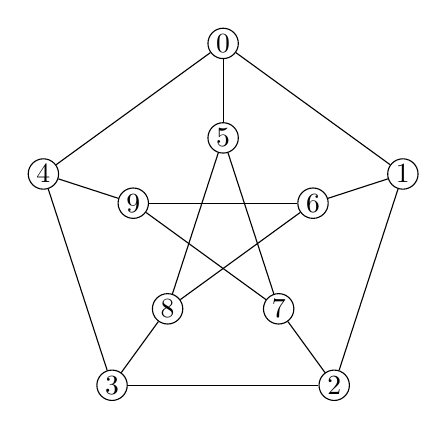
\begin{tikzpicture}[scale=1.2]

% Outer 5-cycle
\foreach \i/\name in {90/0, 18/1, 306/2, 234/3, 162/4}
  \node[draw, circle, inner sep=1pt] (\name) at ({2*cos(\i)}, {2*sin(\i)}) {\name};

% Inner 5-cycle
\foreach \i/\name in {90/5, 18/6, 306/7, 234/8, 162/9}
  \node[draw, circle, inner sep=1pt] (\name) at ({1*cos(\i)}, {1*sin(\i)}) {\name};

% Edges
\foreach \i/\j in {0/1, 1/2, 2/3, 3/4, 4/0} \draw (\i) -- (\j);
\foreach \i/\j in {5/7, 7/9, 9/6, 6/8, 8/5} \draw (\i) -- (\j);
\foreach \i/\j in {0/5, 1/6, 2/7, 3/8, 4/9} \draw (\i) -- (\j);

\end{tikzpicture}
\caption{Petersen graph}
\label{fig:petersen}
\end{minipage}
\hfill
\begin{minipage}{0.45\textwidth}
\centering
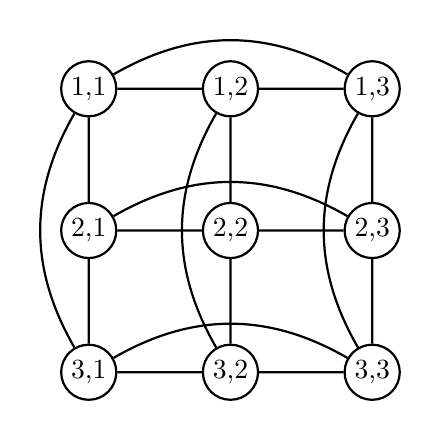
\begin{tikzpicture}[scale=1.2, every node/.style={circle, draw, inner sep=1pt, minimum size=0.7cm}, thick]

% Rook graph R(3)
\node (v11) at (-0.5, 3.5) {1,1}; \node (v12) at (1, 3.5) {1,2}; \node (v13) at (2.5, 3.5) {1,3};
\node (v21) at (-0.5, 2) {2,1}; \node (v22) at (1, 2) {2,2}; \node (v23) at (2.5, 2) {2,3};
\node (v31) at (-0.5, 0.5) {3,1}; \node (v32) at (1, 0.5) {3,2}; \node (v33) at (2.5, 0.5) {3,3};

\foreach \i in {1,2,3} {
  \foreach \j [count=\k from 2] in {1,2} {
    \draw (v\i\j) -- (v\i\k);
  }
}
\foreach \j in {1,2,3} {
  \foreach \i [count=\k from 2] in {1,2} {
    \draw (v\i\j) -- (v\k\j);
  }
}

\draw[bend right] (v11) to (v31);
\draw[bend left] (v11) to (v13);
\draw[bend right] (v13) to (v33);
\draw[bend left] (v31) to (v33);
\draw[bend right] (v12) to (v32);
\draw[bend left] (v21) to (v23);

\end{tikzpicture}
\caption{Rook graph $R(3)$}
\label{fig:rook-graph}
\end{minipage}

\vspace{1.2em}

% Second row: T(4) and T(4) \ {1,2}
\begin{minipage}{0.45\textwidth}
\centering
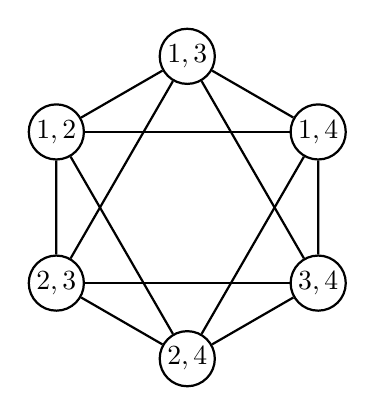
\begin{tikzpicture}[scale=1.2, every node/.style={circle, draw, inner sep=1pt, minimum size=0.7cm}, thick]

\foreach \i/\name in {90/13, 30/14, 330/34, 270/24, 210/23, 150/12}
  \node (l\name) at ({1.6*cos(\i)}, {1.6*sin(\i)}) 
  {$\pgfmathparse{int(\name/10)}\pgfmathresult,\pgfmathparse{int(mod(\name,10))}\pgfmathresult$};

\draw (l12) -- (l13);
\draw (l12) -- (l14);
\draw (l12) -- (l23);
\draw (l12) -- (l24);
\draw (l13) -- (l14);
\draw (l13) -- (l23);
\draw (l13) -- (l34);
\draw (l14) -- (l24);
\draw (l14) -- (l34);
\draw (l23) -- (l24);
\draw (l23) -- (l34);
\draw (l24) -- (l34);

\end{tikzpicture}
\caption{Triangular graph \(T(4)\)}
\label{fig:t4}
\end{minipage}
\hfill
\begin{minipage}{0.45\textwidth}
\centering
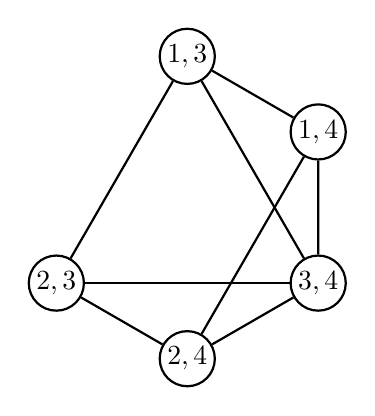
\begin{tikzpicture}[scale=1.2, every node/.style={circle, draw, inner sep=1pt, minimum size=0.7cm}, thick]

\foreach \i/\name in {90/13, 30/14, 330/34, 270/24, 210/23}
  \node (r\name) at ({1.6*cos(\i)}, {1.6*sin(\i)}) 
  {$\pgfmathparse{int(\name/10)}\pgfmathresult,\pgfmathparse{int(mod(\name,10))}\pgfmathresult$};

\draw (r13) -- (r14);
\draw (r13) -- (r23);
\draw (r13) -- (r34);
\draw (r14) -- (r24);
\draw (r14) -- (r34);
\draw (r23) -- (r24);
\draw (r23) -- (r34);
\draw (r24) -- (r34);

\end{tikzpicture}
\caption{$T(4)$ with vertex $\{1,2\}$ deleted}
\label{fig:t4'}
\end{minipage}

% \caption{Top: Petersen and Rook graphs. \quad Bottom: The triangular graph \(T(4)\) and its induced subgraph without vertex \(\{1,2\}\).}
\label{fig:grid-graphs}
\end{figure}












% \begin{figure}[h!]
% \centering
% \begin{tikzpicture}[scale=1.5, every node/.style={circle, draw, inner sep=1.5pt, minimum size=0.8cm}, every path/.style={thick}]

% % Define coordinates for vertices
% \node (v11) at (0, 3) {1,1};
% \node (v12) at (1, 3) {1,2};
% \node (v13) at (2, 3) {1,3};

% \node (v21) at (0, 2) {2,1};
% \node (v22) at (1, 2) {2,2};
% \node (v23) at (2, 2) {2,3};

% \node (v31) at (0, 1) {3,1};
% \node (v32) at (1, 1) {3,2};
% \node (v33) at (2, 1) {3,3};

% % Draw edges for rows
% \foreach \i in {1,2,3} {
%     \foreach \j [count=\k from 2] in {1,2} {
%         \draw (v\i\j) -- (v\i\k);
%     }
% }

% % Draw edges for columns
% \foreach \j in {1,2,3} {
%     \foreach \i [count=\k from 2] in {1,2} {
%         \draw (v\i\j) -- (v\k\j);
%     }
% }

% % Add curved edges to connect the corners
% \draw[bend right] (v11) to (v31); % Connect (1,1) to (3,1)
% \draw[bend left] (v11) to (v13); % Connect (1,1) to (1,3)
% \draw[bend right] (v13) to (v33); % Connect (1,3) to (3,3)
% \draw[bend left] (v31) to (v33); % Connect (3,1) to (3,3)

% \draw[bend right] (v12) to (v32);
% \draw[bend left] (v21) to (v23);

% \end{tikzpicture}
% \caption{The Rook Graph $R(3)$}
% \label{fig:rook-graph}
% \end{figure}

% \begin{figure}[h!]
% \centering

% % --- Petersen Graph ---
% \begin{minipage}{0.45\textwidth}
% \centering
% \begin{tikzpicture}[scale=1]

% % Outer 5-cycle
% \foreach \i/\name in {90/0, 18/1, 306/2, 234/3, 162/4}
%   \node[draw, circle, inner sep=1pt] (\name) at ({2*cos(\i)}, {2*sin(\i)}) {\name};

% % Inner 5-cycle (star points)
% \foreach \i/\name in {90/5, 18/6, 306/7, 234/8, 162/9}
%   \node[draw, circle, inner sep=1pt] (\name) at ({1*cos(\i)}, {1*sin(\i)}) {\name};

% % Outer pentagon edges
% \foreach \i/\j in {0/1, 1/2, 2/3, 3/4, 4/0}
%   \draw (\i) -- (\j);

% % Inner star edges
% \foreach \i/\j in {5/7, 7/9, 9/6, 6/8, 8/5}
%   \draw (\i) -- (\j);

% % Spokes
% \foreach \i/\j in {0/5, 1/6, 2/7, 3/8, 4/9}
%   \draw (\i) -- (\j);

% \end{tikzpicture}
% \caption{Petersen graph}
% \end{minipage}
% \hfill
% % --- Rook Graph ---
% \begin{minipage}{0.45\textwidth}
% \centering
% \begin{tikzpicture}[scale=1.5, every node/.style={circle, draw, inner sep=1.5pt, minimum size=0.8cm}, thick]

% % Nodes
% \node (v11) at (0, 3) {1,1};
% \node (v12) at (1, 3) {1,2};
% \node (v13) at (2, 3) {1,3};

% \node (v21) at (0, 2) {2,1};
% \node (v22) at (1, 2) {2,2};
% \node (v23) at (2, 2) {2,3};

% \node (v31) at (0, 1) {3,1};
% \node (v32) at (1, 1) {3,2};
% \node (v33) at (2, 1) {3,3};

% % Row edges
% \foreach \i in {1,2,3} {
%     \foreach \j [count=\k from 2] in {1,2} {
%         \draw (v\i\j) -- (v\i\k);
%     }
% }

% % Column edges
% \foreach \j in {1,2,3} {
%     \foreach \i [count=\k from 2] in {1,2} {
%         \draw (v\i\j) -- (v\k\j);
%     }
% }

% % Diagonals and curved edges
% \draw[bend right] (v11) to (v31);
% \draw[bend left] (v11) to (v13);
% \draw[bend right] (v13) to (v33);
% \draw[bend left] (v31) to (v33);
% \draw[bend right] (v12) to (v32);
% \draw[bend left] (v21) to (v23);

% \end{tikzpicture}
% \caption{Rook graph $R(3)$}
% \label{fig:rook-graph}
% \end{minipage}

% \label{fig:petersen-vs-rook}
% \end{figure}
% \begin{figure}[h!]
% \centering
% \begin{tikzpicture}[scale=1.2, every node/.style={circle, draw, inner sep=1pt, minimum size=0.7cm}, thick]

% % --- T(4) (on the left) ---
% \foreach \i/\name in {
%   90/13, 30/14, 330/34, 270/24, 210/23, 150/12}
%   \node (l\name) at ({-2.8 + 1.6*cos(\i)}, {1 + 1.6*sin(\i)}) 
%   {$\pgfmathparse{int(mod(\name,10))}\pgfmathresult,\pgfmathparse{int(\name/10)}\pgfmathresult$};

% % Edges of T(4)
% \draw (l12) -- (l13);
% \draw (l12) -- (l14);
% \draw (l12) -- (l23);
% \draw (l12) -- (l24);
% \draw (l13) -- (l14);
% \draw (l13) -- (l23);
% \draw (l13) -- (l34);
% \draw (l14) -- (l24);
% \draw (l14) -- (l34);
% \draw (l23) -- (l24);
% \draw (l23) -- (l34);
% \draw (l24) -- (l34);

% % --- T(4) \ {1,2} (on the right) ---
% \foreach \i/\name in {
%   90/13, 30/14, 330/34, 270/24, 210/23}
%   \node (r\name) at ({2.8 + 1.6*cos(\i)}, {1 + 1.6*sin(\i)}) 
%   {$\pgfmathparse{int(mod(\name,10))}\pgfmathresult,\pgfmathparse{int(\name/10)}\pgfmathresult$};

% % Edges of T(4) \ {1,2}
% \draw (r13) -- (r14);
% \draw (r13) -- (r23);
% \draw (r13) -- (r34);
% \draw (r14) -- (r24);
% \draw (r14) -- (r34);
% \draw (r23) -- (r24);
% \draw (r23) -- (r34);
% \draw (r24) -- (r34);

% \end{tikzpicture}
% \caption{Left: The triangular graph \( T(4) \). \quad Right: The induced subgraph \( T(4) \setminus \{1,2\} \).}
% \label{fig:t4-and-minus12}
% \end{figure}




% \begin{figure}[h!]
% % \centering
% \begin{tikzpicture}[scale=1.6, every node/.style={circle, draw, inner sep=1.5pt, minimum size=0.8cm}, thick]
% % --- K4 (triangle layout, left) ---
% \node (B) at (-3,0) {2};                   % bottom left
% \node (C) at (0,0) {3};                      % bottom right
% \node (D) at (-1.5,2.6) {4};                % top vertex
% \node (A) at (-1.5,1.05) {1};               % center vertex

% % Edges of K4
% \draw (A) -- (B);
% \draw (A) -- (C);
% \draw (A) -- (D);
% \draw (B) -- (C);
% \draw (B) -- (D);
% \draw (C) -- (D);

% % --- T(4) (on the right) ---
% % Place vertices evenly on a circle, shifted right by +4.5 units
% \foreach \i/\name in {
%   90/13, 30/14, 330/34, 270/24, 210/23, 150/12}
%   \node (\name) at ({4.5 + 2*cos(\i)}, {1 + 2*sin(\i)}) 
%   {$\pgfmathparse{int(mod(\name,10))}\pgfmathresult,\pgfmathparse{int(\name/10)}\pgfmathresult$};

% % Draw edges (pairs of 2-subsets that intersect)
% \draw (12) -- (13);
% \draw (12) -- (14);
% \draw (12) -- (23);
% \draw (12) -- (24);
% \draw (13) -- (14);
% \draw (13) -- (23);
% \draw (13) -- (34);
% \draw (14) -- (24);
% \draw (14) -- (34);
% \draw (23) -- (24);
% \draw (23) -- (34);
% \draw (24) -- (34);

% \end{tikzpicture}
% \caption{The complete graph \(K_4\) and its corresponding triangular graph \(T(4)\).}
% \label{fig:k4-and-t4}
% \end{figure}

% \begin{figure}[h]
% \centering
% \begin{tikzpicture}[scale=1]

% % Outer 5-cycle
% \foreach \i/\name in {90/0, 18/1, 306/2, 234/3, 162/4}
%   \node[draw, circle, inner sep=1pt] (\name) at ({2*cos(\i)}, {2*sin(\i)}) {\name};

% % Inner 5-cycle (star points)
% \foreach \i/\name in {90/5, 18/6, 306/7, 234/8, 162/9}
%   \node[draw, circle, inner sep=1pt] (\name) at ({1*cos(\i)}, {1*sin(\i)}) {\name};

% % Outer pentagon edges
% \foreach \i/\j in {0/1, 1/2, 2/3, 3/4, 4/0}
%   \draw (\i) -- (\j);

% % Inner star edges
% \foreach \i/\j in {5/7, 7/9, 9/6, 6/8, 8/5}
%   \draw (\i) -- (\j);

% % Spokes connecting outer and inner nodes
% \foreach \i/\j in {0/5, 1/6, 2/7, 3/8, 4/9}
%   \draw (\i) -- (\j);

% \end{tikzpicture}
% \caption{The Petersen graph.}
% \label{fig:petersen}
% \end{figure}






% --- Acknowledgements ---
\newpage
\section*{Acknowledgements}
I would like to express my sincere gratitude to my supervisor, Asst Prof Gary Greaves for his guidance, encouragement, and insightful discussions throughout the course of this project. His expertise in algebraic graph theory and coherent configurations provided a strong foundation upon which this work was built and motivated upon.

I would also like to extend my deepest gratitude to my family, friends, and everyone who provided me with unwavering support and encouragement throughout the course of this project. Pursuing a research topic in mathematics can often feel daunting and isolating, but I was constantly uplifted by the belief and motivation offered by those around me. Their words of encouragement reminded me of the joy and beauty in mathematical thinking, especially during challenging moments.

While my passion for mathematics is enduring, it is the people behind the scenes — my mom who supported me unconditionally, my brother who always gave me the breaks I needed by playing games together, my girlfriend who never failed to cheer me up when I got stuck on my progress weekly despite her hectic work schedule, and those who shared in both my doubts and breakthroughs — who gave me the resilience to see this work through. This project definitely would not have been possible without them.

% --- Table of Contents ---
\newpage
\tableofcontents
\newpage

% --- Main Body Sections ---
\pagenumbering{arabic}
\section{Introduction}

In this paper, we investigate the coherent closure of graphs derived by performing graph operations on strongly regular graphs. We first discuss the motivation and why we choose to investigate such properties.

\subsection{Historical Motivation}

In 1782, the mathematician Leonhard Euler posed a question: There are 6 army regiments, each with 6 officers of varying ranks. Is there a way to arrange the 36 officers in a 6-by-6 square such that no row nor column have any repeated army regiments or ranks? \cite{euler-36-officers-problem}. This question, now known as Euler's 36 Officer problem, was deemed impossible at the time, but inspired the study of what we now know as Mutually Orthogonal Latin Squares. By definition, a Latin Square is a $n$-by-$n$ array filled with $n$ different symbols such that no rows or columns have a duplicate symbol. A common example is the famous Sudoku games, though it has a stronger restriction that each block can have no repeating symbols as well. Relating it back to the 36 officer problem, we introduce the concept of Mutually Orthogonal Latin Squares, where there are a collection of Latin Squares of order $n$ that when superimposed, do not have any repetition of symbols in 2 cells. We explain with an example.

\[
\begin{aligned}
    &L^{(1)} = \begin{bmatrix}
        1 & 2 & 3 & 4\\
        2 & 1 & 4 & 3\\
        3 & 4 & 1 & 2\\
        4 & 3 & 2 & 1
    \end{bmatrix}\quad 
    &L^{(2)} = \begin{bmatrix}
        1 & 2 & 3 & 4\\
        4 & 3 & 2 & 1\\
        2 & 1 & 4 & 3\\
        3 & 4 & 1 & 2
    \end{bmatrix}\quad
    &L^{(3)} = \begin{bmatrix}
        1&2&3&4\\
        3&4&1&2\\
        4&3&2&1\\
        2&1&4&3
    \end{bmatrix}
\end{aligned}
\label{MOLS of order 4}
\]

Here we have a set of Mutually Orthogonal Latin Squares of order 4, or MOLS(4). We can indeed verify that all 3 matrices are Latin Squares as no row or column has a repeating element. We now show orthogonality for the first 2 matrices by this rule:
\begin{align*}
    L^{\{1,2\}} &= [(a_{ij}, b_{ij})]\\
    &= \begin{bmatrix}
        (1,1) & (2,2) & (3,3) & (4,4)\\
        (2,4) & (1,3) & (4,2) & (3,1)\\
        (3,2) & (4,1) & (1,4) & (2,3)\\
        (4,3) & (3,4) & (2,1) & (1,2)
    \end{bmatrix}
\end{align*}
where $L^{(1)}=[a_{ij}]$ and $L^{(2)} = [b_{ij}]$ are the first pair of orthogonal latin squares shown above. The same procedure can be repeated to show orthogonality between $L^{(1)},L^{(3)}$ and $L^{(2)},L^{(3)}$. 

\[
\begin{aligned}
    L^{\{1,3\}} =
    \begin{bmatrix}
        (1,1) & (2,2) & (3,3) & (4,4)\\
        (2,3) & (1,4) & (4,1) & (3,2)\\
        (3,4) & (4,3) & (1,2) & (2,1)\\
        (4,2) & (3,1) & (2,4) & (1,3)
    \end{bmatrix}\quad\quad
    L^{\{2,3\}} =
    \begin{bmatrix}
        (1,1) & (2,2) & (3,3) & (4,4)\\
        (4,3) & (3,4) & (2,1) & (1,2)\\
        (2,4) & (1,3) & (4,2) & (3,1)\\
        (3,2) & (4,1) & (1,4) & (2,3)
    \end{bmatrix}
\end{aligned}
\]As we can see, this is clearly the problem that Euler deemed impossible, just of an order of 6. 

\newpage
Interestingly, it has been proven that for any prime power $q=p^k$, there exist $q-1$ MOLS$(q)$. The construction uses the finite field $\mathbb{F}_q$, where each Latin square is defined using elements $a_i,a_j,a_k\in\mathbb{F}_q$. For the $k$-th Latin square $L^{(k)}$ of order $q$, the entry in row $i$ and column $j$ is given by
\begin{equation*}
    L^{(k)}_{i,j} = a_i+a_ka_j,\quad\text{for }i,j\in[q], \text{ }k\in[q-1].
\end{equation*}

For any Latin Square $L=[a_{ij}]$, we write it as an array of the following form:
\[
\begin{aligned}
    \begin{bmatrix}
        1&1&\dots&1&2&2&\dots&3&\dots&n&n&\dots&n\\
        1&2&\dots&n&1&2&\dots&1&\dots&1&2&\dots&n\\
        a_{11}&a_{12}&\dots&a_{1n}&a_{21}&a_{22}&\dots&a_{31}&\dots&a_{n1}&a_{n2}&\dots&a_{nn}
    \end{bmatrix} \in \mathbb{N}^{3\times n^2}
\end{aligned}
\]
where the first and second row correspond to the $(i,j)$-th position of the element $a_{ij}$, which is positioned on the third row. This is an example of a orthogonal array of size $(3,n)$. Orthogonal arrays can actually be generalised to sizes $(m,n)$, and we study the properties by using incidence structures.

\subsection{From Orthogonal Arrays to Graphs}
For any orthogonal array OA$(m,n)$, we can construct block graphs using the columns of OA$(m.n)$, where 2 columns are adjacent if the columns have overlapping entries in any row. Interestingly enough, this construction of the orthogonal array block graph results in a Strongly Regular Graph \cite{Asgarli_2022}. In this paper we focus on the base case OA$(2,n)$.

We first display OA$(2,n)$:
\[
\begin{aligned}
    \text{OA}(2,n)\begin{bmatrix}
        1&1&\dots&1&2&2&\dots&2&3&\dots&n&n&\dots&n\\
        1&2&\dots&n&1&2&\dots&n&1&\dots&1&2&\dots&n\\
    \end{bmatrix} \in \mathbb{N}^{2\times n^2}
\end{aligned}
\]
We can interpret this combinatorially as sets of ordered pairs $\{1,2,\dots,n\}\times\{1,2,\dots,n\}$, each appearing once in each column of OA$(2,n)$. Following the block graph construction of this graph, any 2 columns are adjacent if the top row of the 2 columns are the same or the bottom row of the 2 columns are the same. This block graph construction of OA$(2,n)$ is precisely the Rook's Graph $R(n)$, which is the graph of how a rook moves on a $n\times n$ chessboard. We can see that each column can represent the $(i,j)$-th position of the chessboard, each columns joined by where the rook can move next.

\subsection{Strongly Regular Graphs}
Along with Rook Graphs, we also consider the Triangular Graph $T(n)$, which is also a strongly regular graph as our family of graphs in this paper. A \textbf{strongly regular graph} with parameters $(v,k,\lambda,\mu)$ is a simple, undirected graph on $v$ vertices such that each vertex has exactly $k$ neighbors, every pair of adjacent vertices shares $\lambda$ common neighbors, and every pair of non-adjacent vertices shares $\mu$ common neighbors.~\cite{godsil2001algebraic}. Strongly regular graphs have many interesting structures and properties, one important property being its relation between its strongly regular parameters and its adjacency matrix $A$, namely $A^2 = kI + \lambda A + \mu(J-I-A)$. A famous example of a strongly regular graph is the Petersen Graph, $\operatorname{SRG(10,3,0,1)}$. A visual representation of the Petersen graph can be found in Figure~\ref{fig:petersen}. The regularity of strongly regular graphs leads to adjacency matrices that generate a commutative algebra of dimension three, which induces a coherent closure~\cite{bannai1984algebraic, greaves2024coherentrankgrapheigenvalues}. 

% \subsection{Primary Goal}
% In their paper, Greaves and Yip \cite{greaves2024coherentrankgrapheigenvalues} studied graphs with 3 eigenvalues and the change in coherent rank upon switching blocks of the respective graphs. There they discovered that switching graphs of 3 eigenvalues resulted in large coherent rank, with some ranks being unbounded. As such, we choose to investigate if it is possible to obtain a general coherent closure when switching strongly regular graphs, as strongly regular graphs are a subset of graphs with 3 eigenvalues. We choose the rook graph and triangular graph, well-known examples of strongly regular graphs, and destroy their symmetry to obtain a more general coherent configuration. In particular, we use Seidel switching and vertex deletion to investigate the coherent rank of graphs modified from strongly regular graphs.

\subsection{Primary Goal}

It is well known that any regular graph with exactly three eigenvalues has a minimum coherent algebra of dimension three, and hence coherent rank 3. However, the behavior of \emph{nonregular} graphs with three eigenvalues is not well understood in this context. In particular, there is no known bound on how large the coherent rank of such graphs can be. One recent construction showing unbounded coherent rank involves switching cliques in block graphs derived from orthogonal arrays~\cite{greaves2024coherentrankgrapheigenvalues}.

This motivates the broader study of how small perturbations to graphs with low coherent rank — especially those with high symmetry — affect their coherent closures. In this project, we focus specifically on the case of the rook graph $R(n)$, which is a strongly regular graph with three eigenvalues and coherent rank 3. The rook graph also arises as the block graph of the orthogonal array OA$(2,n)$, which is the simplest possible orthogonal array construction. 

We investigate whether applying graph operations, such as Seidel switching and vertex deletion, to $R(n)$ and to the triangular graph $T(n)$ can result in a general coherent configuration with significantly higher coherent rank. Our work explores whether these structured yet minimal modifications are sufficient to break the algebraic symmetry in a way that increases the complexity of the coherent closure. In doing so, we aim to contribute to the broader question: \emph{How does switching graphs, initially with low coherent rank, change its coherent rank?}

\newpage

\section{Notations and Definitions}

\subsection{Notations}

\begin{itemize}
    \item We denote the set comprising of integers from 1 to $n$ as $[n]$.
    \item We denote by \( I_n \), \( J_n \), \( O_n \), and \( \mathbf{1}_n \) the identity matrix, all-ones matrix, zero matrix, and all-ones (column) vector of order \( n \), respectively. We simply write \( I \), \( J \), \( O \), and \( \mathbf{1} \) when the order is clear from context, or in the case of \( J \) and \( O \), when the matrix is not square.

    \item We denote by \( e_{i,n} \) the elementary vector of size \( n \) with a \( 1 \) in the \( i \)-th position and \( 0 \) elsewhere.
    
    \item \(K_{n}\) denotes a Complete Graph of size $n$.
    
    \item \( A \otimes B \) denotes the Kronecker product of matrices \( A \) and \( B \). If \( A \in \mathbb{Q}^{m \times n} \) and \( B \in \mathbb{Q}^{p \times q} \), then:
    \[
    A \otimes B =
    \begin{bmatrix}
    a_{11}B & \cdots & a_{1n}B \\
    \vdots & \ddots & \vdots \\
    a_{m1}B & \cdots & a_{mn}B
    \end{bmatrix}
    \in \mathbb{Q}^{mp \times nq}.
    \]

    \item For any graph $\Gamma$, we denote the adjacency matrix of the graph as $A(\Gamma)$.

    \item Let $\langle A_1,\dots,A_n \rangle$ denote $\operatorname{span}\{A_1,\dots,A_n\}$, for some matrices $A_i$.

    \item We denote the Complete Graph on $n$ vertices as $K_n$.

    \item We will use the symbol $v_1\sim v_2$ to show adjacency between vertices $v_1$ and $v_2$.

    \item For any Strongly Regular Graph with parameters $(v,k,\lambda,\mu)$, we will denote them simply as $\operatorname{SRG}(v,k,\lambda,\mu)$. It denotes a graph $G=(V,E)$ such that $|V|=v$, each vertex has a degree of $k$, with adjacent vertices having $\lambda$ common neighbours, and non-adjacent vertices having $\mu$ common neighbours.
\end{itemize}


\subsection{Coherent Configuration and Algebras}
A \textit{coherent configuration} \cite{greaves2024coherentrankgrapheigenvalues} is a combinatorial and algebraic structure defined on a finite set \( V \). It provides a framework for studying symmetry and regularity in graphs and other relational structures. Formally, a coherent configuration is a pair \( (V, \mathcal{R}) \), where \( \mathcal{R} = \{R_1, \ldots, R_r\} \) is a partition of \( V \times V \) into binary relations, each represented by its adjacency matrix \( A_i \). These matrices satisfy the following axioms:

\subsubsection*{Axioms of a Coherent Configuration}

\begin{definition} \label{def:coherent-configuration}
Let $V$ be a finite set and $\mathcal{R}=\{R_1,\dots,R_r\}$ be a set of binary relations. For each $R_i$, let $W_i\in\operatorname{Mat}_V(\{0,1\})$ be defined such that its $(x,y)$-th entry is 1 if $(x,y)\in R_i$ and 0 otherwise. Suppose the following 4 conditions
\begin{itemize}
    \item[(CC1)] \quad \( \sum_{i=1}^{r} W_i = J \);
    \item[(CC2)] \quad For each \( i \in [r] \), there exists \( j \in [r] \) such that \( W_i^T = W_j \);
    \item[(CC3)] \quad There exists a subset \( \Delta \subseteq [r]\) such that \( \sum_{i \in \Delta} W_i = I \);
    \item[(CC4)] \quad \( W_i W_j = \sum_{k=1}^{r} p^k_{i,j} W_k \) for some constants \( p^k_{i,j} \in \mathbb{Z}_{\geq 0} \), for all \( i, j \in [r] \).
\end{itemize}
\end{definition}
Then $(V,\mathcal{R})$ is called a \textbf{coherent configuration} of \textbf{rank} $|\mathcal{R}|=r$. The set $V$ is called the \textbf{point-set} of the coherent configuration.

For each $i \in \Delta$, we call the subset $V_i := \{ x \in V : (x,x) \in R_i \}$ a \textbf{fibre} of the coherent configuration. It can be observed that the fibres form a partition of the point-set $V$. When $|\Delta| = 1$, the coherent configuration $(V, R)$ is called an \textbf{association scheme}. It follows from (CC4) that, for each $k \in [r]$, there exists $i$ and $j$ such that $R_k \subset V_i \times V_j$. Thus, each subset $\Delta' \subset \Delta$ induces a coherent configuration with point-set $\bigcup_{i \in \Delta'} V_i$. The \textbf{type} of $(V, \mathcal{R})$ is defined to be the matrix in $\mathrm{Mat}_\Delta(\mathbb{N})$ whose $(i,j)$-entry $t_{ij}$ is equal to the cardinality $|\{ k : R_k \subset V_i \times V_j \}|$. Note that the sum of the entries of the type matrix is equal to $r$. Furthermore, since the type matrix must be symmetric, we omit the entries below the diagonal. Higman~\cite{Higman19} established the following restriction on the type matrix.

\begin{lemma} \label{lemma:t_ii}
\textit{For each $i,j \in \Delta$, if $t_{ii} \leq 5$ and $t_{jj} \leq 5$ then $t_{ij} \leq \min(t_{ii}, t_{jj})$.}
\end{lemma}

\begin{definition}
    A \textbf{coherent algebra} is a matrix algebra $\mathcal{A} \subset \mathrm{Mat}_{V}(\mathbb{C})$ that satisfies the following axioms.

    \begin{itemize}
        \item $I, J \in \mathcal{A}$;
        \item $M^\top \in \mathcal{A}$ for each $M \in \mathcal{A}$;
        \item $MN \in \mathcal{A}$ and $M \circ N \in \mathcal{A}$ for each $M, N \in \mathcal{A}$, where $\circ$ denotes the entrywise product.
    \end{itemize}
\end{definition}

Each coherent algebra $\mathcal{A}$ has a unique basis of $\{0,1\}$-matrices $\{W_1, \ldots, W_r\}$ that corresponds to a coherent configuration $(V_\mathcal{A}, \mathcal{R}_\mathcal{A})$. We denote by $\mathcal{F}_\mathcal{A}$ the set of fibres of the coherent configuration $(V_\mathcal{A}, \mathcal{R}_\mathcal{A})$, and we define the \textbf{type} of $\mathcal{A}$ to be that of $(V_\mathcal{A}, \mathcal{R}_\mathcal{A})$. We note that the intersection of any two coherent algebras is itself a coherent algebra. Thus we define the \textbf{coherent closure} $\mathcal{W}(\Gamma)$ of $\Gamma$ to be the minimal coherent algebra that contains the adjacency matrix $A(\Gamma)$ of $\Gamma$. We write $\mathcal{W}(\Gamma) = \langle W_1, \ldots, W_r \rangle$, where $\{W_1, \ldots, W_r\}$ is the unique basis of $\{0,1\}$-matrices for $\mathcal{W}(\Gamma)$.

% Remember to cite
To show that a coherent algebra is minimal, we use the Wielandt's Principle \cite{wielandt} to derive a lower bound of the coherent rank.
\begin{theorem} Wielandt's Principle \label{def:wielandt-priniple} \\
    Let $\mathcal{A}$ be a coherent algebra and let $A\in\mathcal{A}$. For $b\in\mathbb{C}$, define the matrix $B$ such that:
    \begin{equation*}
        [B]_{xy}=\begin{cases}
            1,\quad\text{if }[A]_{xy}=b,\\
            0,\quad\text{otherwise}
        \end{cases}
    \end{equation*}
    then, $B\in\mathcal{A}$.
\end{theorem}

\subsection{Weisfeiler-Leman Algorithm}

The Weisfeiler-Leman (WL) refinement algorithm is a combinatorial method originally developed for graph isomorphism testing, which iteratively refines colorings on tuples of vertices based on their neighborhoods. For a given dimension \(k\), the \(k\)-WL algorithm operates on \(k\)-tuples in \(V^k\) and produces increasingly fine partitions of the tuple space as the algorithm stabilizes. In the context of coherent closure, the case \(k = 2\) is of particular interest. When applied to a graph \(\Gamma=(V,E)\), the 2-WL algorithm refines the coloring on \(V \times V\), beginning from an initial coloring that distinguishes edges, non-edges, and diagonal elements. At each iteration, the coloring of a pair \((x, y)\) is updated based on the multiset of colors of vertices \(z\) such that \((x, z)\) and \((z, y)\) are considered. This refinement continues until a stable partition is reached.

The key significance of the 2-WL algorithm lies in its equivalence to generating the \emph{coherent closure} of a graph. That is, the final coloring produced by 2-WL corresponds to a coherent configuration whose basis relations partition \(V \times V\) in a way that is closed under transpose and composition — the defining properties of a coherent configuration. This connection is formalized by the following result, adapted from Theorem 4.6.19 in \cite{ponomarenko_ccnotes}, where it implies that the 2-WL refinement captures the same structure as the 2-closure of a graph, and thus the coherent closure of \(\Gamma\) may be computed via the 2-dimensional WL algorithm.

To support our theoretical investigation, we leveraged computational tools to compute the coherent closure of graphs under various operations. Specifically, we utilised SageMath alongside the C++ implementation of the k-WL refinement algorithm available at \url{https://github.com/sven-reichard/stabilization/blob/master/weisfeiler.org} \cite{reichard_weisfeiler}. This allowed us to efficiently compute the 2-WL stabilization of graphs and directly obtain their coherent closures for small values of $n$. Through these computations, we observed consistent patterns in the resulting coherent ranks across different graph modifications, which in turn guided the formal proofs presented in the following sections.


\subsection{Rook Graph}

\paragraph{General Rook Graph}
The \textbf{rook graph} \( R(m,n) = (V, E) \), where \( m \leq n \), is defined as the simple undirected graph formed possible moves of a rook on each cell of an \( m \times n \) chessboard. Formally, let 
\begin{equation*}
    V = \left\{\begin{pmatrix}
        i \\ j
    \end{pmatrix} :\quad i\in [m],j\in [n]\right\};
\end{equation*}
be the vertex set representing all cells on the $m\times n$ chessboard. The edge set is given by
\begin{equation*}
    E = \left\{
        \left\{
        \begin{pmatrix}i\\j\end{pmatrix}, \begin{pmatrix}k\\l\end{pmatrix}
        \right\}
        :\quad i=k \text{ or } j=l
    \right\}.
\end{equation*}
Then $R(m,n)$ is the rook graph.
\newpage

We can think of $R(n)$ as the following:
\begin{itemize}
    \item Each vertex corresponds to a cell on the chessboard, so the total number of vertices is \( |V| = mn \).
    \item Two vertices are adjacent if and only if they lie in the same row or the same column of the chessboard. 
\end{itemize}

The adjacency matrix of \( R(m,n) \) can be written in block form as:
\[
A(R(m,n)) = 
\underbrace{
\left[
\begin{array}{cccc}
J_{n} - I & I_n & \cdots & I_n \\
I_n & J_n - I & \cdots & I_n \\
\vdots & \vdots & \ddots & \vdots \\
I_n & I_n & \cdots & J_n - I
\end{array}
\right]
}_{\text{\( m \) blocks}}.
\]

\paragraph{Square Rook Graph}
A \textbf{square rook graph} is the special case where \( m = n \). We denote this as \( R(n) \).
An illustration of \( R(3) \) is provided in Figure~\ref{fig:rook-graph}.

\paragraph{Properties of the square rook graph}
\begin{itemize}
    \item \( R(n) \) is a strongly regular graph with parameters:
    \[
    \operatorname{SRG}(n^2, 2(n - 1), n - 2, 2)\quad \text{for }n \ge 3;
    \]
    \item Let $A$ be the adjacency matrix $R(n)$. Since it is strongly regular, $A^2 = 2(n-1)I + (n-2)A + 2(J-I-A)$.
\end{itemize}




% not sure if needed
% \paragraph{Construction of \(R(n)\)}

% Alternatively, \(R_{n,n}\) can be constructed using an orthogonal array of size \( \text{OA}(2, n) \), which has the following properties:
% \begin{itemize}
%     \item \( \text{OA}(2, n) \) is a \( 2 \times n^2 \) matrix, where each column corresponds to a unique pair \( (x, y) \in \{1, \dots, n\} \times \{1, \dots, n\} \).
%     \item For any two rows, every pair of entries appears exactly once in the same column.
% \end{itemize}

% We can visualise it as such:
% $$
% \text{OA}(2, n) = \begin{bmatrix}
%     1 & 1 & \cdots & 1 & 2 & 2 & \cdots & 2 & \cdots & n & n & \cdots & n \\
%     1 & 2 & \cdots & n & 1 & 2 & \cdots & n & \cdots & 1 & 2 & \cdots & n \\
% \end{bmatrix}
% $$

% \paragraph{}
% Given \( \text{OA}(2, n) \), we define the \textbf{Orthogonal Array graph} as follows:

% \begin{definition}
%     The Orthogonal Array graph, \(G_{OA} = (V,E)\), is constructed by OA\((2,n)\) by the following:
%     \begin{itemize}
%         \item Each vertex \( v_i \) corresponds to the \( i \)-th column of the orthogonal array, so \( |V| = n^2 \).
%         \item Two vertices \( v_i \) and \( v_j \) are adjacent if they share the same value in any row of the array.
%     \end{itemize}
% \end{definition}

% \paragraph{}
% For \( n = 3 \), the orthogonal array \( \text{OA}(2, 3) \) is:
% \[
% \begin{bmatrix}
% 1 & 1 & 1 & 2 & 2 & 2 & 3 & 3 & 3 \\
% 1 & 2 & 3 & 1 & 2 & 3 & 1 & 2 & 3
% \end{bmatrix}.
% \]


% The Orthogonal Array graph of OA\((2, 3)\) would have $9$ vertices in total, with each vertex being adjacent to 4 other vertices.
% (i.e. $\begin{pmatrix}
%     1\\1
% \end{pmatrix}$ is adjacent to $\begin{pmatrix}
%     1\\2
% \end{pmatrix}$, $\begin{pmatrix}
%     1\\3
% \end{pmatrix}$, $\begin{pmatrix}
%     2\\1
% \end{pmatrix}$ and $\begin{pmatrix}
%     3\\1
% \end{pmatrix}$)

% It can be observed that this construction of \(G\) is isomorphic to Rook graph \(R(3)\), and we can generalise it to \(R(n)\) as well.


% \begin{theorem}
%     A block graph construction of OA\((2,n)\) is isomorphic to \(R(n)\).
% \end{theorem}

% \begin{proof} 
% We want to show that the block graph construction of OA\((2,n)\), \(G = (V_G,E_G)\), is isomorphic to the Rook graph, \(R(n) = (V_R, E_R)\). \\ \\
% Given 
% \(
% \text{OA}(2, n) = \begin{bmatrix}
%     1 & 1 & \cdots & 1 & 2 & 2 & \cdots & 2 & \cdots & n & n & \cdots & n \\
%     1 & 2 & \cdots & n & 1 & 2 & \cdots & n & \cdots & 1 & 2 & \cdots & n \\
% \end{bmatrix},
% \) \\
% let $G = (V_G,E_G)$ be the block graph constructed using the steps defined above. \\

% We proceed as follows:
% \begin{enumerate}
%     \item \textbf{Vertex Sets}: 
%     Since the columns of OA\((2,n)\) spans \(\{1,2,\cdots,n\}^2\), \(|V| = n^2\). Similarly, the vertices of \(R_{n,n}\) correspond to the cells of an \(n \times n\) chessboard, so \(|V_R| = n^2\). Therefore, \(|V_G| = |V_R|\).

%     \item \textbf{Edge Sets}: 
%     In \(G\), two vertices are adjacent if their corresponding columns in OA\((2,n)\) share the same value in at least one row. This means that:
%     \begin{itemize}
%         \item If two vertices share the same value in the top row, they are adjacent.
%         \item If two vertices share the same value in the bottom row, they are adjacent.
%     \end{itemize}
%     This adjacency condition matches exactly how edges are defined in \(R(n)\), where two cells of the chessboard are connected if they lie in the same row or column. Thus, the adjacency relationships in \(G\) and \(R(n)\) are equivalent.

%     \item \textbf{Bijection}: 
    
%     \begin{itemize}
%         \item Let \((i,j) \in V_G\) represent an arbitrary column in OA\((2,n)\).
%         \item Let \((r_i,c_j) \in V_R\) represent a arbitrary position on a \(n\times n\) chessboard which corresponds to the \(i\)-th row and \(j\)-th column.
%     \end{itemize}
%     We now define a mapping \(f: V_G \to V_R\) as follows:
%     \begin{align*}
%         f((i,j)) &= (r_i,c_j), \text{  where \( (i,j) \in V_G \) and \((r_i,c_j) \in V_R\). }
%     \end{align*}
    
%     To show that the mapping is bijective, we show the following:
%     \begin{itemize}
%         \item \textbf{Injectivitiy}: \\
%         Assume \(f((i,j)) = f((i',j'))\). Then:
%         \[
%         f((i,j)) = (r_i, c_j) \quad \text{and} \quad f((i',j')) = (r_{i'}, c_{j'}).
%         \]
%         Since \(f((i,j)) = f((i',j'))\), it follows that:
%         \[
%         (r_i, c_j) = (r_{i'}, c_{j'}).
%         \]
%         Thus, \(r_i = r_{i'}\) and \(c_j = c_{j'}\), which implies \((i,j) = (i',j')\). 
%         In other words, if two positions on the \(n\times n\) chessboard are the same, their corresponding columns in the OA\((2,n)\) must be the same. \\
%         Therefore, \(f\) is injective.
    
%         \item \textbf{Surjectivity}: \\
%         Taking an arbitrary \((r_i,c_j) \in V_R\), we need to show that there exists a \((i,j) \in V_G\) such that \(f((i,j)) = (r_i,c_j)\). \\
%         Note that \((r_i,c_j)\) corresponds to the position on the chessboard with row \(i\) and column \(j\). Since \(f\) maps a column to a chessboard position uniquely, the 
%         Since we have shown injectivity, for each \((i,j) \in V_G\), there is a one-to-one \(f((i,j)) = (r_i,c_j) \in V_R\). Thus, the set of images \(\{f((i,j))\text{ } | \text{ }(i,j) \in V_G\} \subseteq V_R\) contains exactly \(n^2\) elements. We have also shown
%         Let \((x, y) \in V_R\) be an arbitrary vertex in \(R(n)\). By the construction of OA\((2, n)\), there exists a column \(c = \begin{bmatrix} x \\ y \end{bmatrix} \in V\) such that the top row contains \(x\) and the bottom row contains \(y\). Thus, \(f(c) = (x, y)\), meaning every vertex in \(V_R\) has a preimage in \(V_G\). \\
%         Therefore, \(f\) is surjective.
%     \end{itemize} 
%     Thus, we have shown that the mapping $f$ is a bijection.

%     \item \textbf{Adjacency Preservation}: 
%     If two vertices in \(G\) are adjacent, they share the same value in the top or bottom row of OA\((2,n)\). Under the mapping \(f\), this means the corresponding vertices in \(R(n)\) share the same row or column. Similarly, if two vertices in \(R(n)\) are adjacent, their positions share the same row or column, which corresponds to adjacency in \(G\). Thus, \(f\) preserves adjacency.

% \end{enumerate}
% Therefore, since $f$ is a bijection from $V_G\to V_R$ such that the edges are preserved, $G\cong R_{n,n}$.
    
% \end{proof}
\subsection{Triangular Graph}

The \textbf{triangular graph} \( T(n) \) is defined as the graph whose vertices correspond to the $2$-element subsets of an $n$-element set. Two vertices are adjacent if and only if the corresponding subsets intersect in exactly one element.

Formally, let
\[
V = \left\{ \{i,j\} :\quad 1 \le i < j \le n \right\}
\]
be the vertex set of all unordered pairs from the set $[n] = \{1, 2, \dots, n\}$. The edge set is given by
\[
E = \left\{ \left\{ \{i,j\}, \{k,\ell\} \right\} :\quad |\{i,j\} \cap \{k,\ell\}| = 1 \right\}.
\]
Then \( T(n) = (V, E) \) is the triangular graph. An illustration of $T(4)$ and its resulting graph when we delete the vertex $\{1,2\}$ can be seen in Figures~\ref{fig:t4} and \ref{fig:t4'}.

\paragraph{Properties}
\begin{itemize}
    \item \( T(n) \) is a \emph{strongly regular graph} with parameters
    \[
    \operatorname{SRG} \left( \frac{n(n-1)}{2}, 2(n-2), n-2, 4 \right), \quad \text{for } n \ge 4.
    \]
\end{itemize}

\newpage

\section{Vertex Deletion and Coherent Configurations}
In this section, we perform vertex deletion on $R(n)$ and $T(n)$ and investigate its coherent closure.
\subsection{Deleting 1 Vertex in \texorpdfstring{$R(n)$}{R(n)}}
Here, we apply vertex deletion on $R(n)$ witth respect to 1 vertex. We then investigate its resulting adjacency matrix structure and make a claim about its coherent closure.
\subsubsection{Graph Construction}

Rook graphs are vertex-transitive \cite{godsil2001algebraic}, so we choose any vertex to be deleted. For simplicity, let \( v_1 \), corresponding to the cell \( \begin{pmatrix} 1 \\ 1 \end{pmatrix} \), be deleted. This resulting graph will be denoted as $\Gamma_1$.

We choose to partition the remaining vertices according to their adjacency with the chosen $v_1$:
\begin{enumerate}
    \item The \( 2(n-1) \) vertices adjacent to \( v_1 \), corresponding to the set:
    \begin{align*}
        \left\{ \begin{pmatrix} 1 \\ 2 \end{pmatrix}, \begin{pmatrix} 1 \\ 3 \end{pmatrix},..., \begin{pmatrix} 1 \\ n \end{pmatrix}, \begin{pmatrix} 2 \\ 1 \end{pmatrix}, \begin{pmatrix} 3 \\ 1 \end{pmatrix},..., \begin{pmatrix} n \\ 1 \end{pmatrix} \right\}.
    \end{align*} \\
    We shall call this set $V_1$.
    \item The remaining \( (n-1)^2 \) vertices, corresponding to the set:
    \begin{align*}
        \left\{ \begin{pmatrix} 2 \\ 2 \end{pmatrix}, \begin{pmatrix} 2 \\ 3 \end{pmatrix},...,\begin{pmatrix} 2 \\ n \end{pmatrix},\begin{pmatrix} 3 \\ 2 \end{pmatrix}, \begin{pmatrix} 3 \\ 3 \end{pmatrix},...,\begin{pmatrix} 3 \\ n \end{pmatrix},...,\begin{pmatrix} n \\ 2 \end{pmatrix}, \begin{pmatrix} n \\ 3 \end{pmatrix},...,\begin{pmatrix} n \\ n \end{pmatrix} \right \}.
    \end{align*} \\
    We shall call this set $V_2$.
\end{enumerate}

% \subsection{Adjacency Matrix Partitioning}
By grouping the vertices corresponding to $V_1$ and $V_2$ together, we end up with a matrix decomposition:
\[
A(\Gamma_1) =
\begin{bmatrix}
A_1 & C \\
C^T & A_2
\end{bmatrix},
\]
We will now aim to obtain the adjacency matrix $A(\Gamma_1)$ by determining the structure of matrices $A_1, A_2$ and $C$.

\begin{proposition}
    $A_1$ is the adjacency matrix of two disjoint \(K_{n-1}\).
    \end{proposition}
\begin{proof}
    The set $V_1$ contains vertices: \\
    \begin{align*}
        V_1 = \left\{ \begin{pmatrix} 1 \\ 2 \end{pmatrix}, \begin{pmatrix} 1 \\ 3 \end{pmatrix},..., \begin{pmatrix} 1 \\ n \end{pmatrix}, \begin{pmatrix} 2 \\ 1 \end{pmatrix}, \begin{pmatrix} 3 \\ 1 \end{pmatrix},..., \begin{pmatrix} n \\ 1 \end{pmatrix} \right\}
    \end{align*}
    Let us split the set into disjoint subsets \(L\) and \(R\):
    \begin{align*}
        L &= \left\{ \begin{pmatrix} 1 \\ 2 \end{pmatrix}, \begin{pmatrix} 1 \\ 3 \end{pmatrix},..., \begin{pmatrix} 1 \\ n \end{pmatrix}\right\} = \left \{ \begin{pmatrix} 1 \\ i \end{pmatrix} : \text{ }i \in [n]\setminus\{1\}\right \}, \\ \\
        R &= \left\{ \begin{pmatrix} 2 \\ 1 \end{pmatrix}, \begin{pmatrix} 3 \\ 1 \end{pmatrix},..., \begin{pmatrix} n \\ 1 \end{pmatrix} \right\} = \left \{ \begin{pmatrix} j \\ 1 \end{pmatrix} : \text{ }j \in [n]\setminus\{1\}\right \}
    \end{align*}
    \begin{itemize}
        \item \textbf{Show disjointness of graphs}: \\
        Let \(v_L = \begin{pmatrix} 1 \\ i \end{pmatrix}\in L\) and \(v_R = \begin{pmatrix} j \\ 1 \end{pmatrix} \in R\), such that \(i, j \in [n]\setminus\{1\}\). For any \(v_L\) and \(v_R\), \(i \neq 1\) and \(j \neq 1\), and thus \(v_L\) will not be adjacent to \(v_R\), showing that there are no edges between the vertex sets \(L \text{ and } R\) $\Longrightarrow$ Graphs induced by vertices in $L$ and $R$ are disjoint.
        
        \item \textbf{Show that the disjoint graphs are both \(K_{n-1}\)}:
        \begin{itemize}
            \item For the vertex set $L$\\
            Notice that the vertices in \(L\) are adjacent to each other as the top row are all equal to 1, \(v_L = \begin{pmatrix} 1 \\ i \end{pmatrix}\in L\). Since \(|L| = n-1\), we conclude that the $n-1$ vertices in $L$ are adjacent to each other, which is the definition of $K_{n-1}$.
            \item For the vertex set $R$\\
            Similar to the case of \(L\), we note that the vertices in \(R\) are adjacent to each other as the bottom row are all equal to 1, \(v_R = \begin{pmatrix} j \\ 1 \end{pmatrix} \in R\). Since \(|R| = n-1\), we conclude that the $n-1$ vertices in $R$ are adjacent to each other, which is the definition of $K_{n-1}$.
        \end{itemize}
    \end{itemize}
     We have shown that the graphs formed by vertex sets \(L\) and \(R\) are disjoint, and that each graph formed is \(K_{n-1}\). Thus we have:
     \begin{equation*}
         A_1 = 
         \begin{bmatrix}
             J_{n-1}-I & O_{n-1} \\
             O_{n-1} & J_{n-1}-I
         \end{bmatrix}
     \end{equation*}
\end{proof}

\begin{proposition}
    $A_2$ is the adjacency matrix of the square rook graph \(R(n-1)\).
\end{proposition}
\begin{proof} The set \(V_2\) contains vertices:
\begin{align*}
    V_2 = \left\{ \begin{pmatrix} 2 \\ 2 \end{pmatrix}, \begin{pmatrix} 2 \\ 3 \end{pmatrix},...,\begin{pmatrix} 2 \\ n \end{pmatrix},\begin{pmatrix} 3 \\ 2 \end{pmatrix}, \begin{pmatrix} 3 \\ 3 \end{pmatrix},...,\begin{pmatrix} 3 \\ n \end{pmatrix},...,\begin{pmatrix} n \\ 2 \end{pmatrix}, \begin{pmatrix} n \\ 3 \end{pmatrix},...,\begin{pmatrix} n \\ n \end{pmatrix} \right \}
\end{align*}
We can generalise this set into:
\begin{align*}
    V_2 &= \left \{ \begin{pmatrix} i \\ j \end{pmatrix}:\quad i \in [n]\setminus\{1\}, \quad j \in [n]\setminus\{1\}\right \} \\
    & = \left \{ \begin{pmatrix} i \\ j \end{pmatrix} :\quad i-1 \in [n-1],\quad j-1 \in [n-1]\right \} \\
\end{align*} \\
We will show that it is isomorphic to $R(n-1) = (V,E)$ by forming a bijection between $V_2$ and $V$. First we state the definition of $V$:
\begin{equation*}
    V = \left \{ \begin{pmatrix} i' \\ j' \end{pmatrix} : \text{ } i' \in [n-1], j' \in [n-1]\right \}
\end{equation*}
The bijection used here is 
\begin{equation*}
    f:V_2 \xrightarrow{} V, f\left(\begin{pmatrix} i \\ j \end{pmatrix}\right) = \begin{pmatrix} i-1 \\ j-1 \end{pmatrix}
\end{equation*}
In words, each cell $\begin{pmatrix} i \\ j \end{pmatrix}\in V_2$ is mapped to the cell $\begin{pmatrix} i' \\ j' \end{pmatrix}\in V$ where $\begin{pmatrix} i' \\ j' \end{pmatrix} = \begin{pmatrix} i-1 \\ j-1 \end{pmatrix}$.
\begin{itemize}
    \item Show $f$ is injective \\
    Let $\begin{pmatrix} i'_1 \\ j'_1 \end{pmatrix}, \begin{pmatrix} i'_2 \\ j'_2 \end{pmatrix}\in V$. We want to show if $\begin{pmatrix} i'_1 \\ j'_1 \end{pmatrix} = \begin{pmatrix} i'_2 \\ j'_2\end{pmatrix}$, then $\begin{pmatrix} i_1 \\ j_1 \end{pmatrix} = \begin{pmatrix} i_2 \\ j_2 \end{pmatrix}$:
    \begin{align*}
        \begin{pmatrix} i'_1 \\ j'_1 \end{pmatrix} = \begin{pmatrix} i'_2 \\ j'_2\end{pmatrix} \longrightarrow
        \begin{pmatrix} i_1-1 \\ j_1-1 \end{pmatrix} = \begin{pmatrix} i_2-1 \\ j_2 -1\end{pmatrix} \longrightarrow
        \begin{pmatrix} i_1 \\ j_1 \end{pmatrix} = \begin{pmatrix} i_2 \\ j_2 \end{pmatrix} 
    \end{align*}
    Thus, $f$ is injective.

    \item Show $f$ surjective \\
    We want to show
    \begin{align*}
        \forall \begin{pmatrix}
            i'\\j'
        \end{pmatrix} \in V, \quad\exists \begin{pmatrix}
            i\\j
        \end{pmatrix} \in V_2 \quad\text{such that}\quad f\left(\begin{pmatrix} i \\ j \end{pmatrix}\right) = \begin{pmatrix}
            i'\\j'
        \end{pmatrix}
    \end{align*}
    We have shown that \( f \) is injective. Since the domain \( V_2 \) and codomain \( V \) both have cardinality \( (n-1)^2 \), it follows that the image \( f(V_2) \subseteq V \) must also have size \( (n-1)^2 \).

    Thus, \( f(V_2) = V \), and \( f \) is surjective.

    \item Show Adjacency preservation\\
    Let $E_2$ be the edge set of the graph with adjacency matrix $A_2$. Let $\left\{\begin{pmatrix}i_1\\j_1\end{pmatrix},  \begin{pmatrix}i_2\\j_2\end{pmatrix}\right\}\in E_2$. This implies $i_1=i_2$ or $j_1=j_2$. Under $f$, 
    \begin{align*}
        \left\{f\left(\begin{pmatrix}i_1\\j_1\end{pmatrix}\right),  f\left(\begin{pmatrix}i_2\\j_2\end{pmatrix}\right)\right\}
        &= \left\{\begin{pmatrix}i_1-1\\j_1-1\end{pmatrix},  \begin{pmatrix}i_2-1\\j_2-1\end{pmatrix}\right\}
    \end{align*}
    Since $i_1=i_2$ or $j_1=j_2$, $i_1-1=i_2-1$ or $j_1-1=j_2-1$ and so
    \begin{equation*}
        \left\{\begin{pmatrix}i_1-1\\j_1-1\end{pmatrix},  \begin{pmatrix}i_2-1\\j_2-1\end{pmatrix}\right\} \in E
    \end{equation*}
    Thus adjacency is preserved under $f$ as well.
\end{itemize}
Since $V_2$ has a bijective mapping to $V$ and adjacency is preserved under said mapping, we have shown that the graph with adjacency matrix $A_2$ is isomorphic to $R(n-1)$. So we conclude that:
\begin{equation*}
    A_2 = 
        \underbrace{
        \left[
        \begin{array}{cccc}
        J_{n-1} - I & I_{n-1} & \cdots & I_{n-1} \\
        I_{n-1} & J_{n-1} - I & \cdots & I_{n-1} \\
        \vdots & \vdots & \ddots & \vdots \\
        I_{n-1} & I_{n-1} & \cdots & J_{n-1} - I
        \end{array}
        \right]
        }_{\text{\( n-1 \) blocks}}
\end{equation*}
\end{proof}

We now aim to construct the matrix $C$.
\paragraph{Construction of \texorpdfstring{$C$}{C}}
We know the rows of \(C\) are indexed by the set \(V_1\) and columns are indexed by the set \(V_2\). To make things simple, we consider this decomposition of $C$:

\begin{equation*}
    C = \begin{bmatrix}
        C_1\\C_2
    \end{bmatrix}
\end{equation*}

where the top half of \(C\) is denoted by \(C_1\) with rows indexed by the set \(L\) and columns indexed by \(V_2\), while the bottom half is denoted by \(C_2\) with rows indexed by the set \(R\) and columns indexed by \(V_2\)

\paragraph{\texorpdfstring{$C_1$}{C1}}

For \( C_1 \), the rows are indexed by:
\begin{align*}
    L &= \left\{\begin{pmatrix} 1 \\ 2 \end{pmatrix}, \begin{pmatrix} 1 \\ 3 \end{pmatrix}, \dots, \begin{pmatrix} 1 \\ n \end{pmatrix}\right\} \\
    &= \left\{ \begin{pmatrix}1 \\ i\end{pmatrix}:\quad i\in[n]\setminus\{1\}\right\},
\end{align*}

while the columns are indexed by:
\begin{align*}
    V_2 &= \left\{\begin{pmatrix} 2 \\ 2 \end{pmatrix}, \begin{pmatrix} 2 \\ 3 \end{pmatrix}, \dots, \begin{pmatrix} 2 \\ n \end{pmatrix}, \begin{pmatrix} 3 \\ 2 \end{pmatrix}, \dots, \begin{pmatrix} n \\ n \end{pmatrix}\right\} \\
    &= \left\{\begin{pmatrix}j \\k\end{pmatrix}:\quad j,k\in[n]\setminus\{1\}\right\}.
\end{align*}

\begin{proposition}
    Each vertex corresponding to an element in \(L\) has exactly \( n-1 \) adjacent vertices corresponding to \(n-1\) elements in \(V_2\).
\end{proposition}
\begin{proof}
    We aim to show any \(v_L = \begin{pmatrix}1\\i\end{pmatrix} \in L\) is adjacent to exactly \(n-1\) \(v_2 = \begin{pmatrix}j\\k\end{pmatrix} \in V_2\). \\
    Given \(v_L = \begin{pmatrix}1\\i\end{pmatrix}\) and \(v_2 = \begin{pmatrix}j\\k\end{pmatrix}\), when \(i = k\), \(v_L\) is adjacent to \(v_2\). This is the only case where adjacency occurs as \(j\neq 1, j\in[n]\setminus\{1\}\). \\
    Furthermore, there are \(n-1\) edges for any \(v_L\). When we set \(i=k\), there are \(|[n]\setminus\{1\}|=n-1\) possible values of \(j\). \\
    Thus, for any \(v_L\) there are exactly \(n-1\) adjacent vertices \(v_2\).
\end{proof}
For instance, when we fix \(i=k=2\):
\[
\begin{pmatrix} 1 \\ 2 \end{pmatrix} \text{ is adjacent to } \begin{pmatrix} 2 \\ 2 \end{pmatrix}, \begin{pmatrix} 3 \\ 2 \end{pmatrix}, \dots, \begin{pmatrix} n \\ 2 \end{pmatrix}.
\]

This adjacency results in rows of the form:
\[
[e_{1,n-1}^T \quad e_{2,n-1}^T \quad e_{3,n-1}^T \quad \cdots \quad e_{n-1,n-1}^T]. 
\]

When repeated for \( \begin{pmatrix} 1 \\ 3 \end{pmatrix} \) onwards, \( C_1 \) is composed of \( n-1 \) blocks of \( I^{(n-1)} \):
\[
C_1 = 
\begin{bmatrix}
I_{n-1} & I_{n-1} & \cdots & I_{n-1}
\end{bmatrix}.
\]

Explicitly, \( \mathbf{C_1} \) looks like:
\[
C_1 = 
\begin{bmatrix}
1 & 0 & \cdots & 0 & 1 & 0 & \cdots & 0 & \cdots & 1 & 0 & \cdots & 0 \\
0 & 1 & \cdots & 0 & 0 & 1 & \cdots & 0 & \cdots & 0 & 1 & \cdots & 0 \\
\vdots & \vdots & \ddots & \vdots & \vdots & \vdots & \ddots & \vdots & \cdots & \vdots & \vdots & \ddots & \vdots \\
0 & 0 & \cdots & 1 & 0 & 0 & \cdots & 1 & \cdots & 0 & 0 & \cdots & 1
\end{bmatrix}.
\]

\paragraph{\texorpdfstring{$C_2$}{C2}}

For \( C_2 \), the rows are indexed by:
\begin{align*}
R &= \left\{\begin{pmatrix} 2 \\ 1 \end{pmatrix}, \begin{pmatrix} 3 \\ 1 \end{pmatrix}, \dots, \begin{pmatrix} n \\ 1 \end{pmatrix}\right\} \\
&= \left\{\begin{pmatrix}i \\ 1\end{pmatrix}:\quad i\in[n]\setminus\{1\}\right\},
\end{align*}
while the columns are still indexed by \(V_2\). Following the same logic as in \(C_1\), we simply switch the logic from the bottom row to the top row to show adjacency.\\

This results in each row is adjacent to \( n-1 \) vertices, with \( 1 \)'s being contiguous. For instance:
\[
\begin{pmatrix} 2 \\ 1 \end{pmatrix} \text{ is adjacent to } \begin{pmatrix} 2 \\ 2 \end{pmatrix}, \begin{pmatrix} 2 \\ 3 \end{pmatrix}, \dots, \begin{pmatrix} 2 \\ n \end{pmatrix}.
\]
This results in rows of the form:
\[
[\underbrace{1 \quad 1 \quad \cdots \quad 1}_{n-1 \text{ elements}} \quad 0 \quad 0 \quad \cdots].
\]

Explicitly, \( C_2 \) looks like:
\[
C_2 = 
\begin{bmatrix}
1 & 1 & \cdots & 1 & 0 & 0 & \cdots & 0 & \cdots & 0 & 0 & \cdots & 0 \\
0 & 0 & \cdots & 0 & 1 & 1 & \cdots & 1 & \cdots & 0 & 0 & \cdots & 0 \\
\vdots & \vdots & \ddots & \vdots & \vdots & \vdots & \ddots & \vdots & \cdots & \vdots & \vdots & \ddots & \vdots \\
0 & 0 & \cdots & 0 & 0 & 0 & \cdots & 0 & \cdots & 1 & 1 & \cdots & 1
\end{bmatrix}.
\]

We can also condense this matrix $C_2$ into block form, denoted by $M_i\in\mathbb{R}^{(n-1)\times(n-1)}$, where the $i$-th row consists of 1s and 0s elsewhere.

\[
C_2 = 
\begin{bmatrix}
    M_1 & M_2 & M_3 &\dots& M_{n-1}
\end{bmatrix}
\]

Since $M_i\in\mathbb{R}^{(n-1)\times(n-1)}$, we can represent it as:
\begin{align*}
    M_i = 
    \begin{bmatrix}
    0&0&0&0&0&\dots&0\\
    \vdots&\vdots&\vdots&\vdots&\vdots&\vdots&\vdots\\
    0&0&0&0&0&\dots&0\\
    1&1&1&1&1&\dots&1\\
    0&0&0&0&0&\dots&0\\
    \vdots&\vdots&\vdots&\vdots&\vdots&\vdots&\vdots\\
    0&0&0&0&0&\dots&0\\
    \end{bmatrix} &= 
    \begin{bmatrix}
    0\\\vdots\\0\\1\\0\\\vdots\\0
    \end{bmatrix}
    \begin{bmatrix}
    1&1&1&1&1&\cdots&1
    \end{bmatrix} \\
    &= e_{i,n-1} \otimes \mathbf{1}_{n-1}^T
\end{align*}

So finally we have 

\[
C_2 = 
\begin{bmatrix}
    e_{1,n-1} \otimes \mathbf{1}_{n-1}^T & e_{2,n-1} \otimes \mathbf{1}_{n-1}^T& e_{3,n-1} \otimes \mathbf{1}_{n-1}^T & \dots & e_{n-1,n-1} \otimes \mathbf{1}_{n-1}^T
\end{bmatrix}
\]

\paragraph{\texorpdfstring{\( C \), combined}{C, combined}}

Putting \( C_1 \) and \( C_2 \) together, the complete matrix \( C \) is:
\[
C= 
\begin{bmatrix}
C_1 \\ 
C_2
\end{bmatrix}.
\]
Explicitly:
\[
C = 
\begin{bmatrix}
1 & 0 & \cdots & 0 & 1 & 0 & \cdots & 0 & \cdots & 1 & 0 & \cdots & 0 \\
0 & 1 & \cdots & 0 & 0 & 1 & \cdots & 0 & \cdots & 0 & 1 & \cdots & 0 \\
\vdots & \vdots & \ddots & \vdots & \vdots & \vdots & \ddots & \vdots & \cdots & \vdots & \vdots & \ddots & \vdots \\
0 & 0 & \cdots & 1 & 0 & 0 & \cdots & 1 & \cdots & 0 & 0 & \cdots & 1 \\ \\
1 & 1 & \cdots & 1 & 0 & 0 & \cdots & 0 & \cdots & 0 & 0 & \cdots & 0 \\
0 & 0 & \cdots & 0 & 1 & 1 & \cdots & 1 & \cdots & 0 & 0 & \cdots & 0 \\
\vdots & \vdots & \ddots & \vdots & \vdots & \vdots & \ddots & \vdots & \cdots & \vdots & \vdots & \ddots & \vdots \\
0 & 0 & \cdots & 0 & 0 & 0 & \cdots & 0 & \cdots & 1 & 1 & \cdots & 1
\end{bmatrix}.
\]

Or as its block representation,

\[
C =
\begin{bmatrix}
    I_{n-1} & I_{n-1} & I_{n-1} & \cdots & I_{n-1} \\
    e_{1,n-1} \otimes \mathbf{1}_{n-1}^T & e_{2,n-1} \otimes \mathbf{1}_{n-1}^T & e_{3,n-1} \otimes \mathbf{1}_{n-1}^T & \dots & e_{n-1,n-1} \otimes \mathbf{1}_{n-1}^T
\end{bmatrix}
\]

\subsubsection{Coherent Algebra}
We claim that the following 10 matrices,

\begin{align*}
    &W_1 = \begin{bmatrix}
        I_{2(n-1)} & O_{2(n-1), (n-1)^2} \\
        O_{(n-1)^2, 2(n-1)} & O_{(n-1)^2}
    \end{bmatrix}, \quad
    W_2 = \begin{bmatrix}
        O_{2(n-1)} & O_{2(n-1), (n-1)^2} \\
        O_{(n-1)^2, 2(n-1)} & I_{(n-1)^2}
    \end{bmatrix}\\
    &W_3 = \begin{bmatrix}
        A_1 & O_{2(n-1), (n-1)^2} \\
        O_{(n-1)^2, 2(n-1)} & O_{(n-1)^2}
    \end{bmatrix}, \quad
    W_4 = \begin{bmatrix}
        O_{2(n-1)} & O_{2(n-1), (n-1)^2} \\
        O_{(n-1)^2, 2(n-1)} & A_2
    \end{bmatrix}\\
    &W_5 = \begin{bmatrix}
        J-I-A_1 & O_{2(n-1), (n-1)^2} \\
        O_{(n-1)^2, 2(n-1)} & O_{(n-1)^2}
    \end{bmatrix}, \quad
    W_6 = \begin{bmatrix}
        O_{2(n-1)} & O_{2(n-1), (n-1)^2} \\
        O_{(n-1)^2, 2(n-1)} & J-I-A_2
    \end{bmatrix}\\
    &W_7 = \begin{bmatrix}
        O_{2(n-1)} & C \\
        O_{(n-1)^2, 2(n-1)} & O_{(n-1)^2}
    \end{bmatrix}, \quad\quad\quad
    W_8 = \begin{bmatrix}
        O_{2(n-1)} & J-C \\
        O_{(n-1)^2, 2(n-1)} & O_{(n-1)^2}
    \end{bmatrix}\\
    &W_9 = \begin{bmatrix}
        O_{2(n-1)} & O_{2(n-1), (n-1)^2} \\
        C^T & O_{(n-1)^2}
    \end{bmatrix}, \quad\quad\quad
    W_{10} = \begin{bmatrix}
        O_{2(n-1)} & O_{2(n-1), (n-1)^2} \\
        J-C^T & O_{(n-1)^2}
    \end{bmatrix}\\
\end{align*}

form a basis for a coherent algebra that contains the adjacency matrix of$\Gamma_1$. We define this coherent algebra as:
\begin{equation*}
    \mathcal{A}(\Gamma_1) = \langle W_i: \text{ }i\in[10]\rangle.
\end{equation*}

\paragraph{Closure under Identity}
Since $W_1+W_2 = I_{n^2-1}$, $I\in\mathcal{A}(\Gamma_1)$

\paragraph{Closure under Transpose}
It can be observed that $W_i, i\in[6]$ are self-transpose, so we show for $i\in\{7,8,9,10\}$:
\begin{equation*}
    W_7^T = W_9, W_8^T=W_{10}
\end{equation*}

So $\mathcal{A}(\Gamma_1)$ is closed under transposition.

\paragraph{Closure under all-ones matrix}
If we sum all the matrices $\sum_{i=1}^{10}W_i$, we actually get $J_{n^2-1}$, so the set $\mathcal{A}(\Gamma_1)$ does contain the all-ones matrix.

\paragraph{Closed under matrix multiplication}

Here we have to show for each pair-wise multiplication, its product is still contained in $\mathcal{A}(\Gamma_1)$. 

In the Appendix (\ref{working:gamma-1}), we rigourously show that $\mathcal{A}(\Gamma_1)$ is closed under matrix multiplication.

\paragraph{}
Thus, $\mathcal{A}(\Gamma_1)$ is a coherent algebra. So we know the coherent closure $\mathcal{W}(\Gamma_1)\subseteq\mathcal{A}(\Gamma_1)$.

\subsubsection{Showing Minimal Coherent Algebra}

Recall that $\Gamma_1$ is the graph of $R(n)$ with a single vertex $v_1$ deleted from it. Let $\mathcal{A}$ be an arbitrary coherent algebra containing the adjacency matrix $A(\Gamma_1)$, that is $A(\Gamma_1)=A\in\mathcal{A}$. Since any coherent algebra is closed under matrix multiplication, $A^2\in\mathcal{A}$. We show that $A^2$ can be expressed as a linear combination of certain classes of matrices grouped by their unique coefficients, which we show are classes in the coherent closure by Wielandt's Principle (Theorem \ref{def:wielandt-priniple}).

\begin{align*}
    A^2 &=
    \begin{bmatrix}
        A_1 & C \\
        C^T & A_2
    \end{bmatrix}^2 \\
    &= \begin{bmatrix}
        A_1^2 + CC^T & A_1C + CA_2 \\
        C^TA_1 + A_2C^T & C^TC + A_2^2
    \end{bmatrix}.
\end{align*}

\begin{itemize}
    \item Evaluating $A_1^2 + CC^T$\\
    \begin{align*}
        A_1^2 + CC^T &= (n-3)A_1 + (n-2)I + (n-2)I - A_1 + J \\
        &= (n-3)A_1 + (2n-3)I + (J-I-A_1).
    \end{align*}

    \item Evaluating $A_1C + CA_2$\\
    \begin{align*}
        A_1C + CA_2 &= J-C + J+(n-3)C\\
        &= 2(J-C) + (n-2)C
    \end{align*}

    \item Evaluating $C^TA_1 + A_2C^T$\\
    By symmetry,
    \begin{align*}
        C^TA_1 + A_2C^T = 2(J-C^T) + (n-2)C^T
    \end{align*}

    \item Evaluating $C^TC + A_2^2$\\
    \begin{align*}
         C^TC + A_2^2 &= 2I+A_2 + 2(n-2)I + (n-3)A_2 + 2(J-I-A_2)\\
         &= (2n-2)I + (n-2)A_2 + 2(J-I-A_2)
    \end{align*}
\end{itemize}

Substituting back into the matrix $A^2$,

\begin{align*}
    A(\Gamma_1)^2 &= \begin{bmatrix}
        (n-3)A_1 + (2n-3)I + (J-I-A_1) & 2(J-C) + (n-2)C \\
        2(J-C^T) + (n-2)C^T & (2n-2)I + (n-2)A_2 + 2(J-I-A_2)
    \end{bmatrix} \\
    &= (n-3)\begin{bmatrix}
        A_1 & O\\
        O & O
    \end{bmatrix} + (2n-3)\begin{bmatrix}
        I & O\\O & O
    \end{bmatrix} + \begin{bmatrix}
        J-I-A_1 & O \\ O&O
    \end{bmatrix}\\
    &\quad\quad\quad+2\begin{bmatrix}
        O&J-C\\J-C^T&J-I-A_2
    \end{bmatrix} + (n-2)\begin{bmatrix}
        O&C\\C^T&A_2
    \end{bmatrix} + (2n-2)\begin{bmatrix}
        O&O\\O&I
    \end{bmatrix}
\end{align*}

By Wielandt's Principle, the matrices below are contained in the coherent closure $\mathcal{W}(\Gamma_1)$:

\begin{align*}
    \operatorname{span}\left\{\begin{bmatrix}
        A_1 & O\\
        O & O
    \end{bmatrix},
    \begin{bmatrix}
        I & O\\O & O
    \end{bmatrix},
    \begin{bmatrix}
        J-I-A_1 & O \\ O&O
    \end{bmatrix},
    \begin{bmatrix}
        O&O\\O&I
    \end{bmatrix},
    \begin{bmatrix}
        O&C\\C^T&A_2
    \end{bmatrix},
    \begin{bmatrix}
        O&J-C\\J-C^T&J-I-A_2
    \end{bmatrix}\right\} \subseteq \mathcal{W}(\Gamma_1)
\end{align*}

We can now choose any 2 matrices from the set above and repeat the process to obtain more classes:

We choose to multiply $\begin{bmatrix}
        O&J-C\\J-C^T&J-I-A_2
    \end{bmatrix}$ and $\begin{bmatrix}
        I & O\\O & O
    \end{bmatrix}$,
\begin{align*}
    \begin{bmatrix}
        O&J-C\\J-C^T&J-I-A_2
    \end{bmatrix}
    \begin{bmatrix}
        I & O\\O & O
    \end{bmatrix}
    &= \begin{bmatrix}
        O & O\\J-C^T & O
    \end{bmatrix}.
\end{align*}

We choose to multiply $\begin{bmatrix}
        I&O\\O&O
    \end{bmatrix}$ and $\begin{bmatrix}
        O&J-C\\J-C^T&J-I-A_2
    \end{bmatrix}$,
    
\begin{align*}
    \begin{bmatrix}
        I&O\\O&O
    \end{bmatrix}
    \begin{bmatrix}
        O&J-C\\J-C^T&J-I-A_2
    \end{bmatrix} &=
    \begin{bmatrix}
        O&J-C\\O&O
    \end{bmatrix}.
\end{align*}

We choose to multiply $\begin{bmatrix}
        O&C\\C^T&A_2
    \end{bmatrix}$ and $\begin{bmatrix}
        I & O\\O & O
    \end{bmatrix}$
\begin{align*}
    \begin{bmatrix}
        O&C\\C^T&A_2
    \end{bmatrix}
    \begin{bmatrix}
        I & O\\O & O
    \end{bmatrix}
    &= \begin{bmatrix}
        O & O\\C^T & O
    \end{bmatrix}.
\end{align*}

We choose to multiply $\begin{bmatrix}
        I&O\\O&O
    \end{bmatrix}$ and $\begin{bmatrix}
        O&C\\C^T&A_2
    \end{bmatrix}$,
    
\begin{align*}
    \begin{bmatrix}
        I&O\\O&O
    \end{bmatrix}
    \begin{bmatrix}
        O&C\\C^T&A_2
    \end{bmatrix} &=
    \begin{bmatrix}
        O&C\\O&O
    \end{bmatrix}.
\end{align*}

Now, we apply the Wielandt's Principle again to show the matrices below are classes of the coherent closure:

\begin{align*}
    &\operatorname{span}\{
    \begin{bmatrix}
        A_1 & O\\
        O & O
    \end{bmatrix},
    \begin{bmatrix}
        I & O\\O & O
    \end{bmatrix},
    \begin{bmatrix}
        J-I-A_1 & O \\ O&O
    \end{bmatrix},
    \begin{bmatrix}
        O&O\\O&I
    \end{bmatrix},
    \begin{bmatrix}
        O&C\\C^T&A_2
    \end{bmatrix},\\
    &\quad\quad\quad\begin{bmatrix}
        O&J-C\\J-C^T&J-I-A_2
    \end{bmatrix},
    \begin{bmatrix}
        O&J-C\\O&O
    \end{bmatrix},
    \begin{bmatrix}
        O&O\\J-C^T&O
    \end{bmatrix},
    \begin{bmatrix}
        O&C\\O&O
    \end{bmatrix},
    \begin{bmatrix}
        O&O\\C&O
    \end{bmatrix}
    \}\\
    \Rightarrow\quad &\operatorname{span}\{
    \begin{bmatrix}
        A_1 & O\\
        O & O
    \end{bmatrix},
    \begin{bmatrix}
        I & O\\O & O
    \end{bmatrix},
    \begin{bmatrix}
        J-I-A_1 & O \\ O&O
    \end{bmatrix},
    \begin{bmatrix}
        O&O\\O&I
    \end{bmatrix},
    \begin{bmatrix}
        O&O\\O&A_2
    \end{bmatrix},\\
    &\quad\quad\quad\begin{bmatrix}
        O&O\\O&J-I-A_2
    \end{bmatrix},
    \begin{bmatrix}
        O&J-C\\O&O
    \end{bmatrix},
    \begin{bmatrix}
        O&O\\J-C^T&O
    \end{bmatrix},
    \begin{bmatrix}
        O&C\\O&O
    \end{bmatrix},
    \begin{bmatrix}
        O&O\\C&O
    \end{bmatrix}
    \} \subseteq \mathcal{W}(\Gamma_1)\\
    \Rightarrow&\mathcal{A} \subseteq \mathcal{W}(\Gamma_1).
\end{align*}

However, notice that $\mathcal{A} = \mathcal{A}(\Gamma_1)$, so we conclude that

\begin{align*}
    \mathcal{A}(\Gamma_1) = \mathcal{A} \subseteq \mathcal{W}(\Gamma)\\
    \Rightarrow \mathcal{A}(\Gamma_1)\subseteq\mathcal{W}(\Gamma_1).
\end{align*}

Since $\mathcal{A}(\Gamma_1)$ was proven to be a coherent algebra, $\mathcal{W}(\Gamma_1)\subseteq\mathcal{A}(\Gamma_1)$. 

Therefore, $\mathcal{W}(\Gamma_1) = \mathcal{A}(\Gamma_1)$, and the coherent rank of $\Gamma_1$ is $|\mathcal{W}(\Gamma_1)| = |\langle W_i:\quad i \in[10]\rangle| = 10$.

\newpage
\subsection{Deleting 1 Vertex in \texorpdfstring{$T(n)$}{Tn}}
Similarly, we apply vertex deletion on $T(n)$ with respect to 1 vertex. We then investigate its resulting adjacency matrix structure and make a claim about its coherent closure.

\subsubsection{Graph Construction}
Since triangular graphs are vertex-transitive, we delete 1 vertex, $v$, from $T(n)$ and observe the resulting graph, $\Gamma_2$, to have the form:

\begin{align*}
    A(\Gamma_2) = \begin{bmatrix}
        A(T(n-2)) & C \\
        C^T & A(R(2,n-2))
    \end{bmatrix}
\end{align*}

We will show why the subgraphs are isomorphic to $R(2,n-2)$ and $T(n-2)$.

\begin{proposition}
    The neighbourhood of any vertex in $T(n)$ is $R(2,n-2)$.
\end{proposition}
\begin{proof}
    Let $v = \{a,b\}$ be an arbitrary vertex in $T(n)$. Two vertices in $T(n)$ are adjacent if and only if the corresponding sets intersect in exactly one element.The neighbors of $v=\{a,b\}$ are all 2-element subsets of $[n]$ that share exactly one element with $\{a,b\}$. These are:

    \begin{equation*}
        \mathcal{N}(v)=\{\{a,x\}:\quad x\in[n] \setminus \{a,b\}\}\text{  }\cup\text{  }\{\{x,b\}:\quad x\in[n]\setminus\{a,b\}\}
    \end{equation*}
    There are exactly $2(n-2)$ such vertices.

    We can also rewrite the set $\mathcal{N}(v)$ as:
    \begin{equation*}
        \mathcal{N}(v)=\{\{a,x_i\}:\text{ }i\in[n-2]\}\cup\{\{x_i,b\}:\text{ }i\in[n-2]\}
    \end{equation*}
    where $\{x_1, x_2, \dots, x_{n-2}\} = [n]\setminus\{a,b\}$.

    Let $\phi:\mathcal{N}(v) \xrightarrow[]{} [2]\times[n-2]$ be a mapping with the following rule:
    \begin{equation*}
        \phi(\{a,x_i\}) = (1,i)\quad\text{and}\quad \phi(\{x_i,b\}) = (2,i)
    \end{equation*}
    We will show why $\phi$ is a bijection and preserves adjacency.
    \begin{itemize}
        \item Showing Injectivity\\
        Suppose $\phi(u_1)=\phi(u_2)$. Then both $u_1$ and $u_2$ must be mapped to the same $(r,i)$ for some $r\in[2]$ and $i\in[n-2]$. 
        \begin{enumerate}
            \item $r=1$
            For any $i$, $\phi(u_1)=\phi(u_2) \iff(1,i) = (1,i) \iff \{a,x_i\} = \{a,x_i\} \iff u_1=u_2$.
            \item $r=2$
            For any $i$, $\phi(u_1)=\phi(u_2) \iff(2,i) = (2,i) \iff \{x_i,b\} = \{x_i,b\} \iff u_1=u_2$.
        \end{enumerate}
        In both cases, the injectivity condition is satisfied, thus $\phi$ is injective.

        \item Showing Surjectivity\\
        Let $(r,i)\in [2]\times[n-2]$. We can also split $r$ into 2 cases:
        \begin{enumerate}
            \item $r=1$
            For any $(1,i)$, choose $u = {a,x_i}\in \mathcal{N}(v)$, then $\phi(u) = (1,i)$.

            \item $r=2$
            For any $(2,i)$, choose $u = {x_i,b}\in \mathcal{N}(v)$, then $\phi(u) = (2,i)$.
        \end{enumerate}
        In both cases, the surjectivity condition is satisfied, thus $\phi$ is surjective.

        \item Showing Adjacency Preservation\\
        We want to show that if $u_1\sim u_2$ in $T(n)$, then $\phi(u_1) \sim \phi(u_2)$ in $R(2,n-2)$ and if $u_1\nsim u_2$ in $T(n)$, then $\phi(u_1) \nsim \phi(u_2)$ in $R(2,n-2)$. We do this by splitting into cases:
        \begin{enumerate}
            \item $u_1=\{a,x_i\}, u_2=\{a,x_j\}, i\neq j$\\
            In $T(n)$, $u_1 \sim u_2$ as they share an element $a$. Under $\phi$, $\phi(u_1) = (1,i)$, $\phi(u_2) = (1,j)$. These 2 vertices in $R(2,n-2)$ also share the same row position, leading to $\phi(u_1)\sim\phi(u_2)$. Thus adjacency is preserved.

            \item $u_1=\{a,x_i\}, u_2=\{x_j,b\}, i\neq j$\\
            In $T(n)$, $u_1 \nsim u_2$ as they do not share any element. Under $\phi$, $\phi(u_1) = (1,i)$, $\phi(u_2) = (2,j)$. These 2 vertices in $R(2,n-2)$ also do not have any common elements in the respective row and column positions, leading to $\phi(u_1)\nsim\phi(u_2)$. 

            \item  $u_1=\{a,x_i\}, u_2=\{x_i,b\}$\\
            In $T(n)$, $u_1 \sim u_2$ as they share an element $x_i$. Under $\phi$, $\phi(u_1) = (1,i)$, $\phi(u_2) = (2,i)$. These 2 vertices in $R(2,n-2)$ also share the same column position, leading to $\phi(u_1)\sim\phi(u_2)$. Thus adjacency is preserved.

            \item $u_1=\{x_i,b\}, u_2=\{x_j,b\}, i\neq j$\\
            In $T(n)$, $u_1 \sim u_2$ as they share an element $b$. Under $\phi$, $\phi(u_1) = (2,i)$, $\phi(u_2) = (2,j)$. These 2 vertices in $R(2,n-2)$ also share the same row position, leading to $\phi(u_1)\sim\phi(u_2)$. Thus adjacency is preserved.
        \end{enumerate}
    \end{itemize}
    Since $\phi$ is a bijection from $\mathcal{N}(v)\xrightarrow[]{}[2]\times[n-2]$ and preserves adjacency, We conclude that the graph induced by $\mathcal{N}(v)\cong R(2,n-2)$ 
\end{proof}

\begin{proposition}
    The non-adjacent neighbourhood of any vertex in $T(n)$ is $T(n-2)$.
\end{proposition}
\begin{proof}
    Let $v = \{a,b\}$ be an arbitrary vertex in $T(n)$. Two vertices in $T(n)$ are adjacent if and only if the corresponding sets intersect in exactly one element. The non-neighbors of $v$ are all 2-element subsets of $[n] \setminus \{a, b\} $, since any vertex disjoint from $v$ cannot be adjacent to it. That is,
    \begin{equation*}
        \mathcal{N}^c(v) = \{\{i,j\}:\quad i,j\in[n]\setminus\{a,b\}\}
    \end{equation*}
    The set of non-neighbours is exactly $(n-2)(n-3)/2$ or $\binom{n-2}{2}$.

    This set is precisely the vertex set of $T(n-2)$, since it contains all 2-element subsets of $[n-2]$.

    Furthermore, the adjacency condition on $T(n)$ extends to this subgraph, which is the same adjacency condition in $T(n-2)$. It can therefore be seen that the subgraph formed by non-neighbouring vertices of $v$ form $T(n-2)$.
\end{proof}

\subsubsection{Coherent Algebra}

We hypothesise that the type of the coherent closure containing the adjacency matrix of $\Gamma_2$ has the following form:

\begin{equation*}
    \begin{bmatrix}
        3 & t_{12}\\
          & 4
    \end{bmatrix}.
\end{equation*}

We observe this as $t_{11}$ corresponds to the subset of vertices in the non-neighbourhood of $v$, and we have shown the induced subgraph is $T(n-2)$, which is strongly regular. Since it is strongly regular, it has a coherent closure of $\langle I,A, J-I-A\rangle$, where $A=A(T(n-2))$, which has a rank of 3 \cite{greaves2024coherentrankgrapheigenvalues}.

Similarly for $t_{22}$, it corresponds to the subset of vertices in the neighbourhood of $v$, which is $R(2,n-2)$. The non-square rook graph is known to have 4 eigenvalues, which motivates the hypothesis that its coherent closure is of the following form: $\langle I, I\otimes(J-I),(J-I)\otimes I, (J-I)\otimes(J-I) \rangle$, which has a rank of 4.

Using our implementation in SageMath, the 2-WL algorithm returned a set of 11 matrices:

\begin{align*}
    &W_1 = \begin{bmatrix}
        I & O\\
        O & O
    \end{bmatrix}, \quad
    W_2 = \begin{bmatrix}
        A(T(n-2)) & O\\
        O & O
    \end{bmatrix}\\
    &W_3 = \begin{bmatrix}
        J-I-A(T(n-2)) & O\\
        O & O
    \end{bmatrix}, \quad
    W_4 = \begin{bmatrix}
        O & O\\
        O & I
    \end{bmatrix}\\
    &W_5 = \begin{bmatrix}
        O & O\\
        O & I\otimes (J-I)
    \end{bmatrix}, \quad
    W_6 = \begin{bmatrix}
        O & O\\
        O & (J-I)\otimes I
    \end{bmatrix}\\
    &W_7 = \begin{bmatrix}
        O & O\\
        O & (J-I)\otimes (J-I)
    \end{bmatrix}, \quad\quad\quad
    W_8 = \begin{bmatrix}
        O & C\\
        O & O
    \end{bmatrix}\\
    &W_9 = \begin{bmatrix}
        O & J-C\\
        O & O
    \end{bmatrix}, \quad\quad\quad
    W_{10} = \begin{bmatrix}
        O & O\\
        C^T & O
    \end{bmatrix}\\
    &W_{11} = \begin{bmatrix}
        O & O\\
        J-C^T & O
    \end{bmatrix}
\end{align*}

While the 2-WL refinement algorithm suggests a stable structure, we acknowledge that a full algebraic proof — particularly closure under matrix multiplication — remains open due to the lack of a general expression for the off-diagonal block $C$. Recursive or inductive approaches may eventually resolve this, but fall beyond the scope of this project.
% All that is left is to obtain the matrix $\mathbf{C}$.

% \begin{proposition}
%     The matrix $\mathbf{C}$ has the following form:
%     \begin{align*}
%         \mathbf{C} &= \begin{bmatrix}
%             \mathfrak{C}_{n-3} & \mathfrak{C}_{n-4} & \mathfrak{C}_{n-5} & \cdots & \mathfrak{C}_1 \\
%             \mathfrak{C}_{n-3} & \mathfrak{C}_{n-4} & \mathfrak{C}_{n-5} & \cdots & \mathfrak{C}_1 
%         \end{bmatrix},
%     \end{align*}
%     where $\mathfrak{C}_k = \begin{bmatrix}
%         \mathbf{0}^{(n-k-3, k)} \\
%         J^{(1,k)} \\
%         I^{(k)}
%     \end{bmatrix},\quad k\in[n-3]$
% \end{proposition}

% \begin{proof}
%     TBD
% \end{proof}

% \subsubsection{Coherent Configuration}
% We claim that the following 11 matrices $\mathcal{W}_i\in \{0,1\}^{(\frac{n(n-1)}{2} - 1)\times (\frac{n(n-1)}{2} - 1)}$ form a coherent configuration of $\Gamma_2$, $\mathcal{W}(\Gamma_2)$.

% \begin{align*}
%     &\mathcal{W}(\Gamma) = \left\langle\mathcal{W}_1, \mathcal{W}_2, \mathcal{W}_3, \mathcal{W}_4, \mathcal{W}_5, \mathcal{W}_6, \mathcal{W}_7, \mathcal{W}_8, \mathcal{W}_9, \mathcal{W}_{10}\right\rangle,\quad \text{where} \\
%     &\mathcal{W}_1 = , \quad
%     \mathcal{W}_2 = \\
%     &\mathcal{W}_3 = , \quad
%     \mathcal{W}_4 = \\
%     &\mathcal{W}_5 = , \quad
%     \mathcal{W}_6 = \\
%     &\mathcal{W}_7 = , \quad
%     \mathcal{W}_8 = \\
%     &\mathcal{W}_9 = , \quad
%     \mathcal{W}_{10} = \\
%     &\mathcal{W}_{11} = 
% \end{align*}




\newpage

\section{Switching a Single Vertex and Coherent Rank Increase}
\begin{definition}[Seidel Switching]\label{def:seidel-switching}
    Let \( G = (V, E) \) be a simple undirected graph on \( n \) vertices with adjacency matrix \( A \in \{0,1\}^{n \times n} \), and let \( S \subseteq V \) be a subset of the vertices. Then, the Seidel switching of $G$ with respect to $S$ is a new graph $G_S = (V, E^S)$, obtained by modifying $G$ as follows:
    \begin{itemize}
        \item For each pair of vertices $u,v\in V$:
        \begin{itemize}
            \item If \textbf{both} $u,v\in S$, or both $u,v\in V-S$, then $\{u,v\}\in E \Rightarrow\{u,v\}\in E^S$ (adjacency within the sets $S$ and $V-S$).
            \item If \textbf{exactly} one of $u$ or $v$ belongs to $S$, then:
            \begin{itemize}
                \item If $\{u,v\}\in E$, then $\{u,v\}\notin E^S$ (remove the edge).
                \item If $\{u,v\}\notin E$, then $\{u,v\}\in E^S$ (add the edge).
            \end{itemize}
        \end{itemize}
    \end{itemize}
    This operation toggles the  adjacency between $S$ and $V-S$, whilst preserving adjacency within the respective sets $S$ and $V-S$.
\end{definition}


\subsection{Switching 1 Vertex in \texorpdfstring{$R(n)$}{R(n)}}
In this section, we consider switching on $R(n)$ a single vertex $v$. We then observe the change in coherent configurations.

\subsubsection{Switching Construction}
As mentioned before, $R(n)$ is vertex transitive so without loss of generality, we choose an arbitrary vertex $v_{1,1}$ corresponding to the cell $\binom{1}{1}$ to be switched. As a result, we can partition the graph based on the degree sequence.

Before switching, $R(n)$ is strongly regular, with a common degree of $2(n-1)$ across all vertices. After choosing to switch the vertex $v$, we end up with a degree sequence as follows:

\begin{table}[h!]
    \centering
    \begin{tabular}{|c|c|}
        \hline
        \textbf{Vertex} & \textbf{Degree after switching} \\
        \hline
        \( v_{1,1} \) & \( (n - 1)^2 \) \\
        \( v_{1,2}, v_{1,3}, \dots, v_{1,n} \) & \( 2n - 3 \) \\
        \( v_{2,2}, v_{2,3}, \dots, v_{n-1,n-1} \) & \( 2n - 1 \) \\
        \hline
    \end{tabular}
    \caption{Degree sequence of vertices in \( R(n) \) after switching vertex \( v = v_{1,1} \)}
\end{table}

The change in degree of each vertex can be explained by the adjacency with $v_{1,1}$.
\begin{itemize}
    \item For $v_{1,1}$\\
    By switching on this vertex, its degree would be changed to
    \begin{align*}
        n^2-1 -2(n-1) &= n^2 -2n +1\\&=(n-1)^2
    \end{align*}

    \item For vertices adjacent to $v_{1,1}$ in $R(n)$\\
    Since these vertices are adjacent to $v_{1,1}$ in $R(n)$, after switching in $\Gamma_3$, the adjacency will be removed, so their degree would be changed to
    \begin{align*}
        2(n-1) - 1 &= 2n-3
    \end{align*}

    \item For vertices not adjacent to $v_{1,1}$ in $R(n)$\\
    Since these vertices are not adjacent to $v_{1,1}$ in $R(n)$, after switching in $\Gamma_3$, the adjacency will be added, so their degree would be changed to
    \begin{align*}
        2(n-1) + 1 &= 2n-1
    \end{align*}
\end{itemize}

We note that $(n-1)^2=2n-3$ in the case of $n=2$, which would lead to $R(2)$, which is isomorphic to the Cycle graph on 4 vertices. For the purposes of our discussion we restrict $n\geq3$.

By grouping the vertices together based on their degree sequence, we will have this matrix decomposition of the switched graph, $\Gamma_3$.

\begin{align*}
    A(\Gamma_3) &= \begin{bmatrix}
        O_1 & O_{1,2(n-1)} & \mathbf{1}_{n-1}^T \\
        O_{2(n-1),1} & A_1 & C \\
        \mathbf{1}_{n-1} & C^T & A_2
    \end{bmatrix}
\end{align*}
\begin{remark}
    The matrices $A_1,A_2$ and $C$ are the same as the ones in graph $\Gamma_1$. This is due to the structure of $A(\Gamma_1)$ being enclosed within $A(\Gamma_3)$.
\end{remark}
We can take the results from the earlier section on vertex deletion to simplify our computation of the coherent configuration of the graph $\Gamma_3$. We first propose the following lemma.

\begin{lemma}
    In a coherent configuration, any fibre consisting of a single vertex supports only the identity relation. That is, the only type within such a fibre is type 1.
\end{lemma}
\begin{proof}
    Let \( X \) be a coherent configuration with a fibre \( F = \{v\} \). By definition, the set of relations \( R_i \) on \( X \) partition \( X \times X \), and the identity relation \( \{(v,v)\} \) is always one of them.

    Since \( F \) contains only one vertex, there can be no other ordered pairs in \( F \times F \) besides \( (v,v) \). Therefore, the only basis relation supported on \( F \times F \) is the identity relation, which must be of rank 1.

    Thus, any singleton fibre supports only the identity type, $[1]$.
\end{proof}

Using this lemma, we can show that the fibre formed by vertex $v_{1,1}$ only has the identity, which implies that it is of rank 1.

We also employ Higman's lemma \ref{lemma:t_ii} to help determine the off-diagonal type as well.

From what we already know about the type-matrix of $\Gamma_3$, we have this form:
\begin{equation*}
    \begin{bmatrix}
        1 & t_{12} & t_{13}\\
         & 3 & 2 \\
         & & 3
    \end{bmatrix}
\end{equation*}
By Lemma \ref{lemma:t_ii}, $t_{12} \leq \min(t_{11},t_{22}) = 1$ and $t_{13} \leq \min(t_{11},t_{33}) = 1$. So we conclude that the type-matrix of $\Gamma_3$ has the form

\begin{equation*}
    \begin{bmatrix}
        1 & 1 & 1\\
         & 3 & 2 \\
         & & 3
    \end{bmatrix}
\end{equation*}
By symmetry of the type matrix, we can compute that the coherent rank of $\Gamma_3$ is 15.


\subsubsection{Resulting Coherent Closure}
Since we know that the coherent rank of the graph $\Gamma_3$ is 15, we use the results found in the earlier section and derive the coherent closure $\mathcal{W}(\Gamma_3)$.

We claim that the following 15 matrices,

\begin{align*}
    &W_1 = \begin{bmatrix}
        O_1 & O_{1,2(n-1)} & O_{1,(n-1)^2}\\
        O_{2(n-1),1} & I_{2(n-1)} & O_{2(n-1), (n-1)^2} \\
        O_{(n-1)^2,1} & O_{(n-1)^2, 2(n-1)} & O_{(n-1)^2}
    \end{bmatrix}, \quad
    W_2 = \begin{bmatrix}
    O_1 & O_{1,2(n-1)} & O_{1,(n-1)^2}\\
    O_{2(n-1),1} &    O_{2(n-1)} & O_{2(n-1), (n-1)^2} \\
    O_{(n-1)^2,1} &    O_{(n-1)^2, 2(n-1)} & I_{(n-1)^2}
    \end{bmatrix}\\
    &W_3 = \begin{bmatrix}
    O_1 & O_{1,2(n-1)} & O_{1,(n-1)^2}\\
    O_{2(n-1),1} &    A_1 & O_{2(n-1), (n-1)^2} \\
    O_{(n-1)^2,1} &    O_{(n-1)^2, 2(n-1)} & O_{(n-1)^2}
    \end{bmatrix}, \quad
    W_4 = \begin{bmatrix}
    O_1 & O_{1,2(n-1)} & O_{1,(n-1)^2}\\
    O_{2(n-1),1} &    O_{2(n-1)} & O_{2(n-1), (n-1)^2} \\
    O_{(n-1)^2,1} &    O_{(n-1)^2, 2(n-1)} & A_2
    \end{bmatrix}\\
    &W_5 = \begin{bmatrix}
    O_1 & O_{1,2(n-1)} & O_{1,(n-1)^2}\\
    O_{2(n-1),1} &    J-I-A_1 & O_{2(n-1), (n-1)^2} \\
    O_{(n-1)^2,1} &    O_{(n-1)^2, 2(n-1)} & O_{(n-1)^2}
    \end{bmatrix}, \quad
    W_6 = \begin{bmatrix}
    O_1 & O_{1,2(n-1)} & O_{1,(n-1)^2}\\
    O_{2(n-1),1} &    O_{2(n-1)} & O_{2(n-1), (n-1)^2} \\
    O_{(n-1)^2,1} &    O_{(n-1)^2, 2(n-1)} & J-I-A_2
    \end{bmatrix}\\
    &W_7 = \begin{bmatrix}
    O_1 & O_{1,2(n-1)} & O_{1,(n-1)^2}\\
    O_{2(n-1),1} &    O_{2(n-1)} & C\\
    O_{(n-1)^2,1} &    O_{(n-1)^2, 2(n-1)} & O_{(n-1)^2}
    \end{bmatrix}, \quad
    W_8 = \begin{bmatrix}
    O_1 & O_{1,2(n-1)} & O_{1,(n-1)^2}\\
    O_{2(n-1),1} &    O_{2(n-1)} & J-C \\
    O_{(n-1)^2,1} &    O_{(n-1)^2, 2(n-1)} & O_{(n-1)^2}
    \end{bmatrix}\\
    &W_9 = \begin{bmatrix}
    O_1 & O_{1,2(n-1)} & O_{1,(n-1)^2}\\
    O_{2(n-1),1} &    O_{2(n-1)} & O_{2(n-1), (n-1)^2} \\
    O_{(n-1)^2,1} &    C^T & O_{(n-1)^2}
    \end{bmatrix}, \quad
    W_{10} = \begin{bmatrix}
    O_1 & O_{1,2(n-1)} & O_{1,(n-1)^2}\\
    O_{2(n-1),1} &    O_{2(n-1)} & O_{2(n-1), (n-1)^2} \\
    O_{(n-1)^2,1} &    J-C^T & O_{(n-1)^2}
    \end{bmatrix}\\
    &W_{11} =\begin{bmatrix}
        1& O_{1,2(n-1)} & O_{1,(n-1)^2}\\
    O_{2(n-1),1} &    O_{2(n-1)} & O_{2(n-1), (n-1)^2} \\
    O_{(n-1)^2,1} &    O_{(n-1)^2, 2(n-1)} & O_{(n-1)^2}
    \end{bmatrix},\quad
    W_{12} = \begin{bmatrix}
    O_1 & \mathbf{1}_{2(n-1)}^T & O_{1,(n-1)^2}\\
    O_{2(n-1),1} &    O_{2(n-1)} & O_{2(n-1), (n-1)^2} \\
    O_{(n-1)^2,1} &    O_{(n-1)^2, 2(n-1)} & O_{(n-1)^2}
    \end{bmatrix} \\
    &W_{13} =\begin{bmatrix}
    O_1& O_{1,2(n-1)} & \mathbf{1}_{(n-1)^2}^T\\
    O_{2(n-1),1} &    O_{2(n-1)} & O_{2(n-1), (n-1)^2} \\
    O_{(n-1)^2,1} &    O_{(n-1)^2, 2(n-1)} & O_{(n-1)^2}
    \end{bmatrix},\quad
    W_{14} = \begin{bmatrix}
    O_1 & O_{1,2(n-1)} & O_{1,(n-1)^2}\\
    \mathbf{1}_{2(n-1)} &    O_{2(n-1)} & O_{2(n-1), (n-1)^2} \\
    O_{(n-1)^2,1} &    O_{(n-1)^2, 2(n-1)} & O_{(n-1)^2}
    \end{bmatrix} \\
    &W_{15} =\begin{bmatrix}
    O_1& O_{1,2(n-1)} & O_{1,(n-1)^2}\\
    O_{2(n-1),1} &    O_{2(n-1)} & O_{2(n-1), (n-1)^2} \\
    \mathbf{1}_{(n-1)^2} &    O_{(n-1)^2, 2(n-1)} & O_{(n-1)^2}
    \end{bmatrix}
\end{align*}

form a coherent closure containing the adjacency matrix of $\Gamma_3$, $\mathcal{W}(\Gamma_3)=\langle W_i: \text{ }i\in[15]\rangle$.

This approach demonstrates that key features of the coherent algebra can be recovered without direct matrix computations, using only the combinatorial structure encoded in the type matrix and fibre decomposition.

% \subsubsection{Resulting Coherent Configuration}

% We claim that the following 15 matrices \( \mathcal{W}_i \in \{0,1\}^{n^2 \times n^2} \) form a coherent configuration of our modified rook graph:

% \[
% \begin{aligned}
% \mathcal{W}(\Gamma_3) &= \left\langle \mathcal{W}_i \,\middle|\, i \in [15] \right\rangle, \quad \text{where} \\[1em]
% \mathcal{W}_1 &= 
% \begin{bmatrix}
% O_1 & O & O \\
% O & I_{2(n-1)} & O \\
% O & O & O
% \end{bmatrix},
% & \quad
% \mathcal{W}_2 &= 
% \begin{bmatrix}
% O_1 & O & O \\
% O & O & O \\
% O & O & I_{(n-1)^2}
% \end{bmatrix},
% \\[1em]
% \mathcal{W}_3 &= 
% \begin{bmatrix}
% O_1 & O & O \\
% O & \mathbf{A_1} & O \\
% O & O & O
% \end{bmatrix},
% & \quad
% \mathcal{W}_4 &= 
% \begin{bmatrix}
% O_1 & O & O \\
% O & O & O \\
% O & O & \mathbf{A_2}
% \end{bmatrix},
% \\[1em]
% \mathcal{W}_5 &= 
% \begin{bmatrix}
% O_1 & O & O \\
% O & J - I - \mathbf{A_1} & O \\
% O & O & O
% \end{bmatrix},
% & \quad
% \mathcal{W}_6 &= 
% \begin{bmatrix}
% O_1 & O & O \\
% O & O & O \\
% O & O & J - I - \mathbf{A_2}
% \end{bmatrix},
% \\[1em]
% \mathcal{W}_7 &= 
% \begin{bmatrix}
% O_1 & O & O \\
% O & O & \mathbf{C} \\
% O & O & O
% \end{bmatrix},
% & \quad
% \mathcal{W}_8 &= 
% \begin{bmatrix}
% O_1 & O & O \\
% O & O & J - \mathbf{C} \\
% O & O & O
% \end{bmatrix},
% \\[1em]
% \mathcal{W}_9 &= 
% \begin{bmatrix}
% O_1 & O & O \\
% O & O & O \\
% O & \mathbf{C}^T & O
% \end{bmatrix},
% & \quad
% \mathcal{W}_{10} &= 
% \begin{bmatrix}
% O_1 & O & O \\
% O & O & O \\
% O & J - \mathbf{C}^T & O
% \end{bmatrix},
% \\[1em]
% \mathcal{W}_{11} &= 
% \begin{bmatrix}
% 1 & O & O \\
% O & O & O \\
% O & O & O
% \end{bmatrix},
% & \quad
% \mathcal{W}_{12} &= 
% \begin{bmatrix}
% O_1 & \mathbf{1}^T & O \\
% O & O & O \\
% O & O & O
% \end{bmatrix},
% \\[1em]
% \mathcal{W}_{13} &= 
% \begin{bmatrix}
% O_1 & O & \mathbf{1}^T \\
% O & O & O \\
% O & O & O
% \end{bmatrix},
% & \quad
% \mathcal{W}_{14} &= 
% \begin{bmatrix}
% O_1 & O & O \\
% \mathbf{1} & O & O \\
% O & O & O
% \end{bmatrix},
% \\[1em]
% \mathcal{W}_{15} &= 
% \begin{bmatrix}
% O_1 & O & O \\
% O & O & O \\
% \mathbf{1} & O & O
% \end{bmatrix}.
% \end{aligned}
% \]


% \newpage
% \subsection{Seidel Switching on 1 Vertex in \texorpdfstring{$T(n)$}{T(n)}}
% \subsubsection*{4.2.1 Switching Construction via 2-subsets}
% \subsubsection*{4.2.2 Coherent Configuration Changes and Rank Analysis}
% \subsubsection*{4.2.3 Structural Role of the Switched Vertex}

% \newpage
% \subsection{Explaining the Coherent Rank Increase}
% \subsubsection*{4.3.1 Singleton Fibre Induction and Type 1 Interactions}
% \subsubsection*{4.3.2 Justification of Rank Increase Based on Fibre Interaction}
% \subsubsection*{4.3.3 General Remarks and Observed Patterns}
\newpage

\section{Block Switching in \texorpdfstring{$R(n)$}{R(n)}}
Similar to the previous section, we consider Seidel switching on $R(n)$, but instead of a single vertex we focus on switching on cliques of size $n$ instead.

The resulting adjacency matrix is as follows:
\begin{align*}
    A(R'(n)) = \begin{bmatrix}
        A(R_{k,n}) & C \\
        C^T & A(R_{n-k, n})
    \end{bmatrix}
\end{align*}

where $C = J_{k, n-k} \otimes (J-I)_n$.

\subsection{Switching Exactly Half the Vertices}
We first consider a specific case where $n$ is even, and we switch $k$ $n$-cliques, $k=n/2$. 
\subsubsection{Graph Construction and Symmetric Partitioning}
Since $k = n/2$, we rewrite our adjacency matrix as:
\begin{align*}
    A(\Gamma_{4}) = \begin{bmatrix}
        A(R_{k,2k}) & C \\
        C^T & A(R_{k, 2k})
    \end{bmatrix}
\end{align*}
where $C = J_{k} \otimes (J-I)_{2k}$.

\subsubsection{Coherent Algebra}

We claim that the following 6 matrices,

\[
\begin{aligned}
W_1 &= 
\begin{bmatrix}
I_{2k^2} & O_{2k^2} \\
O_{2k^2} & I_{2k^2}
\end{bmatrix},
& \quad
W_2 &= 
\begin{bmatrix}
(J_k - I) \otimes (J_{2k} - I) & O_{2k^2} \\
O_{2k^2} & (J_k - I) \otimes (J_{2k} - I)
\end{bmatrix}, \\[1em]
W_3 &= 
\begin{bmatrix}
O_{2k^2} & J_k \otimes I_{2k} \\
J_k \otimes I_{2k} & O_{2k^2}
\end{bmatrix},
& \quad
W_4 &= 
\begin{bmatrix}
I_k \otimes (J_{2k} - I) & O_{2k^2} \\
O_{2k^2} & I_k \otimes (J_{2k} - I)
\end{bmatrix}, \\[1em]
W_5 &= 
\begin{bmatrix}
(J_k - I) \otimes I_{2k} & O_{2k^2} \\
O_{2k^2} & (J_k - I) \otimes I_{2k}
\end{bmatrix},
& \quad
W_6 &= 
\begin{bmatrix}
O_{2k^2} & J_k \otimes (J_{2k} - I) \\
J_k \otimes (J_{2k} - I) & O_{2k^2}
\end{bmatrix}.
\end{aligned}
\]
form a basis for a coherent algebra that contains the adjacency matrix of$\Gamma_5$. We define this coherent algebra as:
\begin{equation*}
    \mathcal{A}(\Gamma_4) = \langle W_i: \text{ }i\in[6]\rangle.
\end{equation*}


\paragraph{Closure under Identity}
Since $\mathcal{W}_1 = I_{(2k)^2}$, the identity matrix exists in $\mathcal{A}(\Gamma_4)$.

\paragraph{Closure under Transpose}
It can be observed that $W_i, \quad i\in[6]$ are self-transpose, so $\mathcal{A}(\Gamma_4)$ is closed under transposition.

\paragraph{Closure under all-ones matrix}
If we sum all the matrices $\sum_{i=1}^{6}W_i$, we actually get $J_{(2k)^2}$, so the set $\mathcal{A}(\Gamma_4)$ contains the all-ones matrix.

\paragraph{Closure under matrix multiplication}

Here we have to show for each pair-wise multiplication, its product is still contained in $\mathcal{A}(\Gamma_4)$. 

In the appendix \ref{working:gamma-4}, we rigourously show that $\mathcal{A}(\Gamma_4)$ is closed under matrix multiplication.

Thus, $\mathcal{A}(\Gamma_4)$ is a coherent algebra. So we know the coherent closure $\mathcal{W}(\Gamma_4) \subseteq \mathcal{A}(\Gamma_4)$.

\subsubsection{Showing Minimal Coherent Algebra}

Recall that $\Gamma_4$ is the graph of $R(n)$ with $n/2$ $n$-cliques switched. Let $\mathcal{A}$ be an arbitrary coherent algebra containing the adjacency matrix $A(\Gamma_4)$, that is $A(\Gamma_4)=A\in\mathcal{A}$. Since any coherent algebra is closed under matrix multiplication, $A^2\in\mathcal{A}$. We show that $A^2$ can be expressed as a linear combination of certain classes of matrices grouped by their unique coefficients, which we show are classes in the coherent closure by Wielandt's Principle (Theorem \ref{def:wielandt-priniple}).

\begin{align*}
    A(\Gamma_4)^2 
    &= \begin{bmatrix}
        I_k\otimes (J_{2k}-I) + (J_k-I)\otimes I_{2k} & J_k\otimes (J_{2k}-I) \\
        J_k\otimes (J_{2k}-I) & I_k\otimes (J_{2k}-I) + (J_k-I)\otimes I_{2k}
    \end{bmatrix}^2 \\
    &= \begin{bmatrix}
        M_1 & M_2 \\
        M_2 & M_1
    \end{bmatrix}^2 \\
    &= \begin{bmatrix}
        M_1^2+M_2^2 & M_1M_2 + M_2M_1 \\
        M_1M_2 + M_2M_1 & M_1^2+M_2^2
    \end{bmatrix}
\end{align*}

We isolate the terms and solve it before substituting back into the matrix:
\begin{align*}
    M_1^2+M_2^2
    &= (I_k\otimes (J_{2k}-I) + (J_k-I)\otimes I_{2k})(I_k\otimes (J_{2k}-I) + (J_k-I)\otimes I_{2k})\\
    &\quad\quad\quad + (J_k\otimes (J_{2k}-I))(J_k\otimes (J_{2k}-I))\\
    &= (I_k\otimes (J_{2k}-I))(I_k\otimes (J_{2k}-I)) + (I_k\otimes (J_{2k}-I))(J_k-I)\otimes I_{2k}\\
    &\quad\quad\quad + ((J_k-I)\otimes I_{2k})(I_k\otimes (J_{2k}-I)) + ((J_k-I)\otimes I_{2k})((J_k-I)\otimes I_{2k})\\
    &\quad\quad\quad +(J^2_k\otimes (J_{2k}-I)^2)\\
    &= (I_k\otimes (J_{2k}-I)^2) + ((J_k-I)\otimes(J_{2k}-I))\\
    &\quad\quad\quad + ((J_k-I)\otimes(J_{2k}-I)) + ((J_k-I)^2 \otimes I_{2k})\\
    &\quad\quad\quad+(k(J_k-I)+k(I_k))\otimes ((2k-2)(J_{2k}-I) + (2k-1)(I_{2k}))\\
    &=(I_k\otimes ((2k-2)(J_{2k}-I) + (2k-1)I_{2k}))\\
    &\quad\quad\quad+2((J_k-I)\otimes(J_{2k}-I)) + ((k-2)(J_k-I) + (k-1)I_k)\otimes I_{2k}\\
    &\quad\quad\quad+k(2k-2)(J_k-I)\otimes(J_{2k}-I) + k(2k-2)I_k\otimes(J_{2k}-I) \\
    &\quad\quad\quad +k(2k-1)(J_k-I)\otimes I_{2k} + k(2k-1)I_k\otimes I_{2k}\\
    &= (2k^2+2k-2)I_k\otimes I_{2k}\\
    &\quad\quad\quad +(2k^2-2)(I_k\otimes(J_{2k}-I) + (J_k-I)\otimes I_{2k})\\
    &\quad\quad\quad+(2k^2-2k+2)(J_k-I)\otimes(J_{2k}-I)
\end{align*}

\begin{align*}
     M_1M_2 + M_2M_1
     &= (I_k\otimes (J_{2k}-I) + (J_k-I)\otimes I_{2k})(J_k\otimes (J_{2k}-I)) \\
     &\quad\quad\quad+(J_k\otimes (J_{2k}-I))(I_k\otimes (J_{2k}-I) + (J_k-I)\otimes I_{2k}) \\
     &= J_k\otimes (J_{2k}-I)^2 + (J_k-I)J_k\otimes (J_{2k}-I) \\
     &\quad\quad\quad+J_k\otimes (J_{2k}-I)^2 + J_k(J_k-I)\otimes (J_{2k}-I)\\
     &= 2(J_k\otimes (J_{2k}-I)^2 + (J_k-I)J_k\otimes (J_{2k}-I)) \\
     &=2(J_k\otimes [(2k-2)(J_{2k}-I)+(2k-1)I_{2k}] + (k-1)J_k\otimes (J_{2k}-I))\\
     &=2((2k-2+k-1)J_k\otimes (J_{2k}-I) + (2k-1)J_k\otimes I_{2k})\\
     &= (6k-6)J_k\otimes (J_{2k}-I) + (4k-2)J_k\otimes I_{2k}
\end{align*}

Substituting back into the matrix $A^2$,
\begin{align*}
    A(\Gamma_4)^2
    &= \begin{bmatrix}
        M_1^2+M_2^2 & M_1M_2 + M_2M_1 \\
        M_1M_2 + M_2M_1 & M_1^2+M_2^2
    \end{bmatrix}\\
    &= \begin{bmatrix}
        (2k^2+2k-2)I_k\otimes I_{2k}\\
     +(2k^2-2)(I_k\otimes(J_{2k}-I) + (J_k-I)\otimes I_{2k}) & (6k-6)J_k\otimes (J_{2k}-I)\\
    +(2k^2-2k+2)(J_k-I)\otimes(J_{2k}-I) & + (4k-2)J_k\otimes I_{2k} \\\\
        &(2k^2+2k-2)I_k\otimes I_{2k}\\
        (6k-6)J_k\otimes (J_{2k}-I) & +(2k^2-2)(I_k\otimes(J_{2k}-I) + (J_k-I)\otimes I_{2k}) \\
        +(4k-2)J_k\otimes I_{2k} & +(2k^2-2k+2)(J_k-I)\otimes(J_{2k}-I)
    \end{bmatrix} \\\\
    &= (2k^2+2k-2)\begin{bmatrix}
        I_k\otimes I_{2k} & O\\
        O & I_k\otimes I_{2k}
    \end{bmatrix} \\
    &\quad\quad+(2k^2-2k+2)\begin{bmatrix}
        (J_k-I)\otimes(J_{2k}-I) & O\\
        O & (J_k-I)\otimes(J_{2k}-I)
    \end{bmatrix} \\
    &\quad\quad(2k^2-2)\begin{bmatrix}
        (I_k\otimes(J_{2k}-I) + (J_k-I)\otimes I_{2k}) & O\\
        O & (I_k\otimes(J_{2k}-I) + (J_k-I)\otimes I_{2k})
    \end{bmatrix}\\
    &\quad\quad + (6k-6)\begin{bmatrix}
        O & J_k\otimes (J_{2k}-I)\\
        J_k\otimes (J_{2k}-I) & O
    \end{bmatrix} + (4k-2)\begin{bmatrix}
        O & J_k\otimes I_{2k}\\
        J_k\otimes I_{2k} & O
    \end{bmatrix}
\end{align*}

By Wielandt's Principle, the matrices below are classes of the coherent closure $\mathcal{W}(\Gamma_5)$:
\begin{align*}
    \operatorname{span}\{
    &\begin{bmatrix}
        I_k\otimes I_{2k} & O\\
        O & I_k\otimes I_{2k}
    \end{bmatrix}, 
    \begin{bmatrix}
        (J_k-I)\otimes(J_{2k}-I) & O\\
        O & (J_k-I)\otimes(J_{2k}-I)
    \end{bmatrix},\\
    &\begin{bmatrix}
        O & J_k\otimes (J_{2k}-I)\\
        J_k\otimes (J_{2k}-I) & O
    \end{bmatrix},
    \begin{bmatrix}
        O & J_k\otimes I_{2k}\\
        J_k\otimes I_{2k} & O
    \end{bmatrix}\\
    &\begin{bmatrix}
        (I_k\otimes(J_{2k}-I) + (J_k-I)\otimes I_{2k}) & O\\
        O & (I_k\otimes(J_{2k}-I) + (J_k-I)\otimes I_{2k})
    \end{bmatrix}
    \}\subseteq\mathcal{W}(\Gamma_4).
\end{align*}

We can now choose any 2 matrices from the set above and repeat the process to obtain more classes:

We choose to square $\begin{bmatrix}
        (I_k\otimes(J_{2k}-I) + (J_k-I)\otimes I_{2k}) & O\\
        O & (I_k\otimes(J_{2k}-I) + (J_k-I)\otimes I_{2k})
    \end{bmatrix}$,

\begin{align*}
    &\begin{bmatrix}
        (I_k\otimes(J_{2k}-I) + (J_k-I)\otimes I_{2k}) & O\\
        O & (I_k\otimes(J_{2k}-I) + (J_k-I)\otimes I_{2k})
    \end{bmatrix}^2.\\\\
    &=\begin{bmatrix}
        (I_k\otimes(J_{2k}-I) + (J_k-I)\otimes I_{2k})^2 & O\\
        O & (I_k\otimes(J_{2k}-I) + (J_k-I)\otimes I_{2k})^2
    \end{bmatrix} \\
    &=\begin{bmatrix}
        I_k\otimes (J_{2k}-I)^2+ (J_k-I)^2\otimes I_{2k} & O\\
        + 2(J_k-I)\otimes(J_{2k}-I) & \\
        O & I_k\otimes (J_{2k}-I)^2+ (J_k-I)^2\otimes I_{2k}\\
        &  + 2(J_k-I)\otimes(J_{2k}-I) 
    \end{bmatrix}\\
    &=\begin{bmatrix}
        I_k\otimes ((2k-2)(J_{2k}-I) + (2k-1)I_{2k}) & O\\
        + ((k-2)(J_k-I) + (k-1)I_k)\otimes I_{2k}& \\
        + 2(J_k-I)\otimes(J_{2k}-I) & \\
        O & I_k\otimes ((2k-2)(J_{2k}-I)\\
        & + ((k-2)(J_k-I) + (k-1)I_k)\otimes I_{2k}\\
        &  + 2(J_k-I)\otimes(J_{2k}-I) 
    \end{bmatrix}\\
    &=\begin{bmatrix}
        (3k-2)I_k\otimes I_{2k} & \\
        + (2k-2)I_k\otimes (J_{2k}-I)& \\
        + (k-2)(J_k-I)\otimes I_{2k} & O\\
        + 2(J_k-I)\otimes(J_{2k}-I)&\\
        & (3k-2)I_k\otimes I_{2k}\\
        & + (2k-2)I_k\otimes (J_{2k}-I)\\
        O&  + (k-2)(J_k-I)\otimes I_{2k} \\
        & + 2(J_k-I)\otimes(J_{2k}-I)
    \end{bmatrix}\\
    &= (3k-2)\begin{bmatrix}
        I_k\otimes I_{2k} & O\\
        O & I_k\otimes I_{2k}
    \end{bmatrix} + (2k-2)\begin{bmatrix}
        I_k\otimes (J_{2k}-I) & O\\
        O & I_k\otimes (J_{2k}-I)
    \end{bmatrix}\\
    +& (k-2)\begin{bmatrix}
        (J_k-I)\otimes I_{2k} & O\\
        O & (J_k-I)\otimes I_{2k}
    \end{bmatrix} + 2\begin{bmatrix}
        (J_k-I)\otimes(J_{2k}-I) & O\\
        O & (J_k-I)\otimes(J_{2k}-I)
    \end{bmatrix}
\end{align*}

Now we apply the Wielandt's Principle again to show the matrices below are classes of the coherent closure:

\begin{align*}
    \operatorname{span}\{
    &\begin{bmatrix}
        I_k\otimes I_{2k} & O\\
        O & I_k\otimes I_{2k}
    \end{bmatrix},
    \begin{bmatrix}
        I_k\otimes (J_{2k}-I) & O\\
        O & I_k\otimes (J_{2k}-I)
    \end{bmatrix}\\
    &\begin{bmatrix}
        (J_k-I)\otimes I_{2k} & O\\
        O & I_k\otimes (J_k-I)\otimes I_{2k}
    \end{bmatrix}\\
    &\begin{bmatrix}
        (J_k-I)\otimes(J_{2k}-I) & O\\
        O & (J_k-I)\otimes(J_{2k}-I)
    \end{bmatrix},\\
    &\begin{bmatrix}
        O & J_k\otimes (J_{2k}-I)\\
        J_k\otimes (J_{2k}-I) & O
    \end{bmatrix},
    \begin{bmatrix}
        O & J_k\otimes I_{2k}\\
        J_k\otimes I_{2k} & O
    \end{bmatrix}
    \}\subseteq\mathcal{W}(\Gamma_4)\\
    \Rightarrow &\mathcal{A}\subseteq\mathcal{W}(\Gamma_4).
\end{align*}

However, notice that $\mathcal{A}=\mathcal{A}(\Gamma_4)$, so we conclude that
\begin{align*}
    \mathcal{A}(\Gamma_4)=\mathcal{A}\subseteq\mathcal{W}(\Gamma_4)\\
    \Rightarrow\mathcal{A}(\Gamma_4)\subseteq\mathcal{W}(\Gamma_4).
\end{align*}

Since $\mathcal{A}(\Gamma_4)$ was proven to be a coherent algebra, $\mathcal{W}(\Gamma_4)\subseteq\mathcal{A}(\Gamma_4)$.
Therefore, $\mathcal{W}(\Gamma_4)=\mathcal{A}(\Gamma_4)$, and the coherent rank of $\Gamma_4$ is $|\mathcal{W}(\Gamma_4)| = |\langle W_i:\quad i\in[6]\rangle|=6$.

% To use the Wielandt Principle \ref{def:wielandt-priniple}, we let $A = A(\Gamma_4)\in\mathcal{A}$, so we know that $A^2\in\mathcal{A}$ as well.

% Detailed workings can be found in the Appendix \ref{working:lb-gamma-4}. For simplicity we will just state the relevant conclusions.


% \begin{align*}
%     A^2 
%     &= \begin{bmatrix}
%         I_k\otimes (J_{2k}-I) + (J_k-I)\otimes I_{2k} & J_k\otimes (J_{2k}-I) \\
%         J_k\otimes (J_{2k}-I) & I_k\otimes (J_{2k}-I) + (J_k-I)\otimes I_{2k}
%     \end{bmatrix}^2 \\\\
%     &= (2k^2+2k-2)\begin{bmatrix}
%         I_k\otimes I_{2k} & O\\
%         O & I_k\otimes I_{2k}
%     \end{bmatrix} \\
%     &\quad\quad+(2k^2-2k+2)\begin{bmatrix}
%         (J_k-I)\otimes(J_{2k}-I) & O\\
%         O & (J_k-I)\otimes(J_{2k}-I)
%     \end{bmatrix} \\
%     &\quad\quad(2k^2-2)\begin{bmatrix}
%         (I_k\otimes(J_{2k}-I) + (J_k-I)\otimes I_{2k}) & O\\
%         O & (I_k\otimes(J_{2k}-I) + (J_k-I)\otimes I_{2k})
%     \end{bmatrix}\\
%     &\quad\quad + (6k-6)\begin{bmatrix}
%         O & J_k\otimes (J_{2k}-I)\\
%         J_k\otimes (J_{2k}-I) & O
%     \end{bmatrix} + (4k-2)\begin{bmatrix}
%         O & J_k\otimes I_{2k}\\
%         J_k\otimes I_{2k} & O
%     \end{bmatrix}
% \end{align*}

% By Wielandt's Principle, 
% \begin{align*}
%     &\begin{bmatrix}
%         I_k\otimes I_{2k} & O\\
%         O & I_k\otimes I_{2k}
%     \end{bmatrix},\begin{bmatrix}
%         (J_k-I)\otimes(J_{2k}-I) & O\\
%         O & (J_k-I)\otimes(J_{2k}-I)
%     \end{bmatrix},\\
%     &\begin{bmatrix}
%         O & J_k\otimes (J_{2k}-I)\\
%         J_k\otimes (J_{2k}-I) & O
%     \end{bmatrix},\begin{bmatrix}
%         O & J_k\otimes I_{2k}\\
%         J_k\otimes I_{2k} & O
%     \end{bmatrix},\\
%     &\begin{bmatrix}
%         (I_k\otimes(J_{2k}-I) + (J_k-I)\otimes I_{2k}) & O\\
%         O & (I_k\otimes(J_{2k}-I) + (J_k-I)\otimes I_{2k})
%     \end{bmatrix} \in \mathcal{W}(\Gamma_4)
% \end{align*}

% Applying it one more time using the matrix 

% \[
% \begin{bmatrix}
%         (I_k\otimes(J_{2k}-I) + (J_k-I)\otimes I_{2k}) & O\\
%         O & (I_k\otimes(J_{2k}-I) + (J_k-I)\otimes I_{2k})
%     \end{bmatrix} \in \mathcal{W}(\Gamma_4)\subseteq\mathcal{A},
% \]
    
% \begin{align*}
%     &\begin{bmatrix}
%         (I_k\otimes(J_{2k}-I) + (J_k-I)\otimes I_{2k}) & O\\
%         O & (I_k\otimes(J_{2k}-I) + (J_k-I)\otimes I_{2k})
%     \end{bmatrix}^2\in\mathcal{A}(\Gamma_4)\\\\
%     =& (3k-2)\begin{bmatrix}
%         I_k\otimes I_{2k} & O\\
%         O & I_k\otimes I_{2k}
%     \end{bmatrix} + (2k-2)\begin{bmatrix}
%         I_k\otimes (J_{2k}-I) & O\\
%         O & I_k\otimes (J_{2k}-I)
%     \end{bmatrix}\\
%     +& (k-2)\begin{bmatrix}
%         (J_k-I)\otimes I_{2k} & O\\
%         O & (J_k-I)\otimes I_{2k}
%     \end{bmatrix} + 2\begin{bmatrix}
%         (J_k-I)\otimes(J_{2k}-I) & O\\
%         O & (J_k-I)\otimes(J_{2k}-I)
%     \end{bmatrix}
% \end{align*}

% By Wielandt's Principle, 
% \begin{align*}
%     &\begin{bmatrix}
%         I_k\otimes I_{2k} & O\\
%         O & I_k\otimes I_{2k}
%     \end{bmatrix},\begin{bmatrix}
%         I_k\otimes (J_{2k}-I) & O\\
%         O & I_k\otimes (J_{2k}-I)
%     \end{bmatrix}\\
%     &\begin{bmatrix}
%         (J_k-I)\otimes I_{2k} & O\\
%         O & (J_k-I)\otimes I_{2k}
%     \end{bmatrix}, \begin{bmatrix}
%         (J_k-I)\otimes(J_{2k}-I) & O\\
%         O & (J_k-I)\otimes(J_{2k}-I)
%     \end{bmatrix}\\
%     &\begin{bmatrix}
%         O & J_k\otimes (J_{2k}-I)\\
%         J_k\otimes (J_{2k}-I) & O
%     \end{bmatrix},\begin{bmatrix}
%         O & J_k\otimes I_{2k}\\
%         J_k\otimes I_{2k} & O
%     \end{bmatrix}\in\mathcal{W}(\Gamma_4)
% \end{align*}

% We have shown that there are at least 6 different classes in the coherent closure, so the coherent rank of this switched graph is $|\mathcal{W}(\Gamma_4)| = 6$. We can also conclude that 

% \[
% \mathcal{W}(\Gamma_4) = \langle W_1,W_2,W_3,W_4,W_5,W_6\rangle.
% \]

\newpage
\subsection{Switching \texorpdfstring{$k$}{k} Blocks of \texorpdfstring{$n$}{n} Vertices}
Now for a more general case, we choose to switch $k$ $n$-cliques from $R(n)$, $1<k<\lfloor n/2\rfloor$. 

\begin{remark}
    We restrict $k < \lfloor n/2 \rfloor$ as switching $k$ $n$-cliques is equivalent to switching $n-k$ $n$-cliques by symmetry of $R(n)$.
\end{remark}

\subsubsection{Graph Construction}
The resulting adjacency matrix is as follows:
\begin{align*}
     A(\Gamma_5) = \begin{bmatrix}
        A(R_{k,n}) & C \\
        C^T & A(R_{n-k, n})
    \end{bmatrix}
\end{align*}

where $C = J_{k, n-k} \otimes (J-I)_n$.

\subsubsection{Coherent Algebra}
We claim that the following 12 matrices,

\[
\begin{aligned}
W_1 &= 
\begin{bmatrix}
I_{kn} & O_{kn, (n-k)n} \\
O_{(n-k)n,kn} & O_{(n-k)n}
\end{bmatrix},
& \quad
W_2 &= 
\begin{bmatrix}
I_k \otimes (J_n - I) & O_{kn, (n-k)n} \\
O_{(n-k)n,kn} & O_{(n-k)n}
\end{bmatrix}, \\[1em]
W_3 &= 
\begin{bmatrix}
(J_k - I) \otimes I_n & O_{kn, (n-k)n} \\
O_{(n-k)n,kn} & O_{(n-k)n}
\end{bmatrix},
& \quad
W_4 &= 
\begin{bmatrix}
(J_k - I) \otimes (J_n - I) & O_{kn, (n-k)n} \\
O_{(n-k)n,kn} & O_{(n-k)n}
\end{bmatrix}, \\[1em]
W_5 &= 
\begin{bmatrix}
O_{kn} & O_{kn, (n-k)n} \\
O_{(n-k)n,kn} & I_{(n - k)n}
\end{bmatrix},
& \quad
W_6 &= 
\begin{bmatrix}
O_{kn} & O_{kn, (n-k)n} \\
O_{(n-k)n,kn} & I_{n - k} \otimes (J_n - I)
\end{bmatrix}, \\[1em]
W_7 &= 
\begin{bmatrix}
O_{kn} & O_{kn, (n-k)n} \\
O_{(n-k)n,kn} & (J_{n - k} - I) \otimes I_n
\end{bmatrix},
& \quad
W_8 &= 
\begin{bmatrix}
O_{kn} & O_{kn, (n-k)n} \\
O_{(n-k)n,kn} & (J_{n - k} - I) \otimes (J_n - I)
\end{bmatrix}, \\[1em]
W_9 &= 
\begin{bmatrix}
O_{kn} & J_{k,n-k} \otimes I_n \\
O_{(n-k)n,kn} & O_{(n-k)n}
\end{bmatrix},
& \quad
W_{10} &=
\begin{bmatrix}
O_{kn} & J_{k,n-k} \otimes (J_n - I) \\
O_{(n-k)n,kn} & O_{(n-k)n}
\end{bmatrix}, \\[1em]
W_{11} &=
\begin{bmatrix}
O_{kn} & O_{kn, (n-k)n} \\
J_{n-k, k}\otimes I_n & O_{(n-k)n}
\end{bmatrix}, 
& \quad
W_{12} &=
\begin{bmatrix}
O_{kn} & O_{kn, (n-k)n} \\
J_{n-k, k}\otimes (J_n-I) & O_{(n-k)n}
\end{bmatrix}
\end{aligned}
\]
form a basis for a coherent algebra that contains the adjacency matrix of$\Gamma_5$. We define this coherent algebra as:
\begin{equation*}
    \mathcal{A}(\Gamma_5) = \langle W_i: \text{ }i\in[12]\rangle.
\end{equation*}

\paragraph{Closure under Identity}
Since $\mathcal{W}_1 + \mathcal{W}_5 = I_{n^2}$, the identity matrix exists in $\mathcal{A}(\Gamma_5)$.

\paragraph{Closure under Transpose}
It can be observed that $W_i,\quad i\in[8]$ are self-transpose, and we verify that
\begin{align*}
    W_9^T = W_{11} \quad\text{and}\quad W_{10}^T = W_{12}
\end{align*}
so $\mathcal{A}(\Gamma_5)$ is closed under transposition.

\paragraph{Closure under all-ones matrix}
If we sum all the matrices $\sum_{i=1}^{12}W_i$, we actually get $J_{n^2}$, so the set $\mathcal{A}(\Gamma_5)$ contains the all-ones matrix.

\paragraph{Closure under matrix multiplication}

Here we have to show for each pair-wise multiplication, its product is still contained in $\mathcal{A}(\Gamma_5)$. 

In the appendix \ref{working:gamma-5}, we rigourously show that $\mathcal{A}(\Gamma_5)$ is closed under matrix multiplication.

Thus, $\mathcal{A}(\Gamma_5)$ is a coherent algebra. So we know the coherent closure $\mathcal{W}(\Gamma_5)\subseteq\mathcal{A}(\Gamma_5)$.

\subsubsection{Showing Minimal Coherent Algebra}

Recall that $\Gamma_5$ is the graph of $R(n)$ with $k$ $n$-cliques switched, $1<k<n/2$. Let $\mathcal{A}$ be an arbitrary coherent algebra containing the adjacency matrix $A(\Gamma_5)$, that is $A(\Gamma_5)=A\in\mathcal{A}$. Since any coherent algebra is closed under matrix multiplication, $A^2\in\mathcal{A}$. We show that $A^2$ can be expressed as a linear combination of certain classes of matrices grouped by their unique coefficients, which we show are classes in the coherent closure by Wielandt's Principle (Theorem \ref{def:wielandt-priniple}).

\begin{align*}
    A(\Gamma_5)^2
    &= \begin{bmatrix}
        I_k \otimes (J_n-I) + (J_k-I) \otimes I_n & J_{k,n-k}\otimes (J_n-I) \\
        J_{n-k,k}\otimes (J_n-I) & I_{n-k} \otimes (J_n-I) + (J_{n-k}-I)\otimes I_n
    \end{bmatrix}^2\\
    &= \begin{bmatrix}
        M_1 & M_2\\
        M_3 & M_4
    \end{bmatrix}^2\\
    &= \begin{bmatrix}
        M_1^2 + M_2M_3 & M_1M_2 + M_2M_4\\
        M_3M_1 + M_4M_3 & M_3M_2 + M_4^2
    \end{bmatrix}
\end{align*}

We isolate the terms and solve it before substituting back into the matrix:

\begin{align*}
    &M_1^2 + M_2M_3\\ 
    &= (I_k \otimes (J_n-I) + (J_k-I) \otimes I_n)^2 + (J_{k,n-k}\otimes (J_n-I))(J_{n-k,k}\otimes (J_n-I))\\
    &= (I_k \otimes (J_n-I)^2) + ((J_k-I)^2 \otimes I_n) + 2((J_k-I) \otimes(J_n-I)) + (J_{k,n-k}J_{n-k,k}\otimes (J_n-I)^2)\\
    &= (n-2)I_k\otimes(J_n-I) + (n-1)I_k\otimes I_n + (k-2)(J_k-I)\otimes I_n + (k-1)I_k\otimes I_n\\
    &\quad\quad+2((J_k-I) \otimes(J_n-I)) + (n-k)(n-2)(J_k-I) \otimes (J_n-I) + (n-k)(n-1)(J_k-I) \otimes I_n\\
    &\quad\quad\quad +(n-k)(n-2)I_k\otimes(J_n-I) + (n-k)(n-1)I_k\otimes I_n\\
    &= (n^2-kn+2k-2)I_k\otimes I_n \\
    &\quad\quad +(n^2-kn-n+2k-2)(I_k\otimes(J_n-I) + (J_k-I) \otimes I_n)\\
    &\quad\quad +(n^2-kn-2n+2k+2)((J_k-I) \otimes(J_n-I)).
\end{align*}

\begin{align*}
    &M_1M_2 + M_2M_4 \\
    &= (I_k \otimes (J_n-I) + (J_k-I) \otimes I_n)(J_{k,n-k}\otimes (J_n-I))\\
    &\quad\quad + (J_{k,n-k}\otimes (J_n-I))(I_{n-k} \otimes (J_n-I) + (J_{n-k}-I)\otimes I_n)\\
    &= J_{k,n-k}\otimes (J_n-I)^2 + (J_k-I)J_{k,n-k}\otimes (J_n-I)\\
    &\quad\quad + J_{k,n-k}\otimes (J_n-I)^2 + J_{k,n-k}(J_{n-k}-I)\otimes (J_n-I)\\
    &= 2J_{k,n-k}\otimes (J_n-I)^2 + (k-1 +n-k-1)J_{k,n-k}\otimes (J_n-I)\\
    &= 2(n-2)J_{k,n-k}\otimes (J_n-I) + 2(n-1)J_{k,n-k}\otimes I_n\\
    &\quad\quad + (n-2)J_{k,n-k}\otimes (J_n-I)\\
    &= (2n-2)J_{k,n-k}\otimes I_n + (3n-6)J_{k,n-k}\otimes (J_n-I).
\end{align*}

\begin{align*}
    &M_3M_1 + M_4M_3 \\
    &= (J_{n-k,k}\otimes (J_n-I))(I_k \otimes (J_n-I) + (J_k-I) \otimes I_n)\\
    &\quad\quad + (I_{n-k} \otimes (J_n-I) + (J_{n-k}-I)\otimes I_n)(J_{n-k,k}\otimes (J_n-I))\\
    &= J_{n-k,k}\otimes (J_n-I)^2 + J_{n-k,k}(J_k-I)\otimes (J_n-I) \\
    &\quad\quad + J_{n-k,k}\otimes (J_n-I)^2 + (J_{n-k}-I)J_{n-k,k}\otimes (J_n-I)\\
    &= 2J_{n-k,k}\otimes (J_n-I)^2 + (k-1 +n-k-1)J_{n-k,k}\otimes (J_n-I)\\
    &= 2(n-2)J_{n-k,k}\otimes (J_n-I) + 2(n-1)J_{n-k,k}\otimes I_n\\
    &\quad\quad + (n-2)J_{n-k,k}\otimes (J_n-I)\\
    &= (2n-2)J_{n-k,k}\otimes I_n + (3n-6)J_{n-k,k}\otimes (J_n-I).
    % &= ((M_3M_1 + M_4M_3)^T)^T\\
    % &= (M_1^TM_3^T + M_3^TM_4^T)^T\\
    % &= (M_1M_2+M_2M_4)^T\quad\text{(notice that }M_2 = M_3^T)\\
    % &= (
\end{align*}

\begin{align*}
    &M_3M_2 + M_4^2\\
    &= (J_{n-k,k}\otimes (J_n-I))(J_{k,n-k}\otimes (J_n-I)) + (I_{n-k} \otimes (J_n-I) + (J_{n-k}-I)\otimes I_n)^2\\
    &= J_{n-k,k}J_{k,n-k}\otimes (J_n-I)^2 + I_{n-k} \otimes (J_n-I)^2 + (J_{n-k}-I)^2\otimes I_n \\
    &\quad\quad + 2(J_{n-k}-I)\otimes(J_n-I)\\
    &= k(n-2)(J_{n-k}-I)\otimes(J_n-I) +  k(n-1)(J_{n-k}-I)\otimes I_n + k(n-2)I_k\otimes (J_n-I)\\
    &\quad\quad +k(n-1)I_k\otimes I_n + (n-2)I_{n-k}\otimes(J_n-I) + (n-1)I_{n-k}\otimes I_n\\
    &\quad\quad+ (n-k-2)(J_{n-k}-I)\otimes I_n + (n-k-1)I_{n-k}\otimes I_n + 2(J_{n-k}-I)\otimes(J_n-I)\\
    &= (kn-2k+2n-2)I_{n-k}\otimes I_n\\
    &\quad\quad+(kn-2k+n-2)(I_{n-k}\otimes(J_n-I)+(J_{n-k}-I)\otimes I_n)\\
    &\quad\quad+(kn-2k+2)(J_{n-k}-I)\otimes(J_n-I).
\end{align*}

Substituting back into the matrix $A^2$, 

\begin{align*}
    &A(\Gamma_5) ^2\\
    % &= \begin{bmatrix}
    %     (n^2-kn+2k-2)I_k\otimes I_n &\\
    % +(n^2-kn-n+2k-2)(I_k\otimes(J_n-I) + (J_k-I) \otimes I_n)& (2n-2)J_{k,n-k}\otimes I_n\\
    % +(n^2-kn-2n+2k+2)((J_k-I) \otimes(J_n-I))& + (3n-6)J_{k,n-k}\otimes (J_n-I) \\\\
    % &(kn-2k+2n-2)I_{n-k}\otimes I_n\\
    % (2n-2)J_{n-k,k}\otimes I_n  &+(kn-2k+n-2)(I_{n-k}\otimes(J_n-I)+(J_{n-k}-I)\otimes I_n)\\
    % + (3n-6)J_{n-k,k}\otimes (J_n-I)\otimes (J_n-I)&+ (kn-2k+2)(J_{n-k}-I)\otimes(J_n-I)
    % \end{bmatrix}\\
    &= (n^2-kn+2k-2)\begin{bmatrix}
        I_{kn} & O_{kn, (n-k)n} \\
        O_{(n-k)n,kn} & O_{(n-k)n}
    \end{bmatrix}\\
    &\quad+(n^2-kn-2n+2k+2)\begin{bmatrix}
        (J_k - I) \otimes (J_n - I) & O_{kn, (n-k)n} \\
        O_{(n-k)n,kn} & O_{(n-k)n}
    \end{bmatrix}\\
    &\quad+(n^2-kn-n+2k-2)\begin{bmatrix}
        I_k\otimes(J_n-I) + (J_k-I) \otimes I_n & O_{kn, (n-k)n} \\
        O_{(n-k)n,kn} & O_{(n-k)n}
    \end{bmatrix}\\
    &\quad+(2n-2)\begin{bmatrix}
        O_{kn} & J_{k,n-k} \otimes I_n \\
        J_{n-k,k}\otimes I_n & O_{(n-k)n}
    \end{bmatrix} + (3n-6)\begin{bmatrix}
        O_{kn} & J_{k,n-k} \otimes (J_n-I) \\
        J_{n-k,k}\otimes (J_n-I) & O_{(n-k)n}
    \end{bmatrix} \\
    &\quad +(kn-2k+2n-2)\begin{bmatrix}
        O_{kn} & O_{kn, (n-k)n} \\
        O_{(n-k)n,kn} & I_{(n - k)n}
    \end{bmatrix} + (kn-2k+2)\begin{bmatrix}
        O_{kn} & O_{kn, (n-k)n} \\
        O_{(n-k)n,kn} & (J_{n - k} - I) \otimes (J_n - I)
    \end{bmatrix}\\
    &\quad+(kn-2k+n-2)\begin{bmatrix}
        O_{kn} & O_{kn, (n-k)n} \\
        O_{(n-k)n,kn} & I_{n-k}\otimes(J_n-I)+(J_{n-k}-I)\otimes I_n
    \end{bmatrix}.
\end{align*}

By Wielandt's Principle, the matrices below are classes of the coherent closure $\mathcal{W}(\Gamma_5)$:

\begin{align*}
    \operatorname{span}\{
    &\begin{bmatrix}
        I_{kn} & O_{kn, (n-k)n} \\
        O_{(n-k)n,kn} & O_{(n-k)n}
    \end{bmatrix},
    \begin{bmatrix}
        (J_k - I) \otimes (J_n - I) & O_{kn, (n-k)n} \\
        O_{(n-k)n,kn} & O_{(n-k)n}
    \end{bmatrix},\\
    &\begin{bmatrix}
        I_k\otimes(J_n-I) + (J_k-I) \otimes I_n & O_{kn, (n-k)n} \\
        O_{(n-k)n,kn} & O_{(n-k)n}
    \end{bmatrix},
    \begin{bmatrix}
        O_{kn} & J_{k,n-k} \otimes I_n \\
        J_{n-k,k}\otimes I_n & O_{(n-k)n}
    \end{bmatrix},\\
    &\begin{bmatrix}
        O_{kn} & J_{k,n-k} \otimes (J_n-I) \\
        J_{n-k,k}\otimes (J_n-I) & O_{(n-k)n}
    \end{bmatrix},
    \begin{bmatrix}
        O_{kn} & O_{kn, (n-k)n} \\
        O_{(n-k)n,kn} & I_{(n - k)n}
    \end{bmatrix},\\
    &\begin{bmatrix}
        O_{kn} & O_{kn, (n-k)n} \\
        O_{(n-k)n,kn} & (J_{n - k} - I) \otimes (J_n - I)
    \end{bmatrix},
    \begin{bmatrix}
        O_{kn} & O_{kn, (n-k)n} \\
        O_{(n-k)n,kn} & I_{n-k}\otimes(J_n-I)+(J_{n-k}-I)\otimes I_n
    \end{bmatrix}
    \}\subseteq\mathcal{W}(\Gamma_5).
\end{align*}

We can now choose any 2 matrices from the set above and repeat the process to obtain more classes:

We choose to square $\begin{bmatrix}
        I_k\otimes(J_n-I) + (J_k-I) \otimes I_n & O_{kn, (n-k)n} \\
        O_{(n-k)n,kn} & O_{(n-k)n}
    \end{bmatrix}$,
\begin{align*}
    &\begin{bmatrix}
        I_k\otimes(J_n-I) + (J_k-I) \otimes I_n & O_{kn, (n-k)n} \\
        O_{(n-k)n,kn} & O_{(n-k)n}
    \end{bmatrix}^2\\
    &= \begin{bmatrix}
        I_k\otimes(J_n-I)^2 + (J_k-I)^2 \otimes I_n & \\
        +2(J_k-I)\otimes(J_n-I)&O_{kn, (n-k)n} \\
        O_{(n-k)n,kn} & O_{(n-k)n}
    \end{bmatrix}\\
    &= \begin{bmatrix}
        (n-2)I_k\otimes(J_n-I) + (n-1)I_k\otimes I_n + (k-2)(J_k-I) \otimes I_n  & \\
        + (k-1)I_k\otimes I_n +2(J_k-I)\otimes(J_n-I)&O_{kn, (n-k)n} \\
        O_{(n-k)n,kn} & O_{(n-k)n}
    \end{bmatrix}\\
    &= (n-k-2)\begin{bmatrix}
        I_{kn} & O_{kn, (n-k)n} \\
        O_{(n-k)n,kn} & O_{(n-k)n}
    \end{bmatrix} + (n-2)\begin{bmatrix}
        I_k\otimes(J_n-I) & O_{kn, (n-k)n} \\
        O_{(n-k)n,kn} & O_{(n-k)n}
    \end{bmatrix}\\
    &\quad + (k-2)\begin{bmatrix}
        (J_k-I) \otimes I_n & O_{kn, (n-k)n} \\
        O_{(n-k)n,kn} & O_{(n-k)n}
    \end{bmatrix} + 2\begin{bmatrix}
        (J_k-I)\otimes(J_n-I) & O_{kn, (n-k)n} \\
        O_{(n-k)n,kn} & O_{(n-k)n}
    \end{bmatrix}.
\end{align*}

We choose to square $\begin{bmatrix},
        O_{kn} & O_{kn, (n-k)n} \\
        O_{(n-k)n,kn} & I_{n-k}\otimes(J_n-I)+(J_{n-k}-I)\otimes I_n
    \end{bmatrix}$
\begin{align*}
    &\begin{bmatrix}
        O_{kn} & O_{kn, (n-k)n} \\
        O_{(n-k)n,kn} & I_{n-k}\otimes(J_n-I)+(J_{n-k}-I)\otimes I_n
    \end{bmatrix}^2\\
    &= \begin{bmatrix}
        O_{kn} & O_{kn, (n-k)n} \\
        O_{(n-k)n,kn} & I_{n-k}\otimes(J_n-I)^2 + (J_{n-k}-I)^2 \otimes I_n \\
        &+2(J_{n-k}-I)\otimes(J_n-I)
    \end{bmatrix}\\
    &= \begin{bmatrix}
        O_{kn} & O_{kn, (n-k)n} \\
        O_{(n-k)n,kn} & (n-2)I_{n-k}\otimes(J_n-I) + (n-1)I_{n-k}\otimes I_n + (n-k-2)(J_{n-k}-I) \otimes I_n \\
        &+(n-k-1)I_{n-k}\otimes I_n +2(J_{n-k}-I)\otimes(J_n-I)
    \end{bmatrix}\\
    &= (2n-k-2)\begin{bmatrix}
        O_{kn} & O_{kn, (n-k)n} \\
        O_{(n-k)n,kn} & I_{(n-k)n}
    \end{bmatrix} + (n-2)\begin{bmatrix}
         O_{kn} & O_{kn, (n-k)n} \\
        O_{(n-k)n,kn} & I_{n-k}\otimes(J_n-I)
    \end{bmatrix}\\
    &\quad + (n-k-2)\begin{bmatrix}
         O_{kn} & O_{kn, (n-k)n} \\
        O_{(n-k)n,kn} &(J_{n-k}-I) \otimes I_n
    \end{bmatrix} + 2\begin{bmatrix}
         O_{kn} & O_{kn, (n-k)n} \\
        O_{(n-k)n,kn} & (J_{n-k}-I)\otimes(J_n-I)
    \end{bmatrix}.
\end{align*}

We choose to multiply $\begin{bmatrix}
        O_{kn} & J_{k,n-k} \otimes I_n \\
        J_{n-k,k}\otimes I_n & O_{(n-k)n}
    \end{bmatrix}$ with $\begin{bmatrix}
        I_{kn} & O_{kn, (n-k)n} \\
        O_{(n-k)n,kn} & O_{(n-k)n}
    \end{bmatrix}$ and \\$\begin{bmatrix}
        O_{kn} & O_{kn, (n-k)n} \\
        O_{(n-k)n,kn} & I_{(n - k)n}
    \end{bmatrix}$ respectively,

\begin{align*}
    &\begin{bmatrix}
        O_{kn} & J_{k,n-k} \otimes I_n \\
        J_{n-k,k}\otimes I_n & O_{(n-k)n}
    \end{bmatrix}\begin{bmatrix}
        I_{kn} & O_{kn, (n-k)n} \\
        O_{(n-k)n,kn} & O_{(n-k)n}
    \end{bmatrix}\\
    &=\begin{bmatrix}
        O_{kn} & O_{kn, (n-k)n} \\
        J_{n-k,k}\otimes I_n & O_{(n-k)n}
    \end{bmatrix}.\\\\
    &\begin{bmatrix}
        O_{kn} & J_{k,n-k} \otimes I_n \\
        J_{n-k,k}\otimes I_n & O_{(n-k)n}
    \end{bmatrix}\begin{bmatrix}
        O_{kn} & O_{kn, (n-k)n} \\
        O_{(n-k)n,kn} & I_{(n - k)n}
    \end{bmatrix}\\
    &= \begin{bmatrix}
        O_{kn} & J_{k,n-k} \otimes I_n \\
        O_{(n-k)n,kn} & O_{(n-k)n}
    \end{bmatrix}.
\end{align*}

Similarly, we choose to multiply $\begin{bmatrix}
        O_{kn} & J_{k,n-k} \otimes (J_n-I) \\
        J_{n-k,k}\otimes (J_n-I) & O_{(n-k)n}
    \end{bmatrix}$ with $\begin{bmatrix}
        I_{kn} & O_{kn, (n-k)n} \\
        O_{(n-k)n,kn} & O_{(n-k)n}
    \end{bmatrix}$ and \\$\begin{bmatrix}
        O_{kn} & O_{kn, (n-k)n} \\
        O_{(n-k)n,kn} & I_{(n - k)n}
    \end{bmatrix}$ respectively,

\begin{align*}
    &\begin{bmatrix}
        O_{kn} & J_{k,n-k} \otimes (J_n-I) \\
        J_{n-k,k}\otimes (J_n-I) & O_{(n-k)n}
    \end{bmatrix}\begin{bmatrix}
        I_{kn} & O_{kn, (n-k)n} \\
        O_{(n-k)n,kn} & O_{(n-k)n}
    \end{bmatrix}\\
    &=\begin{bmatrix}
        O_{kn} & O_{kn, (n-k)n} \\
        J_{n-k,k}\otimes (J_n-I) & O_{(n-k)n}
    \end{bmatrix}.\\\\
    &\begin{bmatrix}
        O_{kn} & J_{k,n-k} \otimes (J_n-I) \\
        J_{n-k,k}\otimes (J_n-I) & O_{(n-k)n}
    \end{bmatrix}\begin{bmatrix}
        O_{kn} & O_{kn, (n-k)n} \\
        O_{(n-k)n,kn} & I_{(n - k)n}
    \end{bmatrix}\\
    &= \begin{bmatrix}
        O_{kn} & J_{k,n-k} \otimes (J_n-I) \\
        O_{(n-k)n,kn} & O_{(n-k)n}
    \end{bmatrix}.
\end{align*}

Now, we apply the Wielandt's Principle again to show the matrices below are classes of the coherent closure:

\begin{align*}
    \operatorname{span}\{
    &\begin{bmatrix}
        I_{kn} & O_{kn, (n-k)n} \\
        O_{(n-k)n,kn} & O_{(n-k)n}
    \end{bmatrix},
    \begin{bmatrix}
        I_k\otimes(J_n-I) & O_{kn, (n-k)n} \\
        O_{(n-k)n,kn} & O_{(n-k)n}
    \end{bmatrix},\\
    &\begin{bmatrix}
        (J_k-I)\otimes I_n & O_{kn, (n-k)n} \\
        O_{(n-k)n,kn} & O_{(n-k)n}
    \end{bmatrix},
    \begin{bmatrix}
        (J_k-I)\otimes (J_n-I) & O_{kn, (n-k)n} \\
        O_{(n-k)n,kn} & O_{(n-k)n}
    \end{bmatrix},\\
    &\begin{bmatrix}
        O_{kn} & O_{kn, (n-k)n} \\
        O_{(n-k)n,kn} & I_{(n-k)n}
    \end{bmatrix},
    \begin{bmatrix}
         O_{kn} & O_{kn, (n-k)n} \\
        O_{(n-k)n,kn} & I_{n-k}\otimes(J_n-I)
    \end{bmatrix},\\
    &\begin{bmatrix}
         O_{kn} & O_{kn, (n-k)n} \\
        O_{(n-k)n,kn} &(J_{n-k}-I) \otimes I_n
    \end{bmatrix},
    \begin{bmatrix}
         O_{kn} & O_{kn, (n-k)n} \\
        O_{(n-k)n,kn} & (J_{n-k}-I)\otimes(J_n-I)
    \end{bmatrix},\\
    &\begin{bmatrix}
        O_{kn} & J_{k,n-k} \otimes I_n \\
        O_{(n-k)n,kn} & O_{(n-k)n}
    \end{bmatrix},
    \begin{bmatrix}
        O_{kn} & O_{kn, (n-k)n} \\
        J_{n-k,k}\otimes I_n & O_{(n-k)n}
    \end{bmatrix},\\
    &\begin{bmatrix}
        O_{kn} & J_{k,n-k} \otimes (J_n-I) \\
        O_{(n-k)n,kn} & O_{(n-k)n}
    \end{bmatrix},
    \begin{bmatrix}
        O_{kn} & O_{kn, (n-k)n} \\
        J_{n-k,k}\otimes (J_n-I) & O_{(n-k)n}
    \end{bmatrix}
    \}\subseteq\mathcal{W}(\Gamma_5)\\
    \Rightarrow &\mathcal{A}\subseteq\mathcal{W}(\Gamma_5).
\end{align*}

However, notice that $\mathcal{A}=\mathcal{A}(\Gamma_5)$, so we conclude that
\begin{align*}
    \mathcal{A}(\Gamma_5)=\mathcal{A}\subseteq\mathcal{W}(\Gamma_5)\\
    \Rightarrow\mathcal{A}(\Gamma_5)\subseteq\mathcal{W}(\Gamma_5).
\end{align*}

Since $\mathcal{A}(\Gamma_5)$ was proven to be a coherent algebra, $\mathcal{W}(\Gamma_5)\subseteq\mathcal{A}(\Gamma_5)$.
Therefore, $\mathcal{W}(\Gamma_5)=\mathcal{A}(\Gamma_5)$, and the coherent rank of $\Gamma_5$ is $|\mathcal{W}(\Gamma_5)| = |\langle W_i:\quad i\in[12]\rangle|=12$.


% To use the Wielandt Principle \ref{def:wielandt-priniple}, we let $A=A(\Gamma_5)\in\mathcal{A}$, so we know that $A^2\in\mathcal{A}$ we well.

% Detailed workings can be found in the appendix \ref{working:lb-gamma-5}. For simplicity we will just state the relevant conclusions.

% We have shown that there are at least 12 different classes in the coherent closure, so the coherent rank of this switched graph is $|\mathcal{W}(\Gamma_5)| = 12$. We can also conclude that

% \begin{equation*}
%     \mathcal{W}(\Gamma_5) = \langle W_1, W_2, W_3, W_4, W_5, W_6, W_7, W_8, W_9, W_{10}, W_{11}, W_{12} \rangle.
% \end{equation*}

\newpage

\section{Conclusion}
\subsection{Summary of Observations Across Operations}

This paper explored the consequences of applying specific graph operations, mainly seidel switching and vertex deletion, to the Rook Graph $R(n)$, with a focus on how these operations modify the structure of the resulting coherent closure of the respective graphs. The overarching goal - to obtain a general coherent closure when switching strongly regular graphs - was achieved through a deliberate sequence of steps. Rather than rely on pure computation, we applied well-defined graph operations, computed the resulting adjacency matrix and coherent algebras, and finally shown why the coherent algebra was minimal, allowing us to directly infer the coherent closure and rank of the graph. Furthermore, we did this both by doing it the tedious way of matrix multiplications, as well as using known structural properties of type matrices and fibre decompositions. This pipeline ensures that each result is not just observed, but mathematically justified.

The main results can be summarised as follows:
\begin{enumerate}
    \item \textbf{Vertex deletion}: Removing a single vertex from $R(n)$ yields a coherent closure of rank 10.

    \item \textbf{Seidel switching} (Single vertex): Applying Seidel switching to a single vertex results in a coherent closure of rank 15.

    \item \textbf{Clique switching} (even case): Switching $n/2$ $n$-cliques in $R(n)$, where $n$ is even, yields a coherent closure of rank 6.

    \item \textbf{Clique switching} (general case): For $1<k<n/2$, switching $k$ $n$-cliques in $R(n)$, regardless of whether $n$ is odd or even, yields a coherent closure of rank 12.
\end{enumerate}

These findings show an emphasis that although symmetry and regularity of the strongly regular graph $R(n)$ is deliberately broken, the resulting structures still admit a well-defined coherent closure of finite rank. 
\subsection{Directions for Further Exploration}
The result of obtaining a general coherent closure despite disturbing the symmetry and regularity of strongly regular graph suggests a number of interesting paths for future work. One such path is to extend this analysis to other families of strongly regular or distance regular graphs. For example, in Section 3.2, the computation of the coherent closure of $T(n)$ proved to be a more tedious and painful way than that of $R(n)$. Although a hypothesis was formed using computational power of type matrix $\begin{bmatrix}3&2\\&4\end{bmatrix}$, we were not able to prove it. Extensions to Paley Graphs and Latin Square Graphs are also worth further investigation due to their strongly regular structures as well.

In summary, this work opens the floor to understanding the method to obtain a general coherent closure for graphs that have their symmetry and regularity disturbed.
\newpage

\bibliographystyle{unsrt}
\bibliography{references}

% Appendix Section
\clearpage
\appendix

% Appendix A
\renewcommand{\thepage}{A\arabic{page}}
\setcounter{page}{1}
\section{Detailed Working for \texorpdfstring{$\Gamma_1$}{Gamma 1}}

Here we have the complete working for matrix multiplications for the coherent algebra $\mathcal{A}(\Gamma_1)$.

\subsection*{Closure under Matrix Multiplication}\label{working:gamma-1}
\begin{itemize}
    \item Evaluating $CC^T$
    \begin{align*}
        CC^T &=
        \begin{bmatrix}
            I_{n-1} & I_{n-1} & I_{n-1} & \cdots & I_{n-1} \\
            M_1 & M_2 & M_3 & \cdots & M_{n-1}
        \end{bmatrix} 
        \begin{bmatrix}
            I_{n-1} & M_1^T \\
            I_{n-1} & M_2^T \\
            \vdots & \vdots \\
            I_{n-1} & M_{n-1}^T
        \end{bmatrix} \\
        &= 
        \begin{bmatrix}
            (n-1)I_{n-1} & \sum_{k=1}^{n-1} M_k^T \\ \\
            \sum^{n-1}_{k=1}M_k & \sum_{k=1}^{n-1}M_kM_k^T
        \end{bmatrix}.
    \end{align*}
    
    We evaluate the terms involving $M_k$:
    \begin{align*}
        \sum_{k=1}^{n-1} M_k = \sum_{k=1}^{n-1}M_k^T = J_{n-1},
    \end{align*}
    and
    \begin{align*}
        M_kM_k^T &= (e_{k,n-1} \otimes \mathbf{1}_{n-1}^T)(e_{k,n-1}^T \otimes \mathbf{1}_{n-1}) \\
        &= (e_{k,n-1}e_{k,n-1}^T) \otimes (\mathbf{1}_{n-1}^T\mathbf{1}_{n-1}) \\
        &= E_{k,k} \otimes (n-1) \\
        &= (n-1)E_{k,k},
    \end{align*}
    where $E_{k,k}\in\mathbb{R}^{(n-1)\times(n-1)}$ has 1 at its $(k,k)$ position and 0 elsewhere. As such, $\sum_{k=1}^{n-1} M_kM_k^T =\sum_{k=1}^{n-1}(n-1)E_{k,k} = (n-1)I_{n-1}$.
    \begin{align*}
        \Rightarrow&\begin{bmatrix}
            (n-1)I_{n-1} & \sum_{k=1}^{n-1} M_k^T \\ \\
            \sum^{n-1}_{k=1}M_k & \sum_{k=1}^{n-1}M_kM_k^T
        \end{bmatrix}\\
        &= \begin{bmatrix}
            (n-1)I_{n-1} & J_{n-1} \\
            J_{n-1} & (n-1)I_{n-1}
        \end{bmatrix}\\
        &= (n-2)I_{2(n-1)} - A_1 + J_{2(n-1)}.
    \end{align*}
    
    \item Evaluating $C^TC$
    \begin{align*}
        C^TC &=
        \begin{bmatrix}
            I_{n-1} & M_1^T \\
            I_{n-1} & M_2^T \\
            \vdots & \vdots \\
            I_{n-1} & M_{n-1}^T
        \end{bmatrix} 
        \begin{bmatrix}
            I_{n-1} & I_{n-1} & \cdots & I_{n-1} \\
            M_1 & M_2 & \cdots & M_{n-1}
        \end{bmatrix} \\
        &= 
        \begin{bmatrix}
            I_{n-1} + M_1^TM_1 & I_{n-1} + M_1^TM_2 & I_{n-1} + M_1^TM_3 & \cdots & I_{n-1} + M_1^TM_{n-1} \\
            I_{n-1} + M_2^TM_1 & I_{n-1} + M_2^TM_2 & I_{n-1} + M_2^TM_3 & \cdots & I_{n-1} + M_2^TM_{n-1} \\
            I_{n-1} + M_3^TM_1 & I_{n-1} + M_3^TM_2 & I_{n-1} + M_3^TM_3 & \cdots & I_{n-1} + M_3^TM_{n-1} \\
            \vdots & \vdots & \vdots & \ddots & \vdots \\
            I_{n-1} + M_{n-1}^TM_1 & I_{n-1} + M_{n-1}^TM_2 & I_{n-1} + M_{n-1}^TM_3 & \cdots & I_{n-1} + M_{n-1}^TM_{n-1} 
        \end{bmatrix}.
    \end{align*}

    Note that $M_{i}^TM_{j}$ has the following expression:
    
    \begin{align*}
        M_{i}^TM_{j} &= (e_{i,n-1}^T \otimes \mathbf{1}_{n-1})(e_{j,n-1} \otimes \mathbf{1}_{n-1}^T) \\
        &= (e_{i,n-1}^Te_{j,n-1})\otimes (\mathbf{1}_{n-1}\mathbf{1}_{n-1}^T) \\
        &= \begin{cases}
            O_1 \otimes J_{n-1} \quad\text{if }i\neq j \\
            \mathbf{1}_1 \otimes J_{n-1}, \quad\text{if }i= j \\
        \end{cases}\\
        &= \begin{cases}
        O_{n-1}, \quad\text{if }i\neq j. \\
        J_{n-1}, \quad\text{if }i= j. \\
        \end{cases}
    \end{align*}
    Thus,
    \begin{align*}
        C^TC &=
        \begin{bmatrix}
            I_{n-1} + J & I_{n-1} & \cdots & I_{n-1} \\
            I_{n-1} & I_{n-1} + J & \cdots & I_{n-1} \\
            \vdots & \vdots & \ddots & \vdots \\
            I_{n-1} & I_{n-1} & \cdots & I_{n-1} + J
        \end{bmatrix} \\
        &=
        2I_{(n-1)^2} + A_2.
    \end{align*}
    
    \item Evaluating $CA_2$
    \begin{align*}
        &CA_2 \\
        &=\begin{bmatrix}
            I_{n-1} & I_{n-1} & I_{n-1} & \cdots & I_{n-1} \\
            M_1 & M_2 & M_3 & \cdots & M_{n-1}
        \end{bmatrix}
        \begin{bmatrix}
            J_{n-1} - I & I_{n-1} & \cdots & I_{n-1} \\
            I_{n-1} & J_{n-1} - I & \cdots & I_{n-1} \\
            \vdots & \vdots & \ddots & \vdots \\
            I_{n-1} & I_{n-1} & \cdots & J_{n-1} - I
        \end{bmatrix} \\
        &= \begin{bmatrix}
            J_{n-1}-I + (n-2)I & J_{n-1}-I + (n-2)I & \cdots & J_{n-1}-I + (n-2)I \\\\
            M_1(J_{n-1}-I) & M_2(J_{n-1}-I) &  & M_{n-1}(J_{n-1}-I) \\+ \left(\sum_{k=1}^{n-1}M_k\right) - M_1 & + \left(\sum_{k=1}^{n-1}M_k\right) - M_2 & \cdots & +\left(\sum_{k=1}^{n-1}M_k\right) - M_{n-1} 
        \end{bmatrix} \\
        &= \begin{bmatrix}
            J_{n-1} & J_{n-1} & \cdots & J_{n-1} \\
            J_{n-1} & J_{n-1} & \cdots & J_{n-1}
        \end{bmatrix} +
        \begin{bmatrix}
            (n-3)I_{n-1} & (n-3)I_{n-1} & \cdots & (n-3)I_{n-1}\\
            M_1J_{n-1} - 2M_1 & M_2J_{n-1} - 2M_2 & \cdots & M_{n-1}J_{n-1} - 2M_{n-1}
        \end{bmatrix} \\
        &= J_{2(n-1),(n-1)^2} +
        \begin{bmatrix}
            (n-3)I_{n-1} & (n-3)I_{n-1} & \cdots & (n-3)I_{n-1}\\
            (n-1)M_1 - 2M_1 & (n-1)M_2 - 2M_2 & \cdots & (n-1)M_{n-1} - 2M_{n-1}
        \end{bmatrix} \\
        &= J_{2(n-1),(n-1)^2} +
        (n-3)\begin{bmatrix}
            I_{n-1} & I_{n-1} & \cdots & I_{n-1}\\
            M_1 & M_2 & \cdots & M_{n-1}
        \end{bmatrix} \\
        &=
        J_{2(n-1),(n-1)^2} + (n-3)C.
    \end{align*}
    
    \item Evaluating $A_1C$
    \begin{align*}
        A_1C
        &= \begin{bmatrix}
            J_{n-1}-I & O_{n-1} \\
            O_{n-1} & J_{n-1}-I
        \end{bmatrix}
        \begin{bmatrix}
            I_{n-1} & I_{n-1} & \dots & I_{n-1} \\
            M_1 & M_2 & \dots & M_{n-1}
        \end{bmatrix} \\
        &= \begin{bmatrix}
            J_{n-1}-I & J_{n-1}-I & \dots &J_{n-1}-I \\
            J_{n-1}M_1 - M_1 & J_{n-1}M_2-M_2& \dots& J_{n-1}M_{n-1}-M_{n-1}
        \end{bmatrix} \\
        &= -\begin{bmatrix}
            I_{n-1} & I_{n-1} & \dots & I_{n-1} \\
            M_1 & M_2 & \dots & M_{n-1}
        \end{bmatrix} + \begin{bmatrix}
            J_{n-1} & J_{n-1} & \dots &J_{n-1} \\
            J_{n-1}M_1 & J_{n-1}M_2& \dots& J_{n-1}M_{n-1}
        \end{bmatrix}.
    \end{align*}
    Note that 
    \begin{align*}
        J_{n-1}M_k 
        &= (J_{n-1}\otimes \mathbf{1}_1)(e_{k,n-1}\otimes\mathbf{1}_{n-1}^T)\\
        &= (J_{n-1}e_{k,n-1}) \otimes (\mathbf{1}_1\mathbf{1}_{n-1}^T) \\
        &= \mathbf{1}_{n-1}\otimes\mathbf{1}_{n-1}^T \\
        &= J_{n-1}.
    \end{align*}
    So 
    \begin{align*}
        A_1C
        &=-\begin{bmatrix}
            I_{n-1} & I_{n-1} & \dots & I_{n-1} \\
            M_1 & M_2 & \dots & M_{n-1}
        \end{bmatrix} + \begin{bmatrix}
            J_{n-1} & J_{n-1} & \dots &J_{n-1} \\
            J_{n-1} & J_{n-1}& \dots& J_{n-1}
        \end{bmatrix} \\
        &= -C + J_{2(n-1),(n-1)^2}.
    \end{align*}
\end{itemize}

Now we check for closure in $\mathcal{A}(\Gamma_1)$ with the following 10 matrices as its basis:

\begin{align*}
    &W_1 = \begin{bmatrix}
        I_{2(n-1)} & O_{2(n-1), (n-1)^2} \\
        O_{(n-1)^2, 2(n-1)} & O_{(n-1)^2}
    \end{bmatrix}, \quad
    W_2 = \begin{bmatrix}
        O_{2(n-1)} & O_{2(n-1), (n-1)^2} \\
        O_{(n-1)^2, 2(n-1)} & I_{(n-1)^2}
    \end{bmatrix}\\
    &W_3 = \begin{bmatrix}
        A_1 & O_{2(n-1), (n-1)^2} \\
        O_{(n-1)^2, 2(n-1)} & O_{(n-1)^2}
    \end{bmatrix}, \quad
    W_4 = \begin{bmatrix}
        O_{2(n-1)} & O_{2(n-1), (n-1)^2} \\
        O_{(n-1)^2, 2(n-1)} & A_2
    \end{bmatrix}\\
    &W_5 = \begin{bmatrix}
        J-I-A_1 & O_{2(n-1), (n-1)^2} \\
        O_{(n-1)^2, 2(n-1)} & O_{(n-1)^2}
    \end{bmatrix}, \quad
    W_6 = \begin{bmatrix}
        O_{2(n-1)} & O_{2(n-1), (n-1)^2} \\
        O_{(n-1)^2, 2(n-1)} & J-I-A_2
    \end{bmatrix}\\
    &W_7 = \begin{bmatrix}
        O_{2(n-1)} & C \\
        O_{(n-1)^2, 2(n-1)} & O_{(n-1)^2}
    \end{bmatrix}, \quad\quad\quad
    W_8 = \begin{bmatrix}
        O_{2(n-1)} & J-C \\
        O_{(n-1)^2, 2(n-1)} & O_{(n-1)^2}
    \end{bmatrix}\\
    &W_9 = \begin{bmatrix}
        O_{2(n-1)} & O_{2(n-1), (n-1)^2} \\
        C^T & O_{(n-1)^2}
    \end{bmatrix}, \quad\quad\quad
    W_{10} = \begin{bmatrix}
        O_{2(n-1)} & O_{2(n-1), (n-1)^2} \\
        J-C^T & O_{(n-1)^2}
    \end{bmatrix}.\\
\end{align*}

\begin{itemize}
    \item Evaluating $W_1W_1$
    \begin{align*}
        W_1W_1 &=
        \begin{bmatrix}
            I_{2(n-1)} & O_{2(n-1), (n-1)^2} \\
            O_{(n-1)^2, 2(n-1)} & O_{(n-1)^2}
        \end{bmatrix}\begin{bmatrix}
            I_{2(n-1)} & O_{2(n-1), (n-1)^2} \\
            O_{(n-1)^2, 2(n-1)} & O_{(n-1)^2}
        \end{bmatrix} \\
        &= \begin{bmatrix}
            I_{2(n-1)} & O_{2(n-1), (n-1)^2} \\
            O_{(n-1)^2, 2(n-1)} & O_{(n-1)^2}
        \end{bmatrix} \\
        &= W_1 \in \mathcal{A}(\Gamma_1).
    \end{align*}
    
    \item Evaluating $W_1W_2$
    \begin{align*}
        W_1W_2 
        &= \begin{bmatrix}
            I_{2(n-1)} & O_{2(n-1), (n-1)^2} \\
            O_{(n-1)^2, 2(n-1)} & O_{(n-1)^2}
        \end{bmatrix}\begin{bmatrix}
            O_{2(n-1)} & O_{2(n-1), (n-1)^2} \\
            O_{(n-1)^2, 2(n-1)} & I_{(n-1)^2}
        \end{bmatrix} \\
        &= \begin{bmatrix}
            O_{2(n-1)} & O_{2(n-1), (n-1)^2} \\
            O_{(n-1)^2, 2(n-1)} & O_{(n-1)^2}
        \end{bmatrix}\\
        &= O_{n^2-1} \in \mathcal{A}(\Gamma_1).
    \end{align*}
    
    \item Evaluating $W_1W_3$
    \begin{align*}
        W_1W_3
        &= \begin{bmatrix}
            I_{2(n-1)} & O_{2(n-1), (n-1)^2} \\
            O_{(n-1)^2, 2(n-1)} & O_{(n-1)^2}
        \end{bmatrix}\begin{bmatrix}
            A_1 & O_{2(n-1), (n-1)^2} \\
            O_{(n-1)^2, 2(n-1)} & O_{(n-1)^2}
        \end{bmatrix} \\
        &= \begin{bmatrix}
            A_1 & O_{2(n-1), (n-1)^2} \\
            O_{(n-1)^2, 2(n-1)} & O_{(n-1)^2}
        \end{bmatrix} \\
        &= W_3 \in\mathcal{A}(\Gamma_1).
    \end{align*}
    
    \item Evaluating $W_1W_4$
    \begin{align*}
        W_1W_4
        &= \begin{bmatrix}
            I_{2(n-1)} & O_{2(n-1), (n-1)^2} \\
            O_{(n-1)^2, 2(n-1)} & O_{(n-1)^2}
        \end{bmatrix}\begin{bmatrix}
            O_{2(n-1)} & O_{2(n-1), (n-1)^2} \\
            O_{(n-1)^2, 2(n-1)} & A_2
        \end{bmatrix}\\
        &= \begin{bmatrix}
            O_{2(n-1)} & O_{2(n-1), (n-1)^2} \\
            O_{(n-1)^2, 2(n-1)} & O_{(n-1)^2}
        \end{bmatrix}\\
        &= O_{n^2-1} \in \mathcal{A}(\Gamma_1).
    \end{align*}
    
    \item Evaluating $W_1W_5$
    \begin{align*}
        W_1W_5
        &= \begin{bmatrix}
            I_{2(n-1)} & O_{2(n-1), (n-1)^2} \\
            O_{(n-1)^2, 2(n-1)} & O_{(n-1)^2}
        \end{bmatrix}\begin{bmatrix}
            J-I-A_1 & O_{2(n-1), (n-1)^2} \\
            O_{(n-1)^2, 2(n-1)} & O_{(n-1)^2}
        \end{bmatrix} \\
        &= \begin{bmatrix}
            J-I-A_1 & O_{2(n-1), (n-1)^2} \\
            O_{(n-1)^2, 2(n-1)} & O_{(n-1)^2}
        \end{bmatrix} \\
        &= W_5 \in\mathcal{A}(\Gamma_1).
    \end{align*}
    
    \item Evaluating $W_1W_6$
    \begin{align*}
        W_1W_6
        &= \begin{bmatrix}
            I_{2(n-1)} & O_{2(n-1), (n-1)^2} \\
            O_{(n-1)^2, 2(n-1)} & O_{(n-1)^2}
        \end{bmatrix}\begin{bmatrix}
            O_{2(n-1)} & O_{2(n-1), (n-1)^2} \\
            O_{(n-1)^2, 2(n-1)} & J-I-A_2
        \end{bmatrix}\\
        &= \begin{bmatrix}
            O_{2(n-1)} & O_{2(n-1), (n-1)^2} \\
            O_{(n-1)^2, 2(n-1)} & O_{(n-1)^2}
        \end{bmatrix}\\
        &= O_{n^2-1} \in \mathcal{A}(\Gamma_1).
    \end{align*}
    
    \item Evaluating $W_1W_7$
    \begin{align*}
        W_1W_7
        &= \begin{bmatrix}
            I_{2(n-1)} & O_{2(n-1), (n-1)^2} \\
            O_{(n-1)^2, 2(n-1)} & O_{(n-1)^2}
        \end{bmatrix}\begin{bmatrix}
            O_{2(n-1)} & C \\
            O_{(n-1)^2, 2(n-1)} & O_{(n-1)^2}
        \end{bmatrix}\\
        &= \begin{bmatrix}
            O_{2(n-1)} & C \\
            O_{(n-1)^2, 2(n-1)} & O_{(n-1)^2}
        \end{bmatrix}\\
        &= W_7 \in \mathcal{A}(\Gamma_1).
    \end{align*}
    
    \item Evaluating $W_1W_8$
    \begin{align*}
        W_1W_8
        &= \begin{bmatrix}
            I_{2(n-1)} & O_{2(n-1), (n-1)^2} \\
            O_{(n-1)^2, 2(n-1)} & O_{(n-1)^2}
        \end{bmatrix}\begin{bmatrix}
            O_{2(n-1)} & J-C \\
            O_{(n-1)^2, 2(n-1)} & O_{(n-1)^2}
        \end{bmatrix}\\
        &= \begin{bmatrix}
            O_{2(n-1)} & J-C \\
            O_{(n-1)^2, 2(n-1)} & O_{(n-1)^2}
        \end{bmatrix}\\
        &= W_8 \in \mathcal{A}(\Gamma_1).
    \end{align*}
    
    \item Evaluating $W_1W_9$
    \begin{align*}
        W_1W_9
        &= \begin{bmatrix}
            I_{2(n-1)} & O_{2(n-1), (n-1)^2} \\
            O_{(n-1)^2, 2(n-1)} & O_{(n-1)^2}
        \end{bmatrix}\begin{bmatrix}
            O_{2(n-1)} & O_{2(n-1), (n-1)^2} \\
            C^T & O_{(n-1)^2}
        \end{bmatrix}\\
        &= \begin{bmatrix}
            O_{2(n-1)} & O_{2(n-1), (n-1)^2} \\
            O_{(n-1)^2, 2(n-1)} & O_{(n-1)^2}
        \end{bmatrix}\\
        &= O_{n^2-1} \in \mathcal{A}(\Gamma_1).
    \end{align*}
    
    \item Evaluating $W_1W_{10}$
    \begin{align*}
        W_1W_{10}
        &= \begin{bmatrix}
            I_{2(n-1)} & O_{2(n-1), (n-1)^2} \\
            O_{(n-1)^2, 2(n-1)} & O_{(n-1)^2}
        \end{bmatrix}\begin{bmatrix}
            O_{2(n-1)} & O_{2(n-1), (n-1)^2} \\
            J-C^T & O_{(n-1)^2}
        \end{bmatrix}\\
        &= \begin{bmatrix}
            O_{2(n-1)} & O_{2(n-1), (n-1)^2} \\
            O_{(n-1)^2, 2(n-1)} & O_{(n-1)^2}
        \end{bmatrix}\\
        &= O_{n^2-1} \in \mathcal{A}(\Gamma_1).
    \end{align*}
    
    \item Evaluating $W_2W_1$
    \begin{align*}
        W_2W_1
        &= \begin{bmatrix}
            O_{2(n-1)} & O_{2(n-1), (n-1)^2} \\
            O_{(n-1)^2, 2(n-1)} & I_{(n-1)^2}
        \end{bmatrix}\begin{bmatrix}
            I_{2(n-1)} & O_{2(n-1), (n-1)^2} \\
            O_{(n-1)^2, 2(n-1)} & O_{(n-1)^2}
        \end{bmatrix} \\
        &= \begin{bmatrix}
            O_{2(n-1)} & O_{2(n-1), (n-1)^2} \\
            O_{(n-1)^2, 2(n-1)} & O_{(n-1)^2}
        \end{bmatrix} \\
        &= O_{n^2-1}\in\mathcal{A}(\Gamma_1).
    \end{align*}
    
    \item Evaluating $W_2W_2$
    \begin{align*}
        W_2W_2
        &= \begin{bmatrix}
            O_{2(n-1)} & O_{2(n-1), (n-1)^2} \\
            O_{(n-1)^2, 2(n-1)} & I_{(n-1)^2}
        \end{bmatrix}\begin{bmatrix}
            O_{2(n-1)} & O_{2(n-1), (n-1)^2} \\
            O_{(n-1)^2, 2(n-1)} & I_{(n-1)^2}
        \end{bmatrix} \\
        &= \begin{bmatrix}
            O_{2(n-1)} & O_{2(n-1), (n-1)^2} \\
            O_{(n-1)^2, 2(n-1)} & I_{(n-1)^2}
        \end{bmatrix} \\
        &= W_2\in\mathcal{A}(\Gamma_1).
    \end{align*}
    
    \item Evaluating $W_2W_3$
    \begin{align*}
        W_2W_3
        &= \begin{bmatrix}
            O_{2(n-1)} & O_{2(n-1), (n-1)^2} \\
            O_{(n-1)^2, 2(n-1)} & I_{(n-1)^2}
        \end{bmatrix}\begin{bmatrix}
            A_1 & O_{2(n-1), (n-1)^2} \\
            O_{(n-1)^2, 2(n-1)} & O_{(n-1)^2}
        \end{bmatrix} \\
        &= \begin{bmatrix}
            O_{2(n-1)} & O_{2(n-1), (n-1)^2} \\
            O_{(n-1)^2, 2(n-1)} & O_{(n-1)^2}
        \end{bmatrix} \\
        &= O_{n^2-1}\in\mathcal{A}(\Gamma_1).
    \end{align*}
    
    \item Evaluating $W_2W_4$
    \begin{align*}
        W_2W_4
        &= \begin{bmatrix}
            O_{2(n-1)} & O_{2(n-1), (n-1)^2} \\
            O_{(n-1)^2, 2(n-1)} & I_{(n-1)^2}
        \end{bmatrix}\begin{bmatrix}
            O_{2(n-1)} & O_{2(n-1), (n-1)^2} \\
            O_{(n-1)^2, 2(n-1)} & A_2
        \end{bmatrix} \\
        &= \begin{bmatrix}
            O_{2(n-1)} & O_{2(n-1), (n-1)^2} \\
            O_{(n-1)^2, 2(n-1)} & A_2
        \end{bmatrix} \\
        &= W_4\in\mathcal{A}(\Gamma_1).
    \end{align*}
    
    \item Evaluating $W_2W_5$
    \begin{align*}
        W_2W_5
        &= \begin{bmatrix}
            O_{2(n-1)} & O_{2(n-1), (n-1)^2} \\
            O_{(n-1)^2, 2(n-1)} & I_{(n-1)^2}
        \end{bmatrix}\begin{bmatrix}
            J-I-A_1 & O_{2(n-1), (n-1)^2} \\
            O_{(n-1)^2, 2(n-1)} & O_{(n-1)^2}
        \end{bmatrix} \\
        &= \begin{bmatrix}
            O_{2(n-1)} & O_{2(n-1), (n-1)^2} \\
            O_{(n-1)^2, 2(n-1)} & O_{(n-1)^2}
        \end{bmatrix} \\
        &= O_{n^2-1}\in\mathcal{A}(\Gamma_1).
    \end{align*}
    
    \item Evaluating $W_2W_6$
    \begin{align*}
        W_2W_6
        &= \begin{bmatrix}
            O_{2(n-1)} & O_{2(n-1), (n-1)^2} \\
            O_{(n-1)^2, 2(n-1)} & I_{(n-1)^2}
        \end{bmatrix}\begin{bmatrix}
            O_{2(n-1)} & O_{2(n-1), (n-1)^2} \\
            O_{(n-1)^2, 2(n-1)} & J-I-A_2
        \end{bmatrix} \\
        &= \begin{bmatrix}
            O_{2(n-1)} & O_{2(n-1), (n-1)^2} \\
            O_{(n-1)^2, 2(n-1)} & J-I-A_2
        \end{bmatrix} \\
        &= W_6\in\mathcal{A}(\Gamma_1).
    \end{align*}
    
    \item Evaluating $W_2W_7$
    \begin{align*}
        W_2W_7
        &= \begin{bmatrix}
            O_{2(n-1)} & O_{2(n-1), (n-1)^2} \\
            O_{(n-1)^2, 2(n-1)} & I_{(n-1)^2}
        \end{bmatrix}\begin{bmatrix}
            O_{2(n-1)} & C \\
            O_{(n-1)^2, 2(n-1)} & O_{(n-1)^2}
        \end{bmatrix} \\
        &= \begin{bmatrix}
            O_{2(n-1)} & O_{2(n-1), (n-1)^2} \\
            O_{(n-1)^2, 2(n-1)} & O_{(n-1)^2}
        \end{bmatrix} \\
        &= O_{n^2-1}\in\mathcal{A}(\Gamma_1).
    \end{align*}
    
    \item Evaluating $W_2W_8$
    \begin{align*}
        W_2W_8
        &= \begin{bmatrix}
            O_{2(n-1)} & O_{2(n-1), (n-1)^2} \\
            O_{(n-1)^2, 2(n-1)} & I_{(n-1)^2}
        \end{bmatrix}\begin{bmatrix}
            O_{2(n-1)} & J-C \\
            O_{(n-1)^2, 2(n-1)} & O_{(n-1)^2}
        \end{bmatrix} \\
        &= \begin{bmatrix}
            O_{2(n-1)} & O_{2(n-1), (n-1)^2} \\
            O_{(n-1)^2, 2(n-1)} & O_{(n-1)^2}
        \end{bmatrix} \\
        &= O_{n^2-1}\in\mathcal{A}(\Gamma_1).
    \end{align*}
    
    \item Evaluating $W_2W_9$
    \begin{align*}
        W_2W_9
        &= \begin{bmatrix}
            O_{2(n-1)} & O_{2(n-1), (n-1)^2} \\
            O_{(n-1)^2, 2(n-1)} & I_{(n-1)^2}
        \end{bmatrix}\begin{bmatrix}
            O_{2(n-1)} & O_{2(n-1), (n-1)^2} \\
            C^T & O_{(n-1)^2}
        \end{bmatrix} \\
        &= \begin{bmatrix}
            O_{2(n-1)} & O_{2(n-1), (n-1)^2} \\
            C^T & O_{(n-1)^2}
        \end{bmatrix} \\
        &= W_9\in\mathcal{A}(\Gamma_1).
    \end{align*}
    
    \item Evaluating $W_2W_{10}$
    \begin{align*}
        W_2W_{10}
        &= \begin{bmatrix}
            O_{2(n-1)} & O_{2(n-1), (n-1)^2} \\
            O_{(n-1)^2, 2(n-1)} & I_{(n-1)^2}
        \end{bmatrix}\begin{bmatrix}
            O_{2(n-1)} & O_{2(n-1), (n-1)^2} \\
            J-C^T & O_{(n-1)^2}
        \end{bmatrix} \\
        &= \begin{bmatrix}
            O_{2(n-1)} & O_{2(n-1), (n-1)^2} \\
            J-C^T & O_{(n-1)^2}
        \end{bmatrix} \\
        &= W_{10}\in\mathcal{A}(\Gamma_1).
    \end{align*}
    
    \item Evaluating $W_3W_1$
    \begin{align*}
        W_3W_1 
        &=
        \begin{bmatrix}
            A_1 & O_{2(n-1), (n-1)^2} \\
            O_{(n-1)^2, 2(n-1)} & O_{(n-1)^2}
        \end{bmatrix}\begin{bmatrix}
            I_{2(n-1)} & O_{2(n-1), (n-1)^2} \\
            O_{(n-1)^2, 2(n-1)} & O_{(n-1)^2}
        \end{bmatrix} \\
        &= \begin{bmatrix}
            A_1 & O_{2(n-1), (n-1)^2} \\
            O_{(n-1)^2, 2(n-1)} & O_{(n-1)^2}
        \end{bmatrix} \\
        &= W_3 \in \mathcal{A}(\Gamma_1).
    \end{align*}
    
    \item Evaluating $W_3W_2$
    \begin{align*}
        W_3W_2
        &=
        \begin{bmatrix}
            A_1 & O_{2(n-1), (n-1)^2} \\
            O_{(n-1)^2, 2(n-1)} & O_{(n-1)^2}
        \end{bmatrix}\begin{bmatrix}
            O_{2(n-1)} & O_{2(n-1), (n-1)^2} \\
            O_{(n-1)^2, 2(n-1)} & I_{(n-1)^2}
        \end{bmatrix} \\
        &= \begin{bmatrix}
            O_{2(n-1)} & O_{2(n-1), (n-1)^2} \\
            O_{(n-1)^2, 2(n-1)} & O_{(n-1)^2}
        \end{bmatrix} \\
        &= O_{n^2-1} \in \mathcal{A}(\Gamma_1).
    \end{align*}
    
    \item Evaluating $W_3W_3$
    \begin{align*}
        W_3W_3
        &=\begin{bmatrix}
            A_1 & O_{2(n-1), (n-1)^2} \\
            O_{(n-1)^2, 2(n-1)} & O_{(n-1)^2}
        \end{bmatrix}\begin{bmatrix}
            A_1 & O_{2(n-1), (n-1)^2} \\
            O_{(n-1)^2, 2(n-1)} & O_{(n-1)^2}
        \end{bmatrix} \\
        &= \begin{bmatrix}
            A_1^2 & O_{2(n-1), (n-1)^2} \\
            O_{(n-1)^2, 2(n-1)} & O_{(n-1)^2}
        \end{bmatrix}.
    \end{align*}

    \begin{align*}
        \text{Since}\quad A_1 &= \begin{bmatrix}
            J_{n-1}-I & O_{n-1} \\
            O_{n-1} & J_{n-1}-I
        \end{bmatrix}, \\
        A_1^2 &= \begin{bmatrix}
            (J_{n-1}-I)^2 & O_{n-1} \\
            O_{n-1} & (J_{n-1}-I)^2
        \end{bmatrix}\\
        &= \begin{bmatrix}
            J_{n-1}^2-2J+I & O_{n-1} \\
            O_{n-1} & J_{n-1}^2-2J+I
        \end{bmatrix} \\
        &= \begin{bmatrix}
            (n-1)J_{n-1}-2J+I & O_{n-1} \\
            O_{n-1} & (n-1)J_{n-1}-2J+I
        \end{bmatrix} \\
        &= \begin{bmatrix}
            (n-3)J_{n-1} + I & O_{n-1} \\
            O_{n-1} & (n-3)J_{n-1} + I
        \end{bmatrix} \\
        &= (n-3)\begin{bmatrix}
            J_{n-1} - I & O_{n-1} \\
            O_{n-1} & J_{n-1}-I
        \end{bmatrix} + (n-2)\begin{bmatrix}
            I_{n-1} & O_{n-1} \\
            O_{n-1} & I_{n-1}
        \end{bmatrix} \\
        &= (n-3)A_1 + (n-2)I_{2(n-1)}.
    \end{align*}
    So we have
    \begin{align*}
        W_3W_3
        &=\begin{bmatrix}
            (n-3)A_1+ (n-2)I_{2(n-1)} & O_{2(n-1), (n-1)^2} \\
            O_{(n-1)^2, 2(n-1)} & O_{(n-1)^2}
        \end{bmatrix} \\
        &= (n-3)W_3 + (n-2)W_1\in\mathcal{A}(\Gamma_1).
    \end{align*}
    
    \item Evaluating $W_3W_4$
    \begin{align*}
        W_3W_4
        &=
        \begin{bmatrix}
            A_1 & O_{2(n-1), (n-1)^2} \\
            O_{(n-1)^2, 2(n-1)} & O_{(n-1)^2}
        \end{bmatrix}\begin{bmatrix}
            O_{2(n-1)} & O_{2(n-1), (n-1)^2} \\
            O_{(n-1)^2, 2(n-1)} & A_2
        \end{bmatrix} \\
        &= \begin{bmatrix}
            O_{2(n-1)} & O_{2(n-1), (n-1)^2} \\
            O_{(n-1)^2, 2(n-1)} & O_{(n-1)^2}
        \end{bmatrix} \\
        &= O_{n^2-1} \in \mathcal{A}(\Gamma_1).
    \end{align*}
    
    \item Evaluating $W_3W_5$
    \begin{align*}
        W_3W_5
        &=\begin{bmatrix}
            A_1 & O_{2(n-1), (n-1)^2} \\
            O_{(n-1)^2, 2(n-1)} & O_{(n-1)^2}
        \end{bmatrix}\begin{bmatrix}
            J-I-A_1 & O_{2(n-1), (n-1)^2} \\
            O_{(n-1)^2, 2(n-1)} & O_{(n-1)^2}
        \end{bmatrix} \\
        &= \begin{bmatrix}
            A_1J_{n-1} - A_1 - A_1^2 & O_{2(n-1), (n-1)^2} \\
            O_{(n-1)^2, 2(n-1)} & O_{(n-1)^2}
        \end{bmatrix}.
    \end{align*}
    \begin{align*}
        A_1J_{n-1} &= \begin{bmatrix}
            J_{n-1}-I & O_{n-1} \\
            O_{n-1} & J_{n-1}-I
        \end{bmatrix}\begin{bmatrix}
            J_{n-1} & J_{n-1} \\
            J_{n-1} & J_{n-1}
        \end{bmatrix} \\
        &= \begin{bmatrix}
            J_{n-1}^2-J & J_{n-1}^2-J \\
            J_{n-1}^2-J & J_{n-1}^2-J
        \end{bmatrix}\\
        &= \begin{bmatrix}
            (n-1)J_{n-1}-J & (n-1)J_{n-1}-J \\
            (n-1)J_{n-1}-J & (n-1)J_{n-1}-J
        \end{bmatrix} \\
        &= (n-2)J_{2(n-1)}.
    \end{align*}

    We now have 
    \begin{align*}
        W_3W_5
        &=\begin{bmatrix}
            A_1J_{n-1} - A_1 - A_1^2 & O_{2(n-1), (n-1)^2} \\
            O_{(n-1)^2, 2(n-1)} & O_{(n-1)^2}
        \end{bmatrix} \\
        &= \begin{bmatrix}
            (n-2)J - A_1 -(n-3)A_1 - (n-2)I & O_{2(n-1), (n-1)^2} \\
            O_{(n-1)^2, 2(n-1)} & O_{(n-1)^2}
        \end{bmatrix} \\
        &= (n-2)\begin{bmatrix}
            J - I - A_1& O_{2(n-1), (n-1)^2} \\
            O_{(n-1)^2, 2(n-1)} & O_{(n-1)^2}
        \end{bmatrix}\\
        &= (n-2)W_5 \in\mathcal{A}(\Gamma_1).
    \end{align*}

    
    
    \item Evaluating $W_3W_6$
    \begin{align*}
        W_3W_6
        &=
        \begin{bmatrix}
            A_1 & O_{2(n-1), (n-1)^2} \\
            O_{(n-1)^2, 2(n-1)} & O_{(n-1)^2}
        \end{bmatrix}\begin{bmatrix}
            O_{2(n-1)} & O_{2(n-1), (n-1)^2} \\
            O_{(n-1)^2, 2(n-1)} & J-I-A_2
        \end{bmatrix} \\
        &= \begin{bmatrix}
            O_{2(n-1)} & O_{2(n-1), (n-1)^2} \\
            O_{(n-1)^2, 2(n-1)} & O_{(n-1)^2}
        \end{bmatrix} \\
        &= O_{n^2-1} \in \mathcal{A}(\Gamma_1).
    \end{align*}
    
    \item Evaluating $W_3W_7$
    \begin{align*}
        W_3W_7
        &= \begin{bmatrix}
            A_1 & O_{2(n-1), (n-1)^2} \\
            O_{(n-1)^2, 2(n-1)} & O_{(n-1)^2}
        \end{bmatrix}\begin{bmatrix}
            O_{2(n-1)} & C \\
            O_{(n-1)^2, 2(n-1)} & O_{(n-1)^2}
        \end{bmatrix}\\
        &= \begin{bmatrix}
            O_{2(n-1)} & A_1C \\
            O_{(n-1)^2, 2(n-1)} & O_{(n-1)^2}
        \end{bmatrix} \\
        &= \begin{bmatrix}
            O_{2(n-1)} & J-C \\
            O_{(n-1)^2, 2(n-1)} & O_{(n-1)^2}
        \end{bmatrix} \\
        &= W_8\in\mathcal{A}(\Gamma_1).
    \end{align*}
    
    \item Evaluating $W_3W_8$
    \begin{align*}
        W_3W_8
        &= \begin{bmatrix}
            A_1 & O_{2(n-1), (n-1)^2} \\
            O_{(n-1)^2, 2(n-1)} & O_{(n-1)^2}
        \end{bmatrix}\begin{bmatrix}
            O_{2(n-1)} & J- C \\
            O_{(n-1)^2, 2(n-1)} & O_{(n-1)^2}
        \end{bmatrix}\\
        &= \begin{bmatrix}
            O_{2(n-1)} & A_1J - A_1C \\
            O_{(n-1)^2, 2(n-1)} & O_{(n-1)^2}
        \end{bmatrix} \\
        &= \begin{bmatrix}
            O_{2(n-1)} & (n-2)J-(J-C) \\
            O_{(n-1)^2, 2(n-1)} & O_{(n-1)^2}
        \end{bmatrix} \\
        &= (n-3)\begin{bmatrix}
            O_{2(n-1)} & J-C \\
            O_{(n-1)^2, 2(n-1)} & O_{(n-1)^2}
        \end{bmatrix} + (n-2)\begin{bmatrix}
            O_{2(n-1)} & C \\
            O_{(n-1)^2, 2(n-1)} & O_{(n-1)^2}
        \end{bmatrix}\\
        &= (n-3)W_8 + (n-2)W_7\in\mathcal{A}(\Gamma_1).
    \end{align*}
    
    \item Evaluating $W_3W_9$
    \begin{align*}
        W_3W_9
        &= \begin{bmatrix}
            A_1 & O_{2(n-1), (n-1)^2} \\
            O_{(n-1)^2, 2(n-1)} & O_{(n-1)^2}
        \end{bmatrix}\begin{bmatrix}
            O_{2(n-1)} & O_{2(n-1), (n-1)^2} \\
            C^T & O_{(n-1)^2}
        \end{bmatrix}\\
        &= \begin{bmatrix}
            O_{2(n-1)} & O_{2(n-1), (n-1)^2} \\
            O_{(n-1)^2, 2(n-1)} & O_{(n-1)^2}
        \end{bmatrix} \\
        &= O_{n^2-1}\in\mathcal{A}(\Gamma_1).
    \end{align*}
    
    \item Evaluating $W_3W_{10}$
    \begin{align*}
        W_3W_{10}
        &= \begin{bmatrix}
            A_1 & O_{2(n-1), (n-1)^2} \\
            O_{(n-1)^2, 2(n-1)} & O_{(n-1)^2}
        \end{bmatrix}\begin{bmatrix}
            O_{2(n-1)} & O_{2(n-1), (n-1)^2} \\
            J-C^T & O_{(n-1)^2}
        \end{bmatrix}\\
        &= \begin{bmatrix}
            O_{2(n-1)} & O_{2(n-1), (n-1)^2} \\
            O_{(n-1)^2, 2(n-1)} & O_{(n-1)^2}
        \end{bmatrix} \\
        &= O_{n^2-1}\in\mathcal{A}(\Gamma_1).
    \end{align*}
    
    \item Evaluating $W_4W_1$
    \begin{align*}
        W_4W_1
        &= \begin{bmatrix}
            O_{2(n-1)} & O_{2(n-1), (n-1)^2} \\
            O_{(n-1)^2, 2(n-1)} & A_2
        \end{bmatrix}\begin{bmatrix}
            I_{2(n-1)} & O_{2(n-1), (n-1)^2} \\
            O_{(n-1)^2, 2(n-1)} & O_{(n-1)^2}
        \end{bmatrix}\\
        &= O_{n^2-1}\in\mathcal{A}(\Gamma_1).
    \end{align*}
    
    \item Evaluating $W_4W_2$
    \begin{align*}
        W_4W_2
        &= \begin{bmatrix}
            O_{2(n-1)} & O_{2(n-1), (n-1)^2} \\
            O_{(n-1)^2, 2(n-1)} & A_2
        \end{bmatrix}\begin{bmatrix}
            O_{2(n-1)} & O_{2(n-1), (n-1)^2} \\
            O_{(n-1)^2, 2(n-1)} & I_{(n-1)^2}
        \end{bmatrix}\\
        &= \begin{bmatrix}
            O_{2(n-1)} & O_{2(n-1), (n-1)^2} \\
            O_{(n-1)^2, 2(n-1)} & A_2
        \end{bmatrix}\\
        &= W_4\in\mathcal{A}(\Gamma_1).
    \end{align*}
    
    \item Evaluating $W_4W_3$
    \begin{align*}
        W_4W_3
        &= \begin{bmatrix}
            O_{2(n-1)} & O_{2(n-1), (n-1)^2} \\
            O_{(n-1)^2, 2(n-1)} & A_2
        \end{bmatrix}\begin{bmatrix}
            A_1 & O_{2(n-1), (n-1)^2} \\
            O_{(n-1)^2, 2(n-1)} & O_{(n-1)^2}
        \end{bmatrix}\\
        &= O_{n^2-1}\in\mathcal{A}(\Gamma_1).
    \end{align*}
    
    \item Evaluating $W_4W_4$
    \begin{align*}
        W_4W_4
        &= \begin{bmatrix}
            O_{2(n-1)} & O_{2(n-1), (n-1)^2} \\
            O_{(n-1)^2, 2(n-1)} & A_2
        \end{bmatrix}\begin{bmatrix}
            O_{2(n-1)} & O_{2(n-1), (n-1)^2} \\
            O_{(n-1)^2, 2(n-1)} & A_2
        \end{bmatrix}\\
        &= \begin{bmatrix}
            O_{2(n-1)} & O_{2(n-1), (n-1)^2} \\
            O_{(n-1)^2, 2(n-1)} & A_2^2
        \end{bmatrix}.
    \end{align*}
    Recall that $A_2$ is the adjacency matrix of a square rook's graph $R(n-1)$ with parameters $\operatorname{SRG}((n-1)^2, 2(n-2), n-3, 2)$. Thus, 
    \begin{align*}
        A_2^2
        &= 2(n-2)I + (n-3)A_2 + 2(J-I-A_2).
    \end{align*}

    We now have
    \begin{align*}
        W_4W_4
        &= \begin{bmatrix}
            O_{2(n-1)} & O_{2(n-1), (n-1)^2} \\
            O_{(n-1)^2, 2(n-1)} & 2(n-2)I + (n-3)A_2 + 2(J-I-A_2)
        \end{bmatrix} \\
        &= 2(n-2)W_2 + (n-3)W_4 + 2W_6\in\mathcal{A}(\Gamma_1).
    \end{align*}
    
    \item Evaluating $W_4W_5$
    \begin{align*}
        W_4W_5
        &= \begin{bmatrix}
            O_{2(n-1)} & O_{2(n-1), (n-1)^2} \\
            O_{(n-1)^2, 2(n-1)} & A_2
        \end{bmatrix}\begin{bmatrix}
            J-I-A_1 & O_{2(n-1), (n-1)^2} \\
            O_{(n-1)^2, 2(n-1)} & O_{(n-1)^2}
        \end{bmatrix}\\
        &= O_{n^2-1}\in\mathcal{A}(\Gamma_1).
    \end{align*}
    
    \item Evaluating $W_4W_6$
    \begin{align*}
        W_4W_6
        &= \begin{bmatrix}
            O_{2(n-1)} & O_{2(n-1), (n-1)^2} \\
            O_{(n-1)^2, 2(n-1)} & A_2
        \end{bmatrix}\begin{bmatrix}
            O_{2(n-1)} & O_{2(n-1), (n-1)^2} \\
            O_{(n-1)^2, 2(n-1)} & J-I-A_2
        \end{bmatrix}\\
        &= \begin{bmatrix}
            O_{2(n-1)} & O_{2(n-1), (n-1)^2} \\
            O_{(n-1)^2, 2(n-1)} & A_2J_{(n-1)^2} - A_2 - A_2^2
        \end{bmatrix}.
    \end{align*}

    \begin{align*}
        A_2J_{(n-1)^2}
        &= \begin{bmatrix}
            J_{n-1} - I & I_{n-1} & \cdots & I_{n-1} \\
            I_{n-1} & J_{n-1} - I & \cdots & I_{n-1} \\
            \vdots & \vdots & \ddots & \vdots \\
            I_{n-1} & I_{n-1} & \cdots & J_{n-1} - I
        \end{bmatrix}\begin{bmatrix}
            J_{n-1} & J_{n-1} & \cdots & J_{n-1} \\
            J_{n-1} & J_{n-1} & \cdots & J_{n-1} \\
            \vdots & \vdots & \ddots & \vdots \\
            J_{n-1} & J_{n-1} & \cdots & J_{n-1}
        \end{bmatrix} \\
        &= \begin{bmatrix}
            J_{n-1}^2 -J - (n-2)J & J_{n-1}^2 -J - (n-2)J & \cdots & J_{n-1}^2 -J - (n-2)J \\
            J_{n-1}^2 -J - (n-2)J & J_{n-1}^2 -J - (n-2)J & \cdots & J_{n-1}^2 -J - (n-2)J \\
            \vdots & \vdots & \ddots & \vdots\\
            J_{n-1}^2 -J - (n-2)J & J_{n-1}^2 -J - (n-2)J & \cdots & J_{n-1}^2 -J - (n-2)J \\
        \end{bmatrix} \\
        &= J_{n-1} \otimes (J_{n-1}^2 - (n-3)J) \\
        &= J_{n-1} \otimes ((n-1)J_{n-1} - (n-3)J) \\
        &= J_{n-1} \otimes (2(n-2)J_{n-1}) \\
        &= 2(n-2)J_{(n-1)^2}.
    \end{align*}

    We now have
    \begin{align*}
        W_4W_6
        &= \begin{bmatrix}
            O_{2(n-1)} & O_{2(n-1), (n-1)^2} \\
            O_{(n-1)^2, 2(n-1)} & 2(n-2)J_{(n-1)^2} - A_2 - 2(n-2)I + (n-3)A_2 + 2(J-I-A_2)
        \end{bmatrix} \\
        &= \begin{bmatrix}
            O_{2(n-1)} & O_{2(n-1), (n-1)^2} \\
            O_{(n-1)^2, 2(n-1)} & 2(n-2)(J - I- A_2) -nA_2 + 2(J-I-A_2)
        \end{bmatrix}\\
        &= \begin{bmatrix}
            O_{2(n-1)} & O_{2(n-1), (n-1)^2} \\
            O_{(n-1)^2, 2(n-1)} & 2(n-1)(J - I- A_2) -nA_2
        \end{bmatrix}\\
        &= 2(n-1)W_6 - nW_4\in \mathcal{A}(\Gamma_1).
    \end{align*}
    
    \item Evaluating $W_4W_7$
    \begin{align*}
        W_4W_7
        &= \begin{bmatrix}
            O_{2(n-1)} & O_{2(n-1), (n-1)^2} \\
            O_{(n-1)^2, 2(n-1)} & A_2
        \end{bmatrix}\begin{bmatrix}
            O_{2(n-1)} & C \\
            O_{(n-1)^2, 2(n-1)} & O_{(n-1)^2}
        \end{bmatrix}\\
        &= \begin{bmatrix}
            O_{2(n-1)} & O_{2(n-1), (n-1)^2} \\
            O_{(n-1)^2, 2(n-1)} & O_{(n-1)^2}
        \end{bmatrix}\\
        &= O_{n^2-1}\in\mathcal{A}(\Gamma_1).
    \end{align*}
    
    \item Evaluating $W_4W_8$
    \begin{align*}
        W_4W_8
        &= \begin{bmatrix}
            O_{2(n-1)} & O_{2(n-1), (n-1)^2} \\
            O_{(n-1)^2, 2(n-1)} & A_2
        \end{bmatrix}\begin{bmatrix}
            O_{2(n-1)} & J-C \\
            O_{(n-1)^2, 2(n-1)} & O_{(n-1)^2}
        \end{bmatrix}\\
        &= \begin{bmatrix}
            O_{2(n-1)} & O_{2(n-1), (n-1)^2} \\
            O_{(n-1)^2, 2(n-1)} & O_{(n-1)^2}
        \end{bmatrix}\\
        &= O_{n^2-1}\in\mathcal{A}(\Gamma_1).
    \end{align*}
    
    \item Evaluating $W_4W_9$
    \begin{align*}
        W_4W_9
        &= \begin{bmatrix}
            O_{2(n-1)} & O_{2(n-1), (n-1)^2} \\
            O_{(n-1)^2, 2(n-1)} & A_2
        \end{bmatrix}\begin{bmatrix}
            O_{2(n-1)} & O_{2(n-1), (n-1)^2} \\
            C^T & O_{(n-1)^2}
        \end{bmatrix}\\
        &= \begin{bmatrix}
            O_{2(n-1)} & O_{2(n-1), (n-1)^2} \\
            A_2C^T & O_{(n-1)^2}
        \end{bmatrix}\\ 
        &= \begin{bmatrix}
            O_{2(n-1)} & O_{2(n-1), (n-1)^2} \\
            (CA_2)^T & O_{(n-1)^2}
        \end{bmatrix}\quad\text{(since } A_2\text{ is self-transpose)}\\
        &= \begin{bmatrix}
            O_{2(n-1)} & O_{2(n-1), (n-1)^2} \\
            (J + (n-3)C)^T & O_{(n-1)^2}
        \end{bmatrix}\\
        &= \begin{bmatrix}
            O_{2(n-1)} & O_{2(n-1), (n-1)^2} \\
            J + (n-3)C^T & O_{(n-1)^2}
        \end{bmatrix}\\
        &= \begin{bmatrix}
            O_{2(n-1)} & O_{2(n-1), (n-1)^2} \\
            (J-C^T) + (n-2)C^T & O_{(n-1)^2}
        \end{bmatrix}\\
        &= W_{10} + (n-2)W_9\in\mathcal{A}(\Gamma_1).
    \end{align*}
    
    \item Evaluating $W_4W_{10}$
    \begin{align*}
        W_4W_9
        &= \begin{bmatrix}
            O_{2(n-1)} & O_{2(n-1), (n-1)^2} \\
            O_{(n-1)^2, 2(n-1)} & A_2
        \end{bmatrix}\begin{bmatrix}
            O_{2(n-1)} & O_{2(n-1), (n-1)^2} \\
            J-C^T & O_{(n-1)^2}
        \end{bmatrix}\\
        &=\begin{bmatrix}
            O_{2(n-1)} & O_{2(n-1), (n-1)^2} \\
            A_2J - A_2C^T & O_{(n-1)^2}
        \end{bmatrix}\\
        &= \begin{bmatrix}
            O_{2(n-1)} & O_{2(n-1), (n-1)^2} \\
            2(n-2)J - (J-C^T) - (n-2)C^T & O_{(n-1)^2}
        \end{bmatrix}\\
        &= \begin{bmatrix}
            O_{2(n-1)} & O_{2(n-1), (n-1)^2} \\
            (2n-5)(J-C^T) + (n-2)C^T & O_{(n-1)^2}
        \end{bmatrix}\\
        &= (2n-5)W_{10} + (n-2)W_9\in\mathcal{A}(\Gamma_1).
    \end{align*}
    
    \item Evaluating $W_5W_1$
    \begin{align*}
        W_5W_1
        &= \begin{bmatrix}
            J-I-A_1 & O_{2(n-1), (n-1)^2} \\
            O_{(n-1)^2, 2(n-1)} & O_{(n-1)^2}
        \end{bmatrix}\begin{bmatrix}
            I_{2(n-1)} & O_{2(n-1), (n-1)^2} \\
            O_{(n-1)^2, 2(n-1)} & O_{(n-1)^2}
        \end{bmatrix}\\
        &= \begin{bmatrix}
            J-I-A_1 & O_{2(n-1), (n-1)^2} \\
            O_{(n-1)^2, 2(n-1)} & O_{(n-1)^2}
        \end{bmatrix}\\
        &=W_5\in\mathcal{A}(\Gamma_1).
    \end{align*}
    
    \item Evaluating $W_5W_2$
    \begin{align*}
        W_5W_2
        &= \begin{bmatrix}
            J-I-A_1 & O_{2(n-1), (n-1)^2} \\
            O_{(n-1)^2, 2(n-1)} & O_{(n-1)^2}
        \end{bmatrix}\begin{bmatrix}
            O_{2(n-1)} & O_{2(n-1), (n-1)^2} \\
            O_{(n-1)^2, 2(n-1)} & I_{(n-1)^2}
        \end{bmatrix}\\
        &= O_{n^2-1}\in\mathcal{A}(\Gamma_1).
    \end{align*}
    
    \item Evaluating $W_5W_3$
    \begin{align*}
        W_5W_3
        &= \begin{bmatrix}
            J-I-A_1 & O_{2(n-1), (n-1)^2} \\
            O_{(n-1)^2, 2(n-1)} & O_{(n-1)^2}
        \end{bmatrix}\begin{bmatrix}
            A_1 & O_{2(n-1), (n-1)^2} \\
            O_{(n-1)^2, 2(n-1)} & O_{(n-1)^2}
        \end{bmatrix}\\
        &= \begin{bmatrix}
            JA_1-A_1-A_1^2 & O_{2(n-1), (n-1)^2} \\
            O_{(n-1)^2, 2(n-1)} & O_{(n-1)^2}
        \end{bmatrix}.
    \end{align*}
    Since $J_{2(n-1)}A_1 = (A_1^TJ_{2(n-1)}^T)^T= (A_1J_{2(n-1)})^T = ((n-2)J_{2(n-1)})^T = (n-2)J_{2(n-1)}$,
    \begin{align*}
        W_5W_3
        &= \begin{bmatrix}
            (n-2)J-A_1-(n-3)A_1 - (n-2)I & O_{2(n-1), (n-1)^2} \\
            O_{(n-1)^2, 2(n-1)} & O_{(n-1)^2}
        \end{bmatrix}\\
        &= \begin{bmatrix}
            (n-2)(J-I-A_1) & O_{2(n-1), (n-1)^2} \\
            O_{(n-1)^2, 2(n-1)} & O_{(n-1)^2}
        \end{bmatrix}\\
        &=(n-2)W_5\in\mathcal{A}(\Gamma_1).
    \end{align*}
    
    \item Evaluating $W_5W_4$
    \begin{align*}
        W_5W_4
        &= \begin{bmatrix}
            J-I-A_1 & O_{2(n-1), (n-1)^2} \\
            O_{(n-1)^2, 2(n-1)} & O_{(n-1)^2}
        \end{bmatrix}\begin{bmatrix}
            O_{2(n-1)} & O_{2(n-1), (n-1)^2} \\
            O_{(n-1)^2, 2(n-1)} & A_2
        \end{bmatrix}\\
        &= O_{n^2-1}\in\mathcal{A}(\Gamma_1).
    \end{align*}
    
    \item Evaluating $W_5W_5$
    \begin{align*}
        W_5W_5
        &= \begin{bmatrix}
            J_{2(n-1)}-I-A_1 & O_{2(n-1), (n-1)^2} \\
            O_{(n-1)^2, 2(n-1)} & O_{(n-1)^2}
        \end{bmatrix}\begin{bmatrix}
            J_{2(n-1)}-I-A_1 & O_{2(n-1), (n-1)^2} \\
            O_{(n-1)^2, 2(n-1)} & O_{(n-1)^2}
        \end{bmatrix}\\
        &= \begin{bmatrix}
            J_{2(n-1)}^2-J-JA_1-J+I+A_1 - A_1J + A_1+A_1^2 & O_{2(n-1), (n-1)^2} \\
            O_{(n-1)^2, 2(n-1)} & O_{(n-1)^2}
        \end{bmatrix}\\
        &= \begin{bmatrix}
            J_{2(n-1)}^2- 2J-A_1J-JA_1+I+2A_1+A_1^2 & O_{2(n-1), (n-1)^2} \\
            O_{(n-1)^2, 2(n-1)} & O_{(n-1)^2}
        \end{bmatrix}\\
        &= \begin{bmatrix}
            2(n-1)J_{2(n-1)}-2J-2(n-2)J + I+2A_1 +(n-3)A_1+(n-2)I & O_{2(n-1), (n-1)^2} \\
            O_{(n-1)^2, 2(n-1)} & O_{(n-1)^2}
        \end{bmatrix}\\
        &= \begin{bmatrix}
            (n-1)I+(n-1)A_1 & O_{2(n-1), (n-1)^2} \\
            O_{(n-1)^2, 2(n-1)} & O_{(n-1)^2}
        \end{bmatrix}\\
        &=(n-1)W_1 + (n-1)W_3\in\mathcal{A}(\Gamma_1).
    \end{align*}
    
    \item Evaluating $W_5W_6$
    \begin{align*}
        W_5W_6
        &= \begin{bmatrix}
            J-I-A_1 & O_{2(n-1), (n-1)^2} \\
            O_{(n-1)^2, 2(n-1)} & O_{(n-1)^2}
        \end{bmatrix}\begin{bmatrix}
            O_{2(n-1)} & O_{2(n-1), (n-1)^2} \\
            O_{(n-1)^2, 2(n-1)} & J-I-A_2
        \end{bmatrix}\\
        &= O_{n^2-1}\in\mathcal{A}(\Gamma_1).
    \end{align*}
    
    \item Evaluating $W_5W_7$
    \begin{align*}
        W_5W_7
        &= \begin{bmatrix}
            J-I-A_1 & O_{2(n-1), (n-1)^2} \\
            O_{(n-1)^2, 2(n-1)} & O_{(n-1)^2}
        \end{bmatrix}\begin{bmatrix}
            O_{2(n-1)} & C \\
            O_{(n-1)^2, 2(n-1)} & O_{(n-1)^2}
        \end{bmatrix}\\
        &= \begin{bmatrix}
            O_{2(n-1)} & J_{2(n-1)}C-C - A_1C \\
            O_{(n-1)^2, 2(n-1)} & O_{(n-1)^2}
        \end{bmatrix}.
    \end{align*}

    \begin{align*}
        J_{2(n-1)}C
        &= \begin{bmatrix}
            J_{n-1} & J_{n-1}\\
            J_{n-1} & J_{n-1}
        \end{bmatrix}\begin{bmatrix}
            I_{n-1} & I_{n-1} & \dots & I_{n-1}\\
            M_1 & M_2 & \dots & M_{n-1}
        \end{bmatrix}\\
        &= \begin{bmatrix}
            J_{n-1} + JM_1 & J_{n-1} + JM_2 & \dots &J_{n-1} + JM_{n-1}\\
            J_{n-1} + JM_1 & J_{n-1} + JM_2 & \dots &J_{n-1} + JM_{n-1}
        \end{bmatrix}.\\
        \text{Since }J_{n-1}M_k &= J_{n-1},\\
        J_{2(n-1)}C &= \begin{bmatrix}
            J_{n-1} + J & J_{n-1} + J & \dots &J_{n-1} + J\\
            J_{n-1} + J & J_{n-1} + J & \dots &J_{n-1} + J
        \end{bmatrix}\\
        &= 2J_{2(n-1)}.
    \end{align*}

    We now have
    \begin{align*}
         W_5W_7
         &=\begin{bmatrix}
            O_{2(n-1)} &2J-C - (J-C) \\
            O_{(n-1)^2, 2(n-1)} & O_{(n-1)^2}
        \end{bmatrix}\\
        &= \begin{bmatrix}
            O_{2(n-1)} & C + J-C \\
            O_{(n-1)^2, 2(n-1)} & O_{(n-1)^2}
        \end{bmatrix}\\
        &= W_7 + W_8\in\mathcal{A}(\Gamma_1).
    \end{align*}
    
    \item Evaluating $W_5W_8$
    \begin{align*}
        W_5W_8
        &= \begin{bmatrix}
            J-I-A_1 & O_{2(n-1), (n-1)^2} \\
            O_{(n-1)^2, 2(n-1)} & O_{(n-1)^2}
        \end{bmatrix}\begin{bmatrix}
            O_{2(n-1)} & J-C \\
            O_{(n-1)^2, 2(n-1)} & O_{(n-1)^2}
        \end{bmatrix}\\
        &= \begin{bmatrix}
            O_{2(n-1)} & J_{2(n-1)}J_{2(n-1),(n-1)^2} - JC-J+C - A_1J+A_1C \\
            O_{(n-1)^2, 2(n-1)} & O_{(n-1)^2}
        \end{bmatrix}\\
        &= \begin{bmatrix}
            O_{2(n-1)} & 2(n-1)J_{2(n-1),(n-1)^2} -2J - J + C - (n-2)J + (J-C) \\
            O_{(n-1)^2, 2(n-1)} & O_{(n-1)^2}
        \end{bmatrix}\\
        &= \begin{bmatrix}
            O_{2(n-1)} & (n-2)J_{2(n-1), (n-1)^2} \\
            O_{(n-1)^2, 2(n-1)} & O_{(n-1)^2}
        \end{bmatrix}\\
        &= (n-2)W_7 + (n-2)W_8\in\mathcal{A}(\Gamma_1).
    \end{align*}

    \item Evaluating $W_5W_9$
    \begin{align*}
        W_5W_9
        &= \begin{bmatrix}
            J-I-A_1 & O_{2(n-1), (n-1)^2} \\
            O_{(n-1)^2, 2(n-1)} & O_{(n-1)^2}
        \end{bmatrix}\begin{bmatrix}
            O_{2(n-1)} & O_{2(n-1), (n-1)^2} \\
            C^T & O_{(n-1)^2}
        \end{bmatrix}\\
        &= O_{n^2-1}\in\mathcal{A}(\Gamma_1).
    \end{align*}
    
    \item Evaluating $W_5W_{10}$
    \begin{align*}
        W_5W_{10}
        &= \begin{bmatrix}
            J-I-A_1 & O_{2(n-1), (n-1)^2} \\
            O_{(n-1)^2, 2(n-1)} & O_{(n-1)^2}
        \end{bmatrix}\begin{bmatrix}
            O_{2(n-1)} & O_{2(n-1), (n-1)^2} \\
            J-C^T & O_{(n-1)^2}
        \end{bmatrix}\\
        &= O_{n^2-1}\in\mathcal{A}(\Gamma_1).
    \end{align*}
    
    \item Evaluating $W_6W_1$
    \begin{align*}
        W_6W_1
        &= \begin{bmatrix}
            O_{2(n-1)} & O_{2(n-1), (n-1)^2} \\
            O_{(n-1)^2, 2(n-1)} & J-I-A_2
        \end{bmatrix}\begin{bmatrix}
            I_{2(n-1)} & O_{2(n-1), (n-1)^2} \\
            O_{(n-1)^2, 2(n-1)} & O_{(n-1)^2}
        \end{bmatrix}\\
        &= O_{n^2-1}\in\mathcal{A}(\Gamma_1).
    \end{align*}
    
    \item Evaluating $W_6W_2$
    \begin{align*}
        W_6W_2
        &= \begin{bmatrix}
            O_{2(n-1)} & O_{2(n-1), (n-1)^2} \\
            O_{(n-1)^2, 2(n-1)} & J-I-A_2
        \end{bmatrix}\begin{bmatrix}
            O_{2(n-1)} & O_{2(n-1), (n-1)^2} \\
            O_{(n-1)^2, 2(n-1)} & I_{(n-1)^2}
        \end{bmatrix}\\
        &= \begin{bmatrix}
            O_{2(n-1)} & O_{2(n-1), (n-1)^2} \\
            O_{(n-1)^2, 2(n-1)} & J-I-A_2
        \end{bmatrix}\\
        &=W_6\in\mathcal{A}(\Gamma_1).
    \end{align*}
    
    \item Evaluating $W_6W_3$
    \begin{align*}
        W_6W_3
        &= \begin{bmatrix}
            O_{2(n-1)} & O_{2(n-1), (n-1)^2} \\
            O_{(n-1)^2, 2(n-1)} & J-I-A_2
        \end{bmatrix}\begin{bmatrix}
            A_1 & O_{2(n-1), (n-1)^2} \\
            O_{(n-1)^2, 2(n-1)} & O_{(n-1)^2}
        \end{bmatrix}\\
        &= O_{n^2-1}\in\mathcal{A}(\Gamma_1).
    \end{align*}
    
    \item Evaluating $W_6W_4$
    \begin{align*}
        W_6W_4
        &= \begin{bmatrix}
            O_{2(n-1)} & O_{2(n-1), (n-1)^2} \\
            O_{(n-1)^2, 2(n-1)} & J-I-A_2
        \end{bmatrix}\begin{bmatrix}
            O_{2(n-1)} & O_{2(n-1), (n-1)^2} \\
            O_{(n-1)^2, 2(n-1)} & A_2
        \end{bmatrix}\\
        &= \begin{bmatrix}
            O_{2(n-1)} & O_{2(n-1), (n-1)^2} \\
            O_{(n-1)^2, 2(n-1)} & JA_2-A_2-A_2^2
        \end{bmatrix}.
    \end{align*}

    Since $J_{(n-1)^2}A_2 = (A_2^TJ^T_{(n-1)^2})^T = (A_2J_{(n-1)^2})^T = 2(n-2)J_{(n-1)^2}^T = 2(n-2)J_{(n-1)^2}$,
    \begin{align*}
        W_6W_4
        &= \begin{bmatrix}
            O_{2(n-1)} & O_{2(n-1), (n-1)^2} \\
            O_{(n-1)^2} & 2(n-2)J_{(n-1)^2}-A_2-2(n-2)I-(n-3)A_2-2(J-I-A_2)
        \end{bmatrix}\\
        &= \begin{bmatrix}
            O_{2(n-1)} & O_{2(n-1), (n-1)^2} \\
            O_{(n-1)^2} & (2n-6)J_{(n-1)^2} - (2n-6)I - (n-4)A_2
        \end{bmatrix}\\
        &= \begin{bmatrix}
            O_{2(n-1)} & O_{2(n-1), (n-1)^2} \\
            O_{(n-1)^2} & (2n-6)(J_{(n-1)^2} -I - A_2) + (n-2)A_2 
        \end{bmatrix}\\
        &= 2(n-3)W_6 + (n-2)W_4\in\mathcal{A}(\Gamma_1).
    \end{align*}
    
    \item Evaluating $W_6W_5$
    \begin{align*}
        W_6W_5
        &= \begin{bmatrix}
            O_{2(n-1)} & O_{2(n-1), (n-1)^2} \\
            O_{(n-1)^2, 2(n-1)} & J-I-A_2
        \end{bmatrix}\begin{bmatrix}
            J-I-A_1 & O_{2(n-1), (n-1)^2} \\
            O_{(n-1)^2, 2(n-1)} & O_{(n-1)^2}
        \end{bmatrix}\\
        &= O_{n^2-1}\in\mathcal{A}(\Gamma_1).
    \end{align*}
    
    \item Evaluating $W_6W_6$
    \begin{align*}
        W_6W_6
        &= \begin{bmatrix}
            O_{2(n-1)} & O_{2(n-1), (n-1)^2} \\
            O_{(n-1)^2, 2(n-1)} & J-I-A_2
        \end{bmatrix}\begin{bmatrix}
            O_{2(n-1)} & O_{2(n-1), (n-1)^2} \\
            O_{(n-1)^2, 2(n-1)} & J-I-A_2
        \end{bmatrix}\\
        &= \begin{bmatrix}
            O_{2(n-1)} & O_{2(n-1), (n-1)^2} \\
            O_{(n-1)^2, 2(n-1)} & J_{(n-1)^2}^2-J-JA_2-J+I+A_2 - A_2J + A_2+A_2^2
        \end{bmatrix}\\
        &= \begin{bmatrix}
            O_{2(n-1)} & O_{2(n-1), (n-1)^2} \\
            O_{(n-1)^2, 2(n-1)} & (n-1)^2J_{(n-1)^2}-2J-2(2(n-2)J)+I+2A_2\\&+2(n-2)I+(n-3)A_2+2(J-I-A_2)
        \end{bmatrix}\\
        &= \begin{bmatrix}
            O_{2(n-1)} & O_{2(n-1), (n-1)^2} \\
            O_{(n-1)^2, 2(n-1)} & [(n-1)^2-4n+8]J + (2n-5)I + (n-3)A_2
        \end{bmatrix}\\
        &= \begin{bmatrix}
            O_{2(n-1)} & O_{2(n-1), (n-1)^2} \\
            O_{(n-1)^2, 2(n-1)} & (n^2-6n+9)J + (2n-5)I + (n-3)A_2
        \end{bmatrix}\\
        &= \begin{bmatrix}
            O_{2(n-1)} & O_{2(n-1), (n-1)^2} \\
            O_{(n-1)^2, 2(n-1)} & (n^2-6n+9)(J-I-A_2) + (n^2-4n+4)I + (n^2-5n+6)A_2
        \end{bmatrix}\\
        &= (n^2-6n+9)W_6 + (n^2-4n+4)W_2 + (n^2-5n+6)W_4\in\mathcal{A}(\Gamma_1).
    \end{align*}
    
    \item Evaluating $W_6W_7$
    \begin{align*}
        W_6W_7
        &= \begin{bmatrix}
            O_{2(n-1)} & O_{2(n-1), (n-1)^2} \\
            O_{(n-1)^2, 2(n-1)} & J-I-A_2
        \end{bmatrix}\begin{bmatrix}
            O_{2(n-1)} & C \\
            O_{(n-1)^2, 2(n-1)} & O_{(n-1)^2}
        \end{bmatrix}\\
        &= O_{n^2-1}\in\mathcal{A}(\Gamma_1).
    \end{align*}
    
    \item Evaluating $W_6W_8$
    \begin{align*}
        W_6W_8
        &= \begin{bmatrix}
            O_{2(n-1)} & O_{2(n-1), (n-1)^2} \\
            O_{(n-1)^2, 2(n-1)} & J-I-A_2
        \end{bmatrix}\begin{bmatrix}
            O_{2(n-1)} & J-C \\
            O_{(n-1)^2, 2(n-1)} & O_{(n-1)^2}
        \end{bmatrix}\\
        &= O_{n^2-1}\in\mathcal{A}(\Gamma_1).
    \end{align*}
    
    \item Evaluating $W_6W_9$
    \begin{align*}
        W_6W_9
        &= \begin{bmatrix}
            O_{2(n-1)} & O_{2(n-1), (n-1)^2} \\
            O_{(n-1)^2, 2(n-1)} & J-I-A_2
        \end{bmatrix}\begin{bmatrix}
            O_{2(n-1)} & O_{2(n-1), (n-1)^2} \\
            C^T & O_{(n-1)^2}
        \end{bmatrix}\\
        &= \begin{bmatrix}
            O_{2(n-1)} & O_{2(n-1), (n-1)^2} \\
            J_{(n-1)^2}C^T - C^T -A_2C^T& O_{(n-1)^2}
        \end{bmatrix}.
    \end{align*}

    \begin{align*}
        J_{(n-1)^2}C^T
        &= \begin{bmatrix}
            J_{n-1} & J_{n-1}&\dots&J_{n-1}\\
            J_{n-1} & J_{n-1}&\dots&J_{n-1}\\
            \vdots & \vdots & \ddots & \vdots\\
            J_{n-1} & J_{n-1}&\dots&J_{n-1}\\
        \end{bmatrix}\begin{bmatrix}
            I_{n-1} & M_1^T \\
            I_{n-1} & M_2^T \\
            \vdots & \vdots \\
            I_{n-1} & M_{n-1}^T \\
        \end{bmatrix}\\
        &= \begin{bmatrix}
            (n-1)J_{n-1} & \sum_{k=1}^{n-1} J_{n-1}M_k^T \\
            (n-1)J_{n-1} & \sum_{k=1}^{n-1} J_{n-1}M_k^T \\
            \vdots & \vdots \\
            (n-1)J_{n-1} & \sum_{k=1}^{n-1} J_{n-1}M_k^T \\
        \end{bmatrix}.
    \end{align*}
    \begin{align*}
        J_{n-1}M_k^T &= (J_{n-1}\otimes \mathbf{1}_1)(\mathbf{1}_{n-1}\otimes e_{k,n-1}^T)\\
        &= J_{n-1}\mathbf{1}_{n-1} \otimes \mathbf{1}_1e_{k,n-1}^T\\
        &= (n-1)\mathbf{1}_{n-1}\otimes e_{k,n-1}^T\\
        &= (n-1)M_k^T\\
        \Rightarrow\quad&\sum_{k=1}^{n-1} J_{n-1}M_k^T = (n-1)\sum_{k=1}^{n-1}M_{k}^T = (n-1)J_{n-1} \\
        \Rightarrow\quad&J_{(n-1)^2}C^T = (n-1)J_{(n-1)^2, 2(n-1)}.
    \end{align*}

    We now have
    \begin{align*}
        W_6W_9
        &= \begin{bmatrix}
            O_{2(n-1)} & O_{2(n-1), (n-1)^2} \\
            (n-1)J_{(n-1)^2, 2(n-1)} - C^T -J - (n-3)C^T & O_{(n-1)^2}
        \end{bmatrix}\\
        &= \begin{bmatrix}
            O_{2(n-1)} & O_{2(n-1), (n-1)^2} \\
            (n-2)(J - C^T) & O_{(n-1)^2}
        \end{bmatrix}\\
        &= (n-2)W_{10}\in\mathcal{A}(\Gamma_1).
    \end{align*}
    
    \item Evaluating $W_6W_{10}$
    \begin{align*}
        W_6W_{10}
        &= \begin{bmatrix}
            O_{2(n-1)} & O_{2(n-1), (n-1)^2} \\
            O_{(n-1)^2, 2(n-1)} & J-I-A_2
        \end{bmatrix}\begin{bmatrix}
            O_{2(n-1)} & O_{2(n-1), (n-1)^2} \\
            J-C^T & O_{(n-1)^2}
        \end{bmatrix}\\
        &= \begin{bmatrix}
            O_{2(n-1)} & O_{2(n-1), (n-1)^2} \\
            O_{(n-1)^2, 2(n-1)} & J_{(n-1)^2}J_{(n-1)^2, 2(n-1)}-J-A_2J_{(n-1)^2, 2(n-1)}\\&- J_{(n-1)^2}C^T+C^T+A_2C^T
        \end{bmatrix}\\
        &= \begin{bmatrix}
            O_{2(n-1)} & O_{2(n-1), (n-1)^2} \\
            O_{(n-1)^2, 2(n-1)} & (n^2-5n+6)J + (n-2)C^T
        \end{bmatrix}\\
        &= \begin{bmatrix}
            O_{2(n-1)} & O_{2(n-1), (n-1)^2} \\
            O_{(n-1)^2, 2(n-1)} & (n^2-5n+6)(J-C^T) + (n-2)C^T
        \end{bmatrix}\\
        &= \begin{bmatrix}
            O_{2(n-1)} & O_{2(n-1), (n-1)^2} \\
            O_{(n-1)^2, 2(n-1)} & (n^2-5n+6)(J-C^T) + (n^2-4n+4)C^T
        \end{bmatrix}\\
        &=(n^2-5n+6)W_{10} + (n^2-4n+4)W_9\in\mathcal{A}(\Gamma_1).
    \end{align*}
    
    \item Evaluating $W_7W_1$
    \begin{align*}
        W_7W_1
        &= \begin{bmatrix}
            O_{2(n-1)} & C \\
            O_{(n-1)^2, 2(n-1)} & O_{(n-1)^2}
        \end{bmatrix}\begin{bmatrix}
            I_{2(n-1)} & O_{2(n-1), (n-1)^2} \\
            O_{(n-1)^2, 2(n-1)} & O_{(n-1)^2}
        \end{bmatrix}\\
        &= O_{n^2-1}\in\mathcal{A}(\Gamma_1).
    \end{align*}
    
    \item Evaluating $W_7W_2$
    \begin{align*}
        W_7W_2
        &= \begin{bmatrix}
            O_{2(n-1)} & C \\
            O_{(n-1)^2, 2(n-1)} & O_{(n-1)^2}
        \end{bmatrix}\begin{bmatrix}
            O_{2(n-1)} & O_{2(n-1), (n-1)^2} \\
            O_{(n-1)^2, 2(n-1)} & I_{(n-1)^2}
        \end{bmatrix}\\
        &= \begin{bmatrix}
            O_{2(n-1)} & C \\
            O_{(n-1)^2, 2(n-1)} & O_{(n-1)^2}
        \end{bmatrix}\\
        &= W_7\in\mathcal{A}(\Gamma_1).
    \end{align*}
    
    \item Evaluating $W_7W_3$
    \begin{align*}
        W_7W_3
        &= \begin{bmatrix}
            O_{2(n-1)} & C \\
            O_{(n-1)^2, 2(n-1)} & O_{(n-1)^2}
        \end{bmatrix}\begin{bmatrix}
            A_1 & O_{2(n-1), (n-1)^2} \\
            O_{(n-1)^2, 2(n-1)} & O_{(n-1)^2}
        \end{bmatrix}\\
        &= O_{n^2-1}\in\mathcal{A}(\Gamma_1).
    \end{align*}
    
    \item Evaluating $W_7W_4$
    \begin{align*}
        W_7W_4
        &= \begin{bmatrix}
            O_{2(n-1)} & C \\
            O_{(n-1)^2, 2(n-1)} & O_{(n-1)^2}
        \end{bmatrix}\begin{bmatrix}
            O_{2(n-1)} & O_{2(n-1), (n-1)^2} \\
            O_{(n-1)^2, 2(n-1)} & A_2
        \end{bmatrix}\\
        &= \begin{bmatrix}
            O_{2(n-1)} & CA_2 \\
            O_{(n-1)^2, 2(n-1)} & O_{(n-1)^2}
        \end{bmatrix}\\
        &= \begin{bmatrix}
            O_{2(n-1)} & J + (n-3)C \\
            O_{(n-1)^2, 2(n-1)} & O_{(n-1)^2}
        \end{bmatrix}\\
        &= \begin{bmatrix}
            O_{2(n-1)} & J-C + (n-2)C \\
            O_{(n-1)^2, 2(n-1)} & O_{(n-1)^2}
        \end{bmatrix}\\
        &= W_8 + (n-2)W_7\in\mathcal{A}(\Gamma_1).
    \end{align*}
    
    \item Evaluating $W_7W_5$
    \begin{align*}
        W_7W_5
        &= \begin{bmatrix}
            O_{2(n-1)} & C \\
            O_{(n-1)^2, 2(n-1)} & O_{(n-1)^2}
        \end{bmatrix}\begin{bmatrix}
            J-I-A_1 & O_{2(n-1), (n-1)^2} \\
            O_{(n-1)^2, 2(n-1)} & O_{(n-1)^2}
        \end{bmatrix}\\
        &= O_{n^2-1}\in\mathcal{A}(\Gamma_1).
    \end{align*}
    
    \item Evaluating $W_7W_6$
    \begin{align*}
        W_7W_6
        &= \begin{bmatrix}
            O_{2(n-1)} & C \\
            O_{(n-1)^2, 2(n-1)} & O_{(n-1)^2}
        \end{bmatrix}\begin{bmatrix}
            O_{2(n-1)} & O_{2(n-1), (n-1)^2} \\
            O_{(n-1)^2, 2(n-1)} & J-IA_2
        \end{bmatrix}\\
        &= \begin{bmatrix}
            O_{2(n-1)} & CJ_{(n-1)^2} -C-CA_2 \\
            O_{(n-1)^2, 2(n-1)} & O_{(n-1)^2}
        \end{bmatrix}\\
        &= \begin{bmatrix}
            O_{2(n-1)} & (J_{(n-1)^2}^TC^T)^T -C-J - (n-3)C \\
            O_{(n-1)^2, 2(n-1)} & O_{(n-1)^2}
        \end{bmatrix}\\
        &= \begin{bmatrix}
            O_{2(n-1)} & (J_{(n-1)^2}C^T)^T -J - (n-2)C \\
            O_{(n-1)^2, 2(n-1)} & O_{(n-1)^2}
        \end{bmatrix}\\
        &= \begin{bmatrix}
            O_{2(n-1)} & ((n-1)J_{(n-1)^2,2(n-1)})^T -J - (n-2)C \\
            O_{(n-1)^2, 2(n-1)} & O_{(n-1)^2}
        \end{bmatrix}\\
        &= \begin{bmatrix}
            O_{2(n-1)} & (n-1)J_{2(n-1), (n-1)^2} -J - (n-2)C \\
            O_{(n-1)^2, 2(n-1)} & O_{(n-1)^2}
        \end{bmatrix}\\
        &= \begin{bmatrix}
            O_{2(n-1)} & (n-2)(J-C) \\
            O_{(n-1)^2, 2(n-1)} & O_{(n-1)^2}
        \end{bmatrix}\\
        &= (n-2)W_8\in\mathcal{A}(\Gamma_1).
    \end{align*}
    
    \item Evaluating $W_7W_7$
    \begin{align*}
        W_7W_7
        &= \begin{bmatrix}
            O_{2(n-1)} & C \\
            O_{(n-1)^2, 2(n-1)} & O_{(n-1)^2}
        \end{bmatrix}\begin{bmatrix}
            O_{2(n-1)} & C \\
            O_{(n-1)^2, 2(n-1)} & O_{(n-1)^2}
        \end{bmatrix}\\
        &= O_{n^2-1}\in\mathcal{A}(\Gamma_1).
    \end{align*}
    
    \item Evaluating $W_7W_8$
    \begin{align*}
        W_7W_8
        &= \begin{bmatrix}
            O_{2(n-1)} & C \\
            O_{(n-1)^2, 2(n-1)} & O_{(n-1)^2}
        \end{bmatrix}\begin{bmatrix}
            O_{2(n-1)} & J-C \\
            O_{(n-1)^2, 2(n-1)} & O_{(n-1)^2}
        \end{bmatrix}\\
        &= O_{n^2-1}\in\mathcal{A}(\Gamma_1).
    \end{align*}
    
    \item Evaluating $W_7W_9$
    \begin{align*}
        W_7W_9
        &= \begin{bmatrix}
            O_{2(n-1)} & C \\
            O_{(n-1)^2, 2(n-1)} & O_{(n-1)^2}
        \end{bmatrix}\begin{bmatrix}
            O_{2(n-1)} & O_{2(n-1),(n-1)^2} \\
            C^T & O_{(n-1)^2}
        \end{bmatrix}\\
        &= \begin{bmatrix}
            CC^T & O_{2(n-1),(n-1)^2} \\
            O_{(n-1)^2, 2(n-1)} & O_{(n-1)^2}
        \end{bmatrix}\\
        &= \begin{bmatrix}
            (n-2)I - A_1 + J & O_{2(n-1),(n-1)^2} \\
            O_{(n-1)^2, 2(n-1)} & O_{(n-1)^2}
        \end{bmatrix}\\
        &= \begin{bmatrix}
            (n-1)I + (J-I-A_1) & O_{2(n-1),(n-1)^2} \\
            O_{(n-1)^2, 2(n-1)} & O_{(n-1)^2}
        \end{bmatrix}\\
        &= (n-1)W_1 + W_5\in\mathcal{A}(\Gamma_1).
    \end{align*}
    
    \item Evaluating $W_7W_{10}$
    \begin{align*}
        W_7W_{10}
        &= \begin{bmatrix}
            O_{2(n-1)} & C \\
            O_{(n-1)^2, 2(n-1)} & O_{(n-1)^2}
        \end{bmatrix}\begin{bmatrix}
            O_{2(n-1)} & O_{2(n-1),(n-1)^2} \\
            J-C^T & O_{(n-1)^2}
        \end{bmatrix}\\
        &= \begin{bmatrix}
            CJ_{(n-1)^2,2(n-1)} - CC^T & O_{2(n-1),(n-1)^2} \\
            O_{(n-1)^2, 2(n-1)} & O_{(n-1)^2}
        \end{bmatrix}.
    \end{align*}

    \begin{align*}
        CJ_{(n-1)^2,2(n-1)}
        &= \begin{bmatrix}
            I_{n-1} & I_{n-1} & \dots & I_{n-1}\\
            M_1 & M_2 & \dots & M_{n-1}
        \end{bmatrix}\begin{bmatrix}
            J_{n-1} & J_{n-1}\\
            J_{n-1} & J_{n-1}\\
            \vdots & \vdots \\
            J_{n-1} & J_{n-1}\\
        \end{bmatrix}\\
        &= \begin{bmatrix}
            (n-1)J_{n-1} & (n-1)J_{n-1}\\
            \sum_{k=1}^{n-1}M_kJ_{n-1} & \sum_{k=1}^{n-1}M_kJ_{n-1}
        \end{bmatrix}\\
        &= \begin{bmatrix}
            (n-1)J_{n-1} & (n-1)J_{n-1}\\
            \sum_{k=1}^{n-1}(J_{n-1}^TM_k^T)^T & \sum_{k=1}^{n-1}(J_{n-1}^TM_k^T)^T
        \end{bmatrix}\\
        &= \begin{bmatrix}
            (n-1)J_{n-1} & (n-1)J_{n-1}\\
            \sum_{k=1}^{n-1}(J_{n-1}M_k^T)^T & \sum_{k=1}^{n-1}(J_{n-1}M_k^T)^T
        \end{bmatrix}\\
        &= \begin{bmatrix}
            (n-1)J_{n-1} & (n-1)J_{n-1}\\
            \sum_{k=1}^{n-1}((n-1)M_k^T)^T & \sum_{k=1}^{n-1}((n-1)M_k^T)^T
        \end{bmatrix}\\
        &= \begin{bmatrix}
            (n-1)J_{n-1} & (n-1)J_{n-1}\\
            \sum_{k=1}^{n-1}(n-1)M_k & \sum_{k=1}^{n-1}(n-1)M_k
        \end{bmatrix}\\
        &= \begin{bmatrix}
            (n-1)J_{n-1} & (n-1)J_{n-1}\\
            (n-1)J_{n-1} & (n-1)J_{n-1}\\
        \end{bmatrix}\\
        &= (n-1)J_{2(n-1)}.
    \end{align*}

    We now have
    \begin{align*}
        W_7W_{10}
        &=\begin{bmatrix}
            CJ_{(n-1)^2,2(n-1)} - CC^T & O_{2(n-1),(n-1)^2} \\
            O_{(n-1)^2, 2(n-1)} & O_{(n-1)^2}
        \end{bmatrix}\\
        &=\begin{bmatrix}
            (n-1)J - (n-2)I + A_1 - J & O_{2(n-1),(n-1)^2} \\
            O_{(n-1)^2, 2(n-1)} & O_{(n-1)^2}
        \end{bmatrix}\\
        &= \begin{bmatrix}
            (n-2)(J-I-A_1) +(n-1)A_1 & O_{2(n-1),(n-1)^2} \\
            O_{(n-1)^2, 2(n-1)} & O_{(n-1)^2}
        \end{bmatrix}\\
        &= (n-2)W_5 + (n-1)W_3\in\mathcal{A}(\Gamma_1).
    \end{align*}

    \item Evaluating $W_8W_1$
    \begin{align*}
        W_8W_1
        &= \begin{bmatrix}
            O_{2(n-1)} & J-C \\
            O_{(n-1)^2, 2(n-1)} & O_{(n-1)^2}
        \end{bmatrix}\begin{bmatrix}
            I_{2(n-1)} & O_{2(n-1), (n-1)^2} \\
            O_{(n-1)^2, 2(n-1)} & O_{(n-1)^2}
        \end{bmatrix}\\
        &= O_{n^2-1}\in\mathcal{A}(\Gamma_1).
    \end{align*}
    
    \item Evaluating $W_8W_2$
    \begin{align*}
        W_8W_2
        &= \begin{bmatrix}
            O_{2(n-1)} & J-C \\
            O_{(n-1)^2, 2(n-1)} & O_{(n-1)^2}
        \end{bmatrix}\begin{bmatrix}
            O_{2(n-1)} & O_{2(n-1), (n-1)^2} \\
            O_{(n-1)^2, 2(n-1)} & I_{(n-1)^2}
        \end{bmatrix}\\
        &= \begin{bmatrix}
            O_{2(n-1)} & J-C \\
            O_{(n-1)^2, 2(n-1)} & O_{(n-1)^2}
        \end{bmatrix}\\
        &= W_8\in\mathcal{A}(\Gamma_1).
    \end{align*}
    
    \item Evaluating $W_8W_3$
    \begin{align*}
        W_8W_3
        &= \begin{bmatrix}
            O_{2(n-1)} & J-C \\
            O_{(n-1)^2, 2(n-1)} & O_{(n-1)^2}
        \end{bmatrix}\begin{bmatrix}
            A_1 & O_{2(n-1), (n-1)^2} \\
            O_{(n-1)^2, 2(n-1)} & O_{(n-1)^2}
        \end{bmatrix}\\
        &= O_{n^2-1}\in\mathcal{A}(\Gamma_1).
    \end{align*}
    
    \item Evaluating $W_8W_4$
    \begin{align*}
        W_8W_4
        &= \begin{bmatrix}
            O_{2(n-1)} & J-C \\
            O_{(n-1)^2, 2(n-1)} & O_{(n-1)^2}
        \end{bmatrix}\begin{bmatrix}
            O_{2(n-1)} & O_{2(n-1), (n-1)^2} \\
            O_{(n-1)^2, 2(n-1)} & A_2
        \end{bmatrix}\\
        &= \begin{bmatrix}
            O_{2(n-1)} & J_{2(n-1),(n-1)^2}A_2 -CA_2 \\
            O_{(n-1)^2, 2(n-1)} & O_{(n-1)^2}
        \end{bmatrix}\\
        &= \begin{bmatrix}
            O_{2(n-1)} & (A_2^TJ_{2(n-1),(n-1)^2}^T)^T -(J-(n-3)C) \\
            O_{(n-1)^2, 2(n-1)} & O_{(n-1)^2}
        \end{bmatrix}\\
        &= \begin{bmatrix}
            O_{2(n-1)} & (A_2J_{(n-1)^2,2(n-1)})^T -(J-(n-3)C) \\
            O_{(n-1)^2, 2(n-1)} & O_{(n-1)^2}
        \end{bmatrix}\\
        &= \begin{bmatrix}
            O_{2(n-1)} & (2(n-2)J_{(n-1)^2,2(n-1)})^T -(J-(n-3)C) \\
            O_{(n-1)^2, 2(n-1)} & O_{(n-1)^2}
        \end{bmatrix}\\
        &=\begin{bmatrix}
            O_{2(n-1)} & 2(n-2)J_{2(n-1),(n-1)^2} -(J-(n-3)C) \\
            O_{(n-1)^2, 2(n-1)} & O_{(n-1)^2}
        \end{bmatrix}\\
        &= \begin{bmatrix}
            O_{2(n-1)} & (2n-5)(J-C) + (n-2)C \\
            O_{(n-1)^2, 2(n-1)} & O_{(n-1)^2}
        \end{bmatrix}\\
        &= (2n-5)W_8 + (n-2)W_7\in\mathcal{A}(\Gamma_1).
    \end{align*}
    
    \item Evaluating $W_8W_5$
    \begin{align*}
        W_8W_5
        &= \begin{bmatrix}
            O_{2(n-1)} & J-C \\
            O_{(n-1)^2, 2(n-1)} & O_{(n-1)^2}
        \end{bmatrix}\begin{bmatrix}
            J-I-A_1 & O_{2(n-1), (n-1)^2} \\
            O_{(n-1)^2, 2(n-1)} & O_{(n-1)^2}
        \end{bmatrix}\\
        &= O_{n^2-1}\in\mathcal{A}(\Gamma_1).
    \end{align*}
    
    \item Evaluating $W_8W_6$
    \begin{align*}
        W_8W_6
        &= \begin{bmatrix}
            O_{2(n-1)} & J-C \\
            O_{(n-1)^2, 2(n-1)} & O_{(n-1)^2}
        \end{bmatrix}\begin{bmatrix}
            O_{2(n-1)} & O_{2(n-1), (n-1)^2} \\
            O_{(n-1)^2, 2(n-1)} & J-IA_2
        \end{bmatrix}\\
        &= \begin{bmatrix}
            O_{2(n-1)} & J_{2(n-1),(n-1)^2}J_{(n-1)^2}-J-JA_2\\& -CJ + C + CA_2 \\
            O_{(n-1)^2, 2(n-1)} & O_{(n-1)^2}
        \end{bmatrix}\\
        &= \begin{bmatrix}
            O_{2(n-1)} & (n-1)^2J_{2(n-1),(n-1)^2} -J - 2(n-2)J \\&- (n-1)J + C + J + (n-3)C \\
            O_{(n-1)^2, 2(n-1)} & O_{(n-1)^2}
        \end{bmatrix}\\
        &= \begin{bmatrix}
            O_{2(n-1)} & (n^2-5n+6)J + (n-2)C \\
            O_{(n-1)^2, 2(n-1)} & O_{(n-1)^2}
        \end{bmatrix}\\
        &= \begin{bmatrix}
            O_{2(n-1)} & (n^2-5n+6)(J -C) + (n^2-4n+4)C \\
            O_{(n-1)^2, 2(n-1)} & O_{(n-1)^2}
        \end{bmatrix}\\
        &= (n^2-5n+6)W_8 + (n^2-4n+4)W_7\in\mathcal{A}(\Gamma_1).
    \end{align*}
    
    \item Evaluating $W_8W_7$
    \begin{align*}
        W_8W_7
        &= \begin{bmatrix}
            O_{2(n-1)} & J-C \\
            O_{(n-1)^2, 2(n-1)} & O_{(n-1)^2}
        \end{bmatrix}\begin{bmatrix}
            O_{2(n-1)} & C \\
            O_{(n-1)^2, 2(n-1)} & O_{(n-1)^2}
        \end{bmatrix}\\
        &= O_{n^2-1}\in\mathcal{A}(\Gamma_1).
    \end{align*}
    
    \item Evaluating $W_8W_8$
    \begin{align*}
        W_8W_7
        &= \begin{bmatrix}
            O_{2(n-1)} & J-C \\
            O_{(n-1)^2, 2(n-1)} & O_{(n-1)^2}
        \end{bmatrix}\begin{bmatrix}
            O_{2(n-1)} & J-C \\
            O_{(n-1)^2, 2(n-1)} & O_{(n-1)^2}
        \end{bmatrix}\\
        &= O_{n^2-1}\in\mathcal{A}(\Gamma_1).
    \end{align*}
    
    \item Evaluating $W_8W_9$
    \begin{align*}
        W_8W_9
        &= \begin{bmatrix}
            O_{2(n-1)} & J-C \\
            O_{(n-1)^2, 2(n-1)} & O_{(n-1)^2}
        \end{bmatrix}\begin{bmatrix}
            O_{2(n-1)} & O_{2(n-1),(n-1)^2} \\
            C^T & O_{(n-1)^2}
        \end{bmatrix}\\
        &= \begin{bmatrix}
            J_{2(n-1),(n-1)^2}C^T - CC^T & O_{2(n-1), (n-1)^2} \\
            O_{(n-1)^2, 2(n-1)} & O_{(n-1)^2}
        \end{bmatrix}\\
        &= \begin{bmatrix}
            (n-1)J_{2(n-1)} - (n-2)I + A_1 - J & O_{2(n-1), (n-1)^2} \\
            O_{(n-1)^2, 2(n-1)} & O_{(n-1)^2}
        \end{bmatrix}\\
        &= \begin{bmatrix}
            (n-2)(J_{2(n-1)} - I - A_1)  + (n-1)A_1 & O_{2(n-1), (n-1)^2} \\
            O_{(n-1)^2, 2(n-1)} & O_{(n-1)^2}
        \end{bmatrix}\\
        &=(n-2)W_5 + (n-1)W_3\in\mathcal{A}(\Gamma_1).
    \end{align*}
    
    \item Evaluating $W_8W_{10}$
    \begin{align*}
        W_8W_{10}
        &= \begin{bmatrix}
            O_{2(n-1)} & J-C \\
            O_{(n-1)^2, 2(n-1)} & O_{(n-1)^2}
        \end{bmatrix}\begin{bmatrix}
            O_{2(n-1)} & O_{2(n-1),(n-1)^2} \\
            J-C^T & O_{(n-1)^2}
        \end{bmatrix}\\
        &=\begin{bmatrix}
            J_{2(n-1),(n-1)^2}J_{(n-1)^2,2(n-1)}-CJ_{(n-1)^2,2(n-1)}
        - J_{2(n-1),(n-1)^2}C^T + CC^T & O_{2(n-1),(n-1)^2} \\
            O_{(n-1)^2,2(n-1)} & O_{(n-1)^2}
        \end{bmatrix}\\
        &= \begin{bmatrix}
            (n-1)^2J_{2(n-1)} -(n-1)J -(n-1)J +(n-2)I -A_1 + J & O_{2(n-1),(n-1)^2} \\
            O_{(n-1)^2,2(n-1)} & O_{(n-1)^2}
        \end{bmatrix}\\
        &= \begin{bmatrix}
            (n^2-4n+4)J_{2(n-1)} +(n-2)I - A_1 & O_{2(n-1),(n-1)^2} \\
            O_{(n-1)^2,2(n-1)} & O_{(n-1)^2}
        \end{bmatrix}\\
        &= \begin{bmatrix}
            (n^2-4n+4)(J-I-A_1) +(n^2-3n+2)I + (n^2-4n+3)A_1 & O_{2(n-1),(n-1)^2} \\
            O_{(n-1)^2,2(n-1)} & O_{(n-1)^2}
        \end{bmatrix} \\
        &= (n^2-4n+4)W_5 +(n^2-3n+2)W_1 + (n^2-4n+3)W_3 \in\mathcal{A}(\Gamma_1).
    \end{align*}
    
    \item Evaluating $W_9W_1$
    \begin{align*}
        W_9W_1
        &=\begin{bmatrix}
            O_{2(n-1)} & O_{2(n-1), (n-1)^2} \\
            C^T & O_{(n-1)^2}
        \end{bmatrix}\begin{bmatrix}
            I_{2(n-1)} & O_{2(n-1), (n-1)^2} \\
            O_{(n-1)^2, 2(n-1)} & O_{(n-1)^2}
        \end{bmatrix} \\
        &= \begin{bmatrix}
            O_{2(n-1)} & O_{2(n-1), (n-1)^2} \\
            C^T & O_{(n-1)^2}
        \end{bmatrix}\\
        &= W_9\in\mathcal{A}(\Gamma_1).
    \end{align*}
    
    \item Evaluating $W_9W_2$
    \begin{align*}
        W_9W_2
        &=\begin{bmatrix}
            O_{2(n-1)} & O_{2(n-1), (n-1)^2} \\
            C^T & O_{(n-1)^2}
        \end{bmatrix}\begin{bmatrix}
            O_{2(n-1)} & O_{2(n-1), (n-1)^2} \\
            O_{(n-1)^2, 2(n-1)} & I_{(n-1)^2}
        \end{bmatrix} \\
        &= \begin{bmatrix}
            O_{2(n-1)} & O_{2(n-1), (n-1)^2} \\
            O_{(n-1)^2, 2(n-1)} & O_{(n-1)^2}
        \end{bmatrix}\\
        &= O_{n^2-1}\in\mathcal{A}(\Gamma_1).
    \end{align*}
    
    \item Evaluating $W_9W_3$
    \begin{align*}
        W_9W_3
        &=\begin{bmatrix}
            O_{2(n-1)} & O_{2(n-1), (n-1)^2} \\
            C^T & O_{(n-1)^2}
        \end{bmatrix}\begin{bmatrix}
            A_1 & O_{2(n-1), (n-1)^2} \\
            O_{(n-1)^2, 2(n-1)} & O_{(n-1)^2}
        \end{bmatrix} \\
        &= \begin{bmatrix}
            O_{2(n-1)} & O_{2(n-1), (n-1)^2} \\
            C^TA_1 & O_{(n-1)^2}
        \end{bmatrix}\\
        &= \begin{bmatrix}
            O_{2(n-1)} & O_{2(n-1), (n-1)^2} \\
           (A_1^TC)^T & O_{(n-1)^2}
        \end{bmatrix}\\
        &= \begin{bmatrix}
            O_{2(n-1)} & O_{2(n-1), (n-1)^2} \\
            (A_1C)^T & O_{(n-1)^2}
        \end{bmatrix}\\
        &= \begin{bmatrix}
            O_{2(n-1)} & O_{2(n-1), (n-1)^2} \\
            (-C + J_{2(n-1),(n-1)^2})^T & O_{(n-1)^2}
        \end{bmatrix}\\
        &= \begin{bmatrix}
            O_{2(n-1)} & O_{2(n-1), (n-1)^2} \\
            -C^T + J_{(n-1)^2, 2(n-1)} & O_{(n-1)^2}
        \end{bmatrix}\\
        &= W_{10}\in\mathcal{A}(\Gamma_1).
    \end{align*}
    
    \item Evaluating $W_9W_4$
    \begin{align*}
        W_9W_4
        &=\begin{bmatrix}
            O_{2(n-1)} & O_{2(n-1), (n-1)^2} \\
            C^T & O_{(n-1)^2}
        \end{bmatrix}\begin{bmatrix}
            O_{2(n-1)} & O_{2(n-1), (n-1)^2} \\
            O_{(n-1)^2, 2(n-1)} & A_2
        \end{bmatrix} \\
        &= \begin{bmatrix}
            O_{2(n-1)} & O_{2(n-1), (n-1)^2} \\
            O_{(n-1)^2, 2(n-1)} & O_{(n-1)^2}
        \end{bmatrix}\\
        &= O_{n^2-1}\in\mathcal{A}(\Gamma_1).
    \end{align*}
    
    \item Evaluating $W_9W_5$
    \begin{align*}
        W_9W_5
        &=\begin{bmatrix}
            O_{2(n-1)} & O_{2(n-1), (n-1)^2} \\
            C^T & O_{(n-1)^2}
        \end{bmatrix}\begin{bmatrix}
            J-I-A_1 & O_{2(n-1), (n-1)^2} \\
            O_{(n-1)^2, 2(n-1)} & O_{(n-1)^2}
        \end{bmatrix} \\
        &= \begin{bmatrix}
            O_{2(n-1)} & O_{2(n-1), (n-1)^2} \\
            C^TJ-C^T-C^TA_1 & O_{(n-1)^2}
        \end{bmatrix}\\
        &= \begin{bmatrix}
            O_{2(n-1)} & O_{2(n-1), (n-1)^2} \\
            2J-C^T+C^T - J_{(n-1)^2, 2(n-1)} & O_{(n-1)^2}
        \end{bmatrix}\\
        &= \begin{bmatrix}
            O_{2(n-1)} & O_{2(n-1), (n-1)^2} \\
            J-C^T + C^T& O_{(n-1)^2}
        \end{bmatrix}\\
        &= W_9 + W_{10}\in\mathcal{A}(\Gamma_1).
    \end{align*}
    
    \item Evaluating $W_9W_6$
    \begin{align*}
        W_9W_2
        &=\begin{bmatrix}
            O_{2(n-1)} & O_{2(n-1), (n-1)^2} \\
            C^T & O_{(n-1)^2}
        \end{bmatrix}\begin{bmatrix}
            O_{2(n-1)} & O_{2(n-1), (n-1)^2} \\
            O_{(n-1)^2, 2(n-1)} & J-I-A_2
        \end{bmatrix} \\
        &= \begin{bmatrix}
            O_{2(n-1)} & O_{2(n-1), (n-1)^2} \\
            O_{(n-1)^2, 2(n-1)} & O_{(n-1)^2}
        \end{bmatrix}\\
        &= O_{n^2-1}\in\mathcal{A}(\Gamma_1).
    \end{align*}
    
    \item Evaluating $W_9W_7$
    \begin{align*}
        W_9W_7
        &=\begin{bmatrix}
            O_{2(n-1)} & O_{2(n-1), (n-1)^2} \\
            C^T & O_{(n-1)^2}
        \end{bmatrix}\begin{bmatrix}
            O_{2(n-1)} &C \\
            O_{(n-1)^2, 2(n-1)} & O_{(n-1)^2}
        \end{bmatrix} \\
        &= \begin{bmatrix}
            O_{2(n-1)} & O_{2(n-1), (n-1)^2} \\
            O_{(n-1)^2, 2(n-1)} & C^TC
        \end{bmatrix}\\
        &= \begin{bmatrix}
            O_{2(n-1)} & O_{2(n-1), (n-1)^2} \\
            O_{(n-1)^2, 2(n-1)} & 2I+A_2
        \end{bmatrix}\\
        &= 2W_2 + W_4\in\mathcal{A}(\Gamma_1).
    \end{align*}
    
    \item Evaluating $W_9W_8$
    \begin{align*}
        W_9W_8
        &=\begin{bmatrix}
            O_{2(n-1)} & O_{2(n-1), (n-1)^2} \\
            C^T & O_{(n-1)^2}
        \end{bmatrix}\begin{bmatrix}
            O_{2(n-1)} & J-C \\
            O_{(n-1)^2, 2(n-1)} & O_{(n-1)^2}
        \end{bmatrix} \\
        &= \begin{bmatrix}
            O_{2(n-1)} & O_{2(n-1), (n-1)^2} \\
            O_{(n-1)^2, 2(n-1)} & C^TJ - C^TC
        \end{bmatrix}\\
        &= \begin{bmatrix}
            O_{2(n-1)} & O_{2(n-1), (n-1)^2} \\
            O_{(n-1)^2, 2(n-1)} & 2J - 2I-A_2
        \end{bmatrix}\\
        &= \begin{bmatrix}
            O_{2(n-1)} & O_{2(n-1), (n-1)^2} \\
            O_{(n-1)^2, 2(n-1)} & 2(J - I-A_2) + A_2
        \end{bmatrix}\\
        &= 2W_6 + W_4\in\mathcal{A}(\Gamma_1).
    \end{align*}
    
    \item Evaluating $W_9W_9$
    \begin{align*}
        W_9W_9
        &=\begin{bmatrix}
            O_{2(n-1)} & O_{2(n-1), (n-1)^2} \\
            C^T & O_{(n-1)^2}
        \end{bmatrix}\begin{bmatrix}
            O_{2(n-1)} & O_{2(n-1), (n-1)^2} \\
            C^T & O_{(n-1)^2}
        \end{bmatrix} \\
        &= O_{n^2-1}\in\mathcal{A}(\Gamma_1).
    \end{align*}
    
    \item Evaluating $W_9W_{10}$
    \begin{align*}
        W_9W_{10}
        &=\begin{bmatrix}
            O_{2(n-1)} & O_{2(n-1), (n-1)^2} \\
            C^T & O_{(n-1)^2}
        \end{bmatrix}\begin{bmatrix}
            O_{2(n-1)} & O_{2(n-1), (n-1)^2} \\
            J-C^T & O_{(n-1)^2}
        \end{bmatrix} \\
        &= O_{n^2-1}\in\mathcal{A}(\Gamma_1).
    \end{align*}
    
    \item Evaluating $W_{10}W_1$
    \begin{align*}
        W_{10}W_1
        &=\begin{bmatrix}
            O_{2(n-1)} & O_{2(n-1), (n-1)^2} \\
            J-C^T & O_{(n-1)^2}
        \end{bmatrix}\begin{bmatrix}
            I_{2(n-1)} & O_{2(n-1), (n-1)^2} \\
            O_{(n-1)^2, 2(n-1)} & O_{(n-1)^2}
        \end{bmatrix}\\
        &= \begin{bmatrix}
            O_{2(n-1)} & O_{2(n-1), (n-1)^2} \\
            J-C^T & O_{(n-1)^2}
        \end{bmatrix}\\
        &= W_{10}\in\mathcal{A}(\Gamma_1).
    \end{align*}
    
    \item Evaluating $W_{10}W_2$
    \begin{align*}
        W_{10}W_2
        &=\begin{bmatrix}
            O_{2(n-1)} & O_{2(n-1), (n-1)^2} \\
            J-C^T & O_{(n-1)^2}
        \end{bmatrix}\begin{bmatrix}
            O_{2(n-1)} & O_{2(n-1), (n-1)^2} \\
            O_{(n-1)^2, 2(n-1)} & I_{(n-1)^2}
        \end{bmatrix}\\
        &= O_{n^2-1}\in\mathcal{A}(\Gamma_1).
    \end{align*}
    
    \item Evaluating $W_{10}W_3$
    \begin{align*}
        W_{10}W_3
        &=\begin{bmatrix}
            O_{2(n-1)} & O_{2(n-1), (n-1)^2} \\
            J-C^T & O_{(n-1)^2}
        \end{bmatrix}\begin{bmatrix}
            A_1 & O_{2(n-1), (n-1)^2} \\
            O_{(n-1)^2, 2(n-1)} & O_{(n-1)^2}
        \end{bmatrix}\\
        &= \begin{bmatrix}
            O_{2(n-1)} & O_{2(n-1), (n-1)^2} \\
            JA_1-C^TA_1 & O_{(n-1)^2}
        \end{bmatrix}\\
        &= \begin{bmatrix}
            O_{2(n-1)} & O_{2(n-1), (n-1)^2} \\
            (n-2)J-(J-C)^T & O_{(n-1)^2}
        \end{bmatrix}\\
        &= \begin{bmatrix}
            O_{2(n-1)} & O_{2(n-1), (n-1)^2} \\
            (n-2)J-J+C^T & O_{(n-1)^2}
        \end{bmatrix}\\
        &= \begin{bmatrix}
            O_{2(n-1)} & O_{2(n-1), (n-1)^2} \\
            (n-3)(J-C^T) + (n-2)C^T & O_{(n-1)^2}
        \end{bmatrix}\\
        &= (n-3)W_{10} + (n-2)W_9\in\mathcal{A}(\Gamma_1).
    \end{align*}
    
    \item Evaluating $W_{10}W_4$
    \begin{align*}
        W_{10}W_4
        &=\begin{bmatrix}
            O_{2(n-1)} & O_{2(n-1), (n-1)^2} \\
            J-C^T & O_{(n-1)^2}
        \end{bmatrix}\begin{bmatrix}
            O_{2(n-1)} & O_{2(n-1), (n-1)^2} \\
            O_{(n-1)^2, 2(n-1)} & A_2
        \end{bmatrix}\\
        &= O_{n^2-1}\in\mathcal{A}(\Gamma_1).
    \end{align*}
    
    \item Evaluating $W_{10}W_5$
    \begin{align*}
        W_{10}W_5
        &=\begin{bmatrix}
            O_{2(n-1)} & O_{2(n-1), (n-1)^2} \\
            J-C^T & O_{(n-1)^2}
        \end{bmatrix}\begin{bmatrix}
            J-I-A_1 & O_{2(n-1), (n-1)^2} \\
            O_{(n-1)^2, 2(n-1)} & O_{(n-1)^2}
        \end{bmatrix}\\
        &= \begin{bmatrix}
            O_{2(n-1)} & O_{2(n-1), (n-1)^2} \\
            J_{(n-1)^2,2(n-1)}J_{2(n-1)} - J- JA_1  & O_{(n-1)^2}\\
             - C^TJ + C^T + C^TA_1 &
        \end{bmatrix}\\
        &= \begin{bmatrix}
            O_{2(n-1)} & O_{2(n-1), (n-1)^2} \\
            2(n-1)J_{(n-1)^2,2(n-1)}-J-(n-2)J  & O_{(n-1)^2}\\
             - 2J + C^T + J-C^T &
        \end{bmatrix}\\
        &= \begin{bmatrix}
            O_{2(n-1)} & O_{2(n-1), (n-1)^2} \\
            (n-2)(J-C^T) + (n-2)C^T  & O_{(n-1)^2}\\
        \end{bmatrix}\\
        &= (n-2)W_{10} + (n-2)W_9\in\mathcal{A}(\Gamma_1).
    \end{align*}
    
    \item Evaluating $W_{10}W_6$
    \begin{align*}
        W_{10}W_6
        &=\begin{bmatrix}
            O_{2(n-1)} & O_{2(n-1), (n-1)^2} \\
            J-C^T & O_{(n-1)^2}
        \end{bmatrix}\begin{bmatrix}
            O_{2(n-1)} & O_{2(n-1), (n-1)^2} \\
            O_{(n-1)^2, 2(n-1)} & J-I-A_2
        \end{bmatrix}\\
        &= O_{n^2-1}\in\mathcal{A}(\Gamma_1).
    \end{align*}
    
    \item Evaluating $W_{10}W_7$
    \begin{align*}
        W_{10}W_7
        &=\begin{bmatrix}
            O_{2(n-1)} & O_{2(n-1), (n-1)^2} \\
            J-C^T & O_{(n-1)^2}
        \end{bmatrix}\begin{bmatrix}
            O_{2(n-1)} &C \\
            O_{(n-1)^2, 2(n-1)} & O_{(n-1)^2}
        \end{bmatrix}\\
        &= \begin{bmatrix}
            O_{2(n-1)} & O_{2(n-1), (n-1)^2} \\
            O_{(n-1)^2, 2(n-1)} & J_{(n-1)^2,2(n-1)}C - C^TC
        \end{bmatrix}\\
        &= \begin{bmatrix}
            O_{2(n-1)} & O_{2(n-1), (n-1)^2} \\
            O_{(n-1)^2, 2(n-1)} & 2J_{(n-1)^2} - 2I - A_2
        \end{bmatrix}\\
        &= \begin{bmatrix}
            O_{2(n-1)} & O_{2(n-1), (n-1)^2} \\
            O_{(n-1)^2, 2(n-1)} & 2(J_{(n-1)^2} - I - A_2) + A_2
        \end{bmatrix}\\
        &= 2W_{6} + W_4\in\mathcal{A}(\Gamma_1).
    \end{align*}
    
    \item Evaluating $W_{10}W_8$
    \begin{align*}
        W_{10}W_8
        &=\begin{bmatrix}
            O_{2(n-1)} & O_{2(n-1), (n-1)^2} \\
            J-C^T & O_{(n-1)^2}
        \end{bmatrix}\begin{bmatrix}
            O_{2(n-1)} & J-C \\
            O_{(n-1)^2, 2(n-1)} & O_{(n-1)^2}
        \end{bmatrix}\\
        &= \begin{bmatrix}
            O_{2(n-1)} & O_{2(n-1), (n-1)^2} \\
            O_{(n-1)^2, 2(n-1)} & J_{(n-1)^2,2(n-1)}J_{2(n-1),(n-1)^2}-J_{(n-1)^2,2(n-1)}C - C^TJ_{2(n-1),(n-1)^2} + C^TC
        \end{bmatrix}\\
        &= \begin{bmatrix}
            O_{2(n-1)} & O_{2(n-1), (n-1)^2} \\
            O_{(n-1)^2, 2(n-1)} & 2(n-1)J - 4J +2I + A_2
        \end{bmatrix}\\
        &= \begin{bmatrix}
            O_{2(n-1)} & O_{2(n-1), (n-1)^2} \\
            O_{(n-1)^2, 2(n-1)} & (2n-6)(J-I-A_2) + (2n-4)I + (2n-5)A_2
        \end{bmatrix}\\
        &= (2n-6)W_{6} + (2n-5)W_4 + (2n-4)W_2\in\mathcal{A}(\Gamma_1).
    \end{align*}
    
    \item Evaluating $W_{10}W_9$
    \begin{align*}
        W_{10}W_9
        &=\begin{bmatrix}
            O_{2(n-1)} & O_{2(n-1), (n-1)^2} \\
            J-C^T & O_{(n-1)^2}
        \end{bmatrix}\begin{bmatrix}
            O_{2(n-1)} & O_{2(n-1), (n-1)^2} \\
            C^T & O_{(n-1)^2}
        \end{bmatrix}\\
        &= O_{n^2-1}\in\mathcal{A}(\Gamma_1).
    \end{align*}
    \item Evaluating $W_{10}W_{10}$
    \begin{align*}
        W_{10}W_{10}
        &=\begin{bmatrix}
            O_{2(n-1)} & O_{2(n-1), (n-1)^2} \\
            J-C^T & O_{(n-1)^2}
        \end{bmatrix}\begin{bmatrix}
            O_{2(n-1)} & O_{2(n-1), (n-1)^2} \\
            J-C^T & O_{(n-1)^2}
        \end{bmatrix}\\
        &= O_{n^2-1}\in\mathcal{A}(\Gamma_1).
    \end{align*}
\end{itemize}

% \subsection*{Showing Minimal Coherent Algebra}\label{working:lb-gamma-1}
% Let $\mathcal{A}$ be an arbitrary coherent algebra of $\Gamma_1$. Then, we know that $A(\Gamma_1)=A\in\mathcal{A}$. Since any coherent algebra is closed under matrix multiplication, $A^2\in\mathcal{A}$, so
% \begin{align*}
%     A^2 &=
%     \begin{bmatrix}
%         A_1 & C \\
%         C^T & A_2
%     \end{bmatrix}^2 \\
%     &= \begin{bmatrix}
%         A_1^2 + CC^T & A_1C + CA_2 \\
%         C^TA_1 + A_2C^T & C^TC + A_2^2
%     \end{bmatrix}.
% \end{align*}

% \begin{itemize}
%     \item Evaluating $A_1^2 + CC^T$\\
%     \begin{align*}
%         A_1^2 + CC^T &= (n-3)A_1 + (n-2)I + (n-2)I - A_1 + J \\
%         &= (n-3)A_1 + (2n-3)I + (J-I-A_1).
%     \end{align*}

%     \item Evaluating $A_1C + CA_2$\\
%     \begin{align*}
%         A_1C + CA_2 &= J-C + J+(n-3)C\\
%         &= 2(J-C) + (n-2)C
%     \end{align*}

%     \item Evaluating $C^TA_1 + A_2C^T$\\
%     By symmetry,
%     \begin{align*}
%         C^TA_1 + A_2C^T = 2(J-C^T) + (n-2)C^T
%     \end{align*}

%     \item Evaluating $C^TC + A_2^2$\\
%     \begin{align*}
%          C^TC + A_2^2 &= 2I+A_2 + 2(n-2)I + (n-3)A_2 + 2(J-I-A_2)\\
%          &= (2n-2)I + (n-2)A_2 + 2(J-I-A_2)
%     \end{align*}
% \end{itemize}

% We now have

% \begin{align*}
%     A(\Gamma_1)^2 &= \begin{bmatrix}
%         (n-3)A_1 + (2n-3)I + (J-I-A_1) & 2(J-C) + (n-2)C \\
%         2(J-C^T) + (n-2)C^T & (2n-2)I + (n-2)A_2 + 2(J-I-A_2)
%     \end{bmatrix} \\
%     &= (n-3)\begin{bmatrix}
%         A_1 & O\\
%         O & O
%     \end{bmatrix} + (2n-3)\begin{bmatrix}
%         I & O\\O & O
%     \end{bmatrix} + \begin{bmatrix}
%         J-I-A_1 & O \\ O&O
%     \end{bmatrix}\\
%     &\quad\quad\quad+2\begin{bmatrix}
%         O&J-C\\J-C^T&J-I-A_2
%     \end{bmatrix} + (n-2)\begin{bmatrix}
%         O&C\\C^T&A_2
%     \end{bmatrix} + (2n-2)\begin{bmatrix}
%         O&O\\O&I
%     \end{bmatrix}
% \end{align*}

% By Wielandt Principle, the matrices below are contained in the coherent closure $\mathcal{W}(\Gamma_1)$:

% \begin{align*}
%     \operatorname{span}\left\{\begin{bmatrix}
%         A_1 & O\\
%         O & O
%     \end{bmatrix},
%     \begin{bmatrix}
%         I & O\\O & O
%     \end{bmatrix},
%     \begin{bmatrix}
%         J-I-A_1 & O \\ O&O
%     \end{bmatrix},
%     \begin{bmatrix}
%         O&O\\O&I
%     \end{bmatrix},
%     \begin{bmatrix}
%         O&C\\C^T&A_2
%     \end{bmatrix},
%     \begin{bmatrix}
%         O&J-C\\J-C^T&J-I-A_2
%     \end{bmatrix}\right\} \subseteq \mathcal{W}(\Gamma_1)
% \end{align*}

% We can now choose any 2 matrices from the set above and multiply it together to "break apart" the matrices further:

% \begin{align*}
%     \begin{bmatrix}
%         O&J-C\\J-C^T&J-I-A_2
%     \end{bmatrix}
%     \begin{bmatrix}
%         I & O\\O & O
%     \end{bmatrix}
%     &= \begin{bmatrix}
%         O & O\\J-C^T & O
%     \end{bmatrix}
% \end{align*}

% \begin{align*}
%     \begin{bmatrix}
%         I&O\\O&O
%     \end{bmatrix}
%     \begin{bmatrix}
%         O&J-C\\J-C^T&J-I-A_2
%     \end{bmatrix} &=
%     \begin{bmatrix}
%         O&J-C\\O&O
%     \end{bmatrix}
% \end{align*}

% \begin{align*}
%     \begin{bmatrix}
%         O&C\\C^T&A_2
%     \end{bmatrix}
%     \begin{bmatrix}
%         I & O\\O & O
%     \end{bmatrix}
%     &= \begin{bmatrix}
%         O & O\\C^T & O
%     \end{bmatrix}
% \end{align*}

% \begin{align*}
%     \begin{bmatrix}
%         I&O\\O&O
%     \end{bmatrix}
%     \begin{bmatrix}
%         O&C\\C^T&A_2
%     \end{bmatrix} &=
%     \begin{bmatrix}
%         O&C\\O&O
%     \end{bmatrix}
% \end{align*}

% By applying Wielandt's principle again, we now have
% \begin{align*}
%     &\operatorname{span}\{
%     \begin{bmatrix}
%         A_1 & O\\
%         O & O
%     \end{bmatrix},
%     \begin{bmatrix}
%         I & O\\O & O
%     \end{bmatrix},
%     \begin{bmatrix}
%         J-I-A_1 & O \\ O&O
%     \end{bmatrix},
%     \begin{bmatrix}
%         O&O\\O&I
%     \end{bmatrix},
%     \begin{bmatrix}
%         O&C\\C^T&A_2
%     \end{bmatrix},\\
%     &\quad\quad\quad\begin{bmatrix}
%         O&J-C\\J-C^T&J-I-A_2
%     \end{bmatrix},
%     \begin{bmatrix}
%         O&J-C\\O&O
%     \end{bmatrix},
%     \begin{bmatrix}
%         O&O\\J-C^T&O
%     \end{bmatrix},
%     \begin{bmatrix}
%         O&C\\O&O
%     \end{bmatrix},
%     \begin{bmatrix}
%         O&O\\C&O
%     \end{bmatrix}
%     \}\\
%     \Rightarrow\quad &\operatorname{span}\{
%     \begin{bmatrix}
%         A_1 & O\\
%         O & O
%     \end{bmatrix},
%     \begin{bmatrix}
%         I & O\\O & O
%     \end{bmatrix},
%     \begin{bmatrix}
%         J-I-A_1 & O \\ O&O
%     \end{bmatrix},
%     \begin{bmatrix}
%         O&O\\O&I
%     \end{bmatrix},
%     \begin{bmatrix}
%         O&O\\O&A_2
%     \end{bmatrix},\\
%     &\quad\quad\quad\begin{bmatrix}
%         O&O\\O&J-I-A_2
%     \end{bmatrix},
%     \begin{bmatrix}
%         O&J-C\\O&O
%     \end{bmatrix},
%     \begin{bmatrix}
%         O&O\\J-C^T&O
%     \end{bmatrix},
%     \begin{bmatrix}
%         O&C\\O&O
%     \end{bmatrix},
%     \begin{bmatrix}
%         O&O\\C&O
%     \end{bmatrix}
%     \} \subseteq \mathcal{W}(\Gamma_1)\\
%     & \mathcal{A} \subseteq \mathcal{W}(\Gamma_1).
% \end{align*}

% However, notice that $\mathcal{A} = \mathcal{A}(\Gamma_1)$, so we conclude that

% \begin{align*}
%     \mathcal{A}(\Gamma_1) = \mathcal{A} \subseteq \mathcal{W}(\Gamma)\\
%     \Rightarrow \mathcal{A}(\Gamma_1)\subseteq\mathcal{W}(\Gamma_1).
% \end{align*}

% Since $\mathcal{A}(\Gamma_1)$ was proven to be a coherent algebra, $\mathcal{W}(\Gamma_1)\subseteq\mathcal{A}(\Gamma_1)$. 

% Therefore, $\mathcal{W}(\Gamma_1) = \mathcal{A}(\Gamma_1)$.

\clearpage
\renewcommand{\thepage}{B\arabic{page}}
\setcounter{page}{1}
\section{Detailed Working for \texorpdfstring{$\Gamma_4$}{Gamma 4}}

Here we have the complete working for matrix multiplications for the coherent algebra $\mathcal{A}(\Gamma_4)$.

\subsection*{Closure under Matrix Multiplication}\label{working:gamma-4}
We first recall the coherent algebra and its basis matrices.

\[
\begin{aligned}
W_1 &= 
\begin{bmatrix}
I_{2k^2} & O_{2k^2} \\
O_{2k^2} & I_{2k^2}
\end{bmatrix},
& \quad
W_2 &= 
\begin{bmatrix}
(J_k - I) \otimes (J_{2k} - I) & O_{2k^2} \\
O_{2k^2} & (J_k - I) \otimes (J_{2k} - I)
\end{bmatrix}, \\[1em]
W_3 &= 
\begin{bmatrix}
O_{2k^2} & J_k \otimes I_{2k} \\
J_k \otimes I_{2k} & O_{2k^2}
\end{bmatrix},
& \quad
W_4 &= 
\begin{bmatrix}
I_k \otimes (J_{2k} - I) & O_{2k^2} \\
O_{2k^2} & I_k \otimes (J_{2k} - I)
\end{bmatrix}, \\[1em]
W_5 &= 
\begin{bmatrix}
(J_k - I) \otimes I_{2k} & O_{2k^2} \\
O_{2k^2} & (J_k - I) \otimes I_{2k}
\end{bmatrix},
& \quad
W_6 &= 
\begin{bmatrix}
O_{2k^2} & J_k \otimes (J_{2k} - I) \\
J_k \otimes (J_{2k} - I) & O_{2k^2}
\end{bmatrix}.
\end{aligned}
\]

\begin{equation*}
    \mathcal{A}(\Gamma_4) = \langle W_1,W_2,W_3,W_4,W_5,W_5\rangle.
\end{equation*}

\begin{itemize}
    \item For any matrix multiplication with $W_1$, $W_iW_1 = W_1W_i = W_i$ since $W_1 = I_{(2k)^2}$. So we deal with matrix multiplications $W_iW_j$ from $i,j\in[6]\setminus\{1\}$

    \item Evaluating \( W_2 W_2 \)
    \begin{align*}
        W_2 W_2
        &=\begin{bmatrix}
            (J_k -I) \otimes (J_{2k} -I) & O_{2k^2}\\
            O_{2k^2} & (J_k -I) \otimes (J_{2k} -I)
        \end{bmatrix}\begin{bmatrix}
            (J_k -I) \otimes (J_{2k} -I) & O_{2k^2}\\
            O_{2k^2} & (J_k -I) \otimes (J_{2k} -I)
        \end{bmatrix}\\
        &= I_2 \otimes [(J_k -I) \otimes (J_{2k} -I)][(J_k -I) \otimes (J_{2k} -I)]\\
        &= I_2 \otimes [(J_k -I)(J_k -I) \otimes (J_{2k} -I)(J_{2k} -I)]\\
        &= I_2 \otimes [(k-2)(J_k-I)+(k-1)I_k] \otimes [(2k-2)(J_{2k}-I)+(2k-1)I_{2k}]\\
        &= I_2 \otimes [(k-2)(2k-2)(J_k-I)\otimes (J_{2k}-I) +(k-1)(2k-1)(J_k-I)\otimes(I_{2k}) \\
        &\quad\quad\quad\quad\quad+(k-1)(2k-2)I_k\otimes(J_{2k}-I) + (k-1)(2k-1)I_k\otimes I_{2k} ]\\
        &= (k-2)(2k-2)W_2 + (k-1)(2k-1)W_5 + (k-1)(2k-2)W_4 + (k-1)(2k-1)W_1\in\mathcal{A}(\Gamma_4). 
    \end{align*}
    
    \item Evaluating \( W_2 W_3 \)
    \begin{align*}
        W_2 W_3
        &=\begin{bmatrix}
            (J_k -I) \otimes (J_{2k} -I) & O_{2k^2}\\
            O_{2k^2} & (J_k -I) \otimes (J_{2k} -I)
        \end{bmatrix}\begin{bmatrix}
            O_{2k^2} & J_k \otimes I_{2k} \\
            J_k \otimes I_{2k} & O_{2k^2}
        \end{bmatrix} \\
        &= (J_2-I)\otimes [(J_k -I) \otimes (J_{2k} -I)][J_k \otimes I_{2k}]\\
        &= (J_2-I) \otimes [(J_k -I)J_k \otimes(J_{2k} -I)I_{2k}] \\
        &= (J_2-I) \otimes [(k-1)J_k \otimes(J_{2k} -I)] \\
        &= (k-1)W_6\in\mathcal{A}(\Gamma_4).
    \end{align*}
    
    \item Evaluating \( W_2 W_4 \)
    \begin{align*}
        W_2 W_4
        &=\begin{bmatrix}
            (J_k -I) \otimes (J_{2k} -I) & O_{2k^2}\\
            O_{2k^2} & (J_k -I) \otimes (J_{2k} -I)
        \end{bmatrix} \begin{bmatrix}
            I_k \otimes (J_{2k} -I) & O_{2k^2}\\
            O_{2k^2} & I_k \otimes (J_{2k} -I)
        \end{bmatrix}\\
        &= I_2 \otimes [(J_k -I) \otimes (J_{2k} -I)][I_k \otimes (J_{2k} -I)]\\
        &= I_2 \otimes (J_k -I) \otimes (J_{2k} -I)(J_{2k} -I) \\
        &= I_2 \otimes (J_k -I) \otimes [(2k-2)(J_{2k}-I) + (2k-1)I_{2k}] \\
        &= (2k-2)\begin{bmatrix}
            (J_k -I) \otimes (J_{2k} -I) & O_{2k^2}\\
            O_{2k^2} & (J_k -I) \otimes (J_{2k} -I)
        \end{bmatrix} \\
        &\quad\quad+(2k-1)\begin{bmatrix}
            (J_k -I) \otimes I_{2k} & O_{2k^2}\\
            O_{2k^2} & (J_k -I) \otimes I_{2k}
        \end{bmatrix}\\
        &= (2k-2)W_2 + (2k-1)W_5\in\mathcal{A}(\Gamma_4).
    \end{align*}
    
    \item Evaluating \( W_2 W_5 \)
    \begin{align*}
        W_2 W_5
        &=\begin{bmatrix}
            (J_k -I) \otimes (J_{2k} -I) & O_{2k^2}\\
            O_{2k^2} & (J_k -I) \otimes (J_{2k} -I)
        \end{bmatrix} \begin{bmatrix}
            (J_k -I) \otimes I_{2k} & O_{2k^2}\\
            O_{2k^2} & (J_k -I) \otimes I_{2k}
        \end{bmatrix}\\
        &= I_2 \otimes [(J_k -I) \otimes (J_{2k} -I)][(J_k -I) \otimes I_{2k}]\\
        &= I_2 \otimes (J_k -I)^2 \otimes (J_{2k} -I)\\
        &= I_2 \otimes [(k-2)(J_k-I) + (k-1)I_k] \otimes (J_{2k} -I) \\
        &= (k-2)\begin{bmatrix}
            (J_k -I) \otimes (J_{2k} -I) & O_{2k^2}\\
            O_{2k^2} & (J_k -I) \otimes (J_{2k} -I)
        \end{bmatrix} \\
        &\quad\quad+(k-1)\begin{bmatrix}
            I_{k} \otimes (J_{2k} - I) & O_{2k^2} \\
            O_{2k^2} & I_{k} \otimes (J_{2k} - I)
        \end{bmatrix}\\
        &= (k-2)W_2 + (k-1)W_4\in\mathcal{A}(\Gamma_4).
    \end{align*}
    
    \item Evaluating \( W_2 W_6 \)
    \begin{align*}
        W_2 W_6
        &=\begin{bmatrix}
            (J_k -I) \otimes (J_{2k} -I) & O_{2k^2}\\
            O_{2k^2} & (J_k -I) \otimes (J_{2k} -I)
        \end{bmatrix}\begin{bmatrix}
            O_{2k^2} & J_k \otimes (J_{2k}-I) \\
            J_k \otimes (J_{2k}-I) & O_{2k^2}
        \end{bmatrix}\\
        &= (J_2-I)\otimes [(J_k -I) \otimes (J_{2k} -I)][J_k \otimes (J_{2k}-I)]\\
        &= (J_2-I)\otimes [(J_k -I)J_k \otimes (J_{2k} -I)^2]\\
        &= (J_2-I)\otimes [(k-1)J_k \otimes ((2k-2)(J_{2k}-I) + (2k-1)I_{2k})]\\
        &= (k-1)(2k-2)W_6 + (k-1)(2k-1)W_3\in\mathcal{A}(\Gamma_4).
    \end{align*}

    \item Evaluating \( W_3 W_2 \)
    \begin{align*}
        W_3W_2 
        &=\begin{bmatrix}
            O_{2k^2} & J_k \otimes I_{2k} \\
            J_k \otimes I_{2k} & O_{2k^2}
        \end{bmatrix}\begin{bmatrix}
            (J_k -I) \otimes (J_{2k} -I) & O_{2k^2}\\
            O_{2k^2} & (J_k -I) \otimes (J_{2k} -I)
        \end{bmatrix} \\
        &= (J_2-I)\otimes [J_k \otimes I_{2k}][(J_k -I) \otimes (J_{2k} -I)]\\
        &= (J_2-I)\otimes [J_k(J_k -I) \otimes (J_{2k} -I)]\\
        &= (J_2-I) \otimes [(k-1)J_k \otimes(J_{2k} -I)] \\
        &= (k-1)W_6\in\mathcal{A}(\Gamma_4)
    \end{align*}
    
    \item Evaluating \( W_3 W_3 \)
    \begin{align*}
        W_3W_3
        &=\begin{bmatrix}
            O_{2k^2} & J_k \otimes I_{2k} \\
            J_k \otimes I_{2k} & O_{2k^2}
        \end{bmatrix}\begin{bmatrix}
            O_{2k^2} & J_k \otimes I_{2k} \\
            J_k \otimes I_{2k} & O_{2k^2}
        \end{bmatrix} \\
        &= I_2\otimes [J_k \otimes I_{2k}][J_k \otimes I_{2k}]\\
        &= I_2\otimes [J_k^2 \otimes I_{2k}]\\
        &= I_2 \otimes [k(J_k-I) + kI_k]\otimes I_{2k}\\
        &= kW_5 + kW_1\in\mathcal{A}(\Gamma_4).
    \end{align*}
    
    \item Evaluating \( W_3 W_4 \)
    \begin{align*}
        W_3W_4
        &=\begin{bmatrix}
            O_{2k^2} & J_k \otimes I_{2k} \\
            J_k \otimes I_{2k} & O_{2k^2}
        \end{bmatrix}\begin{bmatrix}
            I_{k} \otimes (J_{2k} - I) & O_{2k^2} \\
            O_{2k^2} & I_{k} \otimes (J_{2k} - I)
        \end{bmatrix}\\
        &= (J_2-I)\otimes [J_k \otimes I_{2k}][I_{k} \otimes (J_{2k} - I)]\\
        &= (J_2-I)\otimes [J_k \otimes (J_{2k} - I)]\\
        &=W_6\in\mathcal{A}(\Gamma_4).
    \end{align*}
    
    \item Evaluating \( W_3 W_5 \)
    \begin{align*}
        W_3W_5
        &=\begin{bmatrix}
            O_{2k^2} & J_k \otimes I_{2k} \\
            J_k \otimes I_{2k} & O_{2k^2}
        \end{bmatrix}\begin{bmatrix}
            (J_k-I)\otimes I_{2k} & O_{2k^2} \\
            O_{2k^2} & (J_k-I)\otimes I_{2k}
        \end{bmatrix} \\
        &=(J_2-I) \otimes [J_k \otimes I_{2k}][(J_k-I)\otimes I_{2k}]\\
        &=(J_2-I) \otimes [J_k(J_k-I) \otimes I_{2k}]\\
        &=(J_2-I) \otimes [(k-1)J_k \otimes I_{2k}]\\
        &=(k-1)W_3\in\mathcal{A}(\Gamma_4).  
    \end{align*}
    
    \item Evaluating \( W_3 W_6 \)
    \begin{align*}
        W_3W_6
        &=\begin{bmatrix}
            O_{2k^2} & J_k \otimes I_{2k} \\
            J_k \otimes I_{2k} & O_{2k^2}
        \end{bmatrix}\begin{bmatrix}
            O_{2k^2} & J_k \otimes (J_{2k}-I) \\
            J_k \otimes (J_{2k}-I) & O_{2k^2}
        \end{bmatrix} \\
        &= I_2\otimes [J_k \otimes I_{2k}][J_k \otimes (J_{2k}-I)]\\
        &= I_2\otimes [J_k^2\otimes(J_{2k}-I)]\\
        &= I_2\otimes [kJ_k\otimes(J_{2k}-I)]\\
        &= kW_2 + kW_4\in\mathcal{A}(\Gamma_4).
    \end{align*}

    \item Evaluating \( W_4 W_2 \)
    \begin{align*}
        W_4W_2
        &=\begin{bmatrix}
            I_{k} \otimes (J_{2k} - I) & O_{2k^2} \\
            O_{2k^2} & I_{k} \otimes (J_{2k} - I)
        \end{bmatrix}\begin{bmatrix}
            (J_k -I) \otimes (J_{2k} -I) & O_{2k^2}\\
            O_{2k^2} & (J_k -I) \otimes (J_{2k} -I)
        \end{bmatrix}\\
        &= I_2\otimes [I_{k} \otimes (J_{2k} - I)][(J_k -I) \otimes (J_{2k} -I)]\\
        &= I_2\otimes (J_k -I) \otimes (J_{2k} - I)^2\\
        &= I_2\otimes (J_k -I) \otimes [(2k-2)(J_{2k}-I) + (2k-1)I_{2k}]\\
        &= (2k-2)W_2 + (2k-1)W_5\in\mathcal{A}(\Gamma_4).
    \end{align*}
    
    \item Evaluating \( W_4 W_3 \)
    \begin{align*}
        W_4W_3
        &=\begin{bmatrix}
            I_{k} \otimes (J_{2k} - I) & O_{2k^2} \\
            O_{2k^2} & I_{k} \otimes (J_{2k} - I)
        \end{bmatrix}\begin{bmatrix}
            O_{2k^2} & J_k \otimes I_{2k} \\
            J_k \otimes I_{2k} & O_{2k^2}
        \end{bmatrix}\\
        &= (J_2-I)\otimes [I_{k} \otimes (J_{2k} - I)][J_k \otimes I_{2k}]\\
        &= (J_2-I)\otimes [J_k \otimes (J_{2k} - I)]\\
        &= W_6 \in \mathcal{A}(\Gamma_4).
    \end{align*}
    
    \item Evaluating \( W_4 W_4 \)
    \begin{align*}
        W_4W_4
        &=\begin{bmatrix}
            I_{k} \otimes (J_{2k} - I) & O_{2k^2} \\
            O_{2k^2} & I_{k} \otimes (J_{2k} - I)
        \end{bmatrix}\begin{bmatrix}
            I_{k} \otimes (J_{2k} - I) & O_{2k^2} \\
            O_{2k^2} & I_{k} \otimes (J_{2k} - I)
        \end{bmatrix}\\
        &= I_2\otimes [ I_{k} \otimes (J_{2k} - I)][ I_{k} \otimes (J_{2k} - I)]\\
        &= I_2\otimes [ I_{k} \otimes (J_{2k} - I)^2]\\
        &= I_2\otimes I_{k} \otimes ((2k-2)(J_{2k}-I) + (2k-1)I_{2k})\\
        &= (2k-2)W_4 + (2k-1)W_1\in\mathcal{A}(\Gamma_4).
    \end{align*}
    
    \item Evaluating \( W_4 W_5 \)
    \begin{align*}
        W_4W_5
        &=\begin{bmatrix}
            I_{k} \otimes (J_{2k} - I) & O_{2k^2} \\
            O_{2k^2} & I_{k} \otimes (J_{2k} - I)
        \end{bmatrix}\begin{bmatrix}
            (J_k -I) \otimes I_{2k} & O_{2k^2}\\
            O_{2k^2} & (J_k -I) \otimes I_{2k}
        \end{bmatrix}\\
        &= I_2\otimes [I_{k} \otimes (J_{2k} - I)][(J_k -I) \otimes I_{2k}]\\
        &= I_2\otimes [(J_k -I) \otimes (J_{2k} - I)]\\
        &= W_2\in\mathcal{A}(\Gamma_4).
    \end{align*}
    
    \item Evaluating \( W_4 W_6 \)
    \begin{align*}
        W_4W_6
        &=\begin{bmatrix}
            I_{k} \otimes (J_{2k} - I) & O_{2k^2} \\
            O_{2k^2} & I_{k} \otimes (J_{2k} - I)
        \end{bmatrix}\begin{bmatrix}
            O_{2k^2} & J_k \otimes (J_{2k}-I) \\
            J_k \otimes (J_{2k}-I) & O_{2k^2}
        \end{bmatrix}\\
        &= (J_2-I)\otimes [I_{k} \otimes (J_{2k} - I)][J_k \otimes (J_{2k}-I)]\\
        &= (J_2-I)\otimes [J_{k} \otimes (J_{2k} - I)^2]\\
        &= (J_2-I)\otimes J_k\otimes  [(2k-2)(J_{2k}-I) + (2k-1)I_{2k}]\\
        &= (2k-2)W_6 +(2k-1)W_3\in\mathcal{A}(\Gamma_4).
    \end{align*}

    \item Evaluating \( W_5 W_2 \)
    \begin{align*}
        W_5 W_2
        &=\begin{bmatrix}
            (J_k-I)\otimes I_{2k} & O_{2k^2} \\
            O_{2k^2} & (J_k-I)\otimes I_{2k}
        \end{bmatrix}\begin{bmatrix}
            (J_k -I) \otimes (J_{2k} -I) & O_{2k^2}\\
            O_{2k^2} & (J_k -I) \otimes (J_{2k} -I)
        \end{bmatrix} \\
        &= I_2\otimes [(J_k-I)\otimes I_{2k}][(J_k -I) \otimes (J_{2k} -I)]\\
        &= I_2\otimes [(k-2)(J_k-I) + (k-1)I_k] \otimes (J_{2k} -I)\\
        &= (k-2)W_2 + (k-1)W_4 \in\mathcal{A}(\Gamma_4).
    \end{align*}
    
    \item Evaluating \( W_5 W_3 \)
    \begin{align*}
        W_5 W_3
        &=\begin{bmatrix}
            (J_k-I)\otimes I_{2k} & O_{2k^2} \\
            O_{2k^2} & (J_k-I)\otimes I_{2k}
        \end{bmatrix}\begin{bmatrix}
            O_{2k^2} & J_k \otimes I_{2k} \\
            J_k \otimes I_{2k} & O_{2k^2}
        \end{bmatrix}\\
        &= (J_2-I)\otimes [(J_k-I)\otimes I_{2k}][J_k \otimes I_{2k}]\\
        &= (J_2-I)\otimes (J_k-I)J_k\otimes I_{2k}\\
        &= (J_2-I)\otimes (k-1)J_k\otimes I_{2k}\\
        &= (k-1)W_3\in\mathcal{A}(\Gamma_4).
    \end{align*}
    
    \item Evaluating \( W_5 W_4 \)
    \begin{align*}
        W_5 W_4
        &=\begin{bmatrix}
            (J_k-I)\otimes I_{2k} & O_{2k^2} \\
            O_{2k^2} & (J_k-I)\otimes I_{2k}
        \end{bmatrix}\begin{bmatrix}
            I_k \otimes (J_{2k} -I) & O_{2k^2}\\
            O_{2k^2} & I_k \otimes (J_{2k} -I)
        \end{bmatrix} \\
        &= I_2\otimes [(J_k-I)\otimes I_{2k}][I_k \otimes (J_{2k} -I)]\\
        &= I_2\otimes [(J_k-I)\otimes (J_{2k}-I)]\\
        &=W_2\in\mathcal{A}(\Gamma_4).
    \end{align*}
    
    \item Evaluating \( W_5 W_5 \)
    \begin{align*}
        W_5 W_5
        &=\begin{bmatrix}
            (J_k-I)\otimes I_{2k} & O_{2k^2} \\
            O_{2k^2} & (J_k-I)\otimes I_{2k}
        \end{bmatrix}\begin{bmatrix}
            (J_k-I)\otimes I_{2k} & O_{2k^2} \\
            O_{2k^2} & (J_k-I)\otimes I_{2k}
        \end{bmatrix} \\
        &= I_2\otimes [(J_k-I)^2\otimes I_{2k}] \\
        &= I_2\otimes [(k-2)(J_k-I) + (k-1)I_k] \otimes I_{2k}\\
        &= (k-2)W_5 + (k-1)W_1\in\mathcal{A}(\Gamma_4).
    \end{align*}
    
    \item Evaluating \( W_5 W_6 \)
    \begin{align*}
        W_5 W_6
        &=\begin{bmatrix}
            (J_k-I)\otimes I_{2k} & O_{2k^2} \\
            O_{2k^2} & (J_k-I)\otimes I_{2k}
        \end{bmatrix}\begin{bmatrix}
            O_{2k^2} & J_k \otimes (J_{2k}-I) \\
            J_k \otimes (J_{2k}-I) & O_{2k^2}
        \end{bmatrix}\\
        &= (J_2-I)\otimes[(J_k-I)\otimes I_{2k}][J_k \otimes (J_{2k}-I)]\\
        &= (J_2-I)\otimes (J_k-I)J_k\otimes (J_{2k}-I)\\
        &= (J_2-I)\otimes (k-1)J_k\otimes (J_{2k}-I)\\
        &= (k-1)W_6\in\mathcal{A}(\Gamma_4).
    \end{align*}

    \item Evaluating \( W_6 W_2 \)
    \begin{align*}
        W_6W_2
        &=\begin{bmatrix}
            O_{2k^2} & J_k \otimes (J_{2k}-I) \\
            J_k \otimes (J_{2k}-I) & O_{2k^2}
        \end{bmatrix}\begin{bmatrix}
            (J_k -I) \otimes (J_{2k} -I) & O_{2k^2}\\
            O_{2k^2} & (J_k -I) \otimes (J_{2k} -I)
        \end{bmatrix}\\
        &= (J_2-I)\otimes [J_k \otimes (J_{2k}-I)][(J_k -I) \otimes (J_{2k} -I)]\\
        &= (J_2-I)\otimes [J_k(J_k-I) \otimes (J_{2k}-I)^2]\\
        &= (J_2-I)\otimes (k-1)J_k\otimes [(2k-2)(J_{2k}-I) + (2k-1)I_{2k}]\\
        &= (k-1)(2k-2)W_6 + (k-1)(2k-1)W_3\in\mathcal{A}(\Gamma_4).
    \end{align*}
    
    \item Evaluating \( W_6 W_3 \)
    \begin{align*}
        W_6W_3
        &=\begin{bmatrix}
            O_{2k^2} & J_k \otimes (J_{2k}-I) \\
            J_k \otimes (J_{2k}-I) & O_{2k^2}
        \end{bmatrix}\begin{bmatrix}
            O_{2k^2} & J_k \otimes I_{2k} \\
            J_k \otimes I_{2k} & O_{2k^2}
        \end{bmatrix}\\
        &= I_2\otimes [J_k \otimes (J_{2k}-I)][J_k \otimes I_{2k}]\\
        &= I_2\otimes [J_k^2\otimes(J_{2k}-I)]\\
        &= I_2\otimes (k(J_k-I) + kI_k)\otimes (J_{2k}-I)\\
        &= kW_2 + kW_4 \in\mathcal{A}(\Gamma_4).
    \end{align*}
    
    \item Evaluating \( W_6 W_4 \)
    \begin{align*}
        W_6W_4
        &=\begin{bmatrix}
            O_{2k^2} & J_k \otimes (J_{2k}-I) \\
            J_k \otimes (J_{2k}-I) & O_{2k^2}
        \end{bmatrix}\begin{bmatrix}
            I_k \otimes (J_{2k} -I) & O_{2k^2}\\
            O_{2k^2} & I_k \otimes (J_{2k} -I)
        \end{bmatrix}\\
        &= (J_2-I)\otimes [J_k \otimes (J_{2k}-I)][I_k \otimes (J_{2k} -I)]\\
        &= (J_2-I)\otimes [J_k \otimes (J_{2k}-I)^2]\\
        &= (J_2-I)\otimes J_k\otimes [(2k-2)(J_{2k}-I) + (2k-1)I_{2k}]\\
        &= (2k-2)W_6 + (2k-1)W_3\in\mathcal{A}(\Gamma_4).
    \end{align*}
    
    \item Evaluating \( W_6 W_5 \)
    \begin{align*}
        W_6W_2
        &=\begin{bmatrix}
            O_{2k^2} & J_k \otimes (J_{2k}-I) \\
            J_k \otimes (J_{2k}-I) & O_{2k^2}
        \end{bmatrix}\begin{bmatrix}
            (J_k -I) \otimes I_{2k} & O_{2k^2}\\
            O_{2k^2} & (J_k -I) \otimes I_{2k}
        \end{bmatrix}\\
        &= (J_2-I)\otimes [J_k \otimes (J_{2k}-I)][(J_k -I) \otimes I_{2k}]\\
        &= (J_2-I)\otimes [J_k(J_k-I) \otimes (J_{2k}-I)]\\
        &= (J_2-I)\otimes (k-1)J_k\otimes (J_{2k}-I)\\
        &= (k-1)W_6\in\mathcal{A}(\Gamma_4).
    \end{align*}
    
    \item Evaluating \( W_6 W_6 \)
    \begin{align*}
        W_6W_6
        &=\begin{bmatrix}
            O_{2k^2} & J_k \otimes (J_{2k}-I) \\
            J_k \otimes (J_{2k}-I) & O_{2k^2}
        \end{bmatrix}\begin{bmatrix}
            O_{2k^2} & J_k \otimes (J_{2k}-I) \\
            J_k \otimes (J_{2k}-I) & O_{2k^2}
        \end{bmatrix}\\
        &= I_2\otimes [J_k \otimes (J_{2k}-I)][J_k \otimes (J_{2k}-I)]\\
        &= I_2\otimes [J_k^2\otimes(J_{2k}-I)^2]\\
        &= I_2\otimes (k(J_k-I) + kI_k)\otimes [(2k-2)(J_{2k}-I) + (2k-1)I_{2k}]\\
        &= k(2k-2)W_2 +k(2k-1)W_5 + k(2k-2)W_4 + k(2k-1)W_1\in\mathcal{A}(\Gamma_4).
    \end{align*}
\end{itemize}

% \subsection*{Showing Minimal Coherent Algebra}\label{working:lb-gamma-4}

% Let $\mathcal{A}$ be an arbitrary coherent algebra of $\Gamma_4$. Then, we know the adjacency matrix of $\Gamma_4$ is contained in the coherent algebra, that is $A(\Gamma_4)=A\in\mathcal{A}$. Since any coherent algebra is closed under matrix multiplication, $A^2\in\mathcal{A}$. We show that $A^2$ can be expressed as a linear combination of certain classes of matrices grouped by their unique coefficients, which we show are classes in the coherent closure by the Wielandt's Principle \ref{def:wielandt-priniple}.

% \begin{align*}
%     A(\Gamma_4)^2 
%     &= \begin{bmatrix}
%         I_k\otimes (J_{2k}-I) + (J_k-I)\otimes I_{2k} & J_k\otimes (J_{2k}-I) \\
%         J_k\otimes (J_{2k}-I) & I_k\otimes (J_{2k}-I) + (J_k-I)\otimes I_{2k}
%     \end{bmatrix}^2 \\
%     &= \begin{bmatrix}
%         M_1 & M_2 \\
%         M_2 & M_1
%     \end{bmatrix}^2 \\
%     &= \begin{bmatrix}
%         M_1^2+M_2^2 & M_1M_2 + M_2M_1 \\
%         M_1M_2 + M_2M_1 & M_1^2+M_2^2
%     \end{bmatrix}
% \end{align*}

% We isolate the terms and solve it before substituting back into the matrix:
% \begin{align*}
%     M_1^2+M_2^2
%     &= (I_k\otimes (J_{2k}-I) + (J_k-I)\otimes I_{2k})(I_k\otimes (J_{2k}-I) + (J_k-I)\otimes I_{2k})\\
%     &\quad\quad\quad + (J_k\otimes (J_{2k}-I))(J_k\otimes (J_{2k}-I))\\
%     &= (I_k\otimes (J_{2k}-I))(I_k\otimes (J_{2k}-I)) + (I_k\otimes (J_{2k}-I))(J_k-I)\otimes I_{2k}\\
%     &\quad\quad\quad + ((J_k-I)\otimes I_{2k})(I_k\otimes (J_{2k}-I)) + ((J_k-I)\otimes I_{2k})((J_k-I)\otimes I_{2k})\\
%     &\quad\quad\quad +(J^2_k\otimes (J_{2k}-I)^2)\\
%     &= (I_k\otimes (J_{2k}-I)^2) + ((J_k-I)\otimes(J_{2k}-I))\\
%     &\quad\quad\quad + ((J_k-I)\otimes(J_{2k}-I)) + ((J_k-I)^2 \otimes I_{2k})\\
%     &\quad\quad\quad+(k(J_k-I)+k(I_k))\otimes ((2k-2)(J_{2k}-I) + (2k-1)(I_{2k}))\\
%     &=(I_k\otimes ((2k-2)(J_{2k}-I) + (2k-1)I_{2k}))\\
%     &\quad\quad\quad+2((J_k-I)\otimes(J_{2k}-I)) + ((k-2)(J_k-I) + (k-1)I_k)\otimes I_{2k}\\
%     &\quad\quad\quad+k(2k-2)(J_k-I)\otimes(J_{2k}-I) + k(2k-2)I_k\otimes(J_{2k}-I) \\
%     &\quad\quad\quad +k(2k-1)(J_k-I)\otimes I_{2k} + k(2k-1)I_k\otimes I_{2k}\\
%     &= (2k^2+2k-2)I_k\otimes I_{2k}\\
%     &\quad\quad\quad +(2k^2-2)(I_k\otimes(J_{2k}-I) + (J_k-I)\otimes I_{2k})\\
%     &\quad\quad\quad+(2k^2-2k+2)(J_k-I)\otimes(J_{2k}-I)
% \end{align*}

% \begin{align*}
%      M_1M_2 + M_2M_1
%      &= (I_k\otimes (J_{2k}-I) + (J_k-I)\otimes I_{2k})(J_k\otimes (J_{2k}-I)) \\
%      &\quad\quad\quad+(J_k\otimes (J_{2k}-I))(I_k\otimes (J_{2k}-I) + (J_k-I)\otimes I_{2k}) \\
%      &= J_k\otimes (J_{2k}-I)^2 + (J_k-I)J_k\otimes (J_{2k}-I) \\
%      &\quad\quad\quad+J_k\otimes (J_{2k}-I)^2 + J_k(J_k-I)\otimes (J_{2k}-I)\\
%      &= 2(J_k\otimes (J_{2k}-I)^2 + (J_k-I)J_k\otimes (J_{2k}-I)) \\
%      &=2(J_k\otimes [(2k-2)(J_{2k}-I)+(2k-1)I_{2k}] + (k-1)J_k\otimes (J_{2k}-I))\\
%      &=2((2k-2+k-1)J_k\otimes (J_{2k}-I) + (2k-1)J_k\otimes I_{2k})\\
%      &= (6k-6)J_k\otimes (J_{2k}-I) + (4k-2)J_k\otimes I_{2k}
% \end{align*}

% Substituting back into the matrix $A^2$,
% \begin{align*}
%     A(\Gamma_4)^2
%     &= \begin{bmatrix}
%         M_1^2+M_2^2 & M_1M_2 + M_2M_1 \\
%         M_1M_2 + M_2M_1 & M_1^2+M_2^2
%     \end{bmatrix}\\
%     &= \begin{bmatrix}
%         (2k^2+2k-2)I_k\otimes I_{2k}\\
%      +(2k^2-2)(I_k\otimes(J_{2k}-I) + (J_k-I)\otimes I_{2k}) & (6k-6)J_k\otimes (J_{2k}-I)\\
%     +(2k^2-2k+2)(J_k-I)\otimes(J_{2k}-I) & + (4k-2)J_k\otimes I_{2k} \\\\
%         &(2k^2+2k-2)I_k\otimes I_{2k}\\
%         (6k-6)J_k\otimes (J_{2k}-I) & +(2k^2-2)(I_k\otimes(J_{2k}-I) + (J_k-I)\otimes I_{2k}) \\
%         +(4k-2)J_k\otimes I_{2k} & +(2k^2-2k+2)(J_k-I)\otimes(J_{2k}-I)
%     \end{bmatrix} \\\\
%     &= (2k^2+2k-2)\begin{bmatrix}
%         I_k\otimes I_{2k} & O\\
%         O & I_k\otimes I_{2k}
%     \end{bmatrix} \\
%     &\quad\quad+(2k^2-2k+2)\begin{bmatrix}
%         (J_k-I)\otimes(J_{2k}-I) & O\\
%         O & (J_k-I)\otimes(J_{2k}-I)
%     \end{bmatrix} \\
%     &\quad\quad(2k^2-2)\begin{bmatrix}
%         (I_k\otimes(J_{2k}-I) + (J_k-I)\otimes I_{2k}) & O\\
%         O & (I_k\otimes(J_{2k}-I) + (J_k-I)\otimes I_{2k})
%     \end{bmatrix}\\
%     &\quad\quad + (6k-6)\begin{bmatrix}
%         O & J_k\otimes (J_{2k}-I)\\
%         J_k\otimes (J_{2k}-I) & O
%     \end{bmatrix} + (4k-2)\begin{bmatrix}
%         O & J_k\otimes I_{2k}\\
%         J_k\otimes I_{2k} & O
%     \end{bmatrix}
% \end{align*}

% By Wielandt Principle, the matrices below are classes of the coherent closure $\mathcal{W}(\Gamma_5)$:
% \begin{align*}
%     \operatorname{span}\{
%     &\begin{bmatrix}
%         I_k\otimes I_{2k} & O\\
%         O & I_k\otimes I_{2k}
%     \end{bmatrix}, 
%     \begin{bmatrix}
%         (J_k-I)\otimes(J_{2k}-I) & O\\
%         O & (J_k-I)\otimes(J_{2k}-I)
%     \end{bmatrix},\\
%     &\begin{bmatrix}
%         O & J_k\otimes (J_{2k}-I)\\
%         J_k\otimes (J_{2k}-I) & O
%     \end{bmatrix},
%     \begin{bmatrix}
%         O & J_k\otimes I_{2k}\\
%         J_k\otimes I_{2k} & O
%     \end{bmatrix}\\
%     &\begin{bmatrix}
%         (I_k\otimes(J_{2k}-I) + (J_k-I)\otimes I_{2k}) & O\\
%         O & (I_k\otimes(J_{2k}-I) + (J_k-I)\otimes I_{2k})
%     \end{bmatrix}
%     \}\subseteq\mathcal{W}(\Gamma_4).
% \end{align*}

% We can now choose any 2 matrices from the set above and repeat the process to obtain more classes:

% We choose to square $\begin{bmatrix}
%         (I_k\otimes(J_{2k}-I) + (J_k-I)\otimes I_{2k}) & O\\
%         O & (I_k\otimes(J_{2k}-I) + (J_k-I)\otimes I_{2k})
%     \end{bmatrix}$,

% \begin{align*}
%     &\begin{bmatrix}
%         (I_k\otimes(J_{2k}-I) + (J_k-I)\otimes I_{2k}) & O\\
%         O & (I_k\otimes(J_{2k}-I) + (J_k-I)\otimes I_{2k})
%     \end{bmatrix}^2.\\\\
%     &=\begin{bmatrix}
%         (I_k\otimes(J_{2k}-I) + (J_k-I)\otimes I_{2k})^2 & O\\
%         O & (I_k\otimes(J_{2k}-I) + (J_k-I)\otimes I_{2k})^2
%     \end{bmatrix} \\
%     &=\begin{bmatrix}
%         I_k\otimes (J_{2k}-I)^2+ (J_k-I)^2\otimes I_{2k} & O\\
%         + 2(J_k-I)\otimes(J_{2k}-I) & \\
%         O & I_k\otimes (J_{2k}-I)^2+ (J_k-I)^2\otimes I_{2k}\\
%         &  + 2(J_k-I)\otimes(J_{2k}-I) 
%     \end{bmatrix}\\
%     &=\begin{bmatrix}
%         I_k\otimes ((2k-2)(J_{2k}-I) + (2k-1)I_{2k}) & O\\
%         + ((k-2)(J_k-I) + (k-1)I_k)\otimes I_{2k}& \\
%         + 2(J_k-I)\otimes(J_{2k}-I) & \\
%         O & I_k\otimes ((2k-2)(J_{2k}-I)\\
%         & + ((k-2)(J_k-I) + (k-1)I_k)\otimes I_{2k}\\
%         &  + 2(J_k-I)\otimes(J_{2k}-I) 
%     \end{bmatrix}\\
%     &=\begin{bmatrix}
%         (3k-2)I_k\otimes I_{2k} & \\
%         + (2k-2)I_k\otimes (J_{2k}-I)& \\
%         + (k-2)(J_k-I)\otimes I_{2k} & O\\
%         + 2(J_k-I)\otimes(J_{2k}-I)&\\
%         & (3k-2)I_k\otimes I_{2k}\\
%         & + (2k-2)I_k\otimes (J_{2k}-I)\\
%         O&  + (k-2)(J_k-I)\otimes I_{2k} \\
%         & + 2(J_k-I)\otimes(J_{2k}-I)
%     \end{bmatrix}\\
%     &= (3k-2)\begin{bmatrix}
%         I_k\otimes I_{2k} & O\\
%         O & I_k\otimes I_{2k}
%     \end{bmatrix} + (2k-2)\begin{bmatrix}
%         I_k\otimes (J_{2k}-I) & O\\
%         O & I_k\otimes (J_{2k}-I)
%     \end{bmatrix}\\
%     +& (k-2)\begin{bmatrix}
%         (J_k-I)\otimes I_{2k} & O\\
%         O & (J_k-I)\otimes I_{2k}
%     \end{bmatrix} + 2\begin{bmatrix}
%         (J_k-I)\otimes(J_{2k}-I) & O\\
%         O & (J_k-I)\otimes(J_{2k}-I)
%     \end{bmatrix}
% \end{align*}

% Now we apply the Wielandt Principle again to show the matrices below are classes of the coherent closure:

% \begin{align*}
%     \operatorname{span}\{
%     &\begin{bmatrix}
%         I_k\otimes I_{2k} & O\\
%         O & I_k\otimes I_{2k}
%     \end{bmatrix},
%     \begin{bmatrix}
%         I_k\otimes (J_{2k}-I) & O\\
%         O & I_k\otimes (J_{2k}-I)
%     \end{bmatrix}\\
%     &\begin{bmatrix}
%         (J_k-I)\otimes I_{2k} & O\\
%         O & I_k\otimes (J_k-I)\otimes I_{2k}
%     \end{bmatrix}\\
%     &\begin{bmatrix}
%         (J_k-I)\otimes(J_{2k}-I) & O\\
%         O & (J_k-I)\otimes(J_{2k}-I)
%     \end{bmatrix},\\
%     &\begin{bmatrix}
%         O & J_k\otimes (J_{2k}-I)\\
%         J_k\otimes (J_{2k}-I) & O
%     \end{bmatrix},
%     \begin{bmatrix}
%         O & J_k\otimes I_{2k}\\
%         J_k\otimes I_{2k} & O
%     \end{bmatrix}
%     \}\subseteq\mathcal{W}(\Gamma_4)\\
%     \Rightarrow &\mathcal{A}\subseteq\mathcal{W}(\Gamma_4).
% \end{align*}

% However, notice that $\mathcal{A}=\mathcal{A}(\Gamma_4)$, so we conclude that
% \begin{align*}
%     \mathcal{A}(\Gamma_4)=\mathcal{A}\subseteq\mathcal{W}(\Gamma_4)\\
%     \Rightarrow\mathcal{A}(\Gamma_4)\subseteq\mathcal{W}(\Gamma_4).
% \end{align*}

% Since $\mathcal{A}(\Gamma_4)$ was proven to be a coherent algebra, $\mathcal{W}(\Gamma_4)\subseteq\mathcal{A}(\Gamma_4)$.
% Therefore, $\mathcal{W}(\Gamma_4)=\mathcal{A}(\Gamma_4)$, and the coherent rank of $\Gamma_4$ is $|\mathcal{W}(\Gamma_4)| = |\langle W_i:\quad i\in[6]\rangle|=6$.


\clearpage
\renewcommand{\thepage}{C\arabic{page}}
\setcounter{page}{1}
\section{Detailed Working for \texorpdfstring{$\Gamma_5$}{Gamma 5}}
Here we have the complete working for matrix multiplications for the coherent algebra $\mathcal{A}(\Gamma_5)$.

\subsection*{Closure under Matrix Multiplication}\label{working:gamma-5}
We first recall the coherent algebra and its basis matrices.

\[
\begin{aligned}
W_1 &= 
\begin{bmatrix}
I_{kn} & O_{kn, (n-k)n} \\
O_{(n-k)n,kn} & O_{(n-k)n}
\end{bmatrix},
& \quad
W_2 &= 
\begin{bmatrix}
I_k \otimes (J_n - I) & O_{kn, (n-k)n} \\
O_{(n-k)n,kn} & O_{(n-k)n}
\end{bmatrix}, \\[1em]
W_3 &= 
\begin{bmatrix}
(J_k - I) \otimes I_n & O_{kn, (n-k)n} \\
O_{(n-k)n,kn} & O_{(n-k)n}
\end{bmatrix},
& \quad
W_4 &= 
\begin{bmatrix}
(J_k - I) \otimes (J_n - I) & O_{kn, (n-k)n} \\
O_{(n-k)n,kn} & O_{(n-k)n}
\end{bmatrix}, \\[1em]
W_5 &= 
\begin{bmatrix}
O_{kn} & O_{kn, (n-k)n} \\
O_{(n-k)n,kn} & I_{(n - k)n}
\end{bmatrix},
& \quad
W_6 &= 
\begin{bmatrix}
O_{kn} & O_{kn, (n-k)n} \\
O_{(n-k)n,kn} & I_{n - k} \otimes (J_n - I)
\end{bmatrix}, \\[1em]
W_7 &= 
\begin{bmatrix}
O_{kn} & O_{kn, (n-k)n} \\
O_{(n-k)n,kn} & (J_{n - k} - I) \otimes I_n
\end{bmatrix},
& \quad
W_8 &= 
\begin{bmatrix}
O_{kn} & O_{kn, (n-k)n} \\
O_{(n-k)n,kn} & (J_{n - k} - I) \otimes (J_n - I)
\end{bmatrix}, \\[1em]
W_9 &= 
\begin{bmatrix}
O_{kn} & J_{k,n-k} \otimes I_n \\
O_{(n-k)n,kn} & O_{(n-k)n}
\end{bmatrix},
& \quad
W_{10} &=
\begin{bmatrix}
O_{kn} & J_{k,n-k} \otimes (J_n - I) \\
O_{(n-k)n,kn} & O_{(n-k)n}
\end{bmatrix}, \\[1em]
W_{11} &=
\begin{bmatrix}
O_{kn} & O_{kn, (n-k)n} \\
J_{n-k, k}\otimes I_n & O_{(n-k)n}
\end{bmatrix}, 
& \quad
W_{12} &=
\begin{bmatrix}
O_{kn} & O_{kn, (n-k)n} \\
J_{n-k, k}\otimes (J_n-I) & O_{(n-k)n}
\end{bmatrix}
\end{aligned}
\]
\begin{align*}
    \mathcal{A}(\Gamma_5) = \langle W_i: \quad i\in[12]\rangle.
\end{align*}

\begin{itemize}
\item Evaluating $W_{1}W_{1}$
\begin{align*}
    W_1W_1 &= \begin{bmatrix}
    I_{kn} & O_{kn, (n-k)n} \\
    O_{(n-k)n,kn} & O_{(n-k)n}
    \end{bmatrix}
    \begin{bmatrix}
    I_{kn} & O_{kn, (n-k)n} \\
    O_{(n-k)n,kn} & O_{(n-k)n}
    \end{bmatrix}\\
    &= \begin{bmatrix}
    I_{kn} & O_{kn, (n-k)n} \\
    O_{(n-k)n,kn} & O_{(n-k)n}
    \end{bmatrix}\\
    &= W_1\in\mathcal{A}(\Gamma_5).
\end{align*}

\item Evaluating $W_{1}W_{2}$
\begin{align*}
W_1W_2 &=
\begin{bmatrix}
I_{kn} & O_{kn, (n-k)n} \\
O_{(n-k)n,kn} & O_{(n-k)n}
\end{bmatrix}
\begin{bmatrix}
I_k \otimes (J_n - I) & O_{kn, (n-k)n} \\
O_{(n-k)n,kn} & O_{(n-k)n}
\end{bmatrix}\\
&= \begin{bmatrix}
I_k \otimes (J_n - I) & O_{kn, (n-k)n} \\
O_{(n-k)n,kn} & O_{(n-k)n}
\end{bmatrix}\\
&= W_2\in\mathcal{A}(\Gamma_5).
\end{align*}

\item Evaluating $W_{1}W_{3}$
\begin{align*}
W_1W_3 &=
\begin{bmatrix}
I_{kn} & O_{kn, (n-k)n} \\
O_{(n-k)n,kn} & O_{(n-k)n}
\end{bmatrix}
\begin{bmatrix}
(J_k - I) \otimes I_n & O_{kn, (n-k)n} \\
O_{(n-k)n,kn} & O_{(n-k)n}
\end{bmatrix}\\
&= \begin{bmatrix}
(J_k - I) \otimes I_n & O_{kn, (n-k)n} \\
O_{(n-k)n,kn} & O_{(n-k)n}
\end{bmatrix}\\
&= W_3\in\mathcal{A}(\Gamma_5).
\end{align*}

\item Evaluating $W_{1}W_{4}$
\begin{align*}
W_1W_4 &=
\begin{bmatrix}
I_{kn} & O_{kn, (n-k)n} \\
O_{(n-k)n,kn} & O_{(n-k)n}
\end{bmatrix}\begin{bmatrix}
(J_k - I) \otimes (J_n-I) & O_{kn, (n-k)n} \\
O_{(n-k)n,kn} & O_{(n-k)n}
\end{bmatrix}\\
&= \begin{bmatrix}
(J_k - I) \otimes (J_n-I) & O_{kn, (n-k)n} \\
O_{(n-k)n,kn} & O_{(n-k)n}
\end{bmatrix}\\
&= W_4 \in\mathcal{A}(\Gamma_5).
\end{align*}

\item Evaluating $W_{1}W_{5}$
\begin{align*}
W_1W_5 &=
\begin{bmatrix}
I_{kn} & O_{kn, (n-k)n} \\
O_{(n-k)n,kn} & O_{(n-k)n}
\end{bmatrix}\begin{bmatrix}
O_{kn} & O_{kn, (n-k)n} \\
O_{(n-k)n,kn} & I_{(n - k)n}
\end{bmatrix}\\
&= \begin{bmatrix}
O_{kn} & O_{kn, (n-k)n} \\
O_{(n-k)n,kn} & O_{(n - k)n}
\end{bmatrix}\\
&= O_{n^2} \in\mathcal{A}(\Gamma_5).
\end{align*}

\item Evaluating $W_{1}W_{6}$
\begin{align*}
W_1W_6 &=
\begin{bmatrix}
I_{kn} & O_{kn, (n-k)n} \\
O_{(n-k)n,kn} & O_{(n-k)n}
\end{bmatrix}\begin{bmatrix}
O_{kn} & O_{kn, (n-k)n} \\
O_{(n-k)n,kn} & I_{n - k} \otimes (J_n - I)
\end{bmatrix}\\
&= \begin{bmatrix}
O_{kn} & O_{kn, (n-k)n} \\
O_{(n-k)n,kn} & O_{(n - k)n}
\end{bmatrix}\\
&= O_{n^2} \in\mathcal{A}(\Gamma_5).
\end{align*}

\item Evaluating $W_{1}W_{7}$
\begin{align*}
W_1W_7 &=
\begin{bmatrix}
I_{kn} & O_{kn, (n-k)n} \\
O_{(n-k)n,kn} & O_{(n-k)n}
\end{bmatrix}\begin{bmatrix}
O_{kn} & O_{kn, (n-k)n} \\
O_{(n-k)n,kn} & (J_k - I) \otimes I_n
\end{bmatrix}\\
&= \begin{bmatrix}
O_{kn} & O_{kn, (n-k)n} \\
O_{(n-k)n,kn} & O_{(n - k)n}
\end{bmatrix}\\
&= O_{n^2} \in\mathcal{A}(\Gamma_5).
\end{align*}

\item Evaluating $W_{1}W_{8}$
\begin{align*}
W_1W_8 &=
\begin{bmatrix}
I_{kn} & O_{kn, (n-k)n} \\
O_{(n-k)n,kn} & O_{(n-k)n}
\end{bmatrix}\begin{bmatrix}
O_{kn} & O_{kn, (n-k)n} \\
O_{(n-k)n,kn} & (J_k - I) \otimes (J_n-I)
\end{bmatrix}\\
&= \begin{bmatrix}
O_{kn} & O_{kn, (n-k)n} \\
O_{(n-k)n,kn} & O_{(n - k)n}
\end{bmatrix}\\
&= O_{n^2} \in\mathcal{A}(\Gamma_5).
\end{align*}

\item Evaluating $W_{1}W_{9}$
\begin{align*}
W_1W_9 &=
\begin{bmatrix}
I_{kn} & O_{kn, (n-k)n} \\
O_{(n-k)n,kn} & O_{(n-k)n}
\end{bmatrix}\begin{bmatrix}
O_{kn} & J_{k,n-k} \otimes I_n \\
O_{(n-k)n,kn} & O_{(n-k)n}
\end{bmatrix}\\
&= \begin{bmatrix}
O_{kn} & J_{k,n-k} \otimes I_n \\
O_{(n-k)n,kn} & O_{(n-k)n}
\end{bmatrix}\\
&= W_9 \in\mathcal{A}(\Gamma_5).
\end{align*}

\item Evaluating $W_{1}W_{10}$
\begin{align*}
W_1W_{10} &=
\begin{bmatrix}
I_{kn} & O_{kn, (n-k)n} \\
O_{(n-k)n,kn} & O_{(n-k)n}
\end{bmatrix}\begin{bmatrix}
O_{kn} & J_{k,n-k} \otimes (J_n-I) \\
O_{(n-k)n,kn} & O_{(n-k)n}
\end{bmatrix}\\
&= \begin{bmatrix}
O_{kn} & J_{k,n-k} \otimes (J_n-I) \\
O_{(n-k)n,kn} & O_{(n-k)n}
\end{bmatrix}\\
&= W_{10} \in\mathcal{A}(\Gamma_5).
\end{align*}

\item Evaluating $W_{1}W_{11}$
\begin{align*}
W_1W_{11} &=
\begin{bmatrix}
I_{kn} & O_{kn, (n-k)n} \\
O_{(n-k)n,kn} & O_{(n-k)n}
\end{bmatrix}\begin{bmatrix}
O_{kn} & O_{kn, (n-k)n} \\
J_{n-k, k}\otimes I_n & O_{(n-k)n}
\end{bmatrix}\\
&= \begin{bmatrix}
O_{kn} & O_{kn, (n-k)n} \\
O_{(n-k)n,kn} & O_{(n - k)n}
\end{bmatrix}\\
&= O_{n^2} \in\mathcal{A}(\Gamma_5).
\end{align*}

\item Evaluating $W_{1}W_{12}$
\begin{align*}
W_1W_{12} &=
\begin{bmatrix}
I_{kn} & O_{kn, (n-k)n} \\
O_{(n-k)n,kn} & O_{(n-k)n}
\end{bmatrix}\begin{bmatrix}
O_{kn} & O_{kn, (n-k)n} \\
J_{n-k, k}\otimes (J_n-I) & O_{(n-k)n}
\end{bmatrix}\\
&= \begin{bmatrix}
O_{kn} & O_{kn, (n-k)n} \\
O_{(n-k)n,kn} & O_{(n - k)n}
\end{bmatrix}\\
&= O_{n^2} \in\mathcal{A}(\Gamma_5).
\end{align*}

\item Evaluating $W_{2}W_{1}$
\begin{align*}
W_2W_1 &=
\begin{bmatrix}
I_k \otimes (J_n - I) & O_{kn, (n-k)n} \\
O_{(n-k)n,kn} & O_{(n-k)n}
\end{bmatrix}
\begin{bmatrix}
I_{kn} & O_{kn, (n-k)n} \\
O_{(n-k)n,kn} & O_{(n-k)n}
\end{bmatrix}\\
&= \begin{bmatrix}
I_k \otimes (J_n - I) & O_{kn, (n-k)n} \\
O_{(n-k)n,kn} & O_{(n-k)n}
\end{bmatrix}\\
&= W_2\in\mathcal{A}(\Gamma_5).
\end{align*}

\item Evaluating $W_{2}W_{2}$
\begin{align*}
W_2W_2 &=
\begin{bmatrix}
I_k \otimes (J_n - I) & O_{kn, (n-k)n} \\
O_{(n-k)n,kn} & O_{(n-k)n}
\end{bmatrix}
\begin{bmatrix}
I_k \otimes (J_n - I) & O_{kn, (n-k)n} \\
O_{(n-k)n,kn} & O_{(n-k)n}
\end{bmatrix}\\
&= \begin{bmatrix}
I_k \otimes (J_n - I)^2 & O_{kn, (n-k)n} \\
O_{(n-k)n,kn} & O_{(n-k)n}
\end{bmatrix}\\
&= \begin{bmatrix}
I_k \otimes ((n-2)(J_n - I) + (n-1)I_n) & O_{kn, (n-k)n} \\
O_{(n-k)n,kn} & O_{(n-k)n}  
\end{bmatrix}\\
&= \begin{bmatrix}
(n-2)(I_k \otimes (J_n - I)) + (n-1)I_{kn} & O_{kn, (n-k)n} \\
O_{(n-k)n,kn} & O_{(n-k)n}  
\end{bmatrix}\\
&= (n-2)W_2 + (n-1)W_1 \in\mathcal{A}(\Gamma_5).
\end{align*}

\item Evaluating $W_{2}W_{3}$
\begin{align*}
W_2W_3 &=
\begin{bmatrix}
I_k \otimes (J_n - I) & O_{kn, (n-k)n} \\
O_{(n-k)n,kn} & O_{(n-k)n}
\end{bmatrix}
\begin{bmatrix}
(J_k - I) \otimes I_n & O_{kn, (n-k)n} \\
O_{(n-k)n,kn} & O_{(n-k)n}
\end{bmatrix} \\
&=
\begin{bmatrix}
(J_k - I) \otimes (J_n - I) & O_{kn, (n-k)n} \\
O_{(n-k)n,kn} & O_{(n-k)n}
\end{bmatrix}\\
&= W_4 \in\mathcal{A}(\Gamma_5).
\end{align*}

\item Evaluating $W_{2}W_{4}$
\begin{align*}
W_2W_4 &=
\begin{bmatrix}
I_k \otimes (J_n - I) & O_{kn, (n-k)n} \\
O_{(n-k)n,kn} & O_{(n-k)n}
\end{bmatrix}
\begin{bmatrix}
(J_k - I) \otimes (J_n - I) & O_{kn, (n-k)n} \\
O_{(n-k)n,kn} & O_{(n-k)n}
\end{bmatrix}\\
&= \begin{bmatrix}
(J_k - I) \otimes (J_n - I)^2 & O_{kn, (n-k)n} \\
O_{(n-k)n,kn} & O_{(n-k)n}
\end{bmatrix}\\
&= \begin{bmatrix}
(J_k - I) \otimes ((n-2)(J_n - I) + (n-1)I_n) & O_{kn, (n-k)n} \\
O_{(n-k)n,kn} & O_{(n-k)n}  
\end{bmatrix}\\
&= \begin{bmatrix}
(n-2)((J_k - I) \otimes (J_n - I)) + (n-1)((J_k - I)\otimes (J_n-I)) & O_{kn, (n-k)n} \\
O_{(n-k)n,kn} & O_{(n-k)n}  
\end{bmatrix}\\
&= (n-2)W_4 + (n-1)W_3 \in\mathcal{A}(\Gamma_5).
\end{align*}

\item Evaluating $W_{2}W_{5}$
\begin{align*}
W_2W_5 &=
\begin{bmatrix}
I_k \otimes (J_n - I) & O_{kn, (n-k)n} \\
O_{(n-k)n,kn} & O_{(n-k)n}
\end{bmatrix}
\begin{bmatrix}
O_{kn} & O_{kn, (n-k)n} \\
O_{(n-k)n,kn} & I_{(n - k)n}
\end{bmatrix}\\
&= \begin{bmatrix}
O_{kn} & O_{kn, (n-k)n} \\
O_{(n-k)n,kn} & O_{(n - k)n}
\end{bmatrix}\\
&= O_{n^2} \in\mathcal{A}(\Gamma_5).
\end{align*}

\item Evaluating $W_{2}W_{6}$
\begin{align*}
W_2W_6 &=
\begin{bmatrix}
I_k \otimes (J_n - I) & O_{kn, (n-k)n} \\
O_{(n-k)n,kn} & O_{(n-k)n}
\end{bmatrix}
\begin{bmatrix}
O_{kn} & O_{kn, (n-k)n} \\
O_{(n-k)n,kn} & I_{n-k} \otimes (J_n - I)
\end{bmatrix}\\
&= \begin{bmatrix}
O_{kn} & O_{kn, (n-k)n} \\
O_{(n-k)n,kn} & O_{(n - k)n}
\end{bmatrix}\\
&= O_{n^2} \in\mathcal{A}(\Gamma_5).
\end{align*}

\item Evaluating $W_{2}W_{7}$
\begin{align*}
W_2W_7 &=
\begin{bmatrix}
I_k \otimes (J_n - I) & O_{kn, (n-k)n} \\
O_{(n-k)n,kn} & O_{(n-k)n}
\end{bmatrix}
\begin{bmatrix}
O_{kn} & O_{kn, (n-k)n} \\
O_{(n-k)n,kn} & (J_{n-k} - I) \otimes I_n
\end{bmatrix}\\
&= \begin{bmatrix}
O_{kn} & O_{kn, (n-k)n} \\
O_{(n-k)n,kn} & O_{(n - k)n}
\end{bmatrix}\\
&= O_{n^2} \in\mathcal{A}(\Gamma_5).
\end{align*}

\item Evaluating $W_{2}W_{8}$
\begin{align*}
W_2W_8 &=
\begin{bmatrix}
I_k \otimes (J_n - I) & O_{kn, (n-k)n} \\
O_{(n-k)n,kn} & O_{(n-k)n}
\end{bmatrix}
\begin{bmatrix}
O_{kn} & O_{kn, (n-k)n} \\
O_{(n-k)n,kn} & (J_{n-k} - I) \otimes (J_n-I)
\end{bmatrix}\\
&= \begin{bmatrix}
O_{kn} & O_{kn, (n-k)n} \\
O_{(n-k)n,kn} & O_{(n - k)n}
\end{bmatrix}\\
&= O_{n^2} \in\mathcal{A}(\Gamma_5).
\end{align*}

\item Evaluating $W_{2}W_{9}$
\begin{align*}
W_2W_9 &=
\begin{bmatrix}
I_k \otimes (J_n - I) & O_{kn, (n-k)n} \\
O_{(n-k)n,kn} & O_{(n-k)n}
\end{bmatrix}
\begin{bmatrix}
O_{kn} & J_{k,n-k} \otimes I_n \\
O_{(n-k)n,kn} & O_{(n-k)n}
\end{bmatrix}\\
&=
\begin{bmatrix}
O_{kn} & J_{k,n-k} \otimes (J_n - I) \\
O_{(n-k)n,kn} & O_{(n-k)n}
\end{bmatrix}\\
&= W_{10}\in\mathcal{A}(\Gamma_5).
\end{align*}

\item Evaluating $W_{2}W_{10}$
\begin{align*}
W_2W_{10} &=
\begin{bmatrix}
I_k \otimes (J_n - I) & O_{kn, (n-k)n} \\
O_{(n-k)n,kn} & O_{(n-k)n}
\end{bmatrix}
\begin{bmatrix}
O_{kn} & J_{k,n-k} \otimes (J_n - I) \\
O_{(n-k)n,kn} & O_{(n-k)n}
\end{bmatrix}\\
&=
\begin{bmatrix}
O_{kn} & J_{k,n-k} \otimes (J_n - I)^2 \\
O_{(n-k)n,kn} & O_{(n-k)n}
\end{bmatrix}\\
&= 
\begin{bmatrix}
O_{kn} & J_{k,n-k} \otimes ((n-2)(J_n - I) + (n-1)I_n) \\
O_{(n-k)n,kn} & O_{(n-k)n}
\end{bmatrix}\\
&= (n-2)W_{10} + (n-1)W_9\in\mathcal{A}(\Gamma_5).
\end{align*}

\item Evaluating $W_{2}W_{11}$
\begin{align*}
W_2W_{11} &=
\begin{bmatrix}
I_k \otimes (J_n - I) & O_{kn, (n-k)n} \\
O_{(n-k)n,kn} & O_{(n-k)n}
\end{bmatrix}
\begin{bmatrix}
O_{kn} & O_{kn,(n-k)n} \\
J_{n-k,n}\otimes I_n & O_{(n-k)n}
\end{bmatrix}\\
&= \begin{bmatrix}
O_{kn} & O_{kn,(n-k)n} \\
O_{(n-k)n,kn} & O_{(n-k)n}
\end{bmatrix}\\
&= O_{n^2}\in\mathcal{A}(\Gamma_5).
\end{align*}

\item Evaluating $W_{2}W_{12}$
\begin{align*}
W_2W_{12} &=
\begin{bmatrix}
I_k \otimes (J_n - I) & O_{kn, (n-k)n} \\
O_{(n-k)n,kn} & O_{(n-k)n}
\end{bmatrix}
\begin{bmatrix}
O_{kn} & O_{kn,(n-k)n} \\
J_{n-k,n}\otimes (J_n-I) & O_{(n-k)n}
\end{bmatrix}\\
&= \begin{bmatrix}
O_{kn} & O_{kn,(n-k)n} \\
O_{(n-k)n,kn} & O_{(n-k)n}
\end{bmatrix}\\
&= O_{n^2}\in\mathcal{A}(\Gamma_5).
\end{align*}

\item Evaluating $W_{3}W_{1}$
\begin{align*}
W_3W_1 &=
\begin{bmatrix}
(J_k - I) \otimes I_n & O_{kn, (n-k)n} \\
O_{(n-k)n,kn} & O_{(n-k)n}
\end{bmatrix}
\begin{bmatrix}
I_{kn} & O_{kn, (n-k)n} \\
O_{(n-k)n,kn} & O_{(n-k)n}
\end{bmatrix}\\
&= \begin{bmatrix}
(J_k - I) \otimes I_n & O_{kn, (n-k)n} \\
O_{(n-k)n,kn} & O_{(n-k)n}
\end{bmatrix}\\
&= W_3\in\mathcal{A}(\Gamma_5).
\end{align*}

\item Evaluating $W_{3}W_{2}$
\begin{align*}
W_3W_2 &=
\begin{bmatrix}
(J_k - I) \otimes I_n & O_{kn, (n-k)n} \\
O_{(n-k)n,kn} & O_{(n-k)n}
\end{bmatrix}
\begin{bmatrix}
I_{kn} \otimes (J_n-I) & O_{kn, (n-k)n} \\
O_{(n-k)n,kn} & O_{(n-k)n}
\end{bmatrix}\\
&= \begin{bmatrix}
(J_k - I) \otimes (J_n-I) & O_{kn, (n-k)n} \\
O_{(n-k)n,kn} & O_{(n-k)n}
\end{bmatrix}\\
&= W_4\in\mathcal{A}(\Gamma_5).
\end{align*}

\item Evaluating $W_{3}W_{3}$
\begin{align*}
W_3W_3 &=
\begin{bmatrix}
(J_k - I) \otimes I_n & O_{kn, (n-k)n} \\
O_{(n-k)n,kn} & O_{(n-k)n}
\end{bmatrix}
\begin{bmatrix}
(J_k - I) \otimes I_n & O_{kn, (n-k)n} \\
O_{(n-k)n,kn} & O_{(n-k)n}
\end{bmatrix}\\
&= \begin{bmatrix}
(J_k - I)^2 \otimes I_n & O_{kn, (n-k)n} \\
O_{(n-k)n,kn} & O_{(n-k)n}
\end{bmatrix}\\
&= \begin{bmatrix}
((k-2)(J_k - I)+(k-1)I_k) \otimes I_n & O_{kn, (n-k)n} \\
O_{(n-k)n,kn} & O_{(n-k)n}
\end{bmatrix}\\
&= \begin{bmatrix}
(k-2)(J_k - I)\otimes I_n + (k-1)I_{kn} & O_{kn, (n-k)n} \\
O_{(n-k)n,kn} & O_{(n-k)n}
\end{bmatrix}\\
&= (k-2)W_3 + (k-1)W_1\in\mathcal{A}(\Gamma_5).
\end{align*}

\item Evaluating $W_{3}W_{4}$
\begin{align*}
W_3W_4 &=
\begin{bmatrix}
(J_k - I) \otimes I_n & O_{kn, (n-k)n} \\
O_{(n-k)n,kn} & O_{(n-k)n}
\end{bmatrix}
\begin{bmatrix}
(J_k - I) \otimes (J_n-I) & O_{kn, (n-k)n} \\
O_{(n-k)n,kn} & O_{(n-k)n}
\end{bmatrix}\\
&= \begin{bmatrix}
(J_k - I)^2 \otimes (J_n-I) & O_{kn, (n-k)n} \\
O_{(n-k)n,kn} & O_{(n-k)n}
\end{bmatrix}\\
&= \begin{bmatrix}
((k-2)(J_k - I)+(k-1)I_k) \otimes (J_n-I) & O_{kn, (n-k)n} \\
O_{(n-k)n,kn} & O_{(n-k)n}
\end{bmatrix}\\
&= \begin{bmatrix}
(k-2)(J_k - I)\otimes (J_n-I) + (k-1)I_k\otimes (J_n-I) & O_{kn, (n-k)n} \\
O_{(n-k)n,kn} & O_{(n-k)n}
\end{bmatrix}\\
&= (n-2)W_4 + (n-1)W_2\in\mathcal{A}(\Gamma_5).
\end{align*}

\item Evaluating $W_{3}W_{5}$
\begin{align*}
W_3W_5 &=
\begin{bmatrix}
(J_k - I) \otimes I_n & O_{kn, (n-k)n} \\
O_{(n-k)n,kn} & O_{(n-k)n}
\end{bmatrix}
\begin{bmatrix}
O_{kn} & O_{kn, (n-k)n} \\
O_{(n-k)n,kn} & I_{(n - k)n}
\end{bmatrix}\\
&= \begin{bmatrix}
O_{kn} & O_{kn, (n-k)n} \\
O_{(n-k)n,kn} & O_{(n - k)n}
\end{bmatrix}\\
&= O_{n^2} \in\mathcal{A}(\Gamma_5).
\end{align*}

\item Evaluating $W_{3}W_{6}$
\begin{align*}
W_3W_6 &=
\begin{bmatrix}
(J_k - I) \otimes I_n & O_{kn, (n-k)n} \\
O_{(n-k)n,kn} & O_{(n-k)n}
\end{bmatrix}
\begin{bmatrix}
O_{kn} & O_{kn, (n-k)n} \\
O_{(n-k)n,kn} & I_{n-k}\otimes (J_n-I)
\end{bmatrix}\\
&= \begin{bmatrix}
O_{kn} & O_{kn, (n-k)n} \\
O_{(n-k)n,kn} & O_{(n - k)n}
\end{bmatrix}\\
&= O_{n^2} \in\mathcal{A}(\Gamma_5).
\end{align*}

\item Evaluating $W_{3}W_{7}$
\begin{align*}
W_3W_7 &=
\begin{bmatrix}
(J_k - I) \otimes I_n & O_{kn, (n-k)n} \\
O_{(n-k)n,kn} & O_{(n-k)n}
\end{bmatrix}
\begin{bmatrix}
O_{kn} & O_{kn, (n-k)n} \\
O_{(n-k)n,kn} & (J_{n-k}-I) \otimes I_n
\end{bmatrix}\\
&= \begin{bmatrix}
O_{kn} & O_{kn, (n-k)n} \\
O_{(n-k)n,kn} & O_{(n - k)n}
\end{bmatrix}\\
&= O_{n^2} \in\mathcal{A}(\Gamma_5).
\end{align*}

\item Evaluating $W_{3}W_{8}$
\begin{align*}
W_3W_8 &=
\begin{bmatrix}
(J_k - I) \otimes I_n & O_{kn, (n-k)n} \\
O_{(n-k)n,kn} & O_{(n-k)n}
\end{bmatrix}
\begin{bmatrix}
O_{kn} & O_{kn, (n-k)n} \\
O_{(n-k)n,kn} & (J_{n-k}-I)\otimes (J_n-I)
\end{bmatrix}\\
&= \begin{bmatrix}
O_{kn} & O_{kn, (n-k)n} \\
O_{(n-k)n,kn} & O_{(n - k)n}
\end{bmatrix}\\
&= O_{n^2} \in\mathcal{A}(\Gamma_5).
\end{align*}

\item Evaluating $W_{3}W_{9}$
\begin{align*}
W_3W_9 &=
\begin{bmatrix}
(J_k - I) \otimes I_n & O_{kn, (n-k)n} \\
O_{(n-k)n,kn} & O_{(n-k)n}
\end{bmatrix}
\begin{bmatrix}
O_{kn} & J_{k,n-k} \otimes I_n \\
O_{(n-k)n,kn} & O_{(n-k)n}
\end{bmatrix}\\
&= \begin{bmatrix}
O_{kn} & (J_k - I)J_{k,n-k} \otimes I_n \\
O_{(n-k)n,kn} & O_{(n-k)n}
\end{bmatrix}\\
&= \begin{bmatrix}
O_{kn} & (k-1)J_{k,n-k} \otimes I_n \\
O_{(n-k)n,kn} & O_{(n-k)n}
\end{bmatrix}\\
&= (k-1)W_{9}\in\mathcal{A}(\Gamma_5).
\end{align*}

\item Evaluating $W_{3}W_{10}$
\begin{align*}
W_3W_{10} &=
\begin{bmatrix}
(J_k - I) \otimes I_n & O_{kn, (n-k)n} \\
O_{(n-k)n,kn} & O_{(n-k)n}
\end{bmatrix}
\begin{bmatrix}
O_{kn} & J_{k,n-k} \otimes (J_n-I) \\
O_{(n-k)n,kn} & O_{(n-k)n}
\end{bmatrix}\\
&= \begin{bmatrix}
O_{kn} & (J_k - I)J_{k,n-k} \otimes (J_n-I) \\
O_{(n-k)n,kn} & O_{(n-k)n}
\end{bmatrix}\\
&= \begin{bmatrix}
O_{kn} & (k-1)J_{k,n-k} \otimes (J_n-I) \\
O_{(n-k)n,kn} & O_{(n-k)n}
\end{bmatrix}\\
&= (k-1)W_{10}\in\mathcal{A}(\Gamma_5).
\end{align*}

\item Evaluating $W_{3}W_{11}$
\begin{align*}
W_3W_{11} &=
\begin{bmatrix}
(J_k - I) \otimes I_n & O_{kn, (n-k)n} \\
O_{(n-k)n,kn} & O_{(n-k)n}
\end{bmatrix}
\begin{bmatrix}
O_{kn} & O_{kn,(n-k)n} \\
J_{n-k,n}\otimes I_n & O_{(n-k)n}
\end{bmatrix}\\
&= \begin{bmatrix}
O_{kn} & O_{kn,(n-k)n} \\
O_{(n-k)n,kn} & O_{(n-k)n}
\end{bmatrix}\\
&= O_{n^2}\in\mathcal{A}(\Gamma_5).
\end{align*}

\item Evaluating $W_{3}W_{12}$
\begin{align*}
W_3W_{12} &=
\begin{bmatrix}
(J_k - I) \otimes I_n & O_{kn, (n-k)n} \\
O_{(n-k)n,kn} & O_{(n-k)n}
\end{bmatrix}
\begin{bmatrix}
O_{kn} & O_{kn,(n-k)n} \\
J_{n-k,n}\otimes (J_n-I) & O_{(n-k)n}
\end{bmatrix}\\
&= \begin{bmatrix}
O_{kn} & O_{kn,(n-k)n} \\
O_{(n-k)n,kn} & O_{(n-k)n}
\end{bmatrix}\\
&= O_{n^2}\in\mathcal{A}(\Gamma_5).
\end{align*}

\item Evaluating $W_{4}W_{1}$
\begin{align*}
W_4W_1 &=
\begin{bmatrix}
(J_k - I) \otimes (J_n - I) & O_{kn, (n-k)n} \\
O_{(n-k)n,kn} & O_{(n-k)n}
\end{bmatrix}
\begin{bmatrix}
I_{kn} & O_{kn, (n-k)n} \\
O_{(n-k)n,kn} & O_{(n-k)n}
\end{bmatrix}\\
&= \begin{bmatrix}
(J_k - I) \otimes (J_n - I) & O_{kn, (n-k)n} \\
O_{(n-k)n,kn} & O_{(n-k)n}
\end{bmatrix}\\
&= W_4 \in\mathcal{A}(\Gamma_5).
\end{align*}

\item Evaluating $W_{4}W_{2}$
\begin{align*}
W_4W_2 &=
\begin{bmatrix}
(J_k - I) \otimes (J_n - I) & O_{kn, (n-k)n} \\
O_{(n-k)n,kn} & O_{(n-k)n}
\end{bmatrix}
\begin{bmatrix}
I_{kn} \otimes (J_n-I) & O_{kn, (n-k)n} \\
O_{(n-k)n,kn} & O_{(n-k)n}
\end{bmatrix}\\
&= \begin{bmatrix}
(J_k - I) \otimes (J_n - I)^2 & O_{kn, (n-k)n} \\
O_{(n-k)n,kn} & O_{(n-k)n}
\end{bmatrix}\\
&= \begin{bmatrix}
(J_k - I) \otimes ((n-2)(J_n - I) + (n-1)I_n) & O_{kn, (n-k)n} \\
O_{(n-k)n,kn} & O_{(n-k)n}
\end{bmatrix}\\
&= \begin{bmatrix}
(n-2)(J_k - I) \otimes (J_n - I) + (n-1)(J_k - I) \otimes I_n & O_{kn, (n-k)n} \\
O_{(n-k)n,kn} & O_{(n-k)n}
\end{bmatrix}\\
&= (n-2)W_4 + (n-1)W_3 \in\mathcal{A}(\Gamma_5).
\end{align*}

\item Evaluating $W_{4}W_{3}$
\begin{align*}
W_4W_3 &=
\begin{bmatrix}
(J_k - I) \otimes (J_n - I) & O_{kn, (n-k)n} \\
O_{(n-k)n,kn} & O_{(n-k)n}
\end{bmatrix}
\begin{bmatrix}
(J_k-I) \otimes I_n & O_{kn, (n-k)n} \\
O_{(n-k)n,kn} & O_{(n-k)n}
\end{bmatrix}\\
&= \begin{bmatrix}
(J_k - I)^2 \otimes (J_n - I) & O_{kn, (n-k)n} \\
O_{(n-k)n,kn} & O_{(n-k)n}
\end{bmatrix}\\
&= \begin{bmatrix}
((k-2)(J_k - I) + (k-1)I_k) \otimes (J_n - I) & O_{kn, (n-k)n} \\
O_{(n-k)n,kn} & O_{(n-k)n}
\end{bmatrix}\\
&= \begin{bmatrix}
(k-2)(J_k - I) \otimes (J_n - I) + (k-1)I_k\otimes(J_n-I) & O_{kn, (n-k)n} \\
O_{(n-k)n,kn} & O_{(n-k)n}
\end{bmatrix}\\
&= (k-2)W_4 + (k-1)W_2\in\mathcal{A}(\Gamma_5).
\end{align*}

\item Evaluating $W_{4}W_{4}$
\begin{align*}
    W_4W_4 &=
    \begin{bmatrix}
    (J_k - I) \otimes (J_n - I) & O_{kn, (n-k)n} \\
    O_{(n-k)n,kn} & O_{(n-k)n}
    \end{bmatrix}\begin{bmatrix}
    (J_k - I) \otimes (J_n - I) & O_{kn, (n-k)n} \\
    O_{(n-k)n,kn} & O_{(n-k)n}
    \end{bmatrix}\\
    &= \begin{bmatrix}
    ((k-2)(J_k - I)+(k-1)I_k) \otimes ((n-2)(J_n - I) + (n-1)I_n) & O_{kn, (n-k)n} \\
    O_{(n-k)n,kn} & O_{(n-k)n}
    \end{bmatrix}\\
    &= \begin{bmatrix}
    (k-2)(n-2)((J_k - I) \otimes (J_n - I)) + (k-2)(n-1)(J_k-I)\otimes I_n & O_{kn, (n-k)n} \\
    +(k-1)(n-2)I_k\otimes (J_n-I) + (k-1)(n-1)I_k\otimes I_n &\\
    O_{(n-k)n,kn} & O_{(n-k)n}
    \end{bmatrix}\\
    &= (k-2)(n-2)W_4 + (k-2)(n-1)W_3 + (k-1)(n-2)W_2 + (k-1)(n-1)W_1\in\mathcal{A}(\Gamma_5).
\end{align*}

\item Evaluating $W_{4}W_{5}$
\begin{align*}
    W_4W_5 &=
    \begin{bmatrix}
        (J_k - I) \otimes (J_n - I) & O_{kn, (n-k)n} \\
        O_{(n-k)n,kn} & O_{(n-k)n}
    \end{bmatrix}
    \begin{bmatrix}
        O_{kn} & O_{kn, (n-k)n} \\
        O_{(n-k)n,kn} & I_{(n - k)n}    
    \end{bmatrix}\\
    &= \begin{bmatrix}
        O_{kn} & O_{kn, (n-k)n} \\
        O_{(n-k)n,kn} & O_{(n - k)n} 
    \end{bmatrix}\\
    &= O_{n^2}\in\mathcal{A}(\Gamma_5).
\end{align*}

\item Evaluating $W_{4}W_{6}$
\begin{align*}
    W_4W_6 &=
    \begin{bmatrix}
        (J_k - I) \otimes (J_n - I) & O_{kn, (n-k)n} \\
        O_{(n-k)n,kn} & O_{(n-k)n}
    \end{bmatrix}
    \begin{bmatrix}
        O_{kn} & O_{kn, (n-k)n} \\
        O_{(n-k)n,kn} & I_{n-k} \otimes (J_n-I)   
    \end{bmatrix}\\
    &= \begin{bmatrix}
        O_{kn} & O_{kn, (n-k)n} \\
        O_{(n-k)n,kn} & O_{(n - k)n} 
    \end{bmatrix}\\
    &= O_{n^2}\in\mathcal{A}(\Gamma_5).
\end{align*}

\item Evaluating $W_{4}W_{7}$
\begin{align*}
    W_4W_7 &=
    \begin{bmatrix}
        (J_k - I) \otimes (J_n - I) & O_{kn, (n-k)n} \\
        O_{(n-k)n,kn} & O_{(n-k)n}
    \end{bmatrix}
    \begin{bmatrix}
        O_{kn} & O_{kn, (n-k)n} \\
        O_{(n-k)n,kn} & (J_{n-k}-I) \otimes I_n  
    \end{bmatrix}\\
    &= \begin{bmatrix}
        O_{kn} & O_{kn, (n-k)n} \\
        O_{(n-k)n,kn} & O_{(n - k)n} 
    \end{bmatrix}\\
    &= O_{n^2}\in\mathcal{A}(\Gamma_5).
\end{align*}

\item Evaluating $W_{4}W_{8}$
\begin{align*}
    W_4W_8 &=
    \begin{bmatrix}
        (J_k - I) \otimes (J_n - I) & O_{kn, (n-k)n} \\
        O_{(n-k)n,kn} & O_{(n-k)n}
    \end{bmatrix}
    \begin{bmatrix}
        O_{kn} & O_{kn, (n-k)n} \\
        O_{(n-k)n,kn} & (J_{n-k}-I) \otimes (J_n-I)  
    \end{bmatrix}\\
    &= \begin{bmatrix}
        O_{kn} & O_{kn, (n-k)n} \\
        O_{(n-k)n,kn} & O_{(n - k)n} 
    \end{bmatrix}\\
    &= O_{n^2}\in\mathcal{A}(\Gamma_5).
\end{align*}

\item Evaluating $W_{4}W_{9}$
\begin{align*}
    W_4W_9 &=
    \begin{bmatrix}
        (J_k - I) \otimes (J_n - I) & O_{kn, (n-k)n} \\
        O_{(n-k)n,kn} & O_{(n-k)n}
    \end{bmatrix}
    \begin{bmatrix}
        O_{kn} & J_{k,n-k} \otimes I_n \\
        O_{(n-k)n,kn} & O_{(n-k)n}
    \end{bmatrix}\\
    &= \begin{bmatrix}
    O_{kn} & (J_k-I)J_{k,n-k} \otimes (J_n-I) \\
    O_{(n-k)n,kn} & O_{(n-k)n}
    \end{bmatrix}\\
    &= \begin{bmatrix}
    O_{kn} & (k-1)J_{k,n-k} \otimes (J_n-I) \\
    O_{(n-k)n,kn} & O_{(n-k)n}
    \end{bmatrix}\\
    &= (k-1)W_{10} \in\mathcal{A}(\Gamma_5).
\end{align*}

\item Evaluating $W_{4}W_{10}$
\begin{align*}
    W_4W_{10} &=
    \begin{bmatrix}
        (J_k - I) \otimes (J_n - I) & O_{kn, (n-k)n} \\
        O_{(n-k)n,kn} & O_{(n-k)n}
    \end{bmatrix}
    \begin{bmatrix}
        O_{kn} & J_{k,n-k} \otimes (J_n-I) \\
        O_{(n-k)n,kn} & O_{(n-k)n}
    \end{bmatrix}\\
    &= \begin{bmatrix}
    O_{kn} & (J_k-I)J_{k,n-k} \otimes (J_n-I)^2 \\
    O_{(n-k)n,kn} & O_{(n-k)n}
    \end{bmatrix}\\
    &= \begin{bmatrix}
    O_{kn} & (k-1)J_{k,n-k} \otimes ((n-2)(J_n-I) + (n-1)I_n) \\
    O_{(n-k)n,kn} & O_{(n-k)n}
    \end{bmatrix}\\
    &= \begin{bmatrix}
    O_{kn} & (k-1)(n-2)J_{k,n-k} \otimes (J_n-I) + (k-1)(n-1)J_{k,n-k}\otimes I_n \\
    O_{(n-k)n,kn} & O_{(n-k)n}
    \end{bmatrix}\\
    &= (k-1)(n-2)W_{10} + (k-1)(n-1)W_9 \in\mathcal{A}(\Gamma_5).
\end{align*}

\item Evaluating $W_{4}W_{11}$
\begin{align*}
    W_4W_{11} &=
    \begin{bmatrix}
        (J_k - I) \otimes (J_n - I) & O_{kn, (n-k)n} \\
        O_{(n-k)n,kn} & O_{(n-k)n}
    \end{bmatrix}
    \begin{bmatrix}
    O_{kn} & O_{kn, (n-k)n} \\
    J_{n-k, k}\otimes I_n & O_{(n-k)n}
    \end{bmatrix}\\
    &= \begin{bmatrix}
        O_{kn} & O_{kn, (n-k)n} \\
        O_{(n-k)n,kn} & O_{(n - k)n} 
    \end{bmatrix}\\
    &= O_{n^2}\in\mathcal{A}(\Gamma_5).
\end{align*}

\item Evaluating $W_{4}W_{12}$
\begin{align*}
    W_4W_{12} &=
    \begin{bmatrix}
        (J_k - I) \otimes (J_n - I) & O_{kn, (n-k)n} \\
        O_{(n-k)n,kn} & O_{(n-k)n}
    \end{bmatrix}
    \begin{bmatrix}
    O_{kn} & O_{kn, (n-k)n} \\
    J_{n-k, k}\otimes (J_n-I) & O_{(n-k)n}
    \end{bmatrix}\\
    &= \begin{bmatrix}
        O_{kn} & O_{kn, (n-k)n} \\
        O_{(n-k)n,kn} & O_{(n - k)n} 
    \end{bmatrix}\\
    &= O_{n^2}\in\mathcal{A}(\Gamma_5).
\end{align*}

\item Evaluating $W_{5}W_{1}$
\begin{align*}
    W_5W_1
    &= \begin{bmatrix}
        O_{kn} & O_{kn, (n-k)n} \\
        O_{(n-k)n,kn} & I_{(n - k)n}
    \end{bmatrix}
    \begin{bmatrix}
        I_{kn} & O_{kn, (n-k)n} \\
        O_{(n-k)n,kn} & O_{(n - k)n}
    \end{bmatrix}\\
    &= \begin{bmatrix}
        O_{kn} & O_{kn, (n-k)n} \\
        O_{(n-k)n,kn} & O_{(n - k)n} 
    \end{bmatrix}\\
    &= O_{n^2}\in\mathcal{A}(\Gamma_5).
\end{align*}

\item Evaluating $W_{5}W_{2}$
\begin{align*}
    W_5W_2
    &= \begin{bmatrix}
        O_{kn} & O_{kn, (n-k)n} \\
        O_{(n-k)n,kn} & I_{(n - k)n}
    \end{bmatrix}
    \begin{bmatrix}
        I_k\otimes (J_n-I) & O_{kn, (n-k)n} \\
        O_{(n-k)n,kn} & O_{(n - k)n}
    \end{bmatrix}\\
    &= \begin{bmatrix}
        O_{kn} & O_{kn, (n-k)n} \\
        O_{(n-k)n,kn} & O_{(n - k)n} 
    \end{bmatrix}\\
    &= O_{n^2}\in\mathcal{A}(\Gamma_5).
\end{align*}

\item Evaluating $W_{5}W_{3}$
\begin{align*}
    W_5W_3
    &= \begin{bmatrix}
        O_{kn} & O_{kn, (n-k)n} \\
        O_{(n-k)n,kn} & I_{(n - k)n}
    \end{bmatrix}
    \begin{bmatrix}
        (J_k-I)\otimes I_n & O_{kn, (n-k)n} \\
        O_{(n-k)n,kn} & O_{(n - k)n}
    \end{bmatrix}\\
    &= \begin{bmatrix}
        O_{kn} & O_{kn, (n-k)n} \\
        O_{(n-k)n,kn} & O_{(n - k)n} 
    \end{bmatrix}\\
    &= O_{n^2}\in\mathcal{A}(\Gamma_5).
\end{align*}

\item Evaluating $W_{5}W_{4}$
\begin{align*}
    W_5W_4
    &= \begin{bmatrix}
        O_{kn} & O_{kn, (n-k)n} \\
        O_{(n-k)n,kn} & I_{(n - k)n}
    \end{bmatrix}
    \begin{bmatrix}
        (J_k-I)\otimes (J_n-I) & O_{kn, (n-k)n} \\
        O_{(n-k)n,kn} & O_{(n - k)n}
    \end{bmatrix}\\
    &= \begin{bmatrix}
        O_{kn} & O_{kn, (n-k)n} \\
        O_{(n-k)n,kn} & O_{(n - k)n} 
    \end{bmatrix}\\
    &= O_{n^2}\in\mathcal{A}(\Gamma_5).
\end{align*}

\item Evaluating $W_{5}W_{5}$
\begin{align*}
    W_5W_5
    &= \begin{bmatrix}
        O_{kn} & O_{kn, (n-k)n} \\
        O_{(n-k)n,kn} & I_{(n - k)n}
    \end{bmatrix}
    \begin{bmatrix}
        O_{kn} & O_{kn, (n-k)n} \\
        O_{(n-k)n,kn} & I_{(n - k)n}
    \end{bmatrix}\\
    &= \begin{bmatrix}
        O_{kn} & O_{kn, (n-k)n} \\
        O_{(n-k)n,kn} & I_{(n - k)n}
    \end{bmatrix}\\
    &= W_5\in\mathcal{A}(\Gamma_5).
\end{align*}

\item Evaluating $W_{5}W_{6}$
\begin{align*}
    W_5W_6
    &= \begin{bmatrix}
        O_{kn} & O_{kn, (n-k)n} \\
        O_{(n-k)n,kn} & I_{(n - k)n}
    \end{bmatrix}
    \begin{bmatrix}
        O_{kn} & O_{kn, (n-k)n} \\
        O_{(n-k)n,kn} & I_{n - k} \otimes (J_n-I)
    \end{bmatrix}\\
    &= \begin{bmatrix}
        O_{kn} & O_{kn, (n-k)n} \\
        O_{(n-k)n,kn} & I_{n - k} \otimes (J_n-I)
    \end{bmatrix}\\
    &= W_6\in\mathcal{A}(\Gamma_5).
\end{align*}

\item Evaluating $W_{5}W_{7}$
\begin{align*}
    W_5W_7
    &= \begin{bmatrix}
        O_{kn} & O_{kn, (n-k)n} \\
        O_{(n-k)n,kn} & I_{(n - k)n}
    \end{bmatrix}
    \begin{bmatrix}
        O_{kn} & O_{kn, (n-k)n} \\
        O_{(n-k)n,kn} & (J_{n - k}-I) \otimes I_n
    \end{bmatrix}\\
    &= \begin{bmatrix}
        O_{kn} & O_{kn, (n-k)n} \\
        O_{(n-k)n,kn} & (J_{n - k}-I) \otimes I_n
    \end{bmatrix}\\
    &= W_7\in\mathcal{A}(\Gamma_5).
\end{align*}

\item Evaluating $W_{5}W_{8}$
\begin{align*}
    W_5W_8
    &= \begin{bmatrix}
        O_{kn} & O_{kn, (n-k)n} \\
        O_{(n-k)n,kn} & I_{(n - k)n}
    \end{bmatrix}
    \begin{bmatrix}
        O_{kn} & O_{kn, (n-k)n} \\
        O_{(n-k)n,kn} & (J_{n - k}-I) \otimes (J_n-I)
    \end{bmatrix}\\
    &= \begin{bmatrix}
        O_{kn} & O_{kn, (n-k)n} \\
        O_{(n-k)n,kn} & (J_{n - k}-I) \otimes (J_n-I)
    \end{bmatrix}\\
    &= W_8\in\mathcal{A}(\Gamma_5).
\end{align*}

\item Evaluating $W_{5}W_{9}$
\begin{align*}
    W_5W_9
    &= \begin{bmatrix}
        O_{kn} & O_{kn, (n-k)n} \\
        O_{(n-k)n,kn} & I_{(n - k)n}
    \end{bmatrix}
    \begin{bmatrix}
        O_{kn} & J_{k, n-k} \otimes I_n \\
        O_{(n-k)n,kn} & O_{(n - k)n}
    \end{bmatrix}\\
    &= \begin{bmatrix}
        O_{kn} & O_{kn, (n-k)n} \\
        O_{(n-k)n,kn} & O_{(n - k)n}
    \end{bmatrix}\\
    &= O_{n^2} \in\mathcal{A}(\Gamma_5).
\end{align*}

\item Evaluating $W_{5}W_{10}$
\begin{align*}
    W_5W_{10}
    &= \begin{bmatrix}
        O_{kn} & O_{kn, (n-k)n} \\
        O_{(n-k)n,kn} & I_{(n - k)n}
    \end{bmatrix}
    \begin{bmatrix}
        O_{kn} & J_{k, n-k} \otimes (J_n-I) \\
        O_{(n-k)n,kn} & O_{(n - k)n}
    \end{bmatrix}\\
    &= \begin{bmatrix}
        O_{kn} & O_{kn, (n-k)n} \\
        O_{(n-k)n,kn} & O_{(n - k)n}
    \end{bmatrix}\\
    &= O_{n^2} \in\mathcal{A}(\Gamma_5).
\end{align*}

\item Evaluating $W_{5}W_{11}$
\begin{align*}
    W_5W_{11}
    &= \begin{bmatrix}
        O_{kn} & O_{kn, (n-k)n} \\
        O_{(n-k)n,kn} & I_{(n - k)n}
    \end{bmatrix}
    \begin{bmatrix}
        O_{kn} & O_{kn, (n-k)n} \\
        J_{n-k,k}\otimes I_n & O_{(n - k)n}
    \end{bmatrix}\\
    &= \begin{bmatrix}
        O_{kn} & O_{kn, (n-k)n} \\
        J_{n-k,k}\otimes I_n & O_{(n - k)n}
    \end{bmatrix}\\
    &= W_{11} \in\mathcal{A}(\Gamma_5).
\end{align*}

\item Evaluating $W_{5}W_{12}$
\begin{align*}
    W_5W_{12}
    &= \begin{bmatrix}
        O_{kn} & O_{kn, (n-k)n} \\
        O_{(n-k)n,kn} & I_{(n - k)n}
    \end{bmatrix}
    \begin{bmatrix}
        O_{kn} & O_{kn, (n-k)n} \\
        J_{n-k,k}\otimes (J_n-I) & O_{(n - k)n}
    \end{bmatrix}\\
    &= \begin{bmatrix}
        O_{kn} & O_{kn, (n-k)n} \\
        J_{n-k,k}\otimes (J_n-I) & O_{(n - k)n}
    \end{bmatrix}\\
    &= W_{12} \in\mathcal{A}(\Gamma_5).
\end{align*}

\item Evaluating $W_{6}W_{1}$
\begin{align*}
    W_6W_1
    &= \begin{bmatrix}
        O_{kn} & O_{kn, (n-k)n} \\
        O_{(n-k)n,kn} & I_{n - k} \otimes (J_n - I)
    \end{bmatrix}
    \begin{bmatrix}
        I_{kn} & O_{kn, (n-k)n} \\
        O_{(n-k)n,kn} & O_{(n - k)n}
    \end{bmatrix}\\
    &= \begin{bmatrix}
        O_{kn} & O_{kn, (n-k)n} \\
        O_{(n-k)n,kn} & O_{(n - k)n}
    \end{bmatrix}\\
    &= O_{n^2} \in\mathcal{A}(\Gamma_5).
\end{align*}

\item Evaluating $W_{6}W_{2}$
\begin{align*}
    W_6W_2
    &= \begin{bmatrix}
        O_{kn} & O_{kn, (n-k)n} \\
        O_{(n-k)n,kn} & I_{n - k} \otimes (J_n - I)
    \end{bmatrix}
    \begin{bmatrix}
        I_{k}\otimes (J_n-I) & O_{kn, (n-k)n} \\
        O_{(n-k)n,kn} & O_{(n - k)n}
    \end{bmatrix}\\
    &= \begin{bmatrix}
        O_{kn} & O_{kn, (n-k)n} \\
        O_{(n-k)n,kn} & O_{(n - k)n}
    \end{bmatrix}\\
    &= O_{n^2} \in\mathcal{A}(\Gamma_5).
\end{align*}

\item Evaluating $W_{6}W_{3}$
\begin{align*}
    W_6W_3
    &= \begin{bmatrix}
        O_{kn} & O_{kn, (n-k)n} \\
        O_{(n-k)n,kn} & I_{n - k} \otimes (J_n - I)
    \end{bmatrix}
    \begin{bmatrix}
        (J_k-I)\otimes I_n & O_{kn, (n-k)n} \\
        O_{(n-k)n,kn} & O_{(n - k)n}
    \end{bmatrix}\\
    &= \begin{bmatrix}
        O_{kn} & O_{kn, (n-k)n} \\
        O_{(n-k)n,kn} & O_{(n - k)n}
    \end{bmatrix}\\
    &= O_{n^2} \in\mathcal{A}(\Gamma_5).
\end{align*}

\item Evaluating $W_{6}W_{4}$
\begin{align*}
    W_6W_4
    &= \begin{bmatrix}
        O_{kn} & O_{kn, (n-k)n} \\
        O_{(n-k)n,kn} & I_{n - k} \otimes (J_n - I)
    \end{bmatrix}
    \begin{bmatrix}
        (J_k-I)\otimes(J_n-I) & O_{kn, (n-k)n} \\
        O_{(n-k)n,kn} & O_{(n - k)n}
    \end{bmatrix}\\
    &= \begin{bmatrix}
        O_{kn} & O_{kn, (n-k)n} \\
        O_{(n-k)n,kn} & O_{(n - k)n}
    \end{bmatrix}\\
    &= O_{n^2} \in\mathcal{A}(\Gamma_5).
\end{align*}

\item Evaluating $W_{6}W_{5}$
\begin{align*}
    W_6W_5
    &= \begin{bmatrix}
        O_{kn} & O_{kn, (n-k)n} \\
        O_{(n-k)n,kn} & I_{n - k} \otimes (J_n - I)
    \end{bmatrix}
    \begin{bmatrix}
        O_{kn} & O_{kn, (n-k)n} \\
        O_{(n-k)n,kn} & I_{(n-k)n}
    \end{bmatrix}\\
    &= \begin{bmatrix}
        O_{kn} & O_{kn, (n-k)n} \\
        O_{(n-k)n,kn} & I_{(n-k)n}
    \end{bmatrix}\\
    &= W_5\in\mathcal{A}(\Gamma_5).
\end{align*}

\item Evaluating $W_{6}W_{6}$
\begin{align*}
    W_6W_6
    &= \begin{bmatrix}
        O_{kn} & O_{kn, (n-k)n} \\
        O_{(n-k)n,kn} & I_{n - k} \otimes (J_n - I)
    \end{bmatrix}
    \begin{bmatrix}
        O_{kn} & O_{kn, (n-k)n} \\
        O_{(n-k)n,kn} & I_{n - k} \otimes (J_n - I)
    \end{bmatrix}\\
    &= \begin{bmatrix}
        O_{kn} & O_{kn, (n-k)n} \\
        O_{(n-k)n,kn} & I_{n - k} \otimes (J_n - I)^2
    \end{bmatrix}\\
    &= \begin{bmatrix}
        O_{kn} & O_{kn, (n-k)n} \\
        O_{(n-k)n,kn} & I_{n - k} \otimes ((n-2)(J_n - I) + (n-1)I_n)
    \end{bmatrix}\\
    &=(n-2)W_6 + (n-1)W_5\in\mathcal{A}(\Gamma_5).
\end{align*}

\item Evaluating $W_{6}W_{7}$
\begin{align*}
    W_6W_7
    &= \begin{bmatrix}
        O_{kn} & O_{kn, (n-k)n} \\
        O_{(n-k)n,kn} & I_{n - k} \otimes (J_n - I)
    \end{bmatrix}
    \begin{bmatrix}
        O_{kn} & O_{kn, (n-k)n} \\
        O_{(n-k)n,kn} & (J_{n-k}-I) \otimes I_n
    \end{bmatrix}\\
    &= \begin{bmatrix}
        O_{kn} & O_{kn, (n-k)n} \\
        O_{(n-k)n,kn} & (J_{n-k}-I) \otimes (J_n - I)
    \end{bmatrix}\\
    &=W_8\in\mathcal{A}(\Gamma_5).
\end{align*}

\item Evaluating $W_{6}W_{8}$
\begin{align*}
    W_6W_8
    &= \begin{bmatrix}
        O_{kn} & O_{kn, (n-k)n} \\
        O_{(n-k)n,kn} & I_{n - k} \otimes (J_n - I)
    \end{bmatrix}
    \begin{bmatrix}
        O_{kn} & O_{kn, (n-k)n} \\
        O_{(n-k)n,kn} & (J_{n-k}-I) \otimes (J_n - I)
    \end{bmatrix}\\
    &= \begin{bmatrix}
        O_{kn} & O_{kn, (n-k)n} \\
        O_{(n-k)n,kn} & (J_{n-k}-I) \otimes (J_n - I)^2
    \end{bmatrix}\\
    &= \begin{bmatrix}
        O_{kn} & O_{kn, (n-k)n} \\
        O_{(n-k)n,kn} & (J_{n-k}-I) \otimes ((n-2)(J_n - I) + (n-1)I_n)
    \end{bmatrix}\\
    &=(n-2)W_8 + (n-1)W_7\in\mathcal{A}(\Gamma_5).
\end{align*}

\item Evaluating $W_{6}W_{9}$
\begin{align*}
    W_6W_9
    &= \begin{bmatrix}
        O_{kn} & O_{kn, (n-k)n} \\
        O_{(n-k)n,kn} & I_{n - k} \otimes (J_n - I)
    \end{bmatrix}
    \begin{bmatrix}
        O_{kn} & J_{k,n-k} \otimes I_n \\
        O_{(n-k)n,kn} & O_{(n-k)n}
    \end{bmatrix}\\
    &= \begin{bmatrix}
        O_{kn} & O_{kn, (n-k)n} \\
        O_{(n-k)n,kn} & O_{(n - k)n}
    \end{bmatrix}\\
    &= O_{n^2} \in\mathcal{A}(\Gamma_5).
\end{align*}

\item Evaluating $W_{6}W_{10}$
\begin{align*}
    W_6W_{10}
    &= \begin{bmatrix}
        O_{kn} & O_{kn, (n-k)n} \\
        O_{(n-k)n,kn} & I_{n - k} \otimes (J_n - I)
    \end{bmatrix}
    \begin{bmatrix}
        O_{kn} & J_{k,n-k} \otimes (J_n-I) \\
        O_{(n-k)n,kn} & O_{(n-k)n}
    \end{bmatrix}\\
    &= \begin{bmatrix}
        O_{kn} & O_{kn, (n-k)n} \\
        O_{(n-k)n,kn} & O_{(n - k)n}
    \end{bmatrix}\\
    &= O_{n^2} \in\mathcal{A}(\Gamma_5).
\end{align*}

\item Evaluating $W_{6}W_{11}$
\begin{align*}
    W_6W_{11}
    &= \begin{bmatrix}
        O_{kn} & O_{kn, (n-k)n} \\
        O_{(n-k)n,kn} & I_{n - k} \otimes (J_n - I)
    \end{bmatrix}
    \begin{bmatrix}
        O_{kn} & O_{kn, (n-k)n} \\
        J_{n-k,k}\otimes I_n & O_{(n-k)n}
    \end{bmatrix}\\
    &= \begin{bmatrix}
        O_{kn} & O_{kn, (n-k)n} \\
        J_{n - k} \otimes (J_n - I) & O_{(n - k)n}
    \end{bmatrix}\\
    &= W_{12} \in\mathcal{A}(\Gamma_5).
\end{align*}

\item Evaluating $W_{6}W_{12}$
\begin{align*}
    W_6W_{12}
    &= \begin{bmatrix}
        O_{kn} & O_{kn, (n-k)n} \\
        O_{(n-k)n,kn} & I_{n - k} \otimes (J_n - I)
    \end{bmatrix}
    \begin{bmatrix}
        O_{kn} & O_{kn, (n-k)n} \\
        J_{n-k,k}\otimes (J_n - I) & O_{(n-k)n}
    \end{bmatrix}\\
    &= \begin{bmatrix}
        O_{kn} & O_{kn, (n-k)n} \\
        J_{n - k} \otimes (J_n - I)^2 & O_{(n - k)n}
    \end{bmatrix}\\
    &= \begin{bmatrix}
        O_{kn} & O_{kn, (n-k)n} \\
        J_{n - k} \otimes ((n-2)(J_n - I) + (n-1)I_n) & O_{(n - k)n}
    \end{bmatrix}\\
    &= (n-2)W_{12} + (n-1)W_{11} \in\mathcal{A}(\Gamma_5).
\end{align*}

\item Evaluating $W_{7}W_{1}$
\begin{align*}
    W_7W_1
    &= \begin{bmatrix}
        O_{kn} & O_{kn, (n-k)n} \\
        O_{(n-k)n,kn} & (J_{n - k} - I) \otimes I_n
    \end{bmatrix}
    \begin{bmatrix}
        I_{kn} & O_{kn, (n-k)n} \\
        O_{(n-k)n,kn} & O_{(n - k)n}
    \end{bmatrix}\\
    &= \begin{bmatrix}
        O_{kn} & O_{kn, (n-k)n} \\
        O_{(n-k)n,kn} & O_{(n - k)n}
    \end{bmatrix}\\
    &= O_{n^2} \in\mathcal{A}(\Gamma_5).
\end{align*}

\item Evaluating $W_{7}W_{2}$
\begin{align*}
    W_7W_2
    &= \begin{bmatrix}
        O_{kn} & O_{kn, (n-k)n} \\
        O_{(n-k)n,kn} & (J_{n - k} - I) \otimes I_n
    \end{bmatrix}
    \begin{bmatrix}
        I_{k}\otimes(J_n-I) & O_{kn, (n-k)n} \\
        O_{(n-k)n,kn} & O_{(n - k)n}
    \end{bmatrix}\\
    &= \begin{bmatrix}
        O_{kn} & O_{kn, (n-k)n} \\
        O_{(n-k)n,kn} & O_{(n - k)n}
    \end{bmatrix}\\
    &= O_{n^2} \in\mathcal{A}(\Gamma_5).
\end{align*}

\item Evaluating $W_{7}W_{3}$
\begin{align*}
    W_7W_3
    &= \begin{bmatrix}
        O_{kn} & O_{kn, (n-k)n} \\
        O_{(n-k)n,kn} & (J_{n - k} - I) \otimes I_n
    \end{bmatrix}
    \begin{bmatrix}
        (J_k-I)\otimes I_n & O_{kn, (n-k)n} \\
        O_{(n-k)n,kn} & O_{(n - k)n}
    \end{bmatrix}\\
    &= \begin{bmatrix}
        O_{kn} & O_{kn, (n-k)n} \\
        O_{(n-k)n,kn} & O_{(n - k)n}
    \end{bmatrix}\\
    &= O_{n^2} \in\mathcal{A}(\Gamma_5).
\end{align*}

\item Evaluating $W_{7}W_{4}$
\begin{align*}
    W_7W_4
    &= \begin{bmatrix}
        O_{kn} & O_{kn, (n-k)n} \\
        O_{(n-k)n,kn} & (J_{n - k} - I) \otimes I_n
    \end{bmatrix}
    \begin{bmatrix}
        (J_k-I)\otimes (J_n-I) & O_{kn, (n-k)n} \\
        O_{(n-k)n,kn} & O_{(n - k)n}
    \end{bmatrix}\\
    &= \begin{bmatrix}
        O_{kn} & O_{kn, (n-k)n} \\
        O_{(n-k)n,kn} & O_{(n - k)n}
    \end{bmatrix}\\
    &= O_{n^2} \in\mathcal{A}(\Gamma_5).
\end{align*}

\item Evaluating $W_{7}W_{5}$
\begin{align*}
    W_7W_5
    &= \begin{bmatrix}
        O_{kn} & O_{kn, (n-k)n} \\
        O_{(n-k)n,kn} & (J_{n - k} - I) \otimes I_n
    \end{bmatrix}
    \begin{bmatrix}
        O_{kn} & O_{kn, (n-k)n} \\
        O_{(n-k)n,kn} & I_{(n-k)n}
    \end{bmatrix}\\
    &= \begin{bmatrix}
        O_{kn} & O_{kn, (n-k)n} \\
        O_{(n-k)n,kn} & (J_{n - k} - I) \otimes I_n
    \end{bmatrix}\\
    &= W_7\in\mathcal{A}(\Gamma_5).
\end{align*}

\item Evaluating $W_{7}W_{6}$
\begin{align*}
    W_7W_6
    &= \begin{bmatrix}
        O_{kn} & O_{kn, (n-k)n} \\
        O_{(n-k)n,kn} & (J_{n - k} - I) \otimes I_n
    \end{bmatrix}
    \begin{bmatrix}
        O_{kn} & O_{kn, (n-k)n} \\
        O_{(n-k)n,kn} & I_{n-k} \otimes (J_n-I)
    \end{bmatrix}\\
    &= \begin{bmatrix}
        O_{kn} & O_{kn, (n-k)n} \\
        O_{(n-k)n,kn} & (J_{n - k} - I) \otimes (J_n-I)
    \end{bmatrix}\\
    &= W_8\in\mathcal{A}(\Gamma_5).
\end{align*}

\item Evaluating $W_{7}W_{7}$
\begin{align*}
    W_7W_7
    &= \begin{bmatrix}
        O_{kn} & O_{kn, (n-k)n} \\
        O_{(n-k)n,kn} & (J_{n - k} - I) \otimes I_n
    \end{bmatrix}
    \begin{bmatrix}
        O_{kn} & O_{kn, (n-k)n} \\
        O_{(n-k)n,kn} & (J_{n - k} - I) \otimes I_n
    \end{bmatrix}\\
    &= \begin{bmatrix}
        O_{kn} & O_{kn, (n-k)n} \\
        O_{(n-k)n,kn} & (J_{n - k} - I)^2 \otimes I_n
    \end{bmatrix}\\
    &= \begin{bmatrix}
        O_{kn} & O_{kn, (n-k)n} \\
        O_{(n-k)n,kn} & ((n-k-2)(J_{n - k} - I) + (n-k-1)I_k) \otimes I_n
    \end{bmatrix}\\
    &= (n-k-2)W_7 + (n-k-1)W_5\in\mathcal{A}(\Gamma_5).
\end{align*}

\item Evaluating $W_{7}W_{8}$
\begin{align*}
    W_7W_8
    &= \begin{bmatrix}
        O_{kn} & O_{kn, (n-k)n} \\
        O_{(n-k)n,kn} & (J_{n - k} - I) \otimes I_n
    \end{bmatrix}
    \begin{bmatrix}
        O_{kn} & O_{kn, (n-k)n} \\
        O_{(n-k)n,kn} & (J_{n - k} - I) \otimes (J_n-I)
    \end{bmatrix}\\
    &= \begin{bmatrix}
        O_{kn} & O_{kn, (n-k)n} \\
        O_{(n-k)n,kn} & (J_{n - k} - I)^2 \otimes (J_n-I)
    \end{bmatrix}\\
    &= \begin{bmatrix}
        O_{kn} & O_{kn, (n-k)n} \\
        O_{(n-k)n,kn} & ((n-k-2)(J_{n - k} - I) + (n-k-1)I_k) \otimes (J_n-I)
    \end{bmatrix}\\
    &= (n-k-2)W_8 + (n-k-1)W_6\in\mathcal{A}(\Gamma_5).
\end{align*}

\item Evaluating $W_{7}W_{9}$
\begin{align*}
    W_7W_9
    &= \begin{bmatrix}
        O_{kn} & O_{kn, (n-k)n} \\
        O_{(n-k)n,kn} & (J_{n - k} - I) \otimes I_n
    \end{bmatrix}
    \begin{bmatrix}
        O_{kn} & J_{k,n-k} \otimes I_n \\
        O_{(n-k)n,kn} & O_{(n-k)n}
    \end{bmatrix}\\
    &= \begin{bmatrix}
        O_{kn} & O_{kn, (n-k)n} \\
        O_{(n-k)n,kn} & O_{(n - k)n}
    \end{bmatrix}\\
    &= O_{n^2} \in\mathcal{A}(\Gamma_5).
\end{align*}

\item Evaluating $W_{7}W_{10}$
\begin{align*}
    W_7W_{10}
    &= \begin{bmatrix}
        O_{kn} & O_{kn, (n-k)n} \\
        O_{(n-k)n,kn} & (J_{n - k} - I) \otimes I_n
    \end{bmatrix}
    \begin{bmatrix}
        O_{kn} & J_{k,n-k} \otimes (J_n-I) \\
        O_{(n-k)n,kn} & O_{(n-k)n}
    \end{bmatrix}\\
    &= \begin{bmatrix}
        O_{kn} & O_{kn, (n-k)n} \\
        O_{(n-k)n,kn} & O_{(n - k)n}
    \end{bmatrix}\\
    &= O_{n^2} \in\mathcal{A}(\Gamma_5).
\end{align*}

\item Evaluating $W_{7}W_{11}$
\begin{align*}
    W_7W_{11}
    &= \begin{bmatrix}
        O_{kn} & O_{kn, (n-k)n} \\
        O_{(n-k)n,kn} & (J_{n - k} - I) \otimes I_n
    \end{bmatrix}
    \begin{bmatrix}
        O_{kn} & O_{kn, (n-k)n} \\
        J_{n-k, k}\otimes I_n & O_{(n-k)n}
    \end{bmatrix}\\
    &= \begin{bmatrix}
        O_{kn} & O_{kn, (n-k)n} \\
        (J_{n - k} - I)J_{n-k, k}\otimes I_n & O_{(n-k)n}
    \end{bmatrix}\\
    &= \begin{bmatrix}
        O_{kn} & O_{kn, (n-k)n} \\
        (n-k-1)J_{n-k, k}\otimes I_n & O_{(n-k)n}
    \end{bmatrix}\\
    &= (n-k-1)W_{11}\in\mathcal{A}(\Gamma_5).
\end{align*}

\item Evaluating $W_{7}W_{12}$
\begin{align*}
    W_7W_{12}
    &= \begin{bmatrix}
        O_{kn} & O_{kn, (n-k)n} \\
        O_{(n-k)n,kn} & (J_{n - k} - I) \otimes I_n
    \end{bmatrix}
    \begin{bmatrix}
        O_{kn} & O_{kn, (n-k)n} \\
        J_{n-k, k}\otimes (J_n-I) & O_{(n-k)n}
    \end{bmatrix}\\
    &= \begin{bmatrix}
        O_{kn} & O_{kn, (n-k)n} \\
        (J_{n - k} - I)J_{n-k, k}\otimes (J_n-I) & O_{(n-k)n}
    \end{bmatrix}\\
    &= \begin{bmatrix}
        O_{kn} & O_{kn, (n-k)n} \\
        (n-k-1)J_{n-k, k}\otimes (J_n-I) & O_{(n-k)n}
    \end{bmatrix}\\
    &= (n-k-1)W_{12}\in\mathcal{A}(\Gamma_5).
\end{align*}

\item Evaluating $W_{8}W_{1}$
\begin{align*}
    W_8W_1
    &= \begin{bmatrix}
        O_{kn} & O_{kn, (n-k)n} \\
        O_{(n-k)n,kn} & (J_{n-k} - I) \otimes (J_n-I)
    \end{bmatrix}
    \begin{bmatrix}
        I_{kn} & O_{kn, (n-k)n} \\
        O_{(n-k)n,kn} & O_{(n-k)n}
    \end{bmatrix}\\
    &= \begin{bmatrix}
        O_{kn} & O_{kn, (n-k)n} \\
        O_{(n-k)n,kn} & O_{(n-k)n}
    \end{bmatrix}\\
    &= O_{n^2} \in\mathcal{A}(\Gamma_5).
\end{align*}

\item Evaluating $W_{8}W_{2}$
\begin{align*}
    W_8W_2
    &= \begin{bmatrix}
        O_{kn} & O_{kn, (n-k)n} \\
        O_{(n-k)n,kn} & (J_{n-k} - I) \otimes (J_n-I)
    \end{bmatrix}
    \begin{bmatrix}
        I_{k}\otimes (J_n-I) & O_{kn, (n-k)n} \\
        O_{(n-k)n,kn} & O_{(n-k)n}
    \end{bmatrix}\\
    &= \begin{bmatrix}
        O_{kn} & O_{kn, (n-k)n} \\
        O_{(n-k)n,kn} & O_{(n-k)n}
    \end{bmatrix}\\
    &= O_{n^2} \in\mathcal{A}(\Gamma_5).
\end{align*}

\item Evaluating $W_{8}W_{3}$
\begin{align*}
    W_8W_3
    &= \begin{bmatrix}
        O_{kn} & O_{kn, (n-k)n} \\
        O_{(n-k)n,kn} & (J_{n-k} - I) \otimes (J_n-I)
    \end{bmatrix}
    \begin{bmatrix}
        (J_k-I)\otimes I_n & O_{kn, (n-k)n} \\
        O_{(n-k)n,kn} & O_{(n-k)n}
    \end{bmatrix}\\
    &= \begin{bmatrix}
        O_{kn} & O_{kn, (n-k)n} \\
        O_{(n-k)n,kn} & O_{(n-k)n}
    \end{bmatrix}\\
    &= O_{n^2} \in\mathcal{A}(\Gamma_5).
\end{align*}

\item Evaluating $W_{8}W_{4}$
\begin{align*}
    W_8W_4
    &= \begin{bmatrix}
        O_{kn} & O_{kn, (n-k)n} \\
        O_{(n-k)n,kn} & (J_{n-k} - I) \otimes (J_n-I)
    \end{bmatrix}
    \begin{bmatrix}
        (J_k-I)\otimes (J_n-I) & O_{kn, (n-k)n} \\
        O_{(n-k)n,kn} & O_{(n-k)n}
    \end{bmatrix}\\
    &= \begin{bmatrix}
        O_{kn} & O_{kn, (n-k)n} \\
        O_{(n-k)n,kn} & O_{(n-k)n}
    \end{bmatrix}\\
    &= O_{n^2} \in\mathcal{A}(\Gamma_5).
\end{align*}

\item Evaluating $W_{8}W_{5}$
\begin{align*}
    W_8W_5
    &= \begin{bmatrix}
        O_{kn} & O_{kn, (n-k)n} \\
        O_{(n-k)n,kn} & (J_{n-k} - I) \otimes (J_n-I)
    \end{bmatrix}
    \begin{bmatrix}
        O_{kn} & O_{kn, (n-k)n} \\
        O_{(n-k)n,kn} & I_{(n - k)n}
    \end{bmatrix}\\
    &= \begin{bmatrix}
        O_{kn} & O_{kn, (n-k)n} \\
        O_{(n-k)n,kn} & (J_{n-k} - I) \otimes (J_n-I)
    \end{bmatrix}\\
    &= W_8\in\mathcal{A}(\Gamma_5).
\end{align*}

\item Evaluating $W_{8}W_{6}$
\begin{align*}
    W_8W_6
    &= \begin{bmatrix}
        O_{kn} & O_{kn, (n-k)n} \\
        O_{(n-k)n,kn} & (J_{n-k} - I) \otimes (J_n-I)
    \end{bmatrix}
    \begin{bmatrix}
        O_{kn} & O_{kn, (n-k)n} \\
        O_{(n-k)n,kn} & I_{n-k}\otimes(J_n-I)
    \end{bmatrix}\\
    &= \begin{bmatrix}
        O_{kn} & O_{kn, (n-k)n} \\
        O_{(n-k)n,kn} & (J_{n-k} - I) \otimes (J_n-I)^2
    \end{bmatrix}\\
    &= \begin{bmatrix}
        O_{kn} & O_{kn, (n-k)n} \\
        O_{(n-k)n,kn} & (J_{n-k} - I) \otimes ((n-2)(J_n-I) + (n-1)I_n)
    \end{bmatrix}\\
    &= (n-2)W_8+(n-1)W_7\in\mathcal{A}(\Gamma_5).
\end{align*}

\item Evaluating $W_{8}W_{7}$
\begin{align*}
    W_8W_7
    &= \begin{bmatrix}
        O_{kn} & O_{kn, (n-k)n} \\
        O_{(n-k)n,kn} & (J_{n-k} - I) \otimes (J_n-I)
    \end{bmatrix}
    \begin{bmatrix}
        O_{kn} & O_{kn, (n-k)n} \\
        O_{(n-k)n,kn} & (J_{n-k}-I)\otimes I_n
    \end{bmatrix}\\
    &= \begin{bmatrix}
        O_{kn} & O_{kn, (n-k)n} \\
        O_{(n-k)n,kn} & (J_{n-k} - I)^2 \otimes (J_n-I)
    \end{bmatrix}\\
    &= \begin{bmatrix}
        O_{kn} & O_{kn, (n-k)n} \\
        O_{(n-k)n,kn} & ((n-k-2)(J_{n-k} - I) + (n-k-1)I_n) \otimes (J_n-I)
    \end{bmatrix}\\
    &= (n-k-2)W_8+(n-k-1)W_6\in\mathcal{A}(\Gamma_5).
\end{align*}

\item Evaluating $W_{8}W_{8}$
\begin{align*}
    W_8W_8
    &= \begin{bmatrix}
        O_{kn} & O_{kn, (n-k)n} \\
        O_{(n-k)n,kn} & (J_{n-k} - I) \otimes (J_n-I)
    \end{bmatrix}
    \begin{bmatrix}
        O_{kn} & O_{kn, (n-k)n} \\
        O_{(n-k)n,kn} & (J_{n-k} - I) \otimes (J_n-I)
    \end{bmatrix}\\
    &= \begin{bmatrix}
        O_{kn} & O_{kn, (n-k)n} \\
        O_{(n-k)n,kn} & (J_{n-k} - I)^2 \otimes (J_n-I)^2
    \end{bmatrix}\\
    &= \begin{bmatrix}
        O_{kn} & O_{kn, (n-k)n} \\
        O_{(n-k)n,kn} & ((n-k-2)(J_{n-k} - I) + (n-k-1)I_k) \otimes ((n-2)(J_n-I) + (n-1)I_n)
    \end{bmatrix}\\
    &= (n-k-2)(n-2)W_8 + (n-k-2)(n-1)W_7 \\
    &\quad\quad+(n-k-1)(n-2)W_6 + (n-k-1)(n-1)W_5\in\mathcal{A}(\Gamma_5).
\end{align*}

\item Evaluating $W_{8}W_{9}$
\begin{align*}
    W_8W_9
    &= \begin{bmatrix}
        O_{kn} & O_{kn, (n-k)n} \\
        O_{(n-k)n,kn} & (J_{n-k} - I) \otimes (J_n-I)
    \end{bmatrix}
    \begin{bmatrix}
        O_{kn} & J_{k,n-k} \otimes I_n \\
        O_{(n-k)n,kn} & O_{(n-k)n}
    \end{bmatrix}\\
    &= \begin{bmatrix}
        O_{kn} & O_{kn, (n-k)n} \\
        O_{(n-k)n,kn} & O_{(n - k)n}
    \end{bmatrix}\\
    &= O_{n^2} \in\mathcal{A}(\Gamma_5).
\end{align*}

\item Evaluating $W_{8}W_{10}$
\begin{align*}
    W_8W_{10}
    &= \begin{bmatrix}
        O_{kn} & O_{kn, (n-k)n} \\
        O_{(n-k)n,kn} & (J_{n-k} - I) \otimes (J_n-I)
    \end{bmatrix}
    \begin{bmatrix}
        O_{kn} & J_{k,n-k} \otimes (J_n-I) \\
        O_{(n-k)n,kn} & O_{(n-k)n}
    \end{bmatrix}\\
    &= \begin{bmatrix}
        O_{kn} & O_{kn, (n-k)n} \\
        O_{(n-k)n,kn} & O_{(n - k)n}
    \end{bmatrix}\\
    &= O_{n^2} \in\mathcal{A}(\Gamma_5).
\end{align*}

\item Evaluating $W_{8}W_{11}$
\begin{align*}
    W_8W_{11}
    &= \begin{bmatrix}
        O_{kn} & O_{kn, (n-k)n} \\
        O_{(n-k)n,kn} & (J_{n-k} - I) \otimes (J_n-I)
    \end{bmatrix}
    \begin{bmatrix}
        O_{kn} & O_{kn, (n-k)n} \\
        J_{n-k, k}\otimes I_n & O_{(n-k)n}
    \end{bmatrix}\\
    &= \begin{bmatrix}
        O_{kn} & O_{kn, (n-k)n} \\
        (J_{n - k} - I)J_{n-k, k}\otimes (J_{n-k} - I) & O_{(n-k)n}
    \end{bmatrix}\\
    &= \begin{bmatrix}
        O_{kn} & O_{kn, (n-k)n} \\
        (n-k-1)J_{n-k, k}\otimes (J_{n-k} - I) & O_{(n-k)n}
    \end{bmatrix}\\
    &= (n-k-1)W_{12}\in\mathcal{A}(\Gamma_5).
\end{align*}

\item Evaluating $W_{8}W_{12}$
\begin{align*}
    W_8W_{12}
    &= \begin{bmatrix}
        O_{kn} & O_{kn, (n-k)n} \\
        O_{(n-k)n,kn} & (J_{n-k} - I) \otimes (J_n-I)
    \end{bmatrix}
    \begin{bmatrix}
        O_{kn} & O_{kn, (n-k)n} \\
        J_{n-k, k}\otimes (J_n-I) & O_{(n-k)n}
    \end{bmatrix}\\
    &= \begin{bmatrix}
        O_{kn} & O_{kn, (n-k)n} \\
        (J_{n - k} - I)J_{n-k, k}\otimes (J_{n-k} - I)^2 & O_{(n-k)n}
    \end{bmatrix}\\
    &= \begin{bmatrix}
        O_{kn} & O_{kn, (n-k)n} \\
        (n-k-1)J_{n-k, k}\otimes ((n-2)(J_{n-k} - I) + (n-1)I_n) & O_{(n-k)n}
    \end{bmatrix}\\
    &= (n-k-1)(n-2)W_{12} + (n-k-1)(n-1)W_{11}\in\mathcal{A}(\Gamma_5).
\end{align*}

\item Evaluating $W_{9}W_{1}$
\begin{align*}
    W_9W_1
    &= \begin{bmatrix}
        O_{kn} & J_{k,n-k} \otimes I_n \\
        O_{(n-k)n,kn} & O_{(n-k)n}
    \end{bmatrix}
    \begin{bmatrix}
        I_{kn} & O_{kn, (n-k)n} \\
        O_{(n-k)n,kn} & O_{(n-k)n}
    \end{bmatrix}\\
    &= \begin{bmatrix}
        O_{kn} & O_{kn, (n-k)n} \\
        O_{(n-k)n,kn} & O_{(n - k)n}
    \end{bmatrix}\\
    &= O_{n^2} \in\mathcal{A}(\Gamma_5).
\end{align*}

\item Evaluating $W_{9}W_{2}$
\begin{align*}
    W_9W_2
    &= \begin{bmatrix}
        O_{kn} & J_{k,n-k} \otimes I_n \\
        O_{(n-k)n,kn} & O_{(n-k)n}
    \end{bmatrix}\begin{bmatrix}
        I_{k}\otimes (J_n-I) & O_{kn, (n-k)n} \\
        O_{(n-k)n,kn} & O_{(n-k)n}
    \end{bmatrix}\\
    &= \begin{bmatrix}
        O_{kn} & O_{kn, (n-k)n} \\
        O_{(n-k)n,kn} & O_{(n - k)n}
    \end{bmatrix}\\
    &= O_{n^2} \in\mathcal{A}(\Gamma_5).
\end{align*}

\item Evaluating $W_{9}W_{3}$
\begin{align*}
    W_9W_3
    &= \begin{bmatrix}
        O_{kn} & J_{k,n-k} \otimes I_n \\
        O_{(n-k)n,kn} & O_{(n-k)n}
    \end{bmatrix}\begin{bmatrix}
        (J_k-I)\otimes I_n & O_{kn, (n-k)n} \\
        O_{(n-k)n,kn} & O_{(n-k)n}
    \end{bmatrix}\\
    &= \begin{bmatrix}
        O_{kn} & O_{kn, (n-k)n} \\
        O_{(n-k)n,kn} & O_{(n - k)n}
    \end{bmatrix}\\
    &= O_{n^2} \in\mathcal{A}(\Gamma_5).
\end{align*}

\item Evaluating $W_{9}W_{4}$
\begin{align*}
    W_9W_4
    &= \begin{bmatrix}
        O_{kn} & J_{k,n-k} \otimes I_n \\
        O_{(n-k)n,kn} & O_{(n-k)n}
    \end{bmatrix}\begin{bmatrix}
        (J_k-I)\otimes (J_n-I) & O_{kn, (n-k)n} \\
        O_{(n-k)n,kn} & O_{(n-k)n}
    \end{bmatrix}\\
    &= \begin{bmatrix}
        O_{kn} & O_{kn, (n-k)n} \\
        O_{(n-k)n,kn} & O_{(n - k)n}
    \end{bmatrix}\\
    &= O_{n^2} \in\mathcal{A}(\Gamma_5).
\end{align*}

\item Evaluating $W_{9}W_{5}$
\begin{align*}
    W_9W_5
    &= \begin{bmatrix}
        O_{kn} & J_{k,n-k} \otimes I_n \\
        O_{(n-k)n,kn} & O_{(n-k)n}
    \end{bmatrix}\begin{bmatrix}
        O_{kn} & O_{kn, (n-k)n} \\
        O_{(n-k)n,kn} & I_{(n - k)n}
    \end{bmatrix}\\
    &= \begin{bmatrix}
        O_{kn} & J_{k,n-k} \otimes I_n \\
        O_{(n-k)n,kn} & O_{(n-k)n}
    \end{bmatrix}\\
    &=W_9\in\mathcal{A}(\Gamma_5).
\end{align*}

\item Evaluating $W_{9}W_{6}$
\begin{align*}
    W_9W_6
    &= \begin{bmatrix}
        O_{kn} & J_{k,n-k} \otimes I_n \\
        O_{(n-k)n,kn} & O_{(n-k)n}
    \end{bmatrix}\begin{bmatrix}
        O_{kn} & O_{kn, (n-k)n} \\
        O_{(n-k)n,kn} & I_{n-k}\otimes (J_n-I)
    \end{bmatrix}\\
    &= \begin{bmatrix}
        O_{kn} & J_{k,n-k} \otimes (J_n-I) \\
        O_{(n-k)n,kn} & O_{(n-k)n}
    \end{bmatrix}\\
    &=W_{10}\in\mathcal{A}(\Gamma_5).
\end{align*}

\item Evaluating $W_{9}W_{7}$
\begin{align*}
    W_9W_7
    &= \begin{bmatrix}
        O_{kn} & J_{k,n-k} \otimes I_n \\
        O_{(n-k)n,kn} & O_{(n-k)n}
    \end{bmatrix}\begin{bmatrix}
        O_{kn} & O_{kn, (n-k)n} \\
        O_{(n-k)n,kn} & (J_{n-k}-I)\otimes I_n
    \end{bmatrix}\\
    &= \begin{bmatrix}
        O_{kn} & J_{k,n-k}(J_{n-k}-I) \otimes I_n \\
        O_{(n-k)n,kn} & O_{(n-k)n}
    \end{bmatrix}\\
    &= \begin{bmatrix}
        O_{kn} & (n-k-1)J_{k,n-k} \otimes I_n \\
        O_{(n-k)n,kn} & O_{(n-k)n}
    \end{bmatrix}\\
    &= (n-k-1)W_{9}\in\mathcal{A}(\Gamma_5).
\end{align*}

\item Evaluating $W_{9}W_{8}$
\begin{align*}
    W_9W_8
    &= \begin{bmatrix}
        O_{kn} & J_{k,n-k} \otimes I_n \\
        O_{(n-k)n,kn} & O_{(n-k)n}
    \end{bmatrix}\begin{bmatrix}
        O_{kn} & O_{kn, (n-k)n} \\
        O_{(n-k)n,kn} & (J_{n-k}-I)\otimes (J_n-I)
    \end{bmatrix}\\
    &= \begin{bmatrix}
        O_{kn} & J_{k,n-k}(J_{n-k}-I) \otimes (J_n-I) \\
        O_{(n-k)n,kn} & O_{(n-k)n}
    \end{bmatrix}\\
    &= \begin{bmatrix}
        O_{kn} & (n-k-1)J_{k,n-k} \otimes (J_n-I) \\
        O_{(n-k)n,kn} & O_{(n-k)n}
    \end{bmatrix}\\
    &= (n-k-1)W_{10}\in\mathcal{A}(\Gamma_5).
\end{align*}

\item Evaluating $W_{9}W_{9}$
\begin{align*}
    W_9W_9
    &= \begin{bmatrix}
        O_{kn} & J_{k,n-k} \otimes I_n \\
        O_{(n-k)n,kn} & O_{(n-k)n}
    \end{bmatrix}
    \begin{bmatrix}
        O_{kn} & J_{k,n-k} \otimes I_n \\
        O_{(n-k)n,kn} & O_{(n-k)n}
    \end{bmatrix}
    &= \begin{bmatrix}
        O_{kn} & O_{kn, (n-k)n} \\
        O_{(n-k)n,kn} & O_{(n - k)n}
    \end{bmatrix}\\
    &= O_{n^2} \in\mathcal{A}(\Gamma_5).
\end{align*}

\item Evaluating $W_{9}W_{10}$
\begin{align*}
    W_9W_{10}
    &= \begin{bmatrix}
        O_{kn} & J_{k,n-k} \otimes I_n \\
        O_{(n-k)n,kn} & O_{(n-k)n}
    \end{bmatrix}
    \begin{bmatrix}
        O_{kn} & J_{k,n-k} \otimes (J_n-I) \\
        O_{(n-k)n,kn} & O_{(n-k)n}
    \end{bmatrix}\\
    &= \begin{bmatrix}
        O_{kn} & O_{kn, (n-k)n} \\
        O_{(n-k)n,kn} & O_{(n - k)n}
    \end{bmatrix}\\
    &= O_{n^2} \in\mathcal{A}(\Gamma_5).
\end{align*}

\item Evaluating $W_{9}W_{11}$
\begin{align*}
    W_9W_{11}
    &= \begin{bmatrix}
        O_{kn} & J_{k,n-k} \otimes I_n \\
        O_{(n-k)n,kn} & O_{(n-k)n}
    \end{bmatrix}
    \begin{bmatrix}
        O_{kn} & O_{kn, (n-k)n} \\
        J_{n-k, k}\otimes I_n & O_{(n-k)n}
    \end{bmatrix}\\
    &= \begin{bmatrix}
        J_{k,n-k}J_{n-k,k} \otimes I_n & O_{kn, (n-k)n} \\
        O_{(n-k)n,kn} & O_{(n-k)n}
    \end{bmatrix}\\
    &= \begin{bmatrix}
        (n-k)J_k\otimes I_n & O_{kn, (n-k)n} \\
        O_{(n-k)n,kn} & O_{(n-k)n}
    \end{bmatrix}\\
    &= \begin{bmatrix}
        (n-k)(J_k-I)\otimes I_n + (n-k)I_{kn} & O_{kn, (n-k)n} \\
        O_{(n-k)n,kn} & O_{(n-k)n}
    \end{bmatrix}\\
    &= (n-k)W_3 + (n-k)W_1\in\mathcal{A}(\Gamma_5).
\end{align*}

\item Evaluating $W_{9}W_{12}$
\begin{align*}
    W_9W_{12}
    &= \begin{bmatrix}
        O_{kn} & J_{k,n-k} \otimes I_n \\
        O_{(n-k)n,kn} & O_{(n-k)n}
    \end{bmatrix}
    \begin{bmatrix}
        O_{kn} & O_{kn, (n-k)n} \\
        J_{n-k, k}\otimes (J_n-I) & O_{(n-k)n}
    \end{bmatrix}\\
    &= \begin{bmatrix}
        J_{k,n-k}J_{n-k,k} \otimes (J_n-I) & O_{kn, (n-k)n} \\
        O_{(n-k)n,kn} & O_{(n-k)n}
    \end{bmatrix}\\
    &= \begin{bmatrix}
        (n-k)J_k\otimes (J_n-I) & O_{kn, (n-k)n} \\
        O_{(n-k)n,kn} & O_{(n-k)n}
    \end{bmatrix}\\
    &= \begin{bmatrix}
        (n-k)(J_k-I)\otimes (J_n-I) + (n-k)I_{k}\otimes (J_n-I) & O_{kn, (n-k)n} \\
        O_{(n-k)n,kn} & O_{(n-k)n}
    \end{bmatrix}\\
    &= (n-k)W_4 + (n-k)W_2\in\mathcal{A}(\Gamma_5).
\end{align*}

\item Evaluating $W_{10}W_{1}$
\begin{align*}
    W_{10}W_1
    &= \begin{bmatrix}
        O_{kn} & J_{k,n-k} \otimes (J_n-I) \\
        O_{(n-k)n,kn} & O_{(n-k)n}
    \end{bmatrix}
    \begin{bmatrix}
        I_{kn} & O_{kn, (n-k)n} \\
        O_{(n-k)n,kn} & O_{(n-k)n}
    \end{bmatrix}\\
    &= \begin{bmatrix}
        O_{kn} & O_{kn, (n-k)n} \\
        O_{(n-k)n,kn} & O_{(n - k)n}
    \end{bmatrix}\\
    &= O_{n^2} \in\mathcal{A}(\Gamma_5).
\end{align*}

\item Evaluating $W_{10}W_{2}$
\begin{align*}
    W_{10}W_2
    &= \begin{bmatrix}
        O_{kn} & J_{k,n-k} \otimes (J_n-I) \\
        O_{(n-k)n,kn} & O_{(n-k)n}
    \end{bmatrix}
    \begin{bmatrix}
        I_{k}\otimes(J_n-I) & O_{kn, (n-k)n} \\
        O_{(n-k)n,kn} & O_{(n-k)n}
    \end{bmatrix}\\
    &= \begin{bmatrix}
        O_{kn} & O_{kn, (n-k)n} \\
        O_{(n-k)n,kn} & O_{(n - k)n}
    \end{bmatrix}\\
    &= O_{n^2} \in\mathcal{A}(\Gamma_5).
\end{align*}

\item Evaluating $W_{10}W_{3}$
\begin{align*}
    W_{10}W_3
    &= \begin{bmatrix}
        O_{kn} & J_{k,n-k} \otimes (J_n-I) \\
        O_{(n-k)n,kn} & O_{(n-k)n}
    \end{bmatrix}
    \begin{bmatrix}
        (J_{k}-I)\otimes I_n & O_{kn, (n-k)n} \\
        O_{(n-k)n,kn} & O_{(n-k)n}
    \end{bmatrix}\\
    &= \begin{bmatrix}
        O_{kn} & O_{kn, (n-k)n} \\
        O_{(n-k)n,kn} & O_{(n - k)n}
    \end{bmatrix}\\
    &= O_{n^2} \in\mathcal{A}(\Gamma_5).
\end{align*}

\item Evaluating $W_{10}W_{4}$
\begin{align*}
    W_{10}W_4
    &= \begin{bmatrix}
        O_{kn} & J_{k,n-k} \otimes (J_n-I) \\
        O_{(n-k)n,kn} & O_{(n-k)n}
    \end{bmatrix}
    \begin{bmatrix}
        (J_{k}-I)\otimes (J_n-I) & O_{kn, (n-k)n} \\
        O_{(n-k)n,kn} & O_{(n-k)n}
    \end{bmatrix}\\
    &= \begin{bmatrix}
        O_{kn} & O_{kn, (n-k)n} \\
        O_{(n-k)n,kn} & O_{(n - k)n}
    \end{bmatrix}\\
    &= O_{n^2} \in\mathcal{A}(\Gamma_5).
\end{align*}

\item Evaluating $W_{10}W_{5}$
\begin{align*}
    W_{10}W_5
    &= \begin{bmatrix}
        O_{kn} & J_{k,n-k} \otimes (J_n-I) \\
        O_{(n-k)n,kn} & O_{(n-k)n}
    \end{bmatrix}\begin{bmatrix}
        O_{kn} & O_{kn, (n-k)n} \\
        O_{(n-k)n,kn} & I_{(n - k)n}
    \end{bmatrix}\\
    &= \begin{bmatrix}
        O_{kn} & J_{k,n-k} \otimes (J_n-I) \\
        O_{(n-k)n,kn} & O_{(n-k)n}
    \end{bmatrix}\\
    &=W_{10}\in\mathcal{A}(\Gamma_5).
\end{align*}

\item Evaluating $W_{10}W_{6}$
\begin{align*}
    W_{10}W_6
    &= \begin{bmatrix}
        O_{kn} & J_{k,n-k} \otimes (J_n-I) \\
        O_{(n-k)n,kn} & O_{(n-k)n}
    \end{bmatrix}\begin{bmatrix}
        O_{kn} & O_{kn, (n-k)n} \\
        O_{(n-k)n,kn} & I_{n-k} \otimes (J_n-I)^2
    \end{bmatrix}\\
    &= \begin{bmatrix}
        O_{kn} & J_{k,n-k} \otimes ((n-2)(J_n-I) + (n-1)I_n) \\
        O_{(n-k)n,kn} & O_{(n-k)n}
    \end{bmatrix}\\
    &=(n-2)W_{10} + (n-1)W_9\in\mathcal{A}(\Gamma_5).
\end{align*}

\item Evaluating $W_{10}W_{7}$
\begin{align*}
    W_{10}W_7
    &= \begin{bmatrix}
        O_{kn} & J_{k,n-k} \otimes (J_n-I) \\
        O_{(n-k)n,kn} & O_{(n-k)n}
    \end{bmatrix}\begin{bmatrix}
        O_{kn} & O_{kn, (n-k)n} \\
        O_{(n-k)n,kn} & (J_{n-k}-I) \otimes I_n
    \end{bmatrix}\\
    &= \begin{bmatrix}
        O_{kn} & J_{k,n-k}(J_{n-k}-I) \otimes (J_n-I) \\
        O_{(n-k)n,kn} & O_{(n-k)n}
    \end{bmatrix}\\
    &= \begin{bmatrix}
        O_{kn} & (n-k-1)J_{k,n-k} \otimes (J_n-I) \\
        O_{(n-k)n,kn} & O_{(n-k)n}
    \end{bmatrix}\\
    &=(n-k-1)W_{10}\in\mathcal{A}(\Gamma_5).
\end{align*}

\item Evaluating $W_{10}W_{8}$
\begin{align*}
    W_{10}W_8
    &= \begin{bmatrix}
        O_{kn} & J_{k,n-k} \otimes (J_n-I) \\
        O_{(n-k)n,kn} & O_{(n-k)n}
    \end{bmatrix}\begin{bmatrix}
        O_{kn} & O_{kn, (n-k)n} \\
        O_{(n-k)n,kn} & (J_{n-k}-I) \otimes (J_n-I)
    \end{bmatrix}\\
    &= \begin{bmatrix}
        O_{kn} & J_{k,n-k}(J_{n-k}-I) \otimes (J_n-I)^2 \\
        O_{(n-k)n,kn} & O_{(n-k)n}
    \end{bmatrix}\\
    &= \begin{bmatrix}
        O_{kn} & (n-k-1)J_{k,n-k} \otimes ((n-2)(J_n-I) + (n-1)I_n) \\
        O_{(n-k)n,kn} & O_{(n-k)n}
    \end{bmatrix}\\
    &=(n-k-1)(n-2)W_{10} + (n-k-1)(n-1)W_9\in\mathcal{A}(\Gamma_5).
\end{align*}

\item Evaluating $W_{10}W_{9}$
\begin{align*}
    W_{10}W_9
    &= \begin{bmatrix}
        O_{kn} & J_{k,n-k} \otimes (J_n-I) \\
        O_{(n-k)n,kn} & O_{(n-k)n}
    \end{bmatrix}
    \begin{bmatrix}
        O_{kn} & J_{k,n-k} \otimes I_n \\
        O_{(n-k)n,kn} & O_{(n-k)n}
    \end{bmatrix}\\
    &= \begin{bmatrix}
        O_{kn} & O_{kn, (n-k)n} \\
        O_{(n-k)n,kn} & O_{(n - k)n}
    \end{bmatrix}\\
    &= O_{n^2} \in\mathcal{A}(\Gamma_5).
\end{align*}

\item Evaluating $W_{10}W_{10}$
\begin{align*}
    W_{10}W_{10}
    &= \begin{bmatrix}
        O_{kn} & J_{k,n-k} \otimes (J_n-I) \\
        O_{(n-k)n,kn} & O_{(n-k)n}
    \end{bmatrix}
    \begin{bmatrix}
        O_{kn} & J_{k,n-k} \otimes (J_n-I) \\
        O_{(n-k)n,kn} & O_{(n-k)n}
    \end{bmatrix}\\
    &= \begin{bmatrix}
        O_{kn} & O_{kn, (n-k)n} \\
        O_{(n-k)n,kn} & O_{(n - k)n}
    \end{bmatrix}\\
    &= O_{n^2} \in\mathcal{A}(\Gamma_5).
\end{align*}

\item Evaluating $W_{10}W_{11}$
\begin{align*}
    W_{10}W_{11}
    &= \begin{bmatrix}
        O_{kn} & J_{k,n-k} \otimes (J_n-I) \\
        O_{(n-k)n,kn} & O_{(n-k)n}
    \end{bmatrix}
    \begin{bmatrix}
        O_{kn} & O_{kn, (n-k)n} \\
        J_{n-k, k}\otimes I_n & O_{(n-k)n}
    \end{bmatrix}\\
    &= \begin{bmatrix}
        J_{k,n-k}J_{n-k,k} \otimes (J_n-I) & O_{kn, (n-k)n} \\
        O_{(n-k)n,kn} & O_{(n-k)n}
    \end{bmatrix}\\
    &= \begin{bmatrix}
        (n-k)J_k\otimes (J_n-I) & O_{kn, (n-k)n} \\
        O_{(n-k)n,kn} & O_{(n-k)n}
    \end{bmatrix}\\
    &= \begin{bmatrix}
        (n-k)(J_k-I)\otimes (J_n-I) + (n-k)I_k\otimes(J_n-I) & O_{kn, (n-k)n} \\
        O_{(n-k)n,kn} & O_{(n-k)n}
    \end{bmatrix}\\
    &= (n-k)W_4 + (n-k)W_2\in\mathcal{A}(\Gamma_5).
\end{align*}

\item Evaluating $W_{10}W_{12}$
\begin{align*}
    W_{10}W_{12}
    &= \begin{bmatrix}
        O_{kn} & J_{k,n-k} \otimes (J_n-I) \\
        O_{(n-k)n,kn} & O_{(n-k)n}
    \end{bmatrix}
    \begin{bmatrix}
        O_{kn} & O_{kn, (n-k)n} \\
        J_{n-k, k}\otimes (J_n-I) & O_{(n-k)n}
    \end{bmatrix}\\
    &= \begin{bmatrix}
        J_{k,n-k}J_{n-k,k} \otimes (J_n-I)^2 & O_{kn, (n-k)n} \\
        O_{(n-k)n,kn} & O_{(n-k)n}
    \end{bmatrix}\\
    &= \begin{bmatrix}
        ((n-k)(J_k-I) + (n-k)I_k)\otimes ((n-2)(J_n-I) + (n-1)I_n) & O_{kn, (n-k)n} \\
        O_{(n-k)n,kn} & O_{(n-k)n}
    \end{bmatrix}\\
    &= (n-k)(n-2)W_4 + (n-k)(n-1)W_3 \\
    &\quad\quad\quad+ (n-k)(n-2)W_2 + (n-k)(n-1)W_1\in\mathcal{A}(\Gamma_5).
\end{align*}

\item Evaluating $W_{11}W_{1}$
\begin{align*}
    W_{11}W_{1}
    &= \begin{bmatrix}
        O_{kn} & O_{kn, (n-k)n} \\
        J_{n-k, k}\otimes I_n & O_{(n-k)n}
    \end{bmatrix}
    \begin{bmatrix}
        I_{kn} & O_{kn, (n-k)n} \\
        O_{(n-k)n,kn} & O_{(n-k)n}
    \end{bmatrix}\\
    &= \begin{bmatrix}
        O_{kn} & O_{kn, (n-k)n} \\
        J_{n-k, k}\otimes I_n & O_{(n-k)n}
    \end{bmatrix}\\
    &= W_{11}\in\mathcal{A}(\Gamma_5).
\end{align*}

\item Evaluating $W_{11}W_{2}$
\begin{align*}
    W_{11}W_{2}
    &= \begin{bmatrix}
        O_{kn} & O_{kn, (n-k)n} \\
        J_{n-k, k}\otimes I_n & O_{(n-k)n}
    \end{bmatrix}
    \begin{bmatrix}
        I_k\otimes(J_n-I) & O_{kn, (n-k)n} \\
        O_{(n-k)n,kn} & O_{(n-k)n}
    \end{bmatrix}\\
    &= \begin{bmatrix}
        O_{kn} & O_{kn, (n-k)n} \\
        J_{n-k, k}\otimes (J_n-I) & O_{(n-k)n}
    \end{bmatrix}\\
    &= W_{12}\in\mathcal{A}(\Gamma_5).
\end{align*}

\item Evaluating $W_{11}W_{3}$
\begin{align*}
     W_{11}W_{3}
    &= \begin{bmatrix}
        O_{kn} & O_{kn, (n-k)n} \\
        J_{n-k, k}\otimes I_n & O_{(n-k)n}
    \end{bmatrix}
    \begin{bmatrix}
        (J_k-I)\otimes I_n & O_{kn, (n-k)n} \\
        O_{(n-k)n,kn} & O_{(n-k)n}
    \end{bmatrix}\\
    &= \begin{bmatrix}
        O_{kn} & O_{kn, (n-k)n} \\
        J_{n-k, k}(J_k-I)\otimes I_n & O_{(n-k)n}
    \end{bmatrix}\\
    &= \begin{bmatrix}
        O_{kn} & O_{kn, (n-k)n} \\
        (k-1)J_{n-k, k}\otimes I_n & O_{(n-k)n}
    \end{bmatrix}\\
    &= (k-1)W_{11}\in\mathcal{A}(\Gamma_5).
\end{align*}

\item Evaluating $W_{11}W_{4}$
\begin{align*}
     W_{11}W_{4}
    &= \begin{bmatrix}
        O_{kn} & O_{kn, (n-k)n} \\
        J_{n-k, k}\otimes I_n & O_{(n-k)n}
    \end{bmatrix}
    \begin{bmatrix}
        (J_k-I)\otimes (J_n-I) & O_{kn, (n-k)n} \\
        O_{(n-k)n,kn} & O_{(n-k)n}
    \end{bmatrix}\\
    &= \begin{bmatrix}
        O_{kn} & O_{kn, (n-k)n} \\
        J_{n-k, k}(J_k-I)\otimes (J_n-I) & O_{(n-k)n}
    \end{bmatrix}\\
    &= \begin{bmatrix}
        O_{kn} & O_{kn, (n-k)n} \\
        (k-1)J_{n-k, k}\otimes (J_n-I) & O_{(n-k)n}
    \end{bmatrix}\\
    &= (k-1)W_{12}\in\mathcal{A}(\Gamma_5).
\end{align*}

\item Evaluating $W_{11}W_{5}$
\begin{align*}
    W_{11}W_{5}
    &= \begin{bmatrix}
        O_{kn} & O_{kn, (n-k)n} \\
        J_{n-k, k}\otimes I_n & O_{(n-k)n}
    \end{bmatrix}
    \begin{bmatrix}
        O_{kn} & O_{kn, (n-k)n} \\
        O_{(n-k)n,kn} & I_{(n-k)n}
    \end{bmatrix}\\
    &= \begin{bmatrix}
        O_{kn} & O_{kn, (n-k)n} \\
        O_{(n-k)n,kn} & O_{(n - k)n}
    \end{bmatrix}\\
    &= O_{n^2} \in\mathcal{A}(\Gamma_5).
\end{align*}

\item Evaluating $W_{11}W_{6}$
\begin{align*}
    W_{11}W_{6}
    &= \begin{bmatrix}
        O_{kn} & O_{kn, (n-k)n} \\
        J_{n-k, k}\otimes I_n & O_{(n-k)n}
    \end{bmatrix}
    \begin{bmatrix}
        O_{kn} & O_{kn, (n-k)n} \\
        O_{(n-k)n,kn} & I_{n-k} \otimes (J_n-I)
    \end{bmatrix}\\
    &= \begin{bmatrix}
        O_{kn} & O_{kn, (n-k)n} \\
        O_{(n-k)n,kn} & O_{(n - k)n}
    \end{bmatrix}\\
    &= O_{n^2} \in\mathcal{A}(\Gamma_5).
\end{align*}

\item Evaluating $W_{11}W_{7}$
\begin{align*}
    W_{11}W_{7}
    &= \begin{bmatrix}
        O_{kn} & O_{kn, (n-k)n} \\
        J_{n-k, k}\otimes I_n & O_{(n-k)n}
    \end{bmatrix}
    \begin{bmatrix}
        O_{kn} & O_{kn, (n-k)n} \\
        O_{(n-k)n,kn} & (J_{n-k}-I) \otimes I_n
    \end{bmatrix}\\
    &= \begin{bmatrix}
        O_{kn} & O_{kn, (n-k)n} \\
        O_{(n-k)n,kn} & O_{(n - k)n}
    \end{bmatrix}\\
    &= O_{n^2} \in\mathcal{A}(\Gamma_5).
\end{align*}

\item Evaluating $W_{11}W_{8}$
\begin{align*}
    W_{11}W_{8}
    &= \begin{bmatrix}
        O_{kn} & O_{kn, (n-k)n} \\
        J_{n-k, k}\otimes I_n & O_{(n-k)n}
    \end{bmatrix}
    \begin{bmatrix}
        O_{kn} & O_{kn, (n-k)n} \\
        O_{(n-k)n,kn} & (J_{n-k}-I) \otimes (J_n-I)
    \end{bmatrix}\\
    &= \begin{bmatrix}
        O_{kn} & O_{kn, (n-k)n} \\
        O_{(n-k)n,kn} & O_{(n - k)n}
    \end{bmatrix}\\
    &= O_{n^2} \in\mathcal{A}(\Gamma_5).
\end{align*}

\item Evaluating $W_{11}W_{9}$
\begin{align*}
    W_{11}W_{9}
    &= \begin{bmatrix}
        O_{kn} & O_{kn, (n-k)n} \\
        J_{n-k, k}\otimes I_n & O_{(n-k)n}
    \end{bmatrix}
    \begin{bmatrix}
        O_{kn} & J_{k,n-k} \otimes I_n \\
        O_{(n-k)n,kn} & O_{(n-k)n}
    \end{bmatrix}\\
    &= \begin{bmatrix}
        O_{kn} & O_{kn, (n-k)n} \\
        O_{(n-k)n,kn} & J_{n-k, k}J_{k,n-k} \otimes I_n
    \end{bmatrix}\\
    &= \begin{bmatrix}
        O_{kn} & O_{kn, (n-k)n} \\
        O_{(n-k)n,kn} & kJ_{n-k} \otimes I_n
    \end{bmatrix}\\
    &= \begin{bmatrix}
        O_{kn} & O_{kn, (n-k)n} \\
        O_{(n-k)n,kn} & (k(J_{n-k}-I)+kI_{n-k}) \otimes I_n
    \end{bmatrix}\\
    &= kW_7 + kW_5\in\mathcal{A}(\Gamma_5).
\end{align*}

\item Evaluating $W_{11}W_{10}$
\begin{align*}
    W_{11}W_{10}
    &= \begin{bmatrix}
        O_{kn} & O_{kn, (n-k)n} \\
        J_{n-k, k}\otimes I_n & O_{(n-k)n}
    \end{bmatrix}
    \begin{bmatrix}
        O_{kn} & J_{k,n-k} \otimes (J_n-I) \\
        O_{(n-k)n,kn} & O_{(n-k)n}
    \end{bmatrix}\\
    &= \begin{bmatrix}
        O_{kn} & O_{kn, (n-k)n} \\
        O_{(n-k)n,kn} & J_{n-k, k}J_{k,n-k} \otimes (J_n-I)
    \end{bmatrix}\\
    &= \begin{bmatrix}
        O_{kn} & O_{kn, (n-k)n} \\
        O_{(n-k)n,kn} & kJ_{n-k} \otimes (J_n-I)
    \end{bmatrix}\\
    &= \begin{bmatrix}
        O_{kn} & O_{kn, (n-k)n} \\
        O_{(n-k)n,kn} & (k(J_{n-k}-I)+kI_{n-k}) \otimes (J_n-I)
    \end{bmatrix}\\
    &= kW_8 + kW_6\in\mathcal{A}(\Gamma_5).
\end{align*}

\item Evaluating $W_{11}W_{11}$
\begin{align*}
    W_{11}W_{11}
    &= \begin{bmatrix}
        O_{kn} & O_{kn, (n-k)n} \\
        J_{n-k, k}\otimes I_n & O_{(n-k)n}
    \end{bmatrix}
    \begin{bmatrix}
        O_{kn} & O_{kn, (n-k)n} \\
        J_{n-k, k}\otimes I_n & O_{(n-k)n}
    \end{bmatrix}\\
    &= \begin{bmatrix}
        O_{kn} & O_{kn, (n-k)n} \\
        O_{(n-k)n,kn} & O_{(n - k)n}
    \end{bmatrix}\\
    &= O_{n^2} \in\mathcal{A}(\Gamma_5).
\end{align*}

\item Evaluating $W_{11}W_{12}$
\begin{align*}
    W_{11}W_{12}
    &= \begin{bmatrix}
        O_{kn} & O_{kn, (n-k)n} \\
        J_{n-k, k}\otimes I_n & O_{(n-k)n}
    \end{bmatrix}
    \begin{bmatrix}
        O_{kn} & O_{kn, (n-k)n} \\
        J_{n-k, k}\otimes (J_n-I) & O_{(n-k)n}
    \end{bmatrix}\\
    &= \begin{bmatrix}
        O_{kn} & O_{kn, (n-k)n} \\
        O_{(n-k)n,kn} & O_{(n - k)n}
    \end{bmatrix}\\
    &= O_{n^2} \in\mathcal{A}(\Gamma_5).
\end{align*}

\item Evaluating $W_{12}W_{1}$
\begin{align*}
    W_{12}W_{1}
    &= \begin{bmatrix}
        O_{kn} & O_{kn, (n-k)n} \\
        J_{n-k, k}\otimes (J_n-I) & O_{(n-k)n}
    \end{bmatrix}
    \begin{bmatrix}
        I_{kn} & O_{kn, (n-k)n} \\
        O_{(n-k)n,kn} & O_{(n-k)n}
    \end{bmatrix}\\
    &= \begin{bmatrix}
        O_{kn} & O_{kn, (n-k)n} \\
        J_{n-k, k}\otimes (J_n-I) & O_{(n-k)n}
    \end{bmatrix}\\
    &= W_{12}\in\mathcal{A}(\Gamma_5).
\end{align*}

\item Evaluating $W_{12}W_{2}$
\begin{align*}
    W_{12}W_{2}
    &= \begin{bmatrix}
        O_{kn} & O_{kn, (n-k)n} \\
        J_{n-k, k}\otimes (J_n-I) & O_{(n-k)n}
    \end{bmatrix}
    \begin{bmatrix}
        I_k\otimes(J_n-I) & O_{kn, (n-k)n} \\
        O_{(n-k)n,kn} & O_{(n-k)n}
    \end{bmatrix}\\
    &= \begin{bmatrix}
        O_{kn} & O_{kn, (n-k)n} \\
        J_{n-k, k}\otimes (J_n-I)^2 & O_{(n-k)n}
    \end{bmatrix}\\
    &= \begin{bmatrix}
        O_{kn} & O_{kn, (n-k)n} \\
        J_{n-k, k}\otimes ((n-2)(J_n-I) + (n-1)I_n) & O_{(n-k)n}
    \end{bmatrix}\\
    &= (n-2)W_{12} +(n-1)W_{11}\in\mathcal{A}(\Gamma_5).
\end{align*}

\item Evaluating $W_{12}W_{3}$
\begin{align*}
    W_{12}W_{3}
    &= \begin{bmatrix}
        O_{kn} & O_{kn, (n-k)n} \\
        J_{n-k, k}\otimes (J_n-I) & O_{(n-k)n}
    \end{bmatrix}
    \begin{bmatrix}
        (J_k-I)\otimes I_n & O_{kn, (n-k)n} \\
        O_{(n-k)n,kn} & O_{(n-k)n}
    \end{bmatrix}\\
    &= \begin{bmatrix}
        O_{kn} & O_{kn, (n-k)n} \\
        J_{n-k, k}(J_k-I)\otimes (J_n-I) & O_{(n-k)n}
    \end{bmatrix}\\
    &= \begin{bmatrix}
        O_{kn} & O_{kn, (n-k)n} \\
        (k-1)J_{n-k, k}\otimes (J_n-I) & O_{(n-k)n}
    \end{bmatrix}\\
    &= (k-1)W_{12}\in\mathcal{A}(\Gamma_5).
\end{align*}

\item Evaluating $W_{12}W_{4}$
\begin{align*}
    W_{12}W_{4}
    &= \begin{bmatrix}
        O_{kn} & O_{kn, (n-k)n} \\
        J_{n-k, k}\otimes (J_n-I) & O_{(n-k)n}
    \end{bmatrix}
    \begin{bmatrix}
        (J_k-I)\otimes(J_n-I) & O_{kn, (n-k)n} \\
        O_{(n-k)n,kn} & O_{(n-k)n}
    \end{bmatrix}\\
    &= \begin{bmatrix}
        O_{kn} & O_{kn, (n-k)n} \\
        J_{n-k, k}(J_k-I)\otimes (J_n-I)^2 & O_{(n-k)n}
    \end{bmatrix}\\
    &= \begin{bmatrix}
        O_{kn} & O_{kn, (n-k)n} \\
        (k-1)J_{n-k, k}\otimes ((n-2)(J_n-I) + (n-1)I_n) & O_{(n-k)n}
    \end{bmatrix}\\
    &= (k-1)(n-2)W_{12} + (k-1)(n-1)W_{11}\in\mathcal{A}(\Gamma_5).
\end{align*}

\item Evaluating $W_{12}W_{5}$
\begin{align*}
    W_{12}W_{5}
    &= \begin{bmatrix}
        O_{kn} & O_{kn, (n-k)n} \\
        J_{n-k, k}\otimes (J_n-I) & O_{(n-k)n}
    \end{bmatrix}
    \begin{bmatrix}
        O_{kn} & O_{kn, (n-k)n} \\
        O_{(n-k)n,kn} & I_{(n-k)n}
    \end{bmatrix}\\
    &= \begin{bmatrix}
        O_{kn} & O_{kn, (n-k)n} \\
        O_{(n-k)n,kn} & O_{(n - k)n}
    \end{bmatrix}\\
    &= O_{n^2} \in\mathcal{A}(\Gamma_5).
\end{align*}

\item Evaluating $W_{12}W_{6}$
\begin{align*}
    W_{12}W_{6}
    &= \begin{bmatrix}
        O_{kn} & O_{kn, (n-k)n} \\
        J_{n-k, k}\otimes (J_n-I) & O_{(n-k)n}
    \end{bmatrix}
    \begin{bmatrix}
        O_{kn} & O_{kn, (n-k)n} \\
        O_{(n-k)n,kn} & I_{n-k} \otimes (J_n-I)
    \end{bmatrix}\\
    &= \begin{bmatrix}
        O_{kn} & O_{kn, (n-k)n} \\
        O_{(n-k)n,kn} & O_{(n - k)n}
    \end{bmatrix}\\
    &= O_{n^2} \in\mathcal{A}(\Gamma_5).
\end{align*}

\item Evaluating $W_{12}W_{7}$
\begin{align*}
    W_{12}W_{7}
    &= \begin{bmatrix}
        O_{kn} & O_{kn, (n-k)n} \\
        J_{n-k, k}\otimes (J_n-I) & O_{(n-k)n}
    \end{bmatrix}
    \begin{bmatrix}
        O_{kn} & O_{kn, (n-k)n} \\
        O_{(n-k)n,kn} & (J_{n-k}-I) \otimes I_n
    \end{bmatrix}\\
    &= \begin{bmatrix}
        O_{kn} & O_{kn, (n-k)n} \\
        O_{(n-k)n,kn} & O_{(n - k)n}
    \end{bmatrix}\\
    &= O_{n^2} \in\mathcal{A}(\Gamma_5).
\end{align*}

\item Evaluating $W_{12}W_{8}$
\begin{align*}
    W_{12}W_{8}
    &= \begin{bmatrix}
        O_{kn} & O_{kn, (n-k)n} \\
        J_{n-k, k}\otimes (J_n-I) & O_{(n-k)n}
    \end{bmatrix}
    \begin{bmatrix}
        O_{kn} & O_{kn, (n-k)n} \\
        O_{(n-k)n,kn} & (J_{n-k}-I) \otimes (J_n-I)
    \end{bmatrix}\\
    &= \begin{bmatrix}
        O_{kn} & O_{kn, (n-k)n} \\
        O_{(n-k)n,kn} & O_{(n - k)n}
    \end{bmatrix}\\
    &= O_{n^2} \in\mathcal{A}(\Gamma_5).
\end{align*}

\item Evaluating $W_{12}W_{9}$
\begin{align*}
    W_{12}W_{9}
    &= \begin{bmatrix}
        O_{kn} & O_{kn, (n-k)n} \\
        J_{n-k, k}\otimes (J_n-I) & O_{(n-k)n}
    \end{bmatrix}
    \begin{bmatrix}
        O_{kn} & J_{k,n-k} \otimes I_n \\
        O_{(n-k)n,kn} & O_{(n-k)n}
    \end{bmatrix}\\
    &= \begin{bmatrix}
        O_{kn} & O_{kn, (n-k)n} \\
        O_{(n-k)n,kn} & J_{n-k, k}J_{k,n-k} \otimes (J_n-I)
    \end{bmatrix}\\
    &= \begin{bmatrix}
        O_{kn} & O_{kn, (n-k)n} \\
        O_{(n-k)n,kn} & kJ_{n-k} \otimes (J_n-I)
    \end{bmatrix}\\
    &= \begin{bmatrix}
        O_{kn} & O_{kn, (n-k)n} \\
        O_{(n-k)n,kn} & (k(J_{n-k}-I)+kI_{n-k}) \otimes (J_n-I)
    \end{bmatrix}\\
    &= kW_8 + kW_6\in\mathcal{A}(\Gamma_5).
\end{align*}

\item Evaluating $W_{12}W_{10}$
\begin{align*}
    W_{12}W_{10}
    &= \begin{bmatrix}
        O_{kn} & O_{kn, (n-k)n} \\
        J_{n-k, k}\otimes (J_n-I) & O_{(n-k)n}
    \end{bmatrix}
    \begin{bmatrix}
        O_{kn} & J_{k,n-k} \otimes (J_n-I) \\
        O_{(n-k)n,kn} & O_{(n-k)n}
    \end{bmatrix}\\
    &= \begin{bmatrix}
        O_{kn} & O_{kn, (n-k)n} \\
        O_{(n-k)n,kn} & J_{n-k, k}J_{k,n-k} \otimes (J_n-I)^2
    \end{bmatrix}\\
    &= \begin{bmatrix}
        O_{kn} & O_{kn, (n-k)n} \\
        O_{(n-k)n,kn} & kJ_{n-k} \otimes ((n-2)(J_n-I) + (n-1)I_n)
    \end{bmatrix}\\
    &= \begin{bmatrix}
        O_{kn} & O_{kn, (n-k)n} \\
        O_{(n-k)n,kn} & (k(J_{n-k}-I)+kI_{n-k}) \otimes ((n-2)(J_n-I) + (n-1)I_n)
    \end{bmatrix}\\
    &= k(n-2)W_8 + k(n-1)W_7 + k(n-2)W_6 + k(n-1)W_5\in\mathcal{A}(\Gamma_5).
\end{align*}

\item Evaluating $W_{12}W_{11}$
\begin{align*}
    W_{12}W_{11}
    &= \begin{bmatrix}
        O_{kn} & O_{kn, (n-k)n} \\
        J_{n-k, k}\otimes (J_n-I) & O_{(n-k)n}
    \end{bmatrix}
    \begin{bmatrix}
        O_{kn} & O_{kn, (n-k)n} \\
        J_{n-k, k}\otimes I_n & O_{(n-k)n}
    \end{bmatrix}\\
    &= \begin{bmatrix}
        O_{kn} & O_{kn, (n-k)n} \\
        O_{(n-k)n,kn} & O_{(n - k)n}
    \end{bmatrix}\\
    &= O_{n^2} \in\mathcal{A}(\Gamma_5).
\end{align*}

\item Evaluating $W_{12}W_{12}$
\begin{align*}
    W_{12}W_{12}
    &= \begin{bmatrix}
        O_{kn} & O_{kn, (n-k)n} \\
        J_{n-k, k}\otimes (J_n-I) & O_{(n-k)n}
    \end{bmatrix}
    \begin{bmatrix}
        O_{kn} & O_{kn, (n-k)n} \\
        J_{n-k, k}\otimes (J_n-I) & O_{(n-k)n}
    \end{bmatrix}\\
    &= \begin{bmatrix}
        O_{kn} & O_{kn, (n-k)n} \\
        O_{(n-k)n,kn} & O_{(n - k)n}
    \end{bmatrix}\\
    &= O_{n^2} \in\mathcal{A}(\Gamma_5).
\end{align*}
\end{itemize}

% \subsection*{Showing Minimal Coherent Algebra}\label{working:lb-gamma-5}

% Let $\mathcal{A}$ be an arbitrary coherent algebra of $\Gamma_5$. Then, we know the adjacency matrix of $\Gamma_5$ is contained in the coherent algebra, that is $A(\Gamma_5)=A\in\mathcal{A}$. Since any coherent algebra is closed under matrix multiplication, $A^2\in\mathcal{A}$. We show that $A^2$ can be expressed as a linear combination of certain classes of matrices grouped by their unique coefficients, which we show are classes in the coherent closure by the Wielandt's Principle \ref{def:wielandt-priniple}.


% \begin{align*}
%     A(\Gamma_5) ^2
%     &= \begin{bmatrix}
%         I_k \otimes (J_n-I) + (J_k-I) \otimes I_n & J_{k,n-k}\otimes (J_n-I) \\
%         J_{n-k,k}\otimes (J_n-I) & I_{n-k} \otimes (J_n-I) + (J_{n-k}-I)\otimes I_n
%     \end{bmatrix}^2\\
%     &= \begin{bmatrix}
%         M_1 & M_2\\
%         M_3 & M_4
%     \end{bmatrix}^2\\
%     &= \begin{bmatrix}
%         M_1^2 + M_2M_3 & M_1M_2 + M_2M_4\\
%         M_3M_1 + M_4M_3 & M_3M_2 + M_4^2
%     \end{bmatrix}
% \end{align*}

% We isolate the terms and solve it before substituting back into the matrix:

% \begin{align*}
%     &M_1^2 + M_2M_3\\ 
%     &= (I_k \otimes (J_n-I) + (J_k-I) \otimes I_n)^2 + (J_{k,n-k}\otimes (J_n-I))(J_{n-k,k}\otimes (J_n-I))\\
%     &= (I_k \otimes (J_n-I)^2) + ((J_k-I)^2 \otimes I_n) + 2((J_k-I) \otimes(J_n-I)) + (J_{k,n-k}J_{n-k,k}\otimes (J_n-I)^2)\\
%     &= (n-2)I_k\otimes(J_n-I) + (n-1)I_k\otimes I_n + (k-2)(J_k-I)\otimes I_n + (k-1)I_k\otimes I_n\\
%     &\quad\quad+2((J_k-I) \otimes(J_n-I)) + (n-k)(n-2)(J_k-I) \otimes (J_n-I) + (n-k)(n-1)(J_k-I) \otimes I_n\\
%     &\quad\quad\quad +(n-k)(n-2)I_k\otimes(J_n-I) + (n-k)(n-1)I_k\otimes I_n\\
%     &= (n^2-kn+2k-2)I_k\otimes I_n \\
%     &\quad\quad +(n^2-kn-n+2k-2)(I_k\otimes(J_n-I) + (J_k-I) \otimes I_n)\\
%     &\quad\quad +(n^2-kn-2n+2k+2)((J_k-I) \otimes(J_n-I)).
% \end{align*}

% \begin{align*}
%     &M_1M_2 + M_2M_4 \\
%     &= (I_k \otimes (J_n-I) + (J_k-I) \otimes I_n)(J_{k,n-k}\otimes (J_n-I))\\
%     &\quad\quad + (J_{k,n-k}\otimes (J_n-I))(I_{n-k} \otimes (J_n-I) + (J_{n-k}-I)\otimes I_n)\\
%     &= J_{k,n-k}\otimes (J_n-I)^2 + (J_k-I)J_{k,n-k}\otimes (J_n-I)\\
%     &\quad\quad + J_{k,n-k}\otimes (J_n-I)^2 + J_{k,n-k}(J_{n-k}-I)\otimes (J_n-I)\\
%     &= 2J_{k,n-k}\otimes (J_n-I)^2 + (k-1 +n-k-1)J_{k,n-k}\otimes (J_n-I)\\
%     &= 2(n-2)J_{k,n-k}\otimes (J_n-I) + 2(n-1)J_{k,n-k}\otimes I_n\\
%     &\quad\quad + (n-2)J_{k,n-k}\otimes (J_n-I)\\
%     &= (2n-2)J_{k,n-k}\otimes I_n + (3n-6)J_{k,n-k}\otimes (J_n-I).
% \end{align*}

% \begin{align*}
%     &M_3M_1 + M_4M_3 \\
%     &= (J_{n-k,k}\otimes (J_n-I))(I_k \otimes (J_n-I) + (J_k-I) \otimes I_n)\\
%     &\quad\quad + (I_{n-k} \otimes (J_n-I) + (J_{n-k}-I)\otimes I_n)(J_{n-k,k}\otimes (J_n-I))\\
%     &= J_{n-k,k}\otimes (J_n-I)^2 + J_{n-k,k}(J_k-I)\otimes (J_n-I) \\
%     &\quad\quad + J_{n-k,k}\otimes (J_n-I)^2 + (J_{n-k}-I)J_{n-k,k}\otimes (J_n-I)\\
%     &= 2J_{n-k,k}\otimes (J_n-I)^2 + (k-1 +n-k-1)J_{n-k,k}\otimes (J_n-I)\\
%     &= 2(n-2)J_{n-k,k}\otimes (J_n-I) + 2(n-1)J_{n-k,k}\otimes I_n\\
%     &\quad\quad + (n-2)J_{n-k,k}\otimes (J_n-I)\\
%     &= (2n-2)J_{n-k,k}\otimes I_n + (3n-6)J_{n-k,k}\otimes (J_n-I).
%     % &= ((M_3M_1 + M_4M_3)^T)^T\\
%     % &= (M_1^TM_3^T + M_3^TM_4^T)^T\\
%     % &= (M_1M_2+M_2M_4)^T\quad\text{(notice that }M_2 = M_3^T)\\
%     % &= (
% \end{align*}

% \begin{align*}
%     &M_3M_2 + M_4^2\\
%     &= (J_{n-k,k}\otimes (J_n-I))(J_{k,n-k}\otimes (J_n-I)) + (I_{n-k} \otimes (J_n-I) + (J_{n-k}-I)\otimes I_n)^2\\
%     &= J_{n-k,k}J_{k,n-k}\otimes (J_n-I)^2 + I_{n-k} \otimes (J_n-I)^2 + (J_{n-k}-I)^2\otimes I_n \\
%     &\quad\quad + 2(J_{n-k}-I)\otimes(J_n-I)\\
%     &= k(n-2)(J_{n-k}-I)\otimes(J_n-I) +  k(n-1)(J_{n-k}-I)\otimes I_n + k(n-2)I_k\otimes (J_n-I)\\
%     &\quad\quad +k(n-1)I_k\otimes I_n + (n-2)I_{n-k}\otimes(J_n-I) + (n-1)I_{n-k}\otimes I_n\\
%     &\quad\quad+ (n-k-2)(J_{n-k}-I)\otimes I_n + (n-k-1)I_{n-k}\otimes I_n + 2(J_{n-k}-I)\otimes(J_n-I)\\
%     &= (kn-2k+2n-2)I_{n-k}\otimes I_n\\
%     &\quad\quad+(kn-2k+n-2)(I_{n-k}\otimes(J_n-I)+(J_{n-k}-I)\otimes I_n)\\
%     &\quad\quad+(kn-2k+2)(J_{n-k}-I)\otimes(J_n-I).
% \end{align*}

% Substituting back into the matrix $A^2$, 

% \begin{align*}
%     &A(\Gamma_5) ^2\\
%     % &= \begin{bmatrix}
%     %     (n^2-kn+2k-2)I_k\otimes I_n &\\
%     % +(n^2-kn-n+2k-2)(I_k\otimes(J_n-I) + (J_k-I) \otimes I_n)& (2n-2)J_{k,n-k}\otimes I_n\\
%     % +(n^2-kn-2n+2k+2)((J_k-I) \otimes(J_n-I))& + (3n-6)J_{k,n-k}\otimes (J_n-I) \\\\
%     % &(kn-2k+2n-2)I_{n-k}\otimes I_n\\
%     % (2n-2)J_{n-k,k}\otimes I_n  &+(kn-2k+n-2)(I_{n-k}\otimes(J_n-I)+(J_{n-k}-I)\otimes I_n)\\
%     % + (3n-6)J_{n-k,k}\otimes (J_n-I)\otimes (J_n-I)&+ (kn-2k+2)(J_{n-k}-I)\otimes(J_n-I)
%     % \end{bmatrix}\\
%     &= (n^2-kn+2k-2)\begin{bmatrix}
%         I_{kn} & O_{kn, (n-k)n} \\
%         O_{(n-k)n,kn} & O_{(n-k)n}
%     \end{bmatrix}\\
%     &\quad+(n^2-kn-2n+2k+2)\begin{bmatrix}
%         (J_k - I) \otimes (J_n - I) & O_{kn, (n-k)n} \\
%         O_{(n-k)n,kn} & O_{(n-k)n}
%     \end{bmatrix}\\
%     &\quad+(n^2-kn-n+2k-2)\begin{bmatrix}
%         I_k\otimes(J_n-I) + (J_k-I) \otimes I_n & O_{kn, (n-k)n} \\
%         O_{(n-k)n,kn} & O_{(n-k)n}
%     \end{bmatrix}\\
%     &\quad+(2n-2)\begin{bmatrix}
%         O_{kn} & J_{k,n-k} \otimes I_n \\
%         J_{n-k,k}\otimes I_n & O_{(n-k)n}
%     \end{bmatrix} + (3n-6)\begin{bmatrix}
%         O_{kn} & J_{k,n-k} \otimes (J_n-I) \\
%         J_{n-k,k}\otimes (J_n-I) & O_{(n-k)n}
%     \end{bmatrix} \\
%     &\quad +(kn-2k+2n-2)\begin{bmatrix}
%         O_{kn} & O_{kn, (n-k)n} \\
%         O_{(n-k)n,kn} & I_{(n - k)n}
%     \end{bmatrix} + (kn-2k+2)\begin{bmatrix}
%         O_{kn} & O_{kn, (n-k)n} \\
%         O_{(n-k)n,kn} & (J_{n - k} - I) \otimes (J_n - I)
%     \end{bmatrix}\\
%     &\quad+(kn-2k+n-2)\begin{bmatrix}
%         O_{kn} & O_{kn, (n-k)n} \\
%         O_{(n-k)n,kn} & I_{n-k}\otimes(J_n-I)+(J_{n-k}-I)\otimes I_n
%     \end{bmatrix}.
% \end{align*}

% By Wielandt Principle, the matrices below are classes of the coherent closure $\mathcal{W}(\Gamma_5)$:

% \begin{align*}
%     \operatorname{span}\{
%     &\begin{bmatrix}
%         I_{kn} & O_{kn, (n-k)n} \\
%         O_{(n-k)n,kn} & O_{(n-k)n}
%     \end{bmatrix},
%     \begin{bmatrix}
%         (J_k - I) \otimes (J_n - I) & O_{kn, (n-k)n} \\
%         O_{(n-k)n,kn} & O_{(n-k)n}
%     \end{bmatrix},\\
%     &\begin{bmatrix}
%         I_k\otimes(J_n-I) + (J_k-I) \otimes I_n & O_{kn, (n-k)n} \\
%         O_{(n-k)n,kn} & O_{(n-k)n}
%     \end{bmatrix},
%     \begin{bmatrix}
%         O_{kn} & J_{k,n-k} \otimes I_n \\
%         J_{n-k,k}\otimes I_n & O_{(n-k)n}
%     \end{bmatrix},\\
%     &\begin{bmatrix}
%         O_{kn} & J_{k,n-k} \otimes (J_n-I) \\
%         J_{n-k,k}\otimes (J_n-I) & O_{(n-k)n}
%     \end{bmatrix},
%     \begin{bmatrix}
%         O_{kn} & O_{kn, (n-k)n} \\
%         O_{(n-k)n,kn} & I_{(n - k)n}
%     \end{bmatrix},\\
%     &\begin{bmatrix}
%         O_{kn} & O_{kn, (n-k)n} \\
%         O_{(n-k)n,kn} & (J_{n - k} - I) \otimes (J_n - I)
%     \end{bmatrix},
%     \begin{bmatrix}
%         O_{kn} & O_{kn, (n-k)n} \\
%         O_{(n-k)n,kn} & I_{n-k}\otimes(J_n-I)+(J_{n-k}-I)\otimes I_n
%     \end{bmatrix}
%     \}\subseteq\mathcal{W}(\Gamma_5).
% \end{align*}

% We can now choose any 2 matrices from the set above and repeat the process to obtain more classes:

% We choose to square $\begin{bmatrix}
%         I_k\otimes(J_n-I) + (J_k-I) \otimes I_n & O_{kn, (n-k)n} \\
%         O_{(n-k)n,kn} & O_{(n-k)n}
%     \end{bmatrix}$,
% \begin{align*}
%     &\begin{bmatrix}
%         I_k\otimes(J_n-I) + (J_k-I) \otimes I_n & O_{kn, (n-k)n} \\
%         O_{(n-k)n,kn} & O_{(n-k)n}
%     \end{bmatrix}^2\\
%     &= \begin{bmatrix}
%         I_k\otimes(J_n-I)^2 + (J_k-I)^2 \otimes I_n & \\
%         +2(J_k-I)\otimes(J_n-I)&O_{kn, (n-k)n} \\
%         O_{(n-k)n,kn} & O_{(n-k)n}
%     \end{bmatrix}\\
%     &= \begin{bmatrix}
%         (n-2)I_k\otimes(J_n-I) + (n-1)I_k\otimes I_n + (k-2)(J_k-I) \otimes I_n  & \\
%         + (k-1)I_k\otimes I_n +2(J_k-I)\otimes(J_n-I)&O_{kn, (n-k)n} \\
%         O_{(n-k)n,kn} & O_{(n-k)n}
%     \end{bmatrix}\\
%     &= (n-k-2)\begin{bmatrix}
%         I_{kn} & O_{kn, (n-k)n} \\
%         O_{(n-k)n,kn} & O_{(n-k)n}
%     \end{bmatrix} + (n-2)\begin{bmatrix}
%         I_k\otimes(J_n-I) & O_{kn, (n-k)n} \\
%         O_{(n-k)n,kn} & O_{(n-k)n}
%     \end{bmatrix}\\
%     &\quad + (k-2)\begin{bmatrix}
%         (J_k-I) \otimes I_n & O_{kn, (n-k)n} \\
%         O_{(n-k)n,kn} & O_{(n-k)n}
%     \end{bmatrix} + 2\begin{bmatrix}
%         (J_k-I)\otimes(J_n-I) & O_{kn, (n-k)n} \\
%         O_{(n-k)n,kn} & O_{(n-k)n}
%     \end{bmatrix}.
% \end{align*}

% We choose to square $\begin{bmatrix},
%         O_{kn} & O_{kn, (n-k)n} \\
%         O_{(n-k)n,kn} & I_{n-k}\otimes(J_n-I)+(J_{n-k}-I)\otimes I_n
%     \end{bmatrix}$
% \begin{align*}
%     &\begin{bmatrix}
%         O_{kn} & O_{kn, (n-k)n} \\
%         O_{(n-k)n,kn} & I_{n-k}\otimes(J_n-I)+(J_{n-k}-I)\otimes I_n
%     \end{bmatrix}^2\\
%     &= \begin{bmatrix}
%         O_{kn} & O_{kn, (n-k)n} \\
%         O_{(n-k)n,kn} & I_{n-k}\otimes(J_n-I)^2 + (J_{n-k}-I)^2 \otimes I_n \\
%         &+2(J_{n-k}-I)\otimes(J_n-I)
%     \end{bmatrix}\\
%     &= \begin{bmatrix}
%         O_{kn} & O_{kn, (n-k)n} \\
%         O_{(n-k)n,kn} & (n-2)I_{n-k}\otimes(J_n-I) + (n-1)I_{n-k}\otimes I_n + (n-k-2)(J_{n-k}-I) \otimes I_n \\
%         &+(n-k-1)I_{n-k}\otimes I_n +2(J_{n-k}-I)\otimes(J_n-I)
%     \end{bmatrix}\\
%     &= (2n-k-2)\begin{bmatrix}
%         O_{kn} & O_{kn, (n-k)n} \\
%         O_{(n-k)n,kn} & I_{(n-k)n}
%     \end{bmatrix} + (n-2)\begin{bmatrix}
%          O_{kn} & O_{kn, (n-k)n} \\
%         O_{(n-k)n,kn} & I_{n-k}\otimes(J_n-I)
%     \end{bmatrix}\\
%     &\quad + (n-k-2)\begin{bmatrix}
%          O_{kn} & O_{kn, (n-k)n} \\
%         O_{(n-k)n,kn} &(J_{n-k}-I) \otimes I_n
%     \end{bmatrix} + 2\begin{bmatrix}
%          O_{kn} & O_{kn, (n-k)n} \\
%         O_{(n-k)n,kn} & (J_{n-k}-I)\otimes(J_n-I)
%     \end{bmatrix}.
% \end{align*}

% We choose to multiply $\begin{bmatrix}
%         O_{kn} & J_{k,n-k} \otimes I_n \\
%         J_{n-k,k}\otimes I_n & O_{(n-k)n}
%     \end{bmatrix}$ with $\begin{bmatrix}
%         I_{kn} & O_{kn, (n-k)n} \\
%         O_{(n-k)n,kn} & O_{(n-k)n}
%     \end{bmatrix}$ and \\$\begin{bmatrix}
%         O_{kn} & O_{kn, (n-k)n} \\
%         O_{(n-k)n,kn} & I_{(n - k)n}
%     \end{bmatrix}$ respectively,

% \begin{align*}
%     &\begin{bmatrix}
%         O_{kn} & J_{k,n-k} \otimes I_n \\
%         J_{n-k,k}\otimes I_n & O_{(n-k)n}
%     \end{bmatrix}\begin{bmatrix}
%         I_{kn} & O_{kn, (n-k)n} \\
%         O_{(n-k)n,kn} & O_{(n-k)n}
%     \end{bmatrix}\\
%     &=\begin{bmatrix}
%         O_{kn} & O_{kn, (n-k)n} \\
%         J_{n-k,k}\otimes I_n & O_{(n-k)n}
%     \end{bmatrix}.\\\\
%     &\begin{bmatrix}
%         O_{kn} & J_{k,n-k} \otimes I_n \\
%         J_{n-k,k}\otimes I_n & O_{(n-k)n}
%     \end{bmatrix}\begin{bmatrix}
%         O_{kn} & O_{kn, (n-k)n} \\
%         O_{(n-k)n,kn} & I_{(n - k)n}
%     \end{bmatrix}\\
%     &= \begin{bmatrix}
%         O_{kn} & J_{k,n-k} \otimes I_n \\
%         O_{(n-k)n,kn} & O_{(n-k)n}
%     \end{bmatrix}.
% \end{align*}

% Similarly, we choose to multiply $\begin{bmatrix}
%         O_{kn} & J_{k,n-k} \otimes (J_n-I) \\
%         J_{n-k,k}\otimes (J_n-I) & O_{(n-k)n}
%     \end{bmatrix}$ with $\begin{bmatrix}
%         I_{kn} & O_{kn, (n-k)n} \\
%         O_{(n-k)n,kn} & O_{(n-k)n}
%     \end{bmatrix}$ and \\$\begin{bmatrix}
%         O_{kn} & O_{kn, (n-k)n} \\
%         O_{(n-k)n,kn} & I_{(n - k)n}
%     \end{bmatrix}$ respectively,

% \begin{align*}
%     &\begin{bmatrix}
%         O_{kn} & J_{k,n-k} \otimes (J_n-I) \\
%         J_{n-k,k}\otimes (J_n-I) & O_{(n-k)n}
%     \end{bmatrix}\begin{bmatrix}
%         I_{kn} & O_{kn, (n-k)n} \\
%         O_{(n-k)n,kn} & O_{(n-k)n}
%     \end{bmatrix}\\
%     &=\begin{bmatrix}
%         O_{kn} & O_{kn, (n-k)n} \\
%         J_{n-k,k}\otimes (J_n-I) & O_{(n-k)n}
%     \end{bmatrix}.\\\\
%     &\begin{bmatrix}
%         O_{kn} & J_{k,n-k} \otimes (J_n-I) \\
%         J_{n-k,k}\otimes (J_n-I) & O_{(n-k)n}
%     \end{bmatrix}\begin{bmatrix}
%         O_{kn} & O_{kn, (n-k)n} \\
%         O_{(n-k)n,kn} & I_{(n - k)n}
%     \end{bmatrix}\\
%     &= \begin{bmatrix}
%         O_{kn} & J_{k,n-k} \otimes (J_n-I) \\
%         O_{(n-k)n,kn} & O_{(n-k)n}
%     \end{bmatrix}.
% \end{align*}

% Now, we apply the Wielandt Principle again to show the matrices below are classes of the coherent closure:

% \begin{align*}
%     \operatorname{span}\{
%     &\begin{bmatrix}
%         I_{kn} & O_{kn, (n-k)n} \\
%         O_{(n-k)n,kn} & O_{(n-k)n}
%     \end{bmatrix},
%     \begin{bmatrix}
%         I_k\otimes(J_n-I) & O_{kn, (n-k)n} \\
%         O_{(n-k)n,kn} & O_{(n-k)n}
%     \end{bmatrix},\\
%     &\begin{bmatrix}
%         (J_k-I)\otimes I_n & O_{kn, (n-k)n} \\
%         O_{(n-k)n,kn} & O_{(n-k)n}
%     \end{bmatrix},
%     \begin{bmatrix}
%         (J_k-I)\otimes (J_n-I) & O_{kn, (n-k)n} \\
%         O_{(n-k)n,kn} & O_{(n-k)n}
%     \end{bmatrix},\\
%     &\begin{bmatrix}
%         O_{kn} & O_{kn, (n-k)n} \\
%         O_{(n-k)n,kn} & I_{(n-k)n}
%     \end{bmatrix},
%     \begin{bmatrix}
%          O_{kn} & O_{kn, (n-k)n} \\
%         O_{(n-k)n,kn} & I_{n-k}\otimes(J_n-I)
%     \end{bmatrix},\\
%     &\begin{bmatrix}
%          O_{kn} & O_{kn, (n-k)n} \\
%         O_{(n-k)n,kn} &(J_{n-k}-I) \otimes I_n
%     \end{bmatrix},
%     \begin{bmatrix}
%          O_{kn} & O_{kn, (n-k)n} \\
%         O_{(n-k)n,kn} & (J_{n-k}-I)\otimes(J_n-I)
%     \end{bmatrix},\\
%     &\begin{bmatrix}
%         O_{kn} & J_{k,n-k} \otimes I_n \\
%         O_{(n-k)n,kn} & O_{(n-k)n}
%     \end{bmatrix},
%     \begin{bmatrix}
%         O_{kn} & O_{kn, (n-k)n} \\
%         J_{n-k,k}\otimes I_n & O_{(n-k)n}
%     \end{bmatrix},\\
%     &\begin{bmatrix}
%         O_{kn} & J_{k,n-k} \otimes (J_n-I) \\
%         O_{(n-k)n,kn} & O_{(n-k)n}
%     \end{bmatrix},
%     \begin{bmatrix}
%         O_{kn} & O_{kn, (n-k)n} \\
%         J_{n-k,k}\otimes (J_n-I) & O_{(n-k)n}
%     \end{bmatrix}
%     \}\subseteq\mathcal{W}(\Gamma_5)\\
%     \Rightarrow &\mathcal{A}\subseteq\mathcal{W}(\Gamma_5).
% \end{align*}

% However, notice that $\mathcal{A}=\mathcal{A}(\Gamma_5)$, so we conclude that
% \begin{align*}
%     \mathcal{A}(\Gamma_5)=\mathcal{A}\subseteq\mathcal{W}(\Gamma_5)\\
%     \Rightarrow\mathcal{A}(\Gamma_5)\subseteq\mathcal{W}(\Gamma_5).
% \end{align*}

% Since $\mathcal{A}(\Gamma_5)$ was proven to be a coherent algebra, $\mathcal{W}(\Gamma_5)\subseteq\mathcal{A}(\Gamma_5)$.
% Therefore, $\mathcal{W}(\Gamma_5)=\mathcal{A}(\Gamma_5)$, and the coherent rank of $\Gamma_5$ is $|\mathcal{W}(\Gamma_5)| = |\langle W_i:\quad i\in[12]\rangle|=12$.

\clearpage
\renewcommand{\thepage}{D\arabic{page}}
\setcounter{page}{1}
\section{SageMath Wrapper for Coherent Closure Computation}


\subsection*{Design Overview}
To facilitate experimentation on coherent closures of graphs under vertex deletion and switching, we implemented a wrapper class \texttt{FYP\_Graph}, which extends and abstracts SageMath's native \texttt{Graph} class functionality.

This wrapper supports:
\begin{itemize}
    \item Construction and modification of graph families (e.g., Rook, Triangular, Orthogonal Array block graphs);
    \item Execution of the 2-dimensional Weisfeiler–Lehman (2-WL) refinement via an external compiled binary;
    \item Extraction of coherent rank, type matrices, and block decompositions.
\end{itemize}

\noindent
Importantly, the class is designed to be fully compatible with any SageMath graph object. For instance, if a user defines or imports a custom graph:
\begin{verbatim}
G = graphs.CompleteGraph(6)
wrapped = FYP_Graph(G)
wrapped.get_coherent_rank()
# coherent rank is 2
\end{verbatim}
the same analysis pipeline can be applied seamlessly using the wrapper’s built-in methods.

\subsection*{Key Methods and Functionalities}

\paragraph{\texttt{get\_weisfeiler\_results()}}  
Executes the 2-WL refinement by calling a compiled binary, returning raw configuration data.

\paragraph{\texttt{get\_coherent\_rank()}}  
Parses WL output to retrieve the coherent rank of the refined graph.

\paragraph{\texttt{get\_type\_matrix()}}  
Applies a double permutation to sort the diagonal and generate a type matrix representing the partitioning of $V \times V$ into relation classes.

\paragraph{\texttt{get\_interval()} and \texttt{get\_blocks()}}  
Extract intervals of constant diagonal class values and return block submatrices of the permuted adjacency matrix.

\paragraph{\texttt{switch\_graph()} and \texttt{delete\_vertex()}}  
Apply graph modifications (e.g. Seidel switching or vertex deletion) and return new \texttt{FYP\_Graph} instances for further analysis.

\subsection*{Graph Types and Inheritance}
We defined subclasses of \texttt{FYP\_Graph}:
\begin{itemize}
    \item \texttt{OA\_Graph(m, n)} – constructs block graphs from orthogonal arrays $\text{OA}(m,n)$
    \item \texttt{Triangular\_Graph(n)} – constructs the triangular graph $T(n)$ via line graph of $K_n$
\end{itemize}

\subsection*{Example Usage}
\begin{verbatim}
# Create and analyze a modified triangular graph
G = Triangular_Graph(7).delete_vertex(0)
G.get_coherent_rank()
G.get_blocks(show=True)
\end{verbatim}

\subsection*{Rationale}
This abstraction allows:
\begin{itemize}
    \item Reproducible experiments with consistent formatting;
    \item Scalable testing across various values of $n$;
    \item Easy mapping between structural operations and algebraic patterns.
\end{itemize}


\end{document}
